% !TeX spellcheck = en_GB
% !TeX program = pdflatex
\documentclass[]{report}

% thanks to http://tex.stackexchange.com/a/47579/71109
\usepackage{ifxetex}
\usepackage{ifluatex}
\newif\ifxetexorluatex % a new conditional starts as false
\ifnum 0\ifxetex 1\fi\ifluatex 1\fi>0
   \xetexorluatextrue
\fi

\ifxetexorluatex
  \usepackage{fontspec}
\else
  \usepackage[T1]{fontenc}
  \usepackage[utf8]{inputenc}
%  \usepackage[lighttt]{lmodern}
\fi

\usepackage{amsmath}
\usepackage{amssymb}
\usepackage{etoolbox}
\usepackage{xspace}
\newtoggle{textualoperators}

\usepackage{tikz}
% Using the forest package, there is a known issue that edges sometimes cut through child nodes.
% See the package documentation on CTAN (https://www.ctan.org/pkg/forest), section 6.2. "Known bugs", "Edges cutting through sibling nodes":
% While it would be possible to fix the situation after child alignment (at least for some child alignment methods), I have decided against that, since the distances between siblings would soon become too large. [...] The bottomline is, please use manual adjustment to fix such situations.
\usepackage{forest}

\tikzset{every node/.style={draw}}

\newcommand{\lxor}{\oplus}

\newcommand{\tuple}[1]{\langle #1 \rangle}
\newcommand{\concatenation}{\Vert}

\newcommand{\literal}[1]{\mathsf{#1}}
\newcommand{\atom}[1]{\mathsf{#1}}

\newcommand{\var}[1]{\mathtt{#1}}
\newcommand{\edgevariable}[2]{\left[\var{#1}
	\ifstrempty{#2}{}{\colon{\atom{#2}}}
	\right]}
\newcommand{\nodevariable}[2]{(\var{#1}
	\ifstrempty{#2}{}{\colon{\atom{#2}}}
	)}

% alpha operators

\newcommand{\expandbody}[3]{~_{\nodevariable{#1}{}}^{\nodevariable{#2}{#3}}}

% see http://tug.ctan.org/info/symbols/comprehensive/symbols-a4.pdf
\newcommand{\expandop}{\updownarrow}
\newcommand{\expand}[5]{\expandop \edgevariable{#1}{#2} \expandbody{#3}{#4}{#5}}

\newcommand{\expandoutop}{\uparrow}
\newcommand{\expandout}[5]{\expandoutop \edgevariable{#1}{#2} \expandbody{#3}{#4}{#5}}

\newcommand{\expandinop}{\downarrow}
\newcommand{\expandin}[5]{\expandinop \edgevariable{#1}{#2} \expandbody{#3}{#4}{#5}}

\newcommand{\getverticesop}{\bigcirc}
\newcommand{\getvertices}[2]{\getverticesop_{\nodevariable{#1}{#2}}}

\newcommand{\getedgesop}{\mathbin{\text{\rotatebox[origin=c]{90}{$\multimapboth$}}}}
\newcommand{\getedges}[6]{\getedgesop_{\nodevariable{#1}{#2}}^{\nodevariable{#3}{#4}} \edgevariable{#5}{#6}}

\newcommand{\alldifferentop}{\neq}
\newcommand{\alldifferent}[1]{\alldifferentop_{\atom{#1}}}

\newcommand{\duplicateeliminationop}{\delta}
\newcommand{\duplicateelimination}{\duplicateeliminationop}

\newcommand{\sortop}{\tau}
\newcommand{\sortopasc}{\tau^\Uparrow}
\newcommand{\sortopdesc}{\tau^\Downarrow}

\newcommand{\sortarbitrary}[3]{\sortop^{#1}_{#2}{#3}}

\newcommand{\sort}[2]{\sortop_{#1}{#2}}
\newcommand{\sortasc}[2]{\sortopasc_{#1}{#2}}
\newcommand{\sortdesc}[2]{\sortopdesc_{#1}{#2}}

\newcommand{\projectionop}{\pi}
\newcommand{\projection}[1]{\projectionop_{#1}}

\newcommand{\selectionop}{\sigma}
\newcommand{\selection}[1]{\selectionop_{\atom{#1}}}

\newcommand{\renameop}{\rho}
\newcommand{\rename}[1]{\renameop_{#1}}

\newcommand{\groupingop}{\gamma}
\newcommand{\grouping}[1]{\groupingop_{#1}}

\newcommand{\topop}{\lambda}
\newcommand{\topp}[2]{\topop_{#1}^{#2}}
\newcommand{\skipp}[1]{\topop^{#1}}
\newcommand{\limit}[1]{\topop_{#1}}

% beta operators

\newcommand{\joinop}{\bowtie}
\newcommand{\join}{\joinop}

\newcommand{\leftouterjoinop}{\leftouterjoin}
\newcommand{\myleftouterjoin}{\leftouterjoinop}

\newcommand{\antijoinop}{\, \triangleright \,}
\newcommand{\antijoin}{\antijoinop}

\newcommand{\unionop}{\cup}
\newcommand{\union}{\unionop}

\newcommand{\bagunionop}{\uplus}
\newcommand{\bagunion}{\bagunionop}

\newcommand{\minusop}{\setminus}
\newcommand{\minus}{\minusop}

\newcommand{\intersectionop}{\cap}
\newcommand{\intersection}{\intersectionop}

\newcommand{\cartesianproductop}{\times}
\newcommand{\cartesianproduct}{\cartesianproduct}


\usepackage[a4paper,top=2cm,bottom=2cm,left=2cm,right=2cm]{geometry}
\usepackage{hyperref}

\usepackage{graphicx}
\usepackage{fancyhdr}
\usepackage[figurename=Fig.]{caption}
\usepackage{xcolor}
\usepackage{csquotes}
\usepackage{microtype}
\usepackage[math]{blindtext}
\usepackage{url}
\usepackage{booktabs}
\usepackage{multirow}
\usepackage{array}
\usepackage{rotate}
\usepackage{enumitem}

\renewcommand{\figureautorefname}{Figure}
\renewcommand{\tableautorefname}{Table}
\renewcommand{\partautorefname}{Part}
\renewcommand{\chapterautorefname}{Chapter}
\renewcommand{\sectionautorefname}{Section}
\renewcommand{\subsectionautorefname}{Section}
\renewcommand{\subsubsectionautorefname}{Section}

\newcommand{\retescale}{0.45}
\newcommand{\patternscale}{0.28}
\newcommand{\diagramscale}{0.75}
\newcommand{\phasesscale}{0.5}

\newcommand{\mysf}[1]{$\mathsf{#1}$}
\newcommand{\query}[1]{\mysf{#1}\xspace}

\newcommand{\connectedsegments}{\query{ConnectedSegments}}
\newcommand{\poslength}{\query{PosLength}}
\newcommand{\routesensor}{\query{RouteSensor}}
\newcommand{\switchmonitored}{\query{SwitchMonitored}}
\newcommand{\switchset}{\query{SwitchSet}}
\newcommand{\semaphoreneighbor}{\query{SemaphoreNeighbor}}

\newcommand{\iq}{\mbox{\textsc{IncQuery}}\xspace}
\newcommand{\iqd}{\mbox{\textsc{IncQuery-D}}\xspace}
\newcommand{\eiq}{\mbox{\textsc{EMF-IncQuery}}\xspace}
\newcommand{\viatraquery}{\mbox{\textsc{Viatra} Query}\xspace}
\newcommand{\vql}{\mbox{\textsc{Viatra} Query Language}\xspace}
\newcommand{\tb}{Train Benchmark\xspace}
\newcommand{\antlr}{\mbox{ANTLR4}\xspace}
\newcommand{\saphana}{SAP \mbox{HANA}\xspace}
\newcommand{\ingraph}{\textsf{ingraph}\xspace}
\newcommand{\opencypher}{\mbox{openCypher}\xspace}
\newcommand{\cypher}{\mbox{Cypher}\xspace}
\newcommand{\sparql}{\mbox{SPARQL}\xspace}
\newcommand{\rga}{relational graph algebra\xspace}
\newcommand{\RGA}{Relational Graph Algebra\xspace}

\newcommand{\queryplanscale}{0.9}

\newcommand{\fig}[4]{
	\centerline{\includegraphics[scale=#4]{#1}}
	\captionof{figure}{#3.}\label{fig:#2}
}

\newcommand{\queryplan}[2]{\fig{../ingraph/visualization/#1.pdf}{#1}{#2}{\queryplanscale}}

\newcommand{\eg}{e.g.\xspace}
\newcommand{\ie}{i.e.\xspace}
\newcommand{\etal}{et al.\xspace}
\newcommand{\wrt}{w.r.t.\xspace}

% text for operators
\newcommand{\operatortext}[1]{\mbox{\emph{#1}}\xspace}

\newcommand{\projectiontext}{\operatortext{projection}}
\newcommand{\selectiontext}{\operatortext{selection}}
\newcommand{\antijointext}{\operatortext{antijoin}}
\newcommand{\jointext}{\operatortext{natural join}}
\newcommand{\leftouterjointext}{\operatortext{left outer join}}
\newcommand{\cartesianproducttext}{\operatortext{Cartesian product}}
\newcommand{\uniontext}{\operatortext{union}}
\newcommand{\baguniontext}{\operatortext{bag union}}
\newcommand{\intersectiontext}{\operatortext{intersection}}
\newcommand{\minustext}{\operatortext{minus}}
\newcommand{\renametext}{\operatortext{rename}}

\newcommand{\alldifferenttext}{\operatortext{all-different}}
\newcommand{\duplicateeliminationtext}{\operatortext{duplicate-elimination}}
\newcommand{\sorttext}{\operatortext{sorting}}
\newcommand{\groupingtext}{\operatortext{grouping}}
\newcommand{\toptext}{\operatortext{top}}
\newcommand{\unwindtext}{\operatortext{unwind}}

\newcommand{\expandouttext}{\operatortext{expand-out}}
\newcommand{\expandintext}{\operatortext{expand-in}}
\newcommand{\expandbothtext}{\operatortext{expand-both}}

\newcommand{\getverticestext}{\operatortext{get-vertices}}
\newcommand{\getedgestext}{\operatortext{get-edges}}

\newcommand{\yes}{$\mdlgblkcircle$\xspace}
\newcommand{\no}{$\mdlgwhtcircle$\xspace}

\newcommand{\append}{\,\|\,}
\newcommand{\appendtext}{\operatortext{append}}
\newcommand{\remove}{-}
\newcommand{\removetext}{\operatortext{remove}}

\newcommand{\breakable}[2][c]{%
	\begin{tabular}[#1]{@{}l@{}}#2\end{tabular}}

\newcommand{\vertexlabels}{L_v}
\newcommand{\edgelabels}{L_e}

\newcommand{\verticestoedges}{\mathsf{src\_trg}}
\newcommand{\propertyfunction}[2]{\mathrm{#1}(#2)}

\newcommand{\vertexproperties}{P_v}
\newcommand{\edgeproperties}{P_e}

\newcommand{\vertexproperty}[1]{p_{#1}}
\newcommand{\edgeproperty}[1]{p_{#1}}

\newcommand{\vertexlabelfunction}{l_v}
\newcommand{\edgelabelfunction}{l_e}

\newcommand{\assign}{\rightarrow}

\newcommand{\attr}[1]{\mathrm{attr}(#1)}
\newcommand{\dom}[1]{\mathrm{dom}(#1)}
\newcommand{\schema}[1]{\mathrm{sch}(\mathsf{#1})}

%\newcommand{\relnull}{\bot}
%\newcommand{\relnull}{-}
\newcommand{\relnull}{\varepsilon}
\newcommand{\bigunion}{\bigcup}
\newcommand{\op}[2]{\mathrm{#1}\left(#2\right)}


\usepackage[capitalise,nameinlink]{cleveref}
%if lstlistings is used
%better approach: use the minted package - see https://en.wikibooks.org/wiki/LaTeX/Source_Code_Listings#The_minted_package
%SzG: updating minted is quite cumbersome, see http://tex.stackexchange.com/questions/18083/how-to-add-custom-c-keywords-to-be-recognized-by-minted
\usepackage{listings}

\definecolor{lightgray}{RGB}{242,242,242}
\definecolor{keywordcolor}{RGB}{0,0,160}
\definecolor{commentcolor}{RGB}{0,128,64}
\definecolor{stringcolor}{RGB}{0,128,0}
\lstset{
	numbers=left,
	numberstyle=\scriptsize\ttfamily,
	stepnumber=1,
	numbersep=5pt,
	%
	backgroundcolor=\color{lightgray},
	basicstyle=\scriptsize\ttfamily, % print whole listing small
	keywordstyle=\color{keywordcolor}\bfseries\ttfamily,
	commentstyle=\color{commentcolor}\ttfamily,
	stringstyle=\color{stringcolor}\ttfamily,
	identifierstyle=, % nothing happens
	%
	showstringspaces=false, % no special string spaces
	aboveskip=3pt,
	belowskip=3pt,
	columns=flexible,
	keepspaces=true,
	breaklines=true,	
	frameround=tttt,
	captionpos=b,
	frame=tb,
	framerule=0pt,
	framexleftmargin=0.25em,
	tabsize=4,
}

\lstdefinelanguage{cypher}
{
	morekeywords={
		MATCH, OPTIONAL, WHERE, NOT, AND, OR, XOR, RETURN, DISTINCT, ORDER, BY, ASC, ASCENDING, DESC, DESCENDING, UNWIND, AS, UNION, WITH, ALL, CREATE, DELETE, DETACH, REMOVE, SET, MERGE, SET, SKIP, LIMIT,
		% some legacy rules
		INDEX, DROP, UNIQUE, CONSTRAINT, EXPLAIN, PROFILE, START, CASE,
		% some SQL-only keywords
		GROUP,
	},
	sensitive=true,
	morecomment=[l]{//},
	morecomment=[s]{/*}{*/},
	morestring=[b]{"},
}

\lstset{language=Cypher}


\nonfrenchspacing

% title page
\title{openCypher Specification}
\author{G\'abor Sz\'arnyas, J\'ozsef Marton}
\usepackage[]{datetime}
\date{\yyyymmdddate \today~\currenttime}

\begin{document}

\maketitle

\tableofcontents

% !TeX spellcheck = en_GB
% !TeX encoding = UTF-8
\chapter*{Executive Summary}
\label{chp:executive-summary}

This document is generated on each commit of the \ingraph repository\footnote{\url{https://github.com/FTSRG/ingraph}}.

\paragraph{Structure.} \autoref{chp:foundations} introduces the theoretical foundations of the \opencypher language. \autoref{chp:incremental} presents incremental relational operators.

\paragraph{Appendices.} The appendix chapters contain sets of Cypher queries, and their representations as relational algebraic expressions and trees, along with their incremental equivalents.

\begin{itemize}
	\item \autoref{chp:tck}: the acceptance tests defined in the \opencypher Technology Compliance Kit\footnote{\url{https://github.com/opencypher/openCypher/tree/master/tck}}.
	\item \autoref{chp:fraud-detection}: fraud detection queries based on the Neo4j white paper.
	\item \autoref{chp:ldbc-snb-interactive}: LDBC Social Network Benchmark's Interactive queries.
  \item \autoref{chp:ldbc-snb-bi}: LDBC Social Network Benchmark's BI queries.
	\item \autoref{chp:movie-database}: Movie Database queries from the Neo4j tutorials.
	\item \autoref{chp:static-analysis-java}: Java static analysis queries.
	\item \autoref{chp:static-analysis-javascript}: JavaScript static analysis queries.
	\item \autoref{chp:trainbenchmark}: Train Benchmark queries.
\end{itemize}


\chapter{Theoretical Foundations}
\label{chp:foundations}

\graphicspath{{./figures/}}

\section{Introduction}
\label{sec:introduction}

%https://markorodriguez.com/2013/01/09/on-graph-computing/

\paragraph{Context.} Graphs are a well-known formalism, widely used for describing and analysing systems. Graphs provide an intuitive formalism for modelling real-world scenarios, as the human mind tends to interpret the world in terms of objects (\emph{vertices}) and their respective relationships to one another (\emph{edges})~\cite{CollectivelyGeneratedModel}. 

The \emph{property graph} data model~\cite{DBLP:books/igi/Sakr11/RodriguezN11} extends graphs by adding labels and properties for both vertices and edges. This gives a rich set of features for users to model their specific domain in a natural way. Graph databases are able to store property graphs and query their contents with complex graph patterns, which, otherwise would be are cumbersome to define and/or inefficient to evaluate on traditional relational databases and query technologies.

Neo4j~\cite{Neo4j}, a popular NoSQL property graph database, offers the Cypher~\cite{Cypher} query language to specify graph patterns. Cypher is a high-level declarative query language which can be optimised by the query engine. The \opencypher project~\cite{openCypher} is an initiative of Neo Technology, the company behind Neo4j, to deliver an open specification of Cypher.

\paragraph{Problem and objectives.} The \opencypher project features a formal specification of the grammar of the query language (\autoref{sec:opencypher}) and a set of acceptance tests that define the behaviour of various Cypher features. However, there is no mathematical formalisation for any of the language features. In ambiguous cases, the user is advised to consult Neo4j's Cypher documentation or to experiment with Neo4j's Cypher query engine and follow its behaviour. Our goal is to provide a formal specification for the core features of \opencypher.

\paragraph{Contributions.} In this paper, we use a formal definition of the property graph data model~\cite{DBLP:conf/edbt/HolschG16} and an extended version of relational algebra, operating on multisets (bags) and featuring additional operators~\cite{DBLP:books/daglib/0020812}. These allow us to construct a concise formal specification for the core features in the \opencypher grammar, which can then serve as a basis for implementing an \opencypher-compliant query engine.


\section{Preliminaries}
\label{sec:preliminaries}

This section defines the mathematical concepts used in the paper. Our notation closely follows~\cite{DBLP:conf/edbt/HolschG16} and is similar to~\cite{DBLP:books/igi/Sakr11/RodriguezN11}\footnote{The formalism presented in~\cite{DBLP:books/igi/Sakr11/RodriguezN11} lacks the notion of \emph{vertex labels}.}.

\subsection{Property Graph Data Model}

A \emph{property graph} is defined as $G = (V, E, \verticestoedges, \vertexlabels, \edgelabels, \vertexlabelfunction, \edgelabelfunction, \vertexproperties, \edgeproperties)$, where $V$ is a set of vertices, $E$ is a set of directed edges, $\verticestoedges: E \assign V \cartesianproductop V$ assigns the source and target vertices to edges. The graph is labelled (or typed):
\begin{itemize}
	\item $\vertexlabels$ is a set of vertex labels, $\vertexlabelfunction: V \assign 2^{\vertexlabels}$ assigns \emph{a set of labels} to each vertex.
	\item $\edgelabels$ is a set of edge labels, $\edgelabelfunction: E \assign \edgelabels$ assigns \emph{a single label} to each edge.
\end{itemize}

Furthermore, graph $G$ has properties (\emph{attributed graph}). Let $D$ be a set of atomic domains.
\begin{itemize}
	\item $\vertexproperties$ is a set of vertex properties. A vertex property $p_i \in \vertexproperties$ is a function $p_i: V \assign D_i \unionop \{ \relnull \}$, which assigns a property value from a domain $D_i \in D$ to a vertex $v \in V$, if $v$ has property $p_i$, otherwise $p_i(v)$ returns $\relnull$.
	\item $\edgeproperties$ is a set of edge properties. An edge property $p_j \in \edgeproperties$ is a function $p_j: E \assign D_j \unionop \{ \relnull \}$, which assigns a property value from a domain $D_j \in D$ to an edge $e \in E$, if $e$ has property $p_j$, otherwise $p_j(e)$ returns $\relnull$.
\end{itemize}

\paragraph{Running example.} \autoref{fig:running-example-property-graph} presents an example inspired by the Movie Database dataset\footnote{\url{https://neo4j.com/developer/movie-database/}}.

\begin{minipage}[b]{0.48\linewidth}
	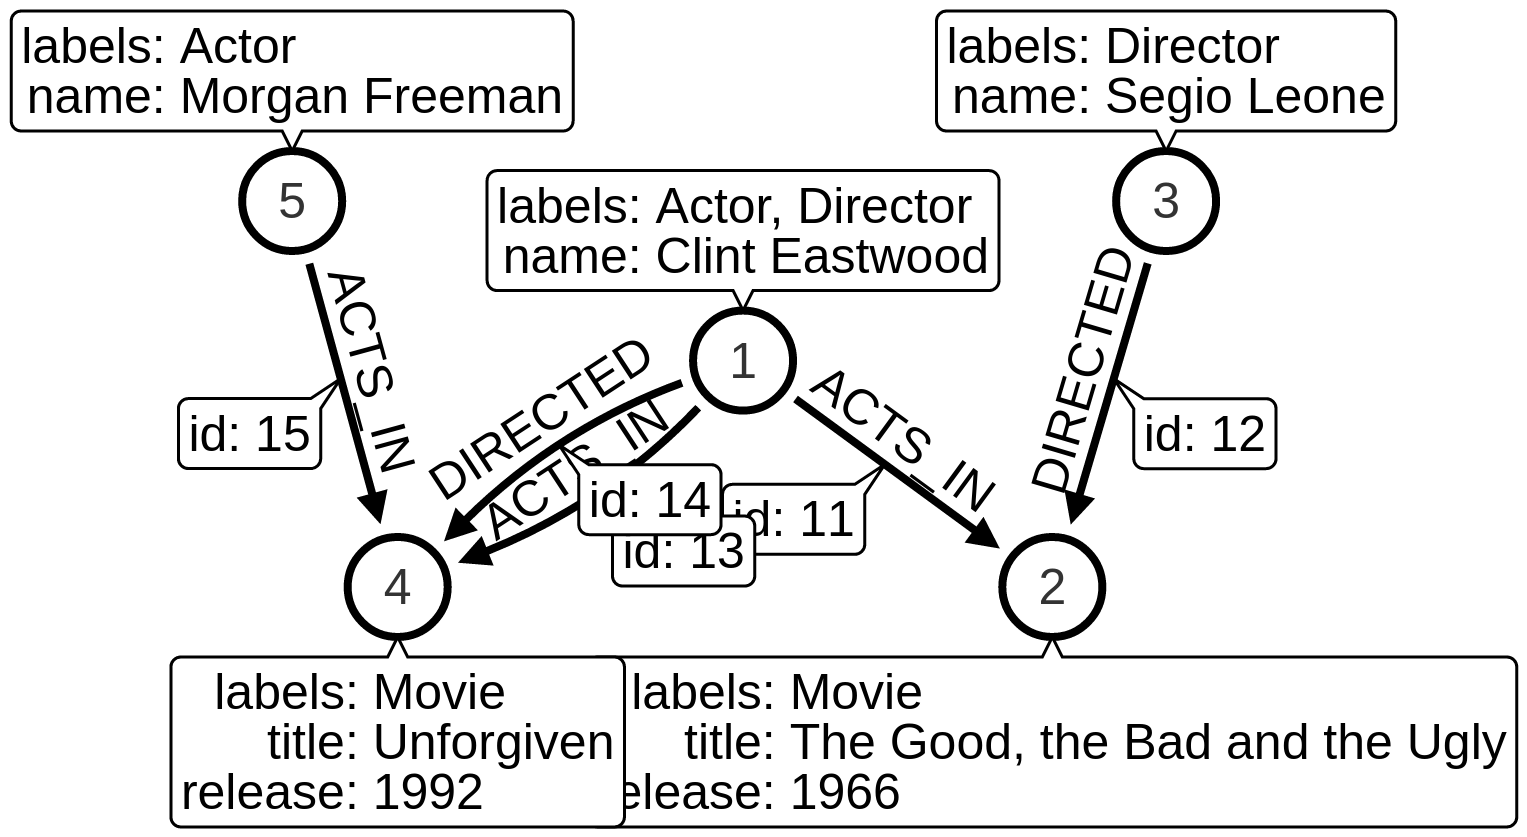
\includegraphics[width=6cm]{movie-graph}
	\captionof{figure}{Example movie graph.}
	\label{fig:running-example-property-graph}
\end{minipage}
\begin{minipage}[b]{0.53\linewidth}
	\footnotesize
	$V=\{1, 2, 3, 4, 5\}; E=\{11,12,13,14,15\};$
	
	$\verticestoedges(11) = \tuple{1, 2}; \verticestoedges(12) = \tuple{3, 2}; \ldots$

	$\vertexlabels = \{\atom{Actor}, \atom{Director}, \atom{Movie}\};$

	$\edgelabels = \{\atom{ACTS\_IN}, \atom{DIRECTED}\};$

	$\vertexlabelfunction(1) = \{\atom{Actor}, \atom{Director}\}; \vertexlabelfunction(2) = \{\atom{Movie}\}; \ldots;$

	$\edgelabelfunction(11) = \atom{ACTS\_IN}; \edgelabelfunction(12) = \atom{DIRECTED}; \ldots;$

	$\vertexproperties = \{\atom{name}, \atom{title}, \atom{release}\}; \edgeproperties = \{\};$

	$\propertyfunction{name}{1} = \atom{'Clint~Eastwood'}; \propertyfunction{name}{2} = \relnull; \ldots$

	$\propertyfunction{title}{1} = \relnull; \propertyfunction{title}{2} = \atom{'The~Good,~the~Bad~and~the~Ugly'}; \ldots$
	
	$\propertyfunction{release}{1} = \relnull; \propertyfunction{release}{2} = \atom{1966}; \ldots$
	\captionof{figure}{The dataset represented as a property graph.}
	\label{fig:property-graph-formalized}
\end{minipage}

In the context of this paper, we define a \emph{relation} as a bag (\emph{multiset}) of tuples: a tuple can occur more than once in the relation~\cite{DBLP:books/daglib/0020812}.
Given a property graph $G$, relation $r$ is a \emph{graph relation} if the following holds:
$$\forall A \in \attr{r}: \dom{A} \subseteq V \union E \union D,$$
where $\attr{r}$ is the set of attributes of $r$, $\dom{A}$ is the domain of attribute $A$. The schema of $r$, $\schema{r}$ is a list containing the attribute names. For schema transformations, the \appendtext operator is denoted by $\append$, the \removetext operator is denoted by $\remove$.

\subsection{Foundations of Relational Algebra}

\paragraph{Basic operators of relational algebra.} We give a brief summary of the operators in relational algebra. A more detailed discussion is available in database textbooks, \eg~\cite{DBLP:books/daglib/0006733}.

\paragraph{Unary operators.} The \projectiontext operator $\projectionop$ keeps a specific set of attributes in the relation: $ t = \projection{A_1, \ldots, A_n} \left(r\right).$ Note that the tuples are not deduplicated by default, \ie the results will have the same number of tuples as the input relation $r$. The projection operator can also rename the attributes, \eg $\projection{v1 \assign v2} \left(r\right)$ renames $\atom{v1}$ to $\atom{v2}$.
The \selectiontext operator $\selectionop$ filters the incoming relation according to some criteria. Formally,
$ t = \selection{\theta} \left(r\right), $
where predicate $\theta$ is a propositional formula. The operator selects all tuples in $r$ for which $\theta$ holds.

\paragraph{Binary operators.} The $\unionop$ operator produces the set union of two relations, while the $\bagunionop$ operator produces the \emph{bag union} of two operators, \eg $\{\tuple{1, 2}, \tuple{1, 2}, \tuple{3, 4}\} \bagunionop \{\tuple{1, 2}\} = \{\tuple{1, 2}, \tuple{1, 2}, \tuple{1, 2}, \tuple{3, 4}\}$. For both the \uniontext and \baguniontext operators, the schema of the operands must have the same number of attributes. Some authors also require that they share a common schema, \ie have the same set of attributes~\cite{DBLP:books/daglib/0020812}.

The $\cartesianproductop$ operator produces the \cartesianproducttext:

$$ t = r \cartesianproductop s.$$

The result of the \jointext operator $\joinop$ is determined by creating the Cartesian product of the relations, then filtering those tuples which are equal on the attributes that share a common name. The combined tuples are projected: from the attributes present in both of the two input relations, we only keep the ones in $r$ and drop the ones in $s$. Thus, the join operator is defined as
$$r \join s = \pi_{R \union S} \left(\selection{r.A_1 = s.A_1\,\land\,\ldots\,\land\,r.A_n = s.A_n)} \left(r \times s\right) \right),$$
where $ \{ A_1, \ldots, A_n \} $ is the set of attributes that occur both in $R$ and $S$, \ie $ R \intersection S = \{ A_1, \ldots, A_n \} $. Note that if the set of common attributes is empty, the \jointext operator is equivalent to the Cartesian product of the relations.
The join operator is both commutative and associative: $r \join s = s \join r$ and $(r \join s) \join t = r \join (s \join t)$, respectively.

The \antijointext operator $\antijoinop$ (also known as \emph{left anti semijoin}) collects the tuples from the left relation $r$ which have no matching pair in the right relation $s$:
$$ t = r \antijoin s = r \setminus \pi_{R} \left(r \join s\right), $$
where $\pi_{R}$ denotes a projection operator, which only keeps the attributes of the schema over relation $r$. The antijoin operator is not commutative and not associative.

The \leftouterjointext $\myleftouterjoin$ pads tuples from the left relation that did not match any from the right relation with $\relnull$ values and adds them to the result of the \jointext~\cite{DBLP:books/daglib/0015084}:
$$ t = r \myleftouterjoin s = (r \join s) \union (r \antijoin s) \cartesianproductop \{\relnull, \ldots, \relnull\}, $$

where the constant relation $\{\relnull, \ldots, \relnull\}$ is on the schema $S \setminus R$.

\subsection{Common Extensions to Relational Algebra}

Most textbooks also define \emph{extended operators} of relational algebra~\cite{DBLP:books/daglib/0020812}:

\begin{itemize}
	\item The \duplicateeliminationtext operator $\duplicateeliminationop$ eliminates duplicate tuples in a bag.
	\item The \groupingtext operator $\groupingop$ groups tuples according to their value in one or more attributes and aggregates the remaining attributes. %Aggregated values (scalars and inline collections) makes \rga not closed under \groupingtext.
	\item The \sorttext operator $\sortop$ transforms a bag relation of tuples to a list of tuples by ordering them. The ordering is defined by specified attributes of the tuples with an ordering direction (ascending $\asc$/descending $\desc$) for each attribute, \eg $\sortop_{\asc \atom{v1}, \desc \atom{v2}} (r)$.
\end{itemize}

The \toptext operator $\topp{l}{s}$ (adapted from~\cite{DBLP:conf/sigmod/LiCIS05}) takes a list as its input, skips the top $s$ tuples and returns the next $l$ tuples.\footnote{SQL implementations offer the \texttt{OFFSET} and the \texttt{LIMIT}/\texttt{TOP} keywords.}

\subsection{Graph-Specific Extensions to Relational Algebra}
\label{sec:rga}

We adapted graph-specific operators from~\cite{DBLP:conf/edbt/HolschG16}\footnote{The \textsc{GetNodes} operator introduced in~\cite{DBLP:conf/edbt/HolschG16} and did not support labels. We extended it by allowing the specification of vertex labels and renamed it to \getverticestext to be consistent with the rest of the definitions. We also extended the \textsc{ExpandIn} and \textsc{ExpandOut} operators to allow it to return a set of edges, and introduced the \expandbothtext operator to allow navigation to both directions.} and propose an additional operator.

The \getverticestext nullary operator $\getvertices{v}{t_1 \land \ldots \land t_n}$ returns a graph relation of a single attribute $v$ that contains the ID of all vertices that have \emph{all} of labels $t_1, \ldots, t_n$.

The \expandbothtext unary operator $\expandboth{E}{l_1 \lor \ldots \lor l_k \ast min \ldots max}{v}{w}{t_1 \land \ldots \land t_n}(r)$ adds (1)~a new attribute $w$ to $r$ containing the IDs of vertices having \emph{all} labels $t_1, \ldots, t_n$ that can be reached from vertices of attribute $v$ by traversing edges having \emph{any} labels $l_1, \ldots, l_n$, and (2)~a new attribute $E$ for the edges of the path from $v$ to $w$. The operator may use at least $\atom{min}$ and at most $\atom{max}$ hops, both defaulting to $1$ if omitted. % With the default setting, \ie $\atom{min}=\atom{max}=1$, a single edge variable $e$ can be used instead of edge list $E$.
The \expandintext operator~$\expandinop$ and \expandouttext operator~$\expandoutop$ only consider directed paths from $w$ to $v$ and from $v$ to $w$, respectively.

We propose the \alldifferenttext operator to guarantee the uniqueness of edges (see the remark on \emph{uniqueness of edges} in \autoref{sec:opencypher}). The \alldifferenttext operator $\alldifferent{E_1, E_2, E_3, \ldots}{(r)}$ filters $r$ to keep tuples where the variables in $\bigcup_{i} E_{i}$ are pairwise different.\footnote{Should e.g. $E_2$ be a set of the single variable $e_2$, the variable name can be used as a shorthand instead, so $\alldifferent{E_1, e_2, E_3, \ldots}{(r)} ~ \equiv ~ \alldifferent{E_1, \{e_2\}, E_3, \ldots}{(r)}$}
It can be expressed as a \selectiontext:
$$\alldifferent{E_1, E_2, E_3, \ldots}{(r)} = \selection{ \bigwedge\limits_{e_1, e_2 \,\in\, \bigcup\limits_{i} {E_i} ~ \wedge ~ { e_1 \,\neq\, e_2 } } { r.e_1 \,\neq\, r.e_2 } }{(r)}$$

\paragraph{Property access.} Assuming that $x$ is an attribute of a graph relation, we use the notation $x.a$ in (1)~attribute lists for projections and (2)~selection conditions to express the access to the corresponding value of property $a$ in the property graph~\cite{DBLP:conf/edbt/HolschG16}.

\paragraph{Summary.} \autoref{table:collections} provides an overview of the operators of \rga.

\newcommand{\propheader}{\multirow{2}{*}{\bf prop.}}
\newcommand{\rgaheader}{\multirow{2}{*}{\breakable{\bf RGA}}}

\setlength\tabcolsep{3.6pt}
\begin{table}[htb]
	\centering
	\begin{tabular}{||c||c|c|c||c|c|c||c||c||}
		\hline
		\multirow{2}{*}{\bf ops} &             \multirow{2}{*}{\bf operator}             &         \multirow{2}{*}{\bf name}         & \propheader & \multicolumn{3}{c||}{\bf output for} &             \multirow{2}{*}{\bf schema}              \\ \cline{5-7}
		&                                                       &                                           &             & \bf set & \bf bag &     \bf list     &  \\ \hline\hline
		\multirow{1}{*}{\bf 0}   &                  $\getvertices{v}{}$                  &             \getverticestext              &     set     &   set   &   set   &       set        &                  $\tuple{\atom{v}}$                  \\ \hline\hline %\cline{2-8}
%		&              $\getedges{v}{}{w}{}{e}{}$               &               \getedgestext               &     $-$     &   $-$   &   $-$   &       $-$        &               $\tuple{\atom{v, e, w}}$               \\ \hline\hline
		\multirow{8}{*}{\bf 1}   &         $\projection{v_1, v_2, \ldots} (r)$         &              \projectiontext              &      i      &   bag   &   bag   &       list       &         $\tuple{\atom{v_1, v_2, \ldots}}$          \\ \cline{2-8}
		&              $\selection{condition} (r)$              &              \selectiontext               &      i      &   set   &   bag   &       list       &                     $\schema{r}$                     \\ \cline{2-8}
		&            $\expandboth{v}{w}{}{e}{} (r)$             &              \expandbothtext              &     $-$     &   set   &   bag   &       list       &       $\schema{r} \append \tuple{\atom{e, w}}$       \\ \cline{2-8}
		&            $\alldifferent{variables} (r)$             &             \alldifferenttext             &      i      &   set   &   bag   &       list       &                     $\schema{r}$                     \\ \cline{2-8}
		&             $\duplicateeliminationop (r)$             &         \duplicateeliminationtext         &      i      &   set   &   set   &       list       &                     $\schema{r}$                     \\ \cline{2-8}
		&                     $\sort{\desc \atom{v_1}, \asc \atom{v_2}, \ldots} (r)$                     &                 \sorttext                 &      i      &  list   &  list   &       list       &                     $\schema{r}$                     \\ \cline{2-8}
		&          $\grouping{v_1, v_2, \ldots} (r)$          &               \groupingtext               &      i      &   set   &   set   &       set        &         $\tuple{\atom{v_1, v_2, \ldots}}$          \\ \cline{2-8}
		&                     $\topop (r)$                      &                 \toptext                  &     $-$     &  list   &  list   &       list       &                     $\schema{r}$                     \\ \hline\hline
		\multirow{5}{*}{\bf 2}   & $r \unionop s$, $r \minusop s$ & \uniontext, \minustext &     $-$     &   set   &   set   &       set        &                     $\schema{r}$                     \\ \cline{2-8}
		&                    $r \bagunion s$                    &               \baguniontext               &    c, a     &   bag   &   bag   &       bag        &                     $\schema{r}$                     \\ \cline{2-8}
		&               $r \cartesianproductop s$               &           \cartesianproducttext           &    c, a     &   set   &   bag   &       bag        &           $\schema{r} \append \schema{s}$            \\ \cline{2-8}
		&                    $r \joinop s$                      &                 \jointext                 &    c, a     &   set   &   bag   &       bag        & $\schema{r} \append (\schema{s} \minus \schema{r}) $ \\ \cline{2-8}
		&                $r \myleftouterjoin s$                 &            \leftouterjointext             &     $-$     &   set   &   bag   &       bag        & $\schema{r} \append (\schema{s} \minus \schema{r}) $ \\ \cline{2-8}
		&                   $r \antijoinop s$                   &               \antijointext               &    c, a     &   set   &   bag   &       bag        &                     $\schema{r}$                     \\ \cline{1-8}
	\end{tabular}
	\caption{Properties of relational graph algebra operators. A unary operator $\alpha$ is idempotent~(i), iff $\alpha(x) = \alpha(\alpha(x))$ for all inputs. A binary operator $\beta$ is commutative~(c), iff $x~\beta~y = y~\beta~x$ and associative~(a), iff $(x~\beta~y)~\beta~z = x~\beta~(y~\beta~z)$.}
	\label{table:collections}
\end{table}


\section{The openCypher Query Language}
\label{sec:opencypher}

\paragraph{Language.} As the primary query language of Neo4j~\cite{Neo4j}, Cypher~\cite{Cypher} was designed to read easily. It allows users to specify the graph pattern by a syntax resembling an actual graph. The goal of the \opencypher project~\cite{openCypher} is to provide a standardised specification of the Cypher language.
\cref{lst:example} shows an \opencypher query, which returns all people who (1)~are both actors and directors and (2)~have acted in a movie together with $\atom{Clint~Eastwood}$.

\begin{minipage}{\linewidth}
\begin{lstlisting}[label=lst:example, caption={Get people who are both actors and directors and acted in a movie with Clint Eastwood.}]
MATCH (a1)-[:ACTS_IN]->(:Movie)<-[:ACTS_IN]-(a2:Actor:Director)
WHERE a1.name = "Clint Eastwood"
RETURN a2
\end{lstlisting}
\end{minipage}

The query returns with a bag of vertices that have both the labels $\atom{Actor}$ and $\atom{Director}$ and share a common $\atom{Movie}$ neighbor through $\atom{ACTS\_IN}$ edges. Cypher guarantees that these edges are only traversed once, so the vertex of $\atom{Clint~Eastwood}$ is not returned (see the section on the uniqueness of edges).

\paragraph{Implementation.} While Neo4j uses a parsing expression grammar (PEG)~\cite{DBLP:conf/popl/Ford04} for specifying the grammar rules of Cypher, openCypher aims to achieve an implementation-agnostic specification by only providing a context-free grammar. The parser can be implemented using any capable parser technology, \eg \antlr~\cite{Parr:2013:DAR:2501720} or Xtext~\cite{DBLP:conf/oopsla/EysholdtB10}. %It also possible to generate a grammar following the ISO 14977 Extended Backus--Naur Form~\cite{ISO14977},

\paragraph{Legacy grammar rules.} It is not a goal of the openCypher project to fully cover the features of Neo4j's Cypher language: ``Not all grammar rules of the Cypher language will be standardised in their current form, meaning that they will not be part of openCypher as-is. Therefore, the openCypher grammar will not include some well-known Cypher constructs; these are called 'legacy'.''\footnote{\url{https://github.com/opencypher/openCypher/tree/master/grammar}} The \emph{legacy rules} include commands (\lstinline+CREATE INDEX+, \lstinline+CREATE UNIQUE CONSTRAINT+, etc.), pre-parser rules (\lstinline+EXPLAIN+, \lstinline+PROFILE+) and deprecated constructs (\lstinline+START+). A detailed description is provided in the openCypher specification. In our work, we focused on the \emph{standard core} of the language and ignored legacy rules.

% http://neo4j.com/docs/developer-manual/current/cypher/#cypherdoc-uniqueness
\paragraph{Uniqueness for edges.} In an \opencypher query, a \lstinline+MATCH+ clause defines a graph pattern. A query can be composed of multiple patterns spanning multiple \lstinline+MATCH+ clauses. For the matches of a pattern within a single \lstinline+MATCH+ clause, edges are required to be unique. %even for disconnected graph patterns.
However, matches for multiple \lstinline+MATCH+ clauses can share edges. This uniqueness criterium can be expressed in a compact way with the \alldifferenttext operator introduced in \cref{sec:rga}. For vertices, this restriction does not apply.

\paragraph{Aggregation.} It indeed makes sense to calculate aggregation over graph pattern matches, though, its result will not necessarily be pattern match with vertices and edges. Based on some \emph{grouping criteria}, matches are put into categories, and values for the grouping criteria as well as grouping functions\footnote{For example, \lstinline+count+, \lstinline+avg+, \lstinline+sum+, \lstinline+max+, \lstinline+min+, \lstinline+stdDev+, \lstinline+stdDevP+, \lstinline+collect+. The \lstinline+collect+ function is an exception as it does not return a single scalar value but returns a collection (list).} over the groups, the aggregations are evaluated in a single tuple for each and every category. In the SQL query language, grouping criteria is explicitly given by using the \lstinline+GROUP BY+ clause. In \opencypher, however, this is done implicitly in the \lstinline+RETURN+ as well as in \lstinline+WITH+ clauses: vertices, edges and their properties that appear outside the grouping functions become the \emph{grouping criteria}.\footnote{This approach is also used by some SQL code assistant IDEs generating the \lstinline+GROUP BY+ clause for a query.}

\paragraph{Subqueries.} One can compose an \opencypher query of multiple subqueries. Subqueries, written subsequently, mostly begin by a \lstinline+MATCH+ clause and end at (including) a \lstinline+RETURN+ or \lstinline+WITH+ clause, the latter having an optional \lstinline+WHERE+ clause to follow. The \lstinline+WITH+ and \lstinline+RETURN+ clauses determine the resulting schema of the subquery by specifiying the vertices, edges, attributes and aggregates of the result. When \lstinline+WITH+ has the optional \lstinline+WHERE+ clause, it applies an other filter on the subquery result.~\footnote{This is much like the \lstinline+HAVING+ construct of the SQL language with the major difference that it is also allowed in \opencypher in case no aggregation has been done.} The last subquery must be ended by \lstinline+RETURN+, whereas all the previous ones must be ended by \lstinline+WITH+. If a query is composed by more than one subqueries, their results are joined together using \jointext or \leftouterjointext operators.


\section{Mapping \opencypher Queries to \RGA}
\label{sec:compilation}

In this section, we first give the mapping algorithm of \opencypher queries to \rga, then we give a more detailed listing of the compilation rules for the query language constructs in \autoref{table:mapping}.
We follow the bottom-up approach to build the \rga tree based on the \opencypher query. The algorithm is as follows. Join operations always use all common variables to match the two inputs (see \jointext in \autoref{sec:rga}).

\setlength\tabcolsep{3.6pt}
\begin{enumerate}
\label{alg:build-rga-tree}
	\item A single pattern is turned left-to-right to a \getverticestext for the first vertex and a chain of \expandintext, \expandouttext or \expandbothtext operators for inbound, outbound or undirected relationships, respectively.
	\item Patterns in the same \lstinline+MATCH+ clause are joined by \jointext.
	\item Append an \alldifferenttext operator for all edge variables that appear in the \lstinline+MATCH+ clause because of the non-repeating edges language rule.
	\item Process the \lstinline+WHERE+ clause. Note that according to the grammar, \lstinline+WHERE+ is bound to a \lstinline+MATCH+ clause.
	\item Several \lstinline+MATCH+ clauses are connected to a left deep tree of \jointext. If \lstinline+MATCH+ has the \lstinline+OPTIONAL+ modifier, \leftouterjointext is used instead of \jointext.
	\item If there is a positive or negative pattern deferred from \lstinline+WHERE+ processing,
		append it as a \jointext or \antijointext operator, respectively.
	\item Append \groupingtext, if \lstinline+RETURN+ or \lstinline+WITH+ clause has grouping functions inside
	\item Append \projectiontext operator based on the \lstinline+RETURN+ or \lstinline+WITH+ clause. This operator will also handle the renaming (i.e. \lstinline+AS+).
	\item Append \duplicateeliminationtext operator, if the \lstinline+RETURN+ or \lstinline+WITH+ clause has the \lstinline+DISTINCT+ modifier.
	\item Append a \selectiontext operator in case the \lstinline+WITH+ had the optional \lstinline+WHERE+ clause.
	\item If this is not the first subquery, join to the \rga tree using \jointext or \leftouterjointext.
	\item Assemble a \uniontext operation from the query parts\footnote{In this context, query parts refer to those parts of the query connected by the \lstinline+UNION+ \opencypher keyword.}. As the \uniontext operator is technically a binary operator, the \uniontext of more than two query parts are represented as a left deep tree of \lstinline+UNION+ operators.
\end{enumerate}

\setlength\extrarowheight{2.5pt}
\setlength\tabcolsep{3.6pt}
\begin{table}[htbp]
	\centering
	\begin{tabular}{|l|l|l|}
		\hline
		\multicolumn{2}{|l|}{ \bf Language construct } & \bf Relational algebra expression \\ \hline\hline

		%\hline
		\multicolumn{3}{|l|}{Vertex, edge and path patterns } \\ \cline{2-3}

		& \lstinline+()+ & $\getvertices{\_v}{}$ \\ \cline{2-3}

		& \lstinline+(:types)+ & $\getvertices{\_v}{types}$ \\ \cline{2-3}

		& \lstinline+(<v>v</v>:types)+ & $\getvertices{v}{types}$ \\ \cline{2-3}

		% expand operators
		& \lstinline+<v>p</v>-[<v>e</v>:<v>labels</v>]-(<v>w</v>:types...)+ & \multirow{2}{*}{$\expandboth{v}{w}{types}{e}{labels}{1}{1} (\atom{p})$} \\ \cline{2-2}

		& \lstinline+<v>p</v><-[<v>e</v>:<v>labels</v>]->(<v>w</v>:types...)+ & \\ \cline{2-3}

		& \lstinline+<v>p</v>-[<v>e</v>:<v>labels</v>]->(<v>w</v>:types...)+ & $\expandout{v}{w}{types}{e}{labels}{1}{1} (\atom{p})$ \\ \cline{2-3}

		& \lstinline+<v>p</v><-[<v>e</v>:<v>labels</v>]-(<v>w</v>:types...)+ & $\expandin{v}{w}{types}{e}{labels}{1}{1} (\atom{p})$ \\ \cline{2-3}

		& \lstinline+<v>p</v>-[<v>E</v>:<v>labels</v>*<v>min</v>..<v>max</v>]->(<v>w</v>:<v>t2</v>)+ & $\expandout{v}{w}{types}{E}{labels}{min}{max}(\atom{p})$ \\ \cline{2-3}

		& \lstinline+<v>p</v>-[<v>E</v>:<v>labels</v>*]->(<v>w</v>:<v>t2</v>)+ & $\transitiveclosureout{v}{w}{types}{E}{labels}(\atom{p})$ \\ \cline{2-3}

		\hline \multicolumn{3}{|l|}{Combining and filtering pattern matches } \\ \cline{2-3}

		& \lstinline+MATCH <v>p</v>+ & $\alldifferent{\atom{edges~of~p}} \left(\atom{p}\right)$ \\ \cline{2-3}

		& \lstinline+MATCH <v>p1</v>, <v>p2</v>+ &
		$\alldifferent{\atom{edges~of~p1~and~p2}} \left( \atom{p_1}~\join~\atom{p_2} \right)$ \\ \cline{2-3}

		& \breakable{
			\lstinline+MATCH <v>p1</v>+ \\
			\lstinline+MATCH <v>p2</v>+
		} &
		$\alldifferent{\atom{edges~of~p1}} \left(\atom{p_1}\right)~\join~\alldifferent{\atom{edges~of~p2}} \left(\atom{p_2}\right)$ \\ \cline{2-3}

		& \breakable{
			\lstinline+MATCH <v>p1</v>+ \\
			\lstinline+OPTIONAL MATCH <v>p2</v>+
		} & $\alldifferent{\atom{edges~of~p1}} \left(\atom{p_1}\right)~\myleftouterjoin~\alldifferent{\atom{edges~of~p2}} \left(\atom{p_2}\right)$ \\ \cline{2-3}

		& \breakable{
			\lstinline+MATCH <v>p</v>+ \\
			\lstinline+WHERE <v>condition</v>+
		} & \breakable{$\selection{\atom{condition}}{\left( r \right)}$, where $\atom{condition}$ may \tabularnewline specify patterns and arithmetic \tabularnewline constraints on existing variables} \\ \cline{2-3}

		\hline \multicolumn{3}{|l|}{Result and sub-result operations. Rules for \lstinline+RETURN+ also apply to \lstinline+WITH+.} \\ \cline{2-3}

		& \lstinline+RETURN <v>variables</v>+ & $\projection{\atom{variables}}{\left( r \right)}$ \\ \cline{2-3}

		& \lstinline+RETURN <v>v1</v> AS <v>alias1</v> ...+ & $\projection{\atom{v1} \assign \atom{alias1}, \ldots }\left( r \right)$ \\ \cline{2-3}

		& \lstinline+RETURN DISTINCT <v>variables</v>+ & $\duplicateelimination\left(\projection{\atom{variables}}{\left( r \right)}\right)$ \\ \cline{2-3}

		& \lstinline+RETURN <v>variables</v>, <v>aggregates</v>+ & $\grouping{\atom{variables}, \atom{aggregates}}{\left( r \right)}$ \\ \cline{2-3}

		\hline \multicolumn{3}{|l|}{List operations } \\ \cline{2-3}

		& \lstinline+ORDER BY <v>v1</v> [ASC|DESC] ...+ & $\sort{\asc/\desc \atom{v1}, \ldots}{\left( r \right)}$ \\ \cline{2-3}

		& \lstinline+LIMIT <v>l</v>+ & $\limit{l}(r)$ \\ \cline{2-3}

		& \lstinline+SKIP <v>s</v>+ & $\skipp{s}(r)$ \\ \cline{2-3}

		& \lstinline+SKIP <v>s</v> LIMIT <v>l</v>+ & $\topp{l}{s}(r)$ \\ \cline{2-3}

		\hline \multicolumn{3}{|l|}{Combining results } \\ \cline{2-3}

		& \lstinline+<v>query1</v> UNION <v>query2</v>+ & $r_1 \union r_2$ \\ \cline{2-3}

		& \lstinline+<v>query1</v> UNION ALL <v>query2</v>+ & $r_1 \bagunion r_2$ \\ \hline
	\end{tabular}
	\caption{Mapping from \opencypher constructs to relational algebra.}
	\label{table:mapping}
\end{table}

\paragraph{Example.} The example query in~\autoref{lst:example} can be formalized as:
{\footnotesize
	\begin{align*}
	&\projection{a2} \Bigg(\selection{a1.name = 'C.\,E.'} \Big( \alldifferent{\_e1, \_e2} \expandin{a1}{a2}{Actor \land Director}{\_e1}{ACTS\_IN}{1}{1} \expandout{a1}{}{Movie}{\_e2}{ACTS\_IN}{1}{1} \left(\getvertices{a1}{Actor}\right) \Big) \Bigg)
	\end{align*}
}

Note that the $\alldifferentop$ guarantees the uniqueness constraint for the edges (\autoref{sec:opencypher}), which prevents the query from returning the vertex $\atom{Clint~Eastwood}$.

\paragraph{Optimisations.} Queries with negative conditions for patterns can also be expressed using the \antijointext operator. For example, \lstinline+MATCH <v>p1</v> WHERE NOT <v>p2</v>+ can be formalized as
$$\alldifferent{\atom{edges~of~p1}} \left(\atom{p_1}\right) \antijoin \alldifferent{\atom{edges~of~p2}} \left(\atom{p_2}\right)$$

\paragraph{Limitations.} Our mapping does not completely cover the \opencypher language. As discussed in \autoref{sec:opencypher}, some constructs are defined as legacy and thus were omitted. Also, we did not formalize expressions (\eg  conditions in selections), collections (arrays and maps), which are required for both path variables\footnote{\lstinline+MATCH p=(:Person)-[:FRIEND*1..2]->(:Person)+} and the \lstinline+UNWIND+ operator. The mapping does not cover parameters and data manipulation operations, \eg \lstinline+CREATE+, \lstinline+DELETE+, \lstinline+SET+ and \lstinline+MERGE+.


\section{Related Work}
\label{sec:related-work}

The TinkerPop framework~\cite{TinkerPop} aims to provide a standard data model for property graphs, along with Gremlin, a high-level graph-traversal language~\cite{Rodriguez:2015:GGT:2815072.2815073} and the Gremlin Structure API, a low-level programming interface.

Besides property graphs, graph queries can be formalized on different graph-like data models and even relational databases.

\paragraph{EMF.} The Eclipse Modeling Framework (EMF) is an object-oriented modelling framework widely used in model-driven engineering. 
Henshin~\cite{DBLP:conf/models/ArendtBJKT10} provides a visual language for defining patterns, while Epsilon~\cite{DBLP:conf/icmt/KolovosPP08} and \viatraquery~\cite{DBLP:conf/models/BergmannHRVBBO10} provide high-level declarative (textual) query languages, Epsilon Pattern Language and \vql.

\paragraph{RDF.} The Resource Description Framework (RDF)~\cite{RDF} aims to describe entities of the semantic web. RDF assumes sparse, ever-growing and incomplete data stored as triples that can be queried using the \sparql~\cite{SPARQL} graph pattern language.
%A formal definition of the \sparql language is given in~\cite{DBLP:journals/tods/PerezAG09}.

\lstset{language=}

\paragraph{SQL.} In general, relational databases offer limited support for graph queries: recursive queries are supported by \mbox{PostgreSQL} using the \lstinline+WITH RECURSIVE+ keyword and by the Oracle Database using the \lstinline+CONNECT BY+ keyword. Graph queries are supported in \saphana Graph
Scale-Out Extension prototype~\cite{DBLP:conf/btw/RudolfPBL13}, through a SQL-based language~\cite{DBLP:conf/gg/KrauseJDSKN16}.


\section{Conclusion and Future Work}
\label{sec:conclusion}

In this paper, we presented a formal specification for a subset of the \opencypher query language. This provides the theoretical foundations to use \opencypher as a language for graph query engines. Using the proposed mapping, an \opencypher-compliant query engine could be built on any relational database engine to (1)~store property graphs as graph relations and to (2)~efficiently evaluate the extended operators of \rga.

As a future work, we will give formal specification of the operators for incremental query evaluation, which requires us to define \emph{maintenance operations} to keep their result in sync with the latest set of changes. Our long-term research objective is to design and prototype a \emph{distributed, incremental graph query engine}~\cite{DBLP:conf/models/SzarnyasIRHBV14} for the property graph data model.



\chapter{TCK Acceptance Tests}

\section{AggregationAcceptance}

\subsection{Support multiple divisions in aggregate function}

\subsubsection*{Query specification}

\begin{lstlisting}
MATCH (n)
RETURN count(n) / 60 / 60 AS count
\end{lstlisting}

\subsubsection*{Relational algebra expression}

Cannot convert to expression.

\subsubsection*{Relational algebra tree}

Cannot visualize tree.

\subsubsection*{Relational algebra tree for incremental queries}

Cannot visualize incremental tree.

\subsection{Support column renaming for aggregates as well}

\subsubsection*{Query specification}

\begin{lstlisting}
MATCH ()
RETURN count(*) AS columnName
\end{lstlisting}

\subsubsection*{Relational algebra expression}

Cannot convert to expression.

\subsubsection*{Relational algebra tree}

Cannot visualize tree.

\subsubsection*{Relational algebra tree for incremental queries}

Cannot visualize incremental tree.

\subsection{Aggregates inside normal functions}

\subsubsection*{Query specification}

\begin{lstlisting}
MATCH (a)
RETURN size(collect(a))
\end{lstlisting}

\subsubsection*{Relational algebra expression}

Cannot convert to expression.

\subsubsection*{Relational algebra tree}

Cannot visualize tree.

\subsubsection*{Relational algebra tree for incremental queries}

Cannot visualize incremental tree.

\subsection{Handle aggregates inside non-aggregate expressions}

\subsubsection*{Query specification}

\begin{lstlisting}
MATCH (a {name: 'Andres'})<-[:FATHER]-(child)
RETURN {foo: a.name='Andres', kids: collect(child.name)}
\end{lstlisting}

\subsubsection*{Relational algebra expression}

Cannot convert to expression.

\subsubsection*{Relational algebra tree}

Cannot visualize tree.

\subsubsection*{Relational algebra tree for incremental queries}

Cannot visualize incremental tree.

\subsection{Count nodes}

\subsubsection*{Query specification}

\begin{lstlisting}
MATCH (a:L)-[rel]->(b)
RETURN a, count(*)
\end{lstlisting}

\subsubsection*{Relational algebra expression}

Cannot convert to expression.

\subsubsection*{Relational algebra tree}

Cannot visualize tree.

\subsubsection*{Relational algebra tree for incremental queries}

Cannot visualize incremental tree.

\subsection{Sort on aggregate function and normal property}

\subsubsection*{Query specification}

\begin{lstlisting}
MATCH (n)
RETURN n.division, count(*)
ORDER BY count(*) DESC, n.division ASC
\end{lstlisting}

\subsubsection*{Relational algebra expression}

Cannot convert to expression.

\subsubsection*{Relational algebra tree}

Cannot visualize tree.

\subsubsection*{Relational algebra tree for incremental queries}

Cannot visualize incremental tree.

\subsection{Aggregate on property}

\subsubsection*{Query specification}

\begin{lstlisting}
MATCH (n)
RETURN n.x, count(*)
\end{lstlisting}

\subsubsection*{Relational algebra expression}

Cannot convert to expression.

\subsubsection*{Relational algebra tree}

Cannot visualize tree.

\subsubsection*{Relational algebra tree for incremental queries}

Cannot visualize incremental tree.

\subsection{Count non-null values}

\subsubsection*{Query specification}

\begin{lstlisting}
MATCH (n)
RETURN n.y, count(n.x)
\end{lstlisting}

\subsubsection*{Relational algebra expression}

Cannot convert to expression.

\subsubsection*{Relational algebra tree}

Cannot visualize tree.

\subsubsection*{Relational algebra tree for incremental queries}

Cannot visualize incremental tree.

\subsection{Sum non-null values}

\subsubsection*{Query specification}

\begin{lstlisting}
MATCH (n)
RETURN n.y, sum(n.x)
\end{lstlisting}

\subsubsection*{Relational algebra expression}

Cannot convert to expression.

\subsubsection*{Relational algebra tree}

Cannot visualize tree.

\subsubsection*{Relational algebra tree for incremental queries}

Cannot visualize incremental tree.

\subsection{Handle aggregation on functions}

\subsubsection*{Query specification}

\begin{lstlisting}
MATCH p=(a:L)-[*]->(b)
RETURN b, avg(length(p))
\end{lstlisting}

\subsubsection*{Relational algebra expression}

Cannot convert to expression.

\subsubsection*{Relational algebra tree}

Cannot visualize tree.

\subsubsection*{Relational algebra tree for incremental queries}

Cannot visualize incremental tree.

\subsection{Distinct on unbound node}

\subsubsection*{Query specification}

\begin{lstlisting}
OPTIONAL MATCH (a)
RETURN count(DISTINCT a)
\end{lstlisting}

\subsubsection*{Relational algebra expression}

Cannot convert to expression.

\subsubsection*{Relational algebra tree}

Cannot visualize tree.

\subsubsection*{Relational algebra tree for incremental queries}

Cannot visualize incremental tree.

\subsection{Distinct on null}

\subsubsection*{Query specification}

\begin{lstlisting}
MATCH (a)
RETURN count(DISTINCT a.foo)
\end{lstlisting}

\subsubsection*{Relational algebra expression}

Cannot convert to expression.

\subsubsection*{Relational algebra tree}

Cannot visualize tree.

\subsubsection*{Relational algebra tree for incremental queries}

Cannot visualize incremental tree.

\subsection{Collect distinct nulls}

\subsubsection*{Query specification}

\begin{lstlisting}
UNWIND [null, null] AS x
RETURN collect(DISTINCT x) AS c
\end{lstlisting}

\subsubsection*{Relational algebra expression}

Cannot convert to expression.

\subsubsection*{Relational algebra tree}

Cannot visualize tree.

\subsubsection*{Relational algebra tree for incremental queries}

Cannot visualize incremental tree.

\subsection{Collect distinct values mixed with nulls}

\subsubsection*{Query specification}

\begin{lstlisting}
UNWIND [null, 1, null] AS x
RETURN collect(DISTINCT x) AS c
\end{lstlisting}

\subsubsection*{Relational algebra expression}

Cannot convert to expression.

\subsubsection*{Relational algebra tree}

Cannot visualize tree.

\subsubsection*{Relational algebra tree for incremental queries}

Cannot visualize incremental tree.

\subsection{Aggregate on list values}

\subsubsection*{Query specification}

\begin{lstlisting}
MATCH (a)
RETURN DISTINCT a.color, count(*)
\end{lstlisting}

\subsubsection*{Relational algebra expression}

Cannot convert to expression.

\subsubsection*{Relational algebra tree}

Cannot visualize tree.

\subsubsection*{Relational algebra tree for incremental queries}

Cannot visualize incremental tree.

\subsection{Aggregates in aggregates}

\subsubsection*{Query specification}

\begin{lstlisting}
RETURN count(count(*))
\end{lstlisting}

\subsubsection*{Relational algebra expression}

Cannot convert to expression.

\subsubsection*{Relational algebra tree}

Cannot visualize tree.

\subsubsection*{Relational algebra tree for incremental queries}

Cannot visualize incremental tree.

\subsection{Aggregates with arithmetics}

\subsubsection*{Query specification}

\begin{lstlisting}
MATCH ()
RETURN count(*) * 10 AS c
\end{lstlisting}

\subsubsection*{Relational algebra expression}

Cannot convert to expression.

\subsubsection*{Relational algebra tree}

Cannot visualize tree.

\subsubsection*{Relational algebra tree for incremental queries}

Cannot visualize incremental tree.

\subsection{Aggregates ordered by arithmetics}

\subsubsection*{Query specification}

\begin{lstlisting}
MATCH (a:A), (b:X)
RETURN count(a) * 10 + count(b) * 5 AS x
ORDER BY x
\end{lstlisting}

\subsubsection*{Relational algebra expression}

Cannot convert to expression.

\subsubsection*{Relational algebra tree}

Cannot visualize tree.

\subsubsection*{Relational algebra tree for incremental queries}

Cannot visualize incremental tree.

\subsection{Multiple aggregates on same variable}

\subsubsection*{Query specification}

\begin{lstlisting}
MATCH (n)
RETURN count(n), collect(n)
\end{lstlisting}

\subsubsection*{Relational algebra expression}

Cannot convert to expression.

\subsubsection*{Relational algebra tree}

Cannot visualize tree.

\subsubsection*{Relational algebra tree for incremental queries}

Cannot visualize incremental tree.

\subsection{Simple counting of nodes}

\subsubsection*{Query specification}

\begin{lstlisting}
MATCH ()
RETURN count(*)
\end{lstlisting}

\subsubsection*{Relational algebra expression}

Cannot convert to expression.

\subsubsection*{Relational algebra tree}

Cannot visualize tree.

\subsubsection*{Relational algebra tree for incremental queries}

Cannot visualize incremental tree.

\subsection{Aggregation of named paths}

\subsubsection*{Query specification}

\begin{lstlisting}
MATCH p = (a)-[*]->(b)
RETURN collect(nodes(p)) AS paths, length(p) AS l
ORDER BY l
\end{lstlisting}

\subsubsection*{Relational algebra expression}

Cannot convert to expression.

\subsubsection*{Relational algebra tree}

Cannot visualize tree.

\subsubsection*{Relational algebra tree for incremental queries}

Cannot visualize incremental tree.

\subsection{Aggregation with `min()`}

\subsubsection*{Query specification}

\begin{lstlisting}
MATCH p = (a:T {name: 'a'})-[:R*]->(other:T)
WHERE other <> a
WITH a, other, min(length(p)) AS len
RETURN a.name AS name, collect(other.name) AS others, len
\end{lstlisting}

\subsubsection*{Relational algebra expression}

Cannot convert to expression.

\subsubsection*{Relational algebra tree}

Cannot visualize tree.

\subsubsection*{Relational algebra tree for incremental queries}

Cannot visualize incremental tree.

\subsection{Handle subexpression in aggregation also occurring as standalone expression with nested aggregation in a literal map}

\subsubsection*{Query specification}

\begin{lstlisting}
MATCH (a:A), (b:B)
RETURN coalesce(a.prop, b.prop) AS foo,
  b.prop AS bar,
  {y: count(b)} AS baz
\end{lstlisting}

\subsubsection*{Relational algebra expression}

Cannot convert to expression.

\subsubsection*{Relational algebra tree}

Cannot visualize tree.

\subsubsection*{Relational algebra tree for incremental queries}

Cannot visualize incremental tree.

\subsection{Projection during aggregation in WITH before MERGE and after WITH with predicate}

\subsubsection*{Query specification}

\begin{lstlisting}
UNWIND [42] AS props
WITH props WHERE props > 32
WITH DISTINCT props AS p
MERGE (a:A {prop: p})
RETURN a.prop AS prop
\end{lstlisting}

\subsubsection*{Relational algebra expression}

Cannot convert to expression.

\subsubsection*{Relational algebra tree}

Cannot visualize tree.

\subsubsection*{Relational algebra tree for incremental queries}

Cannot visualize incremental tree.

\subsection{No overflow during summation}

\subsubsection*{Query specification}

\begin{lstlisting}
UNWIND range(1000000, 2000000) AS i
WITH i
LIMIT 3000
RETURN sum(i)
\end{lstlisting}

\subsubsection*{Relational algebra expression}

Cannot convert to expression.

\subsubsection*{Relational algebra tree}

Cannot visualize tree.

\subsubsection*{Relational algebra tree for incremental queries}

Cannot visualize incremental tree.

\subsection{Counting with loops}

\subsubsection*{Query specification}

\begin{lstlisting}
MATCH ()-[r]-()
RETURN count(r)
\end{lstlisting}

\subsubsection*{Relational algebra expression}

Cannot convert to expression.

\subsubsection*{Relational algebra tree}

Cannot visualize tree.

\subsubsection*{Relational algebra tree for incremental queries}

Cannot visualize incremental tree.

\subsection{`max()` should aggregate strings}

\subsubsection*{Query specification}

\begin{lstlisting}
UNWIND ['a', 'b', 'B', null, 'abc', 'abc1'] AS i
RETURN max(i)
\end{lstlisting}

\subsubsection*{Relational algebra expression}

Cannot convert to expression.

\subsubsection*{Relational algebra tree}

Cannot visualize tree.

\subsubsection*{Relational algebra tree for incremental queries}

Cannot visualize incremental tree.

\subsection{`min()` should aggregate strings}

\subsubsection*{Query specification}

\begin{lstlisting}
UNWIND ['a', 'b', 'B', null, 'abc', 'abc1'] AS i
RETURN min(i)
\end{lstlisting}

\subsubsection*{Relational algebra expression}

Cannot convert to expression.

\subsubsection*{Relational algebra tree}

Cannot visualize tree.

\subsubsection*{Relational algebra tree for incremental queries}

Cannot visualize incremental tree.

\section{ColumnNameAcceptance}

\subsection{Keeping used expression 1}

\subsubsection*{Query specification}

\begin{lstlisting}
MATCH (n)
RETURN cOuNt( * )
\end{lstlisting}

\subsubsection*{Relational algebra expression}

Cannot convert to expression.

\subsubsection*{Relational algebra tree}

Cannot visualize tree.

\subsubsection*{Relational algebra tree for incremental queries}

Cannot visualize incremental tree.

\subsection{Keeping used expression 2}

\subsubsection*{Query specification}

\begin{lstlisting}
MATCH p = (n)-->(b)
RETURN nOdEs( p )
\end{lstlisting}

\subsubsection*{Relational algebra expression}

Cannot convert to expression.

\subsubsection*{Relational algebra tree}

Cannot visualize tree.

\subsubsection*{Relational algebra tree for incremental queries}

Cannot visualize incremental tree.

\subsection{Keeping used expression 3}

\subsubsection*{Query specification}

\begin{lstlisting}
MATCH p = (n)-->(b)
RETURN coUnt( dIstInct p )
\end{lstlisting}

\subsubsection*{Relational algebra expression}

Cannot convert to expression.

\subsubsection*{Relational algebra tree}

Cannot visualize tree.

\subsubsection*{Relational algebra tree for incremental queries}

Cannot visualize incremental tree.

\subsection{Keeping used expression 4}

\subsubsection*{Query specification}

\begin{lstlisting}
MATCH p = (n)-->(b)
RETURN aVg(    n.aGe     )
\end{lstlisting}

\subsubsection*{Relational algebra expression}

Cannot convert to expression.

\subsubsection*{Relational algebra tree}

Cannot visualize tree.

\subsubsection*{Relational algebra tree for incremental queries}

Cannot visualize incremental tree.

\section{ComparisonOperatorAcceptance}

\subsection{Handling numerical ranges 1}

\subsubsection*{Query specification}

\begin{lstlisting}
MATCH (n)
WHERE 1 < n.value < 3
RETURN n.value
\end{lstlisting}

\subsubsection*{Relational algebra expression}

$\projection{\var{n}} \left(\selection{\mathtt{1~<~n.value~<~3}} \left(\alldifferent{} \left(\getvertices{n}{}\right)\right)\right)$

\subsubsection*{Relational algebra tree}

\begin{tikzpicture}
\linespread{1.25}
\Tree
[. {$\projection{\var{n}}$ \\ \footnotesize $\color{gray} \langle \var{n} \rangle$}
	[. {$\selection{\mathtt{1~<~n.value~<~3}}$ \\ \footnotesize $\color{gray} \langle \var{n} \rangle$}
		[. {$\getvertices{n}{}$ \\ \footnotesize $\color{gray} \langle \var{n} \rangle$}
		]
	]
]
;
\end{tikzpicture}

\subsubsection*{Relational algebra tree for incremental queries}

\begin{tikzpicture}
\linespread{1.25}
\Tree
[. {$\projection{\var{n}}$ \\ \footnotesize $\color{gray} \langle \var{n} \rangle$}
	[. {$\selection{\mathtt{1~<~n.value~<~3}}$ \\ \footnotesize $\color{gray} \langle \var{n} \rangle$}
		[. {$\getvertices{n}{}$ \\ \footnotesize $\color{gray} \langle \var{n} \rangle$}
		]
	]
]
;
\end{tikzpicture}

\subsection{Handling numerical ranges 2}

\subsubsection*{Query specification}

\begin{lstlisting}
MATCH (n)
WHERE 1 < n.value <= 3
RETURN n.value
\end{lstlisting}

\subsubsection*{Relational algebra expression}

$\projection{\var{n}} \left(\selection{\mathtt{1~<~n.value~<=~3}} \left(\alldifferent{} \left(\getvertices{n}{}\right)\right)\right)$

\subsubsection*{Relational algebra tree}

\begin{tikzpicture}
\linespread{1.25}
\Tree
[. {$\projection{\var{n}}$ \\ \footnotesize $\color{gray} \langle \var{n} \rangle$}
	[. {$\selection{\mathtt{1~<~n.value~<=~3}}$ \\ \footnotesize $\color{gray} \langle \var{n} \rangle$}
		[. {$\getvertices{n}{}$ \\ \footnotesize $\color{gray} \langle \var{n} \rangle$}
		]
	]
]
;
\end{tikzpicture}

\subsubsection*{Relational algebra tree for incremental queries}

\begin{tikzpicture}
\linespread{1.25}
\Tree
[. {$\projection{\var{n}}$ \\ \footnotesize $\color{gray} \langle \var{n} \rangle$}
	[. {$\selection{\mathtt{1~<~n.value~<=~3}}$ \\ \footnotesize $\color{gray} \langle \var{n} \rangle$}
		[. {$\getvertices{n}{}$ \\ \footnotesize $\color{gray} \langle \var{n} \rangle$}
		]
	]
]
;
\end{tikzpicture}

\subsection{Handling numerical ranges 3}

\subsubsection*{Query specification}

\begin{lstlisting}
MATCH (n)
WHERE 1 <= n.value < 3
RETURN n.value
\end{lstlisting}

\subsubsection*{Relational algebra expression}

$\projection{\var{n}} \left(\selection{\mathtt{1~<=~n.value~<~3}} \left(\alldifferent{} \left(\getvertices{n}{}\right)\right)\right)$

\subsubsection*{Relational algebra tree}

\begin{tikzpicture}
\linespread{1.25}
\Tree
[. {$\projection{\var{n}}$ \\ \footnotesize $\color{gray} \langle \var{n} \rangle$}
	[. {$\selection{\mathtt{1~<=~n.value~<~3}}$ \\ \footnotesize $\color{gray} \langle \var{n} \rangle$}
		[. {$\getvertices{n}{}$ \\ \footnotesize $\color{gray} \langle \var{n} \rangle$}
		]
	]
]
;
\end{tikzpicture}

\subsubsection*{Relational algebra tree for incremental queries}

\begin{tikzpicture}
\linespread{1.25}
\Tree
[. {$\projection{\var{n}}$ \\ \footnotesize $\color{gray} \langle \var{n} \rangle$}
	[. {$\selection{\mathtt{1~<=~n.value~<~3}}$ \\ \footnotesize $\color{gray} \langle \var{n} \rangle$}
		[. {$\getvertices{n}{}$ \\ \footnotesize $\color{gray} \langle \var{n} \rangle$}
		]
	]
]
;
\end{tikzpicture}

\subsection{Handling numerical ranges 4}

\subsubsection*{Query specification}

\begin{lstlisting}
MATCH (n)
WHERE 1 <= n.value <= 3
RETURN n.value
\end{lstlisting}

\subsubsection*{Relational algebra expression}

$\projection{\var{n}} \left(\selection{\mathtt{1~<=~n.value~<=~3}} \left(\alldifferent{} \left(\getvertices{n}{}\right)\right)\right)$

\subsubsection*{Relational algebra tree}

\begin{tikzpicture}
\linespread{1.25}
\Tree
[. {$\projection{\var{n}}$ \\ \footnotesize $\color{gray} \langle \var{n} \rangle$}
	[. {$\selection{\mathtt{1~<=~n.value~<=~3}}$ \\ \footnotesize $\color{gray} \langle \var{n} \rangle$}
		[. {$\getvertices{n}{}$ \\ \footnotesize $\color{gray} \langle \var{n} \rangle$}
		]
	]
]
;
\end{tikzpicture}

\subsubsection*{Relational algebra tree for incremental queries}

\begin{tikzpicture}
\linespread{1.25}
\Tree
[. {$\projection{\var{n}}$ \\ \footnotesize $\color{gray} \langle \var{n} \rangle$}
	[. {$\selection{\mathtt{1~<=~n.value~<=~3}}$ \\ \footnotesize $\color{gray} \langle \var{n} \rangle$}
		[. {$\getvertices{n}{}$ \\ \footnotesize $\color{gray} \langle \var{n} \rangle$}
		]
	]
]
;
\end{tikzpicture}

\subsection{Handling string ranges 1}

\subsubsection*{Query specification}

\begin{lstlisting}
MATCH (n)
WHERE 'a' < n.value < 'c'
RETURN n.value
\end{lstlisting}

\subsubsection*{Relational algebra expression}

$\projection{\var{n}} \left(\selection{\mathtt{'a'~<~n.value~<~'c'}} \left(\alldifferent{} \left(\getvertices{n}{}\right)\right)\right)$

\subsubsection*{Relational algebra tree}

\begin{tikzpicture}
\linespread{1.25}
\Tree
[. {$\projection{\var{n}}$ \\ \footnotesize $\color{gray} \langle \var{n} \rangle$}
	[. {$\selection{\mathtt{'a'~<~n.value~<~'c'}}$ \\ \footnotesize $\color{gray} \langle \var{n} \rangle$}
		[. {$\getvertices{n}{}$ \\ \footnotesize $\color{gray} \langle \var{n} \rangle$}
		]
	]
]
;
\end{tikzpicture}

\subsubsection*{Relational algebra tree for incremental queries}

\begin{tikzpicture}
\linespread{1.25}
\Tree
[. {$\projection{\var{n}}$ \\ \footnotesize $\color{gray} \langle \var{n} \rangle$}
	[. {$\selection{\mathtt{'a'~<~n.value~<~'c'}}$ \\ \footnotesize $\color{gray} \langle \var{n} \rangle$}
		[. {$\getvertices{n}{}$ \\ \footnotesize $\color{gray} \langle \var{n} \rangle$}
		]
	]
]
;
\end{tikzpicture}

\subsection{Handling string ranges 2}

\subsubsection*{Query specification}

\begin{lstlisting}
MATCH (n)
WHERE 'a' < n.value <= 'c'
RETURN n.value
\end{lstlisting}

\subsubsection*{Relational algebra expression}

$\projection{\var{n}} \left(\selection{\mathtt{'a'~<~n.value~<=~'c'}} \left(\alldifferent{} \left(\getvertices{n}{}\right)\right)\right)$

\subsubsection*{Relational algebra tree}

\begin{tikzpicture}
\linespread{1.25}
\Tree
[. {$\projection{\var{n}}$ \\ \footnotesize $\color{gray} \langle \var{n} \rangle$}
	[. {$\selection{\mathtt{'a'~<~n.value~<=~'c'}}$ \\ \footnotesize $\color{gray} \langle \var{n} \rangle$}
		[. {$\getvertices{n}{}$ \\ \footnotesize $\color{gray} \langle \var{n} \rangle$}
		]
	]
]
;
\end{tikzpicture}

\subsubsection*{Relational algebra tree for incremental queries}

\begin{tikzpicture}
\linespread{1.25}
\Tree
[. {$\projection{\var{n}}$ \\ \footnotesize $\color{gray} \langle \var{n} \rangle$}
	[. {$\selection{\mathtt{'a'~<~n.value~<=~'c'}}$ \\ \footnotesize $\color{gray} \langle \var{n} \rangle$}
		[. {$\getvertices{n}{}$ \\ \footnotesize $\color{gray} \langle \var{n} \rangle$}
		]
	]
]
;
\end{tikzpicture}

\subsection{Handling string ranges 3}

\subsubsection*{Query specification}

\begin{lstlisting}
MATCH (n)
WHERE 'a' <= n.value < 'c'
RETURN n.value
\end{lstlisting}

\subsubsection*{Relational algebra expression}

$\projection{\var{n}} \left(\selection{\mathtt{'a'~<=~n.value~<~'c'}} \left(\alldifferent{} \left(\getvertices{n}{}\right)\right)\right)$

\subsubsection*{Relational algebra tree}

\begin{tikzpicture}
\linespread{1.25}
\Tree
[. {$\projection{\var{n}}$ \\ \footnotesize $\color{gray} \langle \var{n} \rangle$}
	[. {$\selection{\mathtt{'a'~<=~n.value~<~'c'}}$ \\ \footnotesize $\color{gray} \langle \var{n} \rangle$}
		[. {$\getvertices{n}{}$ \\ \footnotesize $\color{gray} \langle \var{n} \rangle$}
		]
	]
]
;
\end{tikzpicture}

\subsubsection*{Relational algebra tree for incremental queries}

\begin{tikzpicture}
\linespread{1.25}
\Tree
[. {$\projection{\var{n}}$ \\ \footnotesize $\color{gray} \langle \var{n} \rangle$}
	[. {$\selection{\mathtt{'a'~<=~n.value~<~'c'}}$ \\ \footnotesize $\color{gray} \langle \var{n} \rangle$}
		[. {$\getvertices{n}{}$ \\ \footnotesize $\color{gray} \langle \var{n} \rangle$}
		]
	]
]
;
\end{tikzpicture}

\subsection{Handling string ranges 4}

\subsubsection*{Query specification}

\begin{lstlisting}
MATCH (n)
WHERE 'a' <= n.value <= 'c'
RETURN n.value
\end{lstlisting}

\subsubsection*{Relational algebra expression}

$\projection{\var{n}} \left(\selection{\mathtt{'a'~<=~n.value~<=~'c'}} \left(\alldifferent{} \left(\getvertices{n}{}\right)\right)\right)$

\subsubsection*{Relational algebra tree}

\begin{tikzpicture}
\linespread{1.25}
\Tree
[. {$\projection{\var{n}}$ \\ \footnotesize $\color{gray} \langle \var{n} \rangle$}
	[. {$\selection{\mathtt{'a'~<=~n.value~<=~'c'}}$ \\ \footnotesize $\color{gray} \langle \var{n} \rangle$}
		[. {$\getvertices{n}{}$ \\ \footnotesize $\color{gray} \langle \var{n} \rangle$}
		]
	]
]
;
\end{tikzpicture}

\subsubsection*{Relational algebra tree for incremental queries}

\begin{tikzpicture}
\linespread{1.25}
\Tree
[. {$\projection{\var{n}}$ \\ \footnotesize $\color{gray} \langle \var{n} \rangle$}
	[. {$\selection{\mathtt{'a'~<=~n.value~<=~'c'}}$ \\ \footnotesize $\color{gray} \langle \var{n} \rangle$}
		[. {$\getvertices{n}{}$ \\ \footnotesize $\color{gray} \langle \var{n} \rangle$}
		]
	]
]
;
\end{tikzpicture}

\subsection{Handling empty range}

\subsubsection*{Query specification}

\begin{lstlisting}
MATCH (n)
WHERE 10 < n.value <= 3
RETURN n.value
\end{lstlisting}

\subsubsection*{Relational algebra expression}

$\projection{\var{n}} \left(\selection{\mathtt{10~<~n.value~<=~3}} \left(\alldifferent{} \left(\getvertices{n}{}\right)\right)\right)$

\subsubsection*{Relational algebra tree}

\begin{tikzpicture}
\linespread{1.25}
\Tree
[. {$\projection{\var{n}}$ \\ \footnotesize $\color{gray} \langle \var{n} \rangle$}
	[. {$\selection{\mathtt{10~<~n.value~<=~3}}$ \\ \footnotesize $\color{gray} \langle \var{n} \rangle$}
		[. {$\getvertices{n}{}$ \\ \footnotesize $\color{gray} \langle \var{n} \rangle$}
		]
	]
]
;
\end{tikzpicture}

\subsubsection*{Relational algebra tree for incremental queries}

\begin{tikzpicture}
\linespread{1.25}
\Tree
[. {$\projection{\var{n}}$ \\ \footnotesize $\color{gray} \langle \var{n} \rangle$}
	[. {$\selection{\mathtt{10~<~n.value~<=~3}}$ \\ \footnotesize $\color{gray} \langle \var{n} \rangle$}
		[. {$\getvertices{n}{}$ \\ \footnotesize $\color{gray} \langle \var{n} \rangle$}
		]
	]
]
;
\end{tikzpicture}

\subsection{Handling long chains of operators}

\subsubsection*{Query specification}

\begin{lstlisting}
MATCH (n)-->(m)
WHERE n.prop1 < m.prop1 = n.prop2 <> m.prop2
RETURN labels(m)
\end{lstlisting}

\subsubsection*{Relational algebra expression}

Cannot convert to expression.

\subsubsection*{Relational algebra tree}

Cannot visualize tree.

\subsubsection*{Relational algebra tree for incremental queries}

Cannot visualize incremental tree.

\section{Create}

\subsection{Creating a node}

\subsubsection*{Query specification}

\begin{lstlisting}
CREATE ()
\end{lstlisting}

\subsubsection*{Relational algebra expression}

Cannot convert to expression.

\subsubsection*{Relational algebra tree}

Cannot visualize tree.

\subsubsection*{Relational algebra tree for incremental queries}

Cannot visualize incremental tree.

\subsection{Creating two nodes}

\subsubsection*{Query specification}

\begin{lstlisting}
CREATE (), ()
\end{lstlisting}

\subsubsection*{Relational algebra expression}

Cannot convert to expression.

\subsubsection*{Relational algebra tree}

Cannot visualize tree.

\subsubsection*{Relational algebra tree for incremental queries}

Cannot visualize incremental tree.

\subsection{Creating two nodes and a relationship}

\subsubsection*{Query specification}

\begin{lstlisting}
CREATE ()-[:TYPE]->()
\end{lstlisting}

\subsubsection*{Relational algebra expression}

Cannot convert to expression.

\subsubsection*{Relational algebra tree}

Cannot visualize tree.

\subsubsection*{Relational algebra tree for incremental queries}

Cannot visualize incremental tree.

\subsection{Creating a node with a label}

\subsubsection*{Query specification}

\begin{lstlisting}
CREATE (:Label)
\end{lstlisting}

\subsubsection*{Relational algebra expression}

Cannot convert to expression.

\subsubsection*{Relational algebra tree}

Cannot visualize tree.

\subsubsection*{Relational algebra tree for incremental queries}

Cannot visualize incremental tree.

\subsection{Creating a node with a property}

\subsubsection*{Query specification}

\begin{lstlisting}
CREATE ({created: true})
\end{lstlisting}

\subsubsection*{Relational algebra expression}

Cannot convert to expression.

\subsubsection*{Relational algebra tree}

Cannot visualize tree.

\subsubsection*{Relational algebra tree for incremental queries}

Cannot visualize incremental tree.

\section{CreateAcceptance}

\subsection{Create a single node}

\subsubsection*{Query specification}

\begin{lstlisting}
CREATE ()
\end{lstlisting}

\subsubsection*{Relational algebra expression}

Cannot convert to expression.

\subsubsection*{Relational algebra tree}

Cannot visualize tree.

\subsubsection*{Relational algebra tree for incremental queries}

Cannot visualize incremental tree.

\subsection{Create a single node with a single label}

\subsubsection*{Query specification}

\begin{lstlisting}
CREATE (:A)
\end{lstlisting}

\subsubsection*{Relational algebra expression}

Cannot convert to expression.

\subsubsection*{Relational algebra tree}

Cannot visualize tree.

\subsubsection*{Relational algebra tree for incremental queries}

Cannot visualize incremental tree.

\subsection{Create a single node with multiple labels}

\subsubsection*{Query specification}

\begin{lstlisting}
CREATE (:A:B:C:D)
\end{lstlisting}

\subsubsection*{Relational algebra expression}

Cannot convert to expression.

\subsubsection*{Relational algebra tree}

Cannot visualize tree.

\subsubsection*{Relational algebra tree for incremental queries}

Cannot visualize incremental tree.

\subsection{Combine MATCH and CREATE}

\subsubsection*{Query specification}

\begin{lstlisting}
MATCH ()
CREATE ()
\end{lstlisting}

\subsubsection*{Relational algebra expression}

$\alldifferent{} \left(\getvertices{\_e1}{}\right)$

\subsubsection*{Relational algebra tree}


\begin{tikzpicture}
\linespread{1.25}
\Tree
[. {$\getvertices{\_e1}{}$ \\ \footnotesize $\color{gray} \langle \var{\_e1} \rangle$}
]
;
\end{tikzpicture}

\subsubsection*{Relational algebra tree for incremental queries}


\begin{tikzpicture}
\linespread{1.25}
\Tree
[. {$\getvertices{\_e1}{}$ \\ \footnotesize $\color{gray} \langle \var{\_e1} \rangle$}
]
;
\end{tikzpicture}

\subsection{Combine MATCH, WITH and CREATE}

\subsubsection*{Query specification}

\begin{lstlisting}
MATCH ()
CREATE ()
WITH *
MATCH ()
CREATE ()
\end{lstlisting}

\subsubsection*{Relational algebra expression}

Cannot convert to expression.

\subsubsection*{Relational algebra tree}

Cannot visualize tree.

\subsubsection*{Relational algebra tree for incremental queries}

Cannot visualize incremental tree.

\subsection{Newly-created nodes not visible to preceding MATCH}

\subsubsection*{Query specification}

\begin{lstlisting}
MATCH ()
CREATE ()
\end{lstlisting}

\subsubsection*{Relational algebra expression}

$\alldifferent{} \left(\getvertices{\_e1}{}\right)$

\subsubsection*{Relational algebra tree}


\begin{tikzpicture}
\linespread{1.25}
\Tree
[. {$\getvertices{\_e1}{}$ \\ \footnotesize $\color{gray} \langle \var{\_e1} \rangle$}
]
;
\end{tikzpicture}

\subsubsection*{Relational algebra tree for incremental queries}


\begin{tikzpicture}
\linespread{1.25}
\Tree
[. {$\getvertices{\_e1}{}$ \\ \footnotesize $\color{gray} \langle \var{\_e1} \rangle$}
]
;
\end{tikzpicture}

\subsection{Create a single node with properties}

\subsubsection*{Query specification}

\begin{lstlisting}
CREATE (n {prop: 'foo'})
RETURN n.prop AS p
\end{lstlisting}

\subsubsection*{Relational algebra expression}

Cannot convert to expression.

\subsubsection*{Relational algebra tree}

Cannot visualize tree.

\subsubsection*{Relational algebra tree for incremental queries}

Cannot visualize incremental tree.

\subsection{Creating a node with null properties should not return those properties}

\subsubsection*{Query specification}

\begin{lstlisting}
CREATE (n {id: 12, property: null})
RETURN n.id AS id
\end{lstlisting}

\subsubsection*{Relational algebra expression}

Cannot convert to expression.

\subsubsection*{Relational algebra tree}

Cannot visualize tree.

\subsubsection*{Relational algebra tree for incremental queries}

Cannot visualize incremental tree.

\subsection{Creating a relationship with null properties should not return those properties}

\subsubsection*{Query specification}

\begin{lstlisting}
CREATE ()-[r:X {id: 12, property: null}]->()
RETURN r.id
\end{lstlisting}

\subsubsection*{Relational algebra expression}

Cannot convert to expression.

\subsubsection*{Relational algebra tree}

Cannot visualize tree.

\subsubsection*{Relational algebra tree for incremental queries}

Cannot visualize incremental tree.

\subsection{Create a simple pattern}

\subsubsection*{Query specification}

\begin{lstlisting}
CREATE ()-[:R]->()
\end{lstlisting}

\subsubsection*{Relational algebra expression}

Cannot convert to expression.

\subsubsection*{Relational algebra tree}

Cannot visualize tree.

\subsubsection*{Relational algebra tree for incremental queries}

Cannot visualize incremental tree.

\subsection{Create a self loop}

\subsubsection*{Query specification}

\begin{lstlisting}
CREATE (root:R)-[:LINK]->(root)
\end{lstlisting}

\subsubsection*{Relational algebra expression}

Cannot convert to expression.

\subsubsection*{Relational algebra tree}

Cannot visualize tree.

\subsubsection*{Relational algebra tree for incremental queries}

Cannot visualize incremental tree.

\subsection{Create a self loop using MATCH}

\subsubsection*{Query specification}

\begin{lstlisting}
MATCH (root:R)
CREATE (root)-[:LINK]->(root)
\end{lstlisting}

\subsubsection*{Relational algebra expression}

$\alldifferent{} \left(\getvertices{root}{R}\right)$

\subsubsection*{Relational algebra tree}


\begin{tikzpicture}
\linespread{1.25}
\Tree
[. {$\getvertices{root}{R}$ \\ \footnotesize $\color{gray} \langle \var{root} \rangle$}
]
;
\end{tikzpicture}

\subsubsection*{Relational algebra tree for incremental queries}


\begin{tikzpicture}
\linespread{1.25}
\Tree
[. {$\getvertices{root}{R}$ \\ \footnotesize $\color{gray} \langle \var{root} \rangle$}
]
;
\end{tikzpicture}

\subsection{Create nodes and relationships}

\subsubsection*{Query specification}

\begin{lstlisting}
CREATE (a), (b),
       (a)-[:R]->(b)
\end{lstlisting}

\subsubsection*{Relational algebra expression}

Cannot convert to expression.

\subsubsection*{Relational algebra tree}

Cannot visualize tree.

\subsubsection*{Relational algebra tree for incremental queries}

Cannot visualize incremental tree.

\subsection{Create a relationship with a property}

\subsubsection*{Query specification}

\begin{lstlisting}
CREATE ()-[:R {prop: 42}]->()
\end{lstlisting}

\subsubsection*{Relational algebra expression}

Cannot convert to expression.

\subsubsection*{Relational algebra tree}

Cannot visualize tree.

\subsubsection*{Relational algebra tree for incremental queries}

Cannot visualize incremental tree.

\subsection{Create a relationship with the correct direction}

\subsubsection*{Query specification}

\begin{lstlisting}
MATCH (x:X), (y:Y)
CREATE (x)<-[:TYPE]-(y)MATCH (x:X)<-[:TYPE]-(y:Y)
RETURN x, y
\end{lstlisting}

\subsubsection*{Relational algebra expression}

$\projection{\var{x},~\var{y}} \left(\alldifferent{} \left(\getvertices{x}{X} \join \{\} \getvertices{y}{Y}\right) \join \{\var{x}, \var{y}\} \alldifferent{} \left(\expandin{x}{y}{Y}{\_e2}{TYPE} \left(\getvertices{x}{X}\right)\right)\right)$

\subsubsection*{Relational algebra tree}

\begin{tikzpicture}
\linespread{1.25}
\Tree
[. {$\projection{\var{x},~\var{y}}$ \\ \footnotesize $\color{gray} \langle \var{x, y} \rangle$}
	[. {$\join \{\var{x}, \var{y}\}$ \\ \footnotesize $\color{gray} \langle \var{x, y, \_e2} \rangle$}
		[. {$\join \{\}$ \\ \footnotesize $\color{gray} \langle \var{x, y} \rangle$}
			[. {$\getvertices{x}{X}$ \\ \footnotesize $\color{gray} \langle \var{x} \rangle$}
			]
			[. {$\getvertices{y}{Y}$ \\ \footnotesize $\color{gray} \langle \var{y} \rangle$}
			]
		]
		[. {$\expandin{x}{y}{Y}{\_e2}{TYPE}$ \\ \footnotesize $\color{gray} \langle \var{x, \_e2, y} \rangle$}
			[. {$\getvertices{x}{X}$ \\ \footnotesize $\color{gray} \langle \var{x} \rangle$}
			]
		]
	]
]
;
\end{tikzpicture}

\subsubsection*{Relational algebra tree for incremental queries}

\begin{tikzpicture}
\linespread{1.25}
\Tree
[. {$\projection{\var{x},~\var{y}}$ \\ \footnotesize $\color{gray} \langle \var{x, y} \rangle$}
	[. {$\join \{\var{x}, \var{y}\}$ \\ \footnotesize $\color{gray} \langle \var{x, y, \_e2} \rangle$}
		[. {$\join \{\}$ \\ \footnotesize $\color{gray} \langle \var{x, y} \rangle$}
			[. {$\getvertices{x}{X}$ \\ \footnotesize $\color{gray} \langle \var{x} \rangle$}
			]
			[. {$\getvertices{y}{Y}$ \\ \footnotesize $\color{gray} \langle \var{y} \rangle$}
			]
		]
		[. {$\getedges{y}{Y}{x}{X}{\_e2}{TYPE}$ \\ \footnotesize $\color{gray} \langle \var{y, \_e2, x} \rangle$}
		]
	]
]
;
\end{tikzpicture}

\subsection{Create a relationship and an end node from a matched starting node}

\subsubsection*{Query specification}

\begin{lstlisting}
MATCH (x:Begin)
CREATE (x)-[:TYPE]->(:End)MATCH (x:Begin)-[:TYPE]->()
RETURN x
\end{lstlisting}

\subsubsection*{Relational algebra expression}

$\projection{\var{x}} \left(\alldifferent{} \left(\getvertices{x}{Begin}\right) \join \{\var{x}\} \alldifferent{} \left(\expandout{x}{\_e2}{}{\_e2}{TYPE} \left(\getvertices{x}{Begin}\right)\right)\right)$

\subsubsection*{Relational algebra tree}

\begin{tikzpicture}
\linespread{1.25}
\Tree
[. {$\projection{\var{x}}$ \\ \footnotesize $\color{gray} \langle \var{x} \rangle$}
	[. {$\join \{\var{x}\}$ \\ \footnotesize $\color{gray} \langle \var{x, \_e2, \_e2} \rangle$}
		[. {$\getvertices{x}{Begin}$ \\ \footnotesize $\color{gray} \langle \var{x} \rangle$}
		]
		[. {$\expandout{x}{\_e2}{}{\_e2}{TYPE}$ \\ \footnotesize $\color{gray} \langle \var{x, \_e2, \_e2} \rangle$}
			[. {$\getvertices{x}{Begin}$ \\ \footnotesize $\color{gray} \langle \var{x} \rangle$}
			]
		]
	]
]
;
\end{tikzpicture}

\subsubsection*{Relational algebra tree for incremental queries}

\begin{tikzpicture}
\linespread{1.25}
\Tree
[. {$\projection{\var{x}}$ \\ \footnotesize $\color{gray} \langle \var{x} \rangle$}
	[. {$\join \{\var{x}\}$ \\ \footnotesize $\color{gray} \langle \var{x, \_e2, \_e2} \rangle$}
		[. {$\getvertices{x}{Begin}$ \\ \footnotesize $\color{gray} \langle \var{x} \rangle$}
		]
		[. {$\getedges{x}{Begin}{\_e2}{}{\_e2}{TYPE}$ \\ \footnotesize $\color{gray} \langle \var{x, \_e2, \_e2} \rangle$}
		]
	]
]
;
\end{tikzpicture}

\subsection{Create a single node after a WITH}

\subsubsection*{Query specification}

\begin{lstlisting}
MATCH ()
CREATE ()
WITH *
CREATE ()
\end{lstlisting}

\subsubsection*{Relational algebra expression}

Cannot convert to expression.

\subsubsection*{Relational algebra tree}

Cannot visualize tree.

\subsubsection*{Relational algebra tree for incremental queries}

Cannot visualize incremental tree.

\subsection{Create a relationship with a reversed direction}

\subsubsection*{Query specification}

\begin{lstlisting}
CREATE (:A)<-[:R]-(:B)MATCH (a:A)<-[:R]-(b:B)
RETURN a, b
\end{lstlisting}

\subsubsection*{Relational algebra expression}

$\projection{\var{a},~\var{b}} \left(\alldifferent{} \left(\expandin{a}{b}{B}{\_e2}{R} \left(\getvertices{a}{A}\right)\right)\right)$

\subsubsection*{Relational algebra tree}

\begin{tikzpicture}
\linespread{1.25}
\Tree
[. {$\projection{\var{a},~\var{b}}$ \\ \footnotesize $\color{gray} \langle \var{a, b} \rangle$}
	[. {$\expandin{a}{b}{B}{\_e2}{R}$ \\ \footnotesize $\color{gray} \langle \var{a, \_e2, b} \rangle$}
		[. {$\getvertices{a}{A}$ \\ \footnotesize $\color{gray} \langle \var{a} \rangle$}
		]
	]
]
;
\end{tikzpicture}

\subsubsection*{Relational algebra tree for incremental queries}

\begin{tikzpicture}
\linespread{1.25}
\Tree
[. {$\projection{\var{a},~\var{b}}$ \\ \footnotesize $\color{gray} \langle \var{a, b} \rangle$}
	[. {$\getedges{b}{B}{a}{A}{\_e2}{R}$ \\ \footnotesize $\color{gray} \langle \var{b, \_e2, a} \rangle$}
	]
]
;
\end{tikzpicture}

\subsection{Create a pattern with multiple hops}

\subsubsection*{Query specification}

\begin{lstlisting}
CREATE (:A)-[:R]->(:B)-[:R]->(:C)MATCH (a:A)-[:R]->(b:B)-[:R]->(c:C)
RETURN a, b, c
\end{lstlisting}

\subsubsection*{Relational algebra expression}

$\projection{\var{a},~\var{b},~\var{c}} \left(\alldifferent{} \left(\expandout{b}{c}{C}{\_e4}{R} \left(\expandout{a}{b}{B}{\_e3}{R} \left(\getvertices{a}{A}\right)\right)\right)\right)$

\subsubsection*{Relational algebra tree}

\begin{tikzpicture}
\linespread{1.25}
\Tree
[. {$\projection{\var{a},~\var{b},~\var{c}}$ \\ \footnotesize $\color{gray} \langle \var{a, b, c} \rangle$}
	[. {$\expandout{b}{c}{C}{\_e4}{R}$ \\ \footnotesize $\color{gray} \langle \var{a, \_e3, b, \_e4, c} \rangle$}
		[. {$\expandout{a}{b}{B}{\_e3}{R}$ \\ \footnotesize $\color{gray} \langle \var{a, \_e3, b} \rangle$}
			[. {$\getvertices{a}{A}$ \\ \footnotesize $\color{gray} \langle \var{a} \rangle$}
			]
		]
	]
]
;
\end{tikzpicture}

\subsubsection*{Relational algebra tree for incremental queries}

\begin{tikzpicture}
\linespread{1.25}
\Tree
[. {$\projection{\var{a},~\var{b},~\var{c}}$ \\ \footnotesize $\color{gray} \langle \var{a, b, c} \rangle$}
	[. {$\join \{\var{b}\}$ \\ \footnotesize $\color{gray} \langle \var{a, \_e3, b, \_e4, c} \rangle$}
		[. {$\getedges{a}{A}{b}{B}{\_e3}{R}$ \\ \footnotesize $\color{gray} \langle \var{a, \_e3, b} \rangle$}
		]
		[. {$\getedges{b}{B}{c}{C}{\_e4}{R}$ \\ \footnotesize $\color{gray} \langle \var{b, \_e4, c} \rangle$}
		]
	]
]
;
\end{tikzpicture}

\subsection{Create a pattern with multiple hops in the reverse direction}

\subsubsection*{Query specification}

\begin{lstlisting}
CREATE (:A)<-[:R]-(:B)<-[:R]-(:C)MATCH (a)<-[:R]-(b)<-[:R]-(c)
RETURN a, b, c
\end{lstlisting}

\subsubsection*{Relational algebra expression}

$\projection{\var{a},~\var{b},~\var{c}} \left(\alldifferent{} \left(\expandin{b}{c}{}{\_e4}{R} \left(\expandin{a}{b}{}{\_e3}{R} \left(\getvertices{a}{}\right)\right)\right)\right)$

\subsubsection*{Relational algebra tree}

\begin{tikzpicture}
\linespread{1.25}
\Tree
[. {$\projection{\var{a},~\var{b},~\var{c}}$ \\ \footnotesize $\color{gray} \langle \var{a, b, c} \rangle$}
	[. {$\expandin{b}{c}{}{\_e4}{R}$ \\ \footnotesize $\color{gray} \langle \var{a, \_e3, b, \_e4, c} \rangle$}
		[. {$\expandin{a}{b}{}{\_e3}{R}$ \\ \footnotesize $\color{gray} \langle \var{a, \_e3, b} \rangle$}
			[. {$\getvertices{a}{}$ \\ \footnotesize $\color{gray} \langle \var{a} \rangle$}
			]
		]
	]
]
;
\end{tikzpicture}

\subsubsection*{Relational algebra tree for incremental queries}

\begin{tikzpicture}
\linespread{1.25}
\Tree
[. {$\projection{\var{a},~\var{b},~\var{c}}$ \\ \footnotesize $\color{gray} \langle \var{a, b, c} \rangle$}
	[. {$\join \{\var{b}\}$ \\ \footnotesize $\color{gray} \langle \var{b, \_e3, a, c, \_e4} \rangle$}
		[. {$\getedges{b}{}{a}{}{\_e3}{R}$ \\ \footnotesize $\color{gray} \langle \var{b, \_e3, a} \rangle$}
		]
		[. {$\getedges{c}{}{b}{}{\_e4}{R}$ \\ \footnotesize $\color{gray} \langle \var{c, \_e4, b} \rangle$}
		]
	]
]
;
\end{tikzpicture}

\subsection{Create a pattern with multiple hops in varying directions}

\subsubsection*{Query specification}

\begin{lstlisting}
CREATE (:A)-[:R]->(:B)<-[:R]-(:C)MATCH (a:A)-[r1:R]->(b:B)<-[r2:R]-(c:C)
RETURN a, b, c
\end{lstlisting}

\subsubsection*{Relational algebra expression}

$\projection{\var{a},~\var{b},~\var{c}} \left(\alldifferent{} \left(\expandin{b}{c}{C}{r2}{R} \left(\expandout{a}{b}{B}{r1}{R} \left(\getvertices{a}{A}\right)\right)\right)\right)$

\subsubsection*{Relational algebra tree}

\begin{tikzpicture}
\linespread{1.25}
\Tree
[. {$\projection{\var{a},~\var{b},~\var{c}}$ \\ \footnotesize $\color{gray} \langle \var{a, b, c} \rangle$}
	[. {$\expandin{b}{c}{C}{r2}{R}$ \\ \footnotesize $\color{gray} \langle \var{a, r1, b, r2, c} \rangle$}
		[. {$\expandout{a}{b}{B}{r1}{R}$ \\ \footnotesize $\color{gray} \langle \var{a, r1, b} \rangle$}
			[. {$\getvertices{a}{A}$ \\ \footnotesize $\color{gray} \langle \var{a} \rangle$}
			]
		]
	]
]
;
\end{tikzpicture}

\subsubsection*{Relational algebra tree for incremental queries}

\begin{tikzpicture}
\linespread{1.25}
\Tree
[. {$\projection{\var{a},~\var{b},~\var{c}}$ \\ \footnotesize $\color{gray} \langle \var{a, b, c} \rangle$}
	[. {$\join \{\var{b}\}$ \\ \footnotesize $\color{gray} \langle \var{a, r1, b, c, r2} \rangle$}
		[. {$\getedges{a}{A}{b}{B}{r1}{R}$ \\ \footnotesize $\color{gray} \langle \var{a, r1, b} \rangle$}
		]
		[. {$\getedges{c}{C}{b}{B}{r2}{R}$ \\ \footnotesize $\color{gray} \langle \var{c, r2, b} \rangle$}
		]
	]
]
;
\end{tikzpicture}

\subsection{Create a pattern with multiple hops with multiple types and varying directions}

\subsubsection*{Query specification}

\begin{lstlisting}
CREATE ()-[:R1]->()<-[:R2]-()-[:R3]->()MATCH ()-[r1:R1]->()<-[r2:R2]-()-[r3:R3]->()
RETURN r1, r2, r3
\end{lstlisting}

\subsubsection*{Relational algebra expression}

$\projection{\var{r1},~\var{r2},~\var{r3}} \left(\alldifferent{} \left(\expandout{\_e7}{\_e8}{}{r3}{R3} \left(\expandin{\_e6}{\_e7}{}{r2}{R2} \left(\expandout{\_e5}{\_e6}{}{r1}{R1} \left(\getvertices{\_e5}{}\right)\right)\right)\right)\right)$

\subsubsection*{Relational algebra tree}

\begin{tikzpicture}
\linespread{1.25}
\Tree
[. {$\projection{\var{r1},~\var{r2},~\var{r3}}$ \\ \footnotesize $\color{gray} \langle \var{r1, r2, r3} \rangle$}
	[. {$\expandout{\_e7}{\_e8}{}{r3}{R3}$ \\ \footnotesize $\color{gray} \langle \var{\_e5, r1, \_e6, r2, \_e7, r3, \_e8} \rangle$}
		[. {$\expandin{\_e6}{\_e7}{}{r2}{R2}$ \\ \footnotesize $\color{gray} \langle \var{\_e5, r1, \_e6, r2, \_e7} \rangle$}
			[. {$\expandout{\_e5}{\_e6}{}{r1}{R1}$ \\ \footnotesize $\color{gray} \langle \var{\_e5, r1, \_e6} \rangle$}
				[. {$\getvertices{\_e5}{}$ \\ \footnotesize $\color{gray} \langle \var{\_e5} \rangle$}
				]
			]
		]
	]
]
;
\end{tikzpicture}

\subsubsection*{Relational algebra tree for incremental queries}

\begin{tikzpicture}
\linespread{1.25}
\Tree
[. {$\projection{\var{r1},~\var{r2},~\var{r3}}$ \\ \footnotesize $\color{gray} \langle \var{r1, r2, r3} \rangle$}
	[. {$\join \{\var{\_e7}\}$ \\ \footnotesize $\color{gray} \langle \var{\_e5, r1, \_e6, \_e7, r2, r3, \_e8} \rangle$}
		[. {$\join \{\var{\_e6}\}$ \\ \footnotesize $\color{gray} \langle \var{\_e5, r1, \_e6, \_e7, r2} \rangle$}
			[. {$\getedges{\_e5}{}{\_e6}{}{r1}{R1}$ \\ \footnotesize $\color{gray} \langle \var{\_e5, r1, \_e6} \rangle$}
			]
			[. {$\getedges{\_e7}{}{\_e6}{}{r2}{R2}$ \\ \footnotesize $\color{gray} \langle \var{\_e7, r2, \_e6} \rangle$}
			]
		]
		[. {$\getedges{\_e7}{}{\_e8}{}{r3}{R3}$ \\ \footnotesize $\color{gray} \langle \var{\_e7, r3, \_e8} \rangle$}
		]
	]
]
;
\end{tikzpicture}

\subsection{Nodes are not created when aliases are applied to variable names}

\subsubsection*{Query specification}

\begin{lstlisting}
MATCH (n)
MATCH (m)
WITH n AS a, m AS b
CREATE (a)-[:T]->(b)
RETURN a, b
\end{lstlisting}

\subsubsection*{Relational algebra expression}

Cannot convert to expression.

\subsubsection*{Relational algebra tree}

Cannot visualize tree.

\subsubsection*{Relational algebra tree for incremental queries}

Cannot visualize incremental tree.

\subsection{Only a single node is created when an alias is applied to a variable name}

\subsubsection*{Query specification}

\begin{lstlisting}
MATCH (n)
WITH n AS a
CREATE (a)-[:T]->()
RETURN a
\end{lstlisting}

\subsubsection*{Relational algebra expression}

Cannot convert to expression.

\subsubsection*{Relational algebra tree}

Cannot visualize tree.

\subsubsection*{Relational algebra tree for incremental queries}

Cannot visualize incremental tree.

\subsection{Nodes are not created when aliases are applied to variable names multiple times}

\subsubsection*{Query specification}

\begin{lstlisting}
MATCH (n)
MATCH (m)
WITH n AS a, m AS b
CREATE (a)-[:T]->(b)
WITH a AS x, b AS y
CREATE (x)-[:T]->(y)
RETURN x, y
\end{lstlisting}

\subsubsection*{Relational algebra expression}

Cannot convert to expression.

\subsubsection*{Relational algebra tree}

Cannot visualize tree.

\subsubsection*{Relational algebra tree for incremental queries}

Cannot visualize incremental tree.

\subsection{Only a single node is created when an alias is applied to a variable name multiple times}

\subsubsection*{Query specification}

\begin{lstlisting}
MATCH (n)
WITH n AS a
CREATE (a)-[:T]->()
WITH a AS x
CREATE (x)-[:T]->()
RETURN x
\end{lstlisting}

\subsubsection*{Relational algebra expression}

Cannot convert to expression.

\subsubsection*{Relational algebra tree}

Cannot visualize tree.

\subsubsection*{Relational algebra tree for incremental queries}

Cannot visualize incremental tree.

\subsection{A bound node should be recognized after projection with WITH + WITH}

\subsubsection*{Query specification}

\begin{lstlisting}
CREATE (a)
WITH a
WITH *
CREATE (b)
CREATE (a)<-[:T]-(b)
\end{lstlisting}

\subsubsection*{Relational algebra expression}

Cannot convert to expression.

\subsubsection*{Relational algebra tree}

Cannot visualize tree.

\subsubsection*{Relational algebra tree for incremental queries}

Cannot visualize incremental tree.

\subsection{A bound node should be recognized after projection with WITH + UNWIND}

\subsubsection*{Query specification}

\begin{lstlisting}
CREATE (a)
WITH a
UNWIND [0] AS i
CREATE (b)
CREATE (a)<-[:T]-(b)
\end{lstlisting}

\subsubsection*{Relational algebra expression}

Cannot convert to expression.

\subsubsection*{Relational algebra tree}

Cannot visualize tree.

\subsubsection*{Relational algebra tree for incremental queries}

Cannot visualize incremental tree.

\subsection{A bound node should be recognized after projection with WITH + MERGE node}

\subsubsection*{Query specification}

\begin{lstlisting}
CREATE (a)
WITH a
MERGE ()
CREATE (b)
CREATE (a)<-[:T]-(b)
\end{lstlisting}

\subsubsection*{Relational algebra expression}

Cannot convert to expression.

\subsubsection*{Relational algebra tree}

Cannot visualize tree.

\subsubsection*{Relational algebra tree for incremental queries}

Cannot visualize incremental tree.

\subsection{A bound node should be recognized after projection with WITH + MERGE pattern}

\subsubsection*{Query specification}

\begin{lstlisting}
CREATE (a)
WITH a
MERGE (x)
MERGE (y)
MERGE (x)-[:T]->(y)
CREATE (b)
CREATE (a)<-[:T]-(b)
\end{lstlisting}

\subsubsection*{Relational algebra expression}

Cannot convert to expression.

\subsubsection*{Relational algebra tree}

Cannot visualize tree.

\subsubsection*{Relational algebra tree for incremental queries}

Cannot visualize incremental tree.

\subsection{Creating a pattern with multiple hops and changing directions}

\subsubsection*{Query specification}

\begin{lstlisting}
CREATE (:A)<-[:R1]-(:B)-[:R2]->(:C)MATCH (a:A)<-[r1:R1]-(b:B)-[r2:R2]->(c:C) RETURN *
\end{lstlisting}

\subsubsection*{Relational algebra expression}

Cannot convert to expression.

\subsubsection*{Relational algebra tree}

Cannot visualize tree.

\subsubsection*{Relational algebra tree for incremental queries}

Cannot visualize incremental tree.

\section{DeleteAcceptance}

\subsection{Delete nodes}

\subsubsection*{Query specification}

\begin{lstlisting}
MATCH (n)
DELETE n
\end{lstlisting}

\subsubsection*{Relational algebra expression}

Cannot convert to expression.

\subsubsection*{Relational algebra tree}

Cannot visualize tree.

\subsubsection*{Relational algebra tree for incremental queries}

Cannot visualize incremental tree.

\subsection{Detach delete node}

\subsubsection*{Query specification}

\begin{lstlisting}
MATCH (n)
DETACH DELETE n
\end{lstlisting}

\subsubsection*{Relational algebra expression}

Cannot convert to expression.

\subsubsection*{Relational algebra tree}

Cannot visualize tree.

\subsubsection*{Relational algebra tree for incremental queries}

Cannot visualize incremental tree.

\subsection{Delete relationships}

\subsubsection*{Query specification}

\begin{lstlisting}
MATCH ()-[r]-()
DELETE r
\end{lstlisting}

\subsubsection*{Relational algebra expression}

Cannot convert to expression.

\subsubsection*{Relational algebra tree}

Cannot visualize tree.

\subsubsection*{Relational algebra tree for incremental queries}

Cannot visualize incremental tree.

\subsection{Deleting connected nodes}

\subsubsection*{Query specification}

\begin{lstlisting}
MATCH (n:X)
DELETE n
\end{lstlisting}

\subsubsection*{Relational algebra expression}

Cannot convert to expression.

\subsubsection*{Relational algebra tree}

Cannot visualize tree.

\subsubsection*{Relational algebra tree for incremental queries}

Cannot visualize incremental tree.

\subsection{Detach deleting connected nodes and relationships}

\subsubsection*{Query specification}

\begin{lstlisting}
MATCH (n:X)
DETACH DELETE n
\end{lstlisting}

\subsubsection*{Relational algebra expression}

Cannot convert to expression.

\subsubsection*{Relational algebra tree}

Cannot visualize tree.

\subsubsection*{Relational algebra tree for incremental queries}

Cannot visualize incremental tree.

\subsection{Detach deleting paths}

\subsubsection*{Query specification}

\begin{lstlisting}
MATCH p = (:X)-->()-->()-->()
DETACH DELETE p
\end{lstlisting}

\subsubsection*{Relational algebra expression}

Cannot convert to expression.

\subsubsection*{Relational algebra tree}

Cannot visualize tree.

\subsubsection*{Relational algebra tree for incremental queries}

Cannot visualize incremental tree.

\subsection{Undirected expand followed by delete and count}

\subsubsection*{Query specification}

\begin{lstlisting}
MATCH (a)-[r]-(b)
DELETE r, a, b
RETURN count(*) AS c
\end{lstlisting}

\subsubsection*{Relational algebra expression}

Cannot convert to expression.

\subsubsection*{Relational algebra tree}

Cannot visualize tree.

\subsubsection*{Relational algebra tree for incremental queries}

Cannot visualize incremental tree.

\subsection{Undirected variable length expand followed by delete and count}

\subsubsection*{Query specification}

\begin{lstlisting}
MATCH (a)-[*]-(b)
DETACH DELETE a, b
RETURN count(*) AS c
\end{lstlisting}

\subsubsection*{Relational algebra expression}

Cannot convert to expression.

\subsubsection*{Relational algebra tree}

Cannot visualize tree.

\subsubsection*{Relational algebra tree for incremental queries}

Cannot visualize incremental tree.

\subsection{Create and delete in same query}

\subsubsection*{Query specification}

\begin{lstlisting}
MATCH ()
CREATE (n)
DELETE n
\end{lstlisting}

\subsubsection*{Relational algebra expression}

Cannot convert to expression.

\subsubsection*{Relational algebra tree}

Cannot visualize tree.

\subsubsection*{Relational algebra tree for incremental queries}

Cannot visualize incremental tree.

\subsection{Delete optionally matched relationship}

\subsubsection*{Query specification}

\begin{lstlisting}
MATCH (n)
OPTIONAL MATCH (n)-[r]-()
DELETE n, r
\end{lstlisting}

\subsubsection*{Relational algebra expression}

Cannot convert to expression.

\subsubsection*{Relational algebra tree}

Cannot visualize tree.

\subsubsection*{Relational algebra tree for incremental queries}

Cannot visualize incremental tree.

\subsection{Delete on null node}

\subsubsection*{Query specification}

\begin{lstlisting}
OPTIONAL MATCH (n)
DELETE n
\end{lstlisting}

\subsubsection*{Relational algebra expression}

Cannot convert to expression.

\subsubsection*{Relational algebra tree}

Cannot visualize tree.

\subsubsection*{Relational algebra tree for incremental queries}

Cannot visualize incremental tree.

\subsection{Detach delete on null node}

\subsubsection*{Query specification}

\begin{lstlisting}
OPTIONAL MATCH (n)
DETACH DELETE n
\end{lstlisting}

\subsubsection*{Relational algebra expression}

Cannot convert to expression.

\subsubsection*{Relational algebra tree}

Cannot visualize tree.

\subsubsection*{Relational algebra tree for incremental queries}

Cannot visualize incremental tree.

\subsection{Delete on null path}

\subsubsection*{Query specification}

\begin{lstlisting}
OPTIONAL MATCH p = ()-->()
DETACH DELETE p
\end{lstlisting}

\subsubsection*{Relational algebra expression}

Cannot convert to expression.

\subsubsection*{Relational algebra tree}

Cannot visualize tree.

\subsubsection*{Relational algebra tree for incremental queries}

Cannot visualize incremental tree.

\subsection{Delete node from a list}

\subsubsection*{Query specification}

\begin{lstlisting}
MATCH (:User)-[:FRIEND]->(n)
WITH collect(n) AS friends
DETACH DELETE friends[$friendIndex]
\end{lstlisting}

\subsubsection*{Relational algebra expression}

Cannot convert to expression.

\subsubsection*{Relational algebra tree}

Cannot visualize tree.

\subsubsection*{Relational algebra tree for incremental queries}

Cannot visualize incremental tree.

\subsection{Delete node from a list}

\subsubsection*{Query specification}

\begin{lstlisting}
MATCH (:User)-[:FRIEND]->(n)
WITH collect(n) AS friends
DETACH DELETE friends[$friendIndex]
\end{lstlisting}

\subsubsection*{Relational algebra expression}

Cannot convert to expression.

\subsubsection*{Relational algebra tree}

Cannot visualize tree.

\subsubsection*{Relational algebra tree for incremental queries}

Cannot visualize incremental tree.

\subsection{Delete relationship from a list}

\subsubsection*{Query specification}

\begin{lstlisting}
MATCH (:User)-[r:FRIEND]->()
WITH collect(r) AS friendships
DETACH DELETE friendships[$friendIndex]
\end{lstlisting}

\subsubsection*{Relational algebra expression}

Cannot convert to expression.

\subsubsection*{Relational algebra tree}

Cannot visualize tree.

\subsubsection*{Relational algebra tree for incremental queries}

Cannot visualize incremental tree.

\subsection{Delete nodes from a map}

\subsubsection*{Query specification}

\begin{lstlisting}
MATCH (u:User)
WITH {key: u} AS nodes
DELETE nodes.key
\end{lstlisting}

\subsubsection*{Relational algebra expression}

Cannot convert to expression.

\subsubsection*{Relational algebra tree}

Cannot visualize tree.

\subsubsection*{Relational algebra tree for incremental queries}

Cannot visualize incremental tree.

\subsection{Delete relationships from a map}

\subsubsection*{Query specification}

\begin{lstlisting}
MATCH (:User)-[r]->(:User)
WITH {key: r} AS rels
DELETE rels.key
\end{lstlisting}

\subsubsection*{Relational algebra expression}

Cannot convert to expression.

\subsubsection*{Relational algebra tree}

Cannot visualize tree.

\subsubsection*{Relational algebra tree for incremental queries}

Cannot visualize incremental tree.

\subsection{Detach delete nodes from nested map/list}

\subsubsection*{Query specification}

\begin{lstlisting}
MATCH (u:User)
WITH {key: collect(u)} AS nodeMap
DETACH DELETE nodeMap.key[0]
\end{lstlisting}

\subsubsection*{Relational algebra expression}

Cannot convert to expression.

\subsubsection*{Relational algebra tree}

Cannot visualize tree.

\subsubsection*{Relational algebra tree for incremental queries}

Cannot visualize incremental tree.

\subsection{Delete relationships from nested map/list}

\subsubsection*{Query specification}

\begin{lstlisting}
MATCH (:User)-[r]->(:User)
WITH {key: {key: collect(r)}} AS rels
DELETE rels.key.key[0]
\end{lstlisting}

\subsubsection*{Relational algebra expression}

Cannot convert to expression.

\subsubsection*{Relational algebra tree}

Cannot visualize tree.

\subsubsection*{Relational algebra tree for incremental queries}

Cannot visualize incremental tree.

\subsection{Delete paths from nested map/list}

\subsubsection*{Query specification}

\begin{lstlisting}
MATCH p = (:User)-[r]->(:User)
WITH {key: collect(p)} AS pathColls
DELETE pathColls.key[0], pathColls.key[1]
\end{lstlisting}

\subsubsection*{Relational algebra expression}

Cannot convert to expression.

\subsubsection*{Relational algebra tree}

Cannot visualize tree.

\subsubsection*{Relational algebra tree for incremental queries}

Cannot visualize incremental tree.

\section{EqualsAcceptance}

\subsection{Number-typed integer comparison}

\subsubsection*{Query specification}

\begin{lstlisting}
WITH collect([0, 0.0]) AS numbers
UNWIND numbers AS arr
WITH arr[0] AS expected
MATCH (n) WHERE toInteger(n.id) = expected
RETURN n
\end{lstlisting}

\subsubsection*{Relational algebra expression}

Cannot convert to expression.

\subsubsection*{Relational algebra tree}

Cannot visualize tree.

\subsubsection*{Relational algebra tree for incremental queries}

Cannot visualize incremental tree.

\subsection{Number-typed float comparison}

\subsubsection*{Query specification}

\begin{lstlisting}
WITH collect([0.5, 0]) AS numbers
UNWIND numbers AS arr
WITH arr[0] AS expected
MATCH (n) WHERE toInteger(n.id) = expected
RETURN n
\end{lstlisting}

\subsubsection*{Relational algebra expression}

Cannot convert to expression.

\subsubsection*{Relational algebra tree}

Cannot visualize tree.

\subsubsection*{Relational algebra tree for incremental queries}

Cannot visualize incremental tree.

\subsection{Any-typed string comparison}

\subsubsection*{Query specification}

\begin{lstlisting}
WITH collect(['0', 0]) AS things
UNWIND things AS arr
WITH arr[0] AS expected
MATCH (n) WHERE toInteger(n.id) = expected
RETURN n
\end{lstlisting}

\subsubsection*{Relational algebra expression}

Cannot convert to expression.

\subsubsection*{Relational algebra tree}

Cannot visualize tree.

\subsubsection*{Relational algebra tree for incremental queries}

Cannot visualize incremental tree.

\subsection{Comparing nodes to nodes}

\subsubsection*{Query specification}

\begin{lstlisting}
MATCH (a)
WITH a
MATCH (b)
WHERE a = b
RETURN count(b)
\end{lstlisting}

\subsubsection*{Relational algebra expression}

Cannot convert to expression.

\subsubsection*{Relational algebra tree}

Cannot visualize tree.

\subsubsection*{Relational algebra tree for incremental queries}

Cannot visualize incremental tree.

\subsection{Comparing relationships to relationships}

\subsubsection*{Query specification}

\begin{lstlisting}
MATCH ()-[a]->()
WITH a
MATCH ()-[b]->()
WHERE a = b
RETURN count(b)
\end{lstlisting}

\subsubsection*{Relational algebra expression}

Cannot convert to expression.

\subsubsection*{Relational algebra tree}

Cannot visualize tree.

\subsubsection*{Relational algebra tree for incremental queries}

Cannot visualize incremental tree.

\section{ExpressionAcceptance}

\subsection{Execute n[0]}

\subsubsection*{Query specification}

\begin{lstlisting}
RETURN [1, 2, 3][0] AS value
\end{lstlisting}

\subsubsection*{Relational algebra expression}

Cannot convert to expression.

\subsubsection*{Relational algebra tree}

Cannot visualize tree.

\subsubsection*{Relational algebra tree for incremental queries}

Cannot visualize incremental tree.

\subsection{Execute n['name'] in read queries}

\subsubsection*{Query specification}

\begin{lstlisting}
MATCH (n {name: 'Apa'})
RETURN n['nam' + 'e'] AS value
\end{lstlisting}

\subsubsection*{Relational algebra expression}

Cannot convert to expression.

\subsubsection*{Relational algebra tree}

Cannot visualize tree.

\subsubsection*{Relational algebra tree for incremental queries}

Cannot visualize incremental tree.

\subsection{Execute n['name'] in update queries}

\subsubsection*{Query specification}

\begin{lstlisting}
CREATE (n {name: 'Apa'})
RETURN n['nam' + 'e'] AS value
\end{lstlisting}

\subsubsection*{Relational algebra expression}

Cannot convert to expression.

\subsubsection*{Relational algebra tree}

Cannot visualize tree.

\subsubsection*{Relational algebra tree for incremental queries}

Cannot visualize incremental tree.

\subsection{Use dynamic property lookup based on parameters when there is no type information}

\subsubsection*{Query specification}

\begin{lstlisting}
WITH $expr AS expr, $idx AS idx
RETURN expr[idx] AS value
\end{lstlisting}

\subsubsection*{Relational algebra expression}

Cannot convert to expression.

\subsubsection*{Relational algebra tree}

Cannot visualize tree.

\subsubsection*{Relational algebra tree for incremental queries}

Cannot visualize incremental tree.

\subsection{Use dynamic property lookup based on parameters when there is lhs type information}

\subsubsection*{Query specification}

\begin{lstlisting}
CREATE (n {name: 'Apa'})
RETURN n[$idx] AS value
\end{lstlisting}

\subsubsection*{Relational algebra expression}

Cannot convert to expression.

\subsubsection*{Relational algebra tree}

Cannot visualize tree.

\subsubsection*{Relational algebra tree for incremental queries}

Cannot visualize incremental tree.

\subsection{Use dynamic property lookup based on parameters when there is rhs type information}

\subsubsection*{Query specification}

\begin{lstlisting}
WITH $expr AS expr, $idx AS idx
RETURN expr[toString(idx)] AS value
\end{lstlisting}

\subsubsection*{Relational algebra expression}

Cannot convert to expression.

\subsubsection*{Relational algebra tree}

Cannot visualize tree.

\subsubsection*{Relational algebra tree for incremental queries}

Cannot visualize incremental tree.

\subsection{Use collection lookup based on parameters when there is no type information}

\subsubsection*{Query specification}

\begin{lstlisting}
WITH $expr AS expr, $idx AS idx
RETURN expr[idx] AS value
\end{lstlisting}

\subsubsection*{Relational algebra expression}

Cannot convert to expression.

\subsubsection*{Relational algebra tree}

Cannot visualize tree.

\subsubsection*{Relational algebra tree for incremental queries}

Cannot visualize incremental tree.

\subsection{Use collection lookup based on parameters when there is lhs type information}

\subsubsection*{Query specification}

\begin{lstlisting}
WITH ['Apa'] AS expr
RETURN expr[$idx] AS value
\end{lstlisting}

\subsubsection*{Relational algebra expression}

Cannot convert to expression.

\subsubsection*{Relational algebra tree}

Cannot visualize tree.

\subsubsection*{Relational algebra tree for incremental queries}

Cannot visualize incremental tree.

\subsection{Use collection lookup based on parameters when there is rhs type information}

\subsubsection*{Query specification}

\begin{lstlisting}
WITH $expr AS expr, $idx AS idx
RETURN expr[toInteger(idx)] AS value
\end{lstlisting}

\subsubsection*{Relational algebra expression}

Cannot convert to expression.

\subsubsection*{Relational algebra tree}

Cannot visualize tree.

\subsubsection*{Relational algebra tree for incremental queries}

Cannot visualize incremental tree.

\section{FunctionsAcceptance}

\subsection{Run coalesce}

\subsubsection*{Query specification}

\begin{lstlisting}
MATCH (a)
RETURN coalesce(a.title, a.name)
\end{lstlisting}

\subsubsection*{Relational algebra expression}

Cannot convert to expression.

\subsubsection*{Relational algebra tree}

Cannot visualize tree.

\subsubsection*{Relational algebra tree for incremental queries}

Cannot visualize incremental tree.

\subsection{Functions should return null if they get path containing unbound}

\subsubsection*{Query specification}

\begin{lstlisting}
WITH null AS a
OPTIONAL MATCH p = (a)-[r]->()
RETURN length(nodes(p)), type(r), nodes(p), relationships(p)
\end{lstlisting}

\subsubsection*{Relational algebra expression}

Cannot convert to expression.

\subsubsection*{Relational algebra tree}

Cannot visualize tree.

\subsubsection*{Relational algebra tree for incremental queries}

Cannot visualize incremental tree.

\subsection{`split()`}

\subsubsection*{Query specification}

\begin{lstlisting}
UNWIND split('one1two', '1') AS item
RETURN count(item) AS item
\end{lstlisting}

\subsubsection*{Relational algebra expression}

Cannot convert to expression.

\subsubsection*{Relational algebra tree}

Cannot visualize tree.

\subsubsection*{Relational algebra tree for incremental queries}

Cannot visualize incremental tree.

\subsection{`properties()` on a node}

\subsubsection*{Query specification}

\begin{lstlisting}
MATCH (p:Person)
RETURN properties(p) AS m
\end{lstlisting}

\subsubsection*{Relational algebra expression}

Cannot convert to expression.

\subsubsection*{Relational algebra tree}

Cannot visualize tree.

\subsubsection*{Relational algebra tree for incremental queries}

Cannot visualize incremental tree.

\subsection{`properties()` on a relationship}

\subsubsection*{Query specification}

\begin{lstlisting}
MATCH ()-[r:R]->()
RETURN properties(r) AS m
\end{lstlisting}

\subsubsection*{Relational algebra expression}

Cannot convert to expression.

\subsubsection*{Relational algebra tree}

Cannot visualize tree.

\subsubsection*{Relational algebra tree for incremental queries}

Cannot visualize incremental tree.

\subsection{`properties()` on a map}

\subsubsection*{Query specification}

\begin{lstlisting}
RETURN properties({name: 'Popeye', level: 9001}) AS m
\end{lstlisting}

\subsubsection*{Relational algebra expression}

Cannot convert to expression.

\subsubsection*{Relational algebra tree}

Cannot visualize tree.

\subsubsection*{Relational algebra tree for incremental queries}

Cannot visualize incremental tree.

\subsection{`properties()` failing on an integer literal}

\subsubsection*{Query specification}

\begin{lstlisting}
RETURN properties(1)
\end{lstlisting}

\subsubsection*{Relational algebra expression}

Cannot convert to expression.

\subsubsection*{Relational algebra tree}

Cannot visualize tree.

\subsubsection*{Relational algebra tree for incremental queries}

Cannot visualize incremental tree.

\subsection{`properties()` failing on a string literal}

\subsubsection*{Query specification}

\begin{lstlisting}
RETURN properties('Cypher')
\end{lstlisting}

\subsubsection*{Relational algebra expression}

Cannot convert to expression.

\subsubsection*{Relational algebra tree}

Cannot visualize tree.

\subsubsection*{Relational algebra tree for incremental queries}

Cannot visualize incremental tree.

\subsection{`properties()` failing on a list of booleans}

\subsubsection*{Query specification}

\begin{lstlisting}
RETURN properties([true, false])
\end{lstlisting}

\subsubsection*{Relational algebra expression}

Cannot convert to expression.

\subsubsection*{Relational algebra tree}

Cannot visualize tree.

\subsubsection*{Relational algebra tree for incremental queries}

Cannot visualize incremental tree.

\subsection{`properties()` on null}

\subsubsection*{Query specification}

\begin{lstlisting}
RETURN properties(null)
\end{lstlisting}

\subsubsection*{Relational algebra expression}

Cannot convert to expression.

\subsubsection*{Relational algebra tree}

Cannot visualize tree.

\subsubsection*{Relational algebra tree for incremental queries}

Cannot visualize incremental tree.

\subsection{`reverse()`}

\subsubsection*{Query specification}

\begin{lstlisting}
RETURN reverse('raksO')
\end{lstlisting}

\subsubsection*{Relational algebra expression}

Cannot convert to expression.

\subsubsection*{Relational algebra tree}

Cannot visualize tree.

\subsubsection*{Relational algebra tree for incremental queries}

Cannot visualize incremental tree.

\subsection{`exists()` with dynamic property lookup}

\subsubsection*{Query specification}

\begin{lstlisting}
MATCH (n:Person)
WHERE exists(n['prop'])
RETURN n
\end{lstlisting}

\subsubsection*{Relational algebra expression}

$\projection{\var{n}} \left(\selection{\mathtt{exists(n['prop'])}} \left(\alldifferent{} \left(\getvertices{n}{Person}\right)\right)\right)$

\subsubsection*{Relational algebra tree}

\begin{tikzpicture}
\linespread{1.25}
\Tree
[. {$\projection{\var{n}}$ \\ \footnotesize $\color{gray} \langle \var{n} \rangle$}
	[. {$\selection{\mathtt{exists(n['prop'])}}$ \\ \footnotesize $\color{gray} \langle \var{n} \rangle$}
		[. {$\getvertices{n}{Person}$ \\ \footnotesize $\color{gray} \langle \var{n} \rangle$}
		]
	]
]
;
\end{tikzpicture}

\subsubsection*{Relational algebra tree for incremental queries}

\begin{tikzpicture}
\linespread{1.25}
\Tree
[. {$\projection{\var{n}}$ \\ \footnotesize $\color{gray} \langle \var{n} \rangle$}
	[. {$\selection{\mathtt{exists(n['prop'])}}$ \\ \footnotesize $\color{gray} \langle \var{n} \rangle$}
		[. {$\getvertices{n}{Person}$ \\ \footnotesize $\color{gray} \langle \var{n} \rangle$}
		]
	]
]
;
\end{tikzpicture}

\subsection{`percentileDisc()` failing in more involved query}

\subsubsection*{Query specification}

\begin{lstlisting}
MATCH (n:S)
WITH n, size([(n)-->() | 1]) AS deg
WHERE deg > 2
WITH deg
LIMIT 100
RETURN percentileDisc(0.90, deg), deg
\end{lstlisting}

\subsubsection*{Relational algebra expression}

Cannot convert to expression.

\subsubsection*{Relational algebra tree}

Cannot visualize tree.

\subsubsection*{Relational algebra tree for incremental queries}

Cannot visualize incremental tree.

\subsection{`type()`}

\subsubsection*{Query specification}

\begin{lstlisting}
MATCH ()-[r]->()
RETURN type(r)
\end{lstlisting}

\subsubsection*{Relational algebra expression}

Cannot convert to expression.

\subsubsection*{Relational algebra tree}

Cannot visualize tree.

\subsubsection*{Relational algebra tree for incremental queries}

Cannot visualize incremental tree.

\subsection{`type()` on two relationships}

\subsubsection*{Query specification}

\begin{lstlisting}
MATCH ()-[r1]->()-[r2]->()
RETURN type(r1), type(r2)
\end{lstlisting}

\subsubsection*{Relational algebra expression}

Cannot convert to expression.

\subsubsection*{Relational algebra tree}

Cannot visualize tree.

\subsubsection*{Relational algebra tree for incremental queries}

Cannot visualize incremental tree.

\subsection{`type()` on null relationship}

\subsubsection*{Query specification}

\begin{lstlisting}
MATCH (a)
OPTIONAL MATCH (a)-[r:NOT_THERE]->()
RETURN type(r)
\end{lstlisting}

\subsubsection*{Relational algebra expression}

Cannot convert to expression.

\subsubsection*{Relational algebra tree}

Cannot visualize tree.

\subsubsection*{Relational algebra tree for incremental queries}

Cannot visualize incremental tree.

\subsection{`type()` on mixed null and non-null relationships}

\subsubsection*{Query specification}

\begin{lstlisting}
MATCH (a)
OPTIONAL MATCH (a)-[r:T]->()
RETURN type(r)
\end{lstlisting}

\subsubsection*{Relational algebra expression}

Cannot convert to expression.

\subsubsection*{Relational algebra tree}

Cannot visualize tree.

\subsubsection*{Relational algebra tree for incremental queries}

Cannot visualize incremental tree.

\subsection{`type()` handling Any type}

\subsubsection*{Query specification}

\begin{lstlisting}
MATCH (a)-[r]->()
WITH [r, 1] AS list
RETURN type(list[0])
\end{lstlisting}

\subsubsection*{Relational algebra expression}

Cannot convert to expression.

\subsubsection*{Relational algebra tree}

Cannot visualize tree.

\subsubsection*{Relational algebra tree for incremental queries}

Cannot visualize incremental tree.

\subsection{`labels()` should accept type Any}

\subsubsection*{Query specification}

\begin{lstlisting}
MATCH (a)
WITH [a, 1] AS list
RETURN labels(list[0]) AS l
\end{lstlisting}

\subsubsection*{Relational algebra expression}

Cannot convert to expression.

\subsubsection*{Relational algebra tree}

Cannot visualize tree.

\subsubsection*{Relational algebra tree for incremental queries}

Cannot visualize incremental tree.

\subsection{`labels()` should accept type Any}

\subsubsection*{Query specification}

\begin{lstlisting}
MATCH p = (a)
RETURN labels(p) AS l
\end{lstlisting}

\subsubsection*{Relational algebra expression}

Cannot convert to expression.

\subsubsection*{Relational algebra tree}

Cannot visualize tree.

\subsubsection*{Relational algebra tree for incremental queries}

Cannot visualize incremental tree.

\subsection{`labels()` should accept type Any}

\subsubsection*{Query specification}

\begin{lstlisting}
MATCH (a)
WITH [a, 1] AS list
RETURN labels(list[1]) AS l
\end{lstlisting}

\subsubsection*{Relational algebra expression}

Cannot convert to expression.

\subsubsection*{Relational algebra tree}

Cannot visualize tree.

\subsubsection*{Relational algebra tree for incremental queries}

Cannot visualize incremental tree.

\subsection{`exists()` is case insensitive}

\subsubsection*{Query specification}

\begin{lstlisting}
MATCH (n:X)
RETURN n, EXIsTS(n.prop) AS b
\end{lstlisting}

\subsubsection*{Relational algebra expression}

Cannot convert to expression.

\subsubsection*{Relational algebra tree}

Cannot visualize tree.

\subsubsection*{Relational algebra tree for incremental queries}

Cannot visualize incremental tree.

\section{ValueHashJoinAcceptance}

\subsection{Find friends of others}

\subsubsection*{Query specification}

\begin{lstlisting}
MATCH (a:A), (b:B)
WHERE a.id = b.id
RETURN a, b
\end{lstlisting}

\subsubsection*{Relational algebra expression}

$\projection{\var{a},~\var{b}} \left(\selection{\mathtt{a.id~=~b.id}} \left(\alldifferent{} \left(\getvertices{a}{A} \join \{\} \getvertices{b}{B}\right)\right)\right)$

\subsubsection*{Relational algebra tree}

\begin{tikzpicture}
\linespread{1.25}
\Tree
[. {$\projection{\var{a},~\var{b}}$ \\ \footnotesize $\color{gray} \langle \var{a, b} \rangle$}
	[. {$\selection{\mathtt{a.id~=~b.id}}$ \\ \footnotesize $\color{gray} \langle \var{a, b} \rangle$}
		[. {$\join \{\}$ \\ \footnotesize $\color{gray} \langle \var{a, b} \rangle$}
			[. {$\getvertices{a}{A}$ \\ \footnotesize $\color{gray} \langle \var{a} \rangle$}
			]
			[. {$\getvertices{b}{B}$ \\ \footnotesize $\color{gray} \langle \var{b} \rangle$}
			]
		]
	]
]
;
\end{tikzpicture}

\subsubsection*{Relational algebra tree for incremental queries}

\begin{tikzpicture}
\linespread{1.25}
\Tree
[. {$\projection{\var{a},~\var{b}}$ \\ \footnotesize $\color{gray} \langle \var{a, b} \rangle$}
	[. {$\selection{\mathtt{a.id~=~b.id}}$ \\ \footnotesize $\color{gray} \langle \var{a, b} \rangle$}
		[. {$\join \{\}$ \\ \footnotesize $\color{gray} \langle \var{a, b} \rangle$}
			[. {$\getvertices{a}{A}$ \\ \footnotesize $\color{gray} \langle \var{a} \rangle$}
			]
			[. {$\getvertices{b}{B}$ \\ \footnotesize $\color{gray} \langle \var{b} \rangle$}
			]
		]
	]
]
;
\end{tikzpicture}

\subsection{Should only join when matching}

\subsubsection*{Query specification}

\begin{lstlisting}
MATCH (a:A), (b:B)
WHERE a.id = b.id
RETURN a, b
\end{lstlisting}

\subsubsection*{Relational algebra expression}

$\projection{\var{a},~\var{b}} \left(\selection{\mathtt{a.id~=~b.id}} \left(\alldifferent{} \left(\getvertices{a}{A} \join \{\} \getvertices{b}{B}\right)\right)\right)$

\subsubsection*{Relational algebra tree}

\begin{tikzpicture}
\linespread{1.25}
\Tree
[. {$\projection{\var{a},~\var{b}}$ \\ \footnotesize $\color{gray} \langle \var{a, b} \rangle$}
	[. {$\selection{\mathtt{a.id~=~b.id}}$ \\ \footnotesize $\color{gray} \langle \var{a, b} \rangle$}
		[. {$\join \{\}$ \\ \footnotesize $\color{gray} \langle \var{a, b} \rangle$}
			[. {$\getvertices{a}{A}$ \\ \footnotesize $\color{gray} \langle \var{a} \rangle$}
			]
			[. {$\getvertices{b}{B}$ \\ \footnotesize $\color{gray} \langle \var{b} \rangle$}
			]
		]
	]
]
;
\end{tikzpicture}

\subsubsection*{Relational algebra tree for incremental queries}

\begin{tikzpicture}
\linespread{1.25}
\Tree
[. {$\projection{\var{a},~\var{b}}$ \\ \footnotesize $\color{gray} \langle \var{a, b} \rangle$}
	[. {$\selection{\mathtt{a.id~=~b.id}}$ \\ \footnotesize $\color{gray} \langle \var{a, b} \rangle$}
		[. {$\join \{\}$ \\ \footnotesize $\color{gray} \langle \var{a, b} \rangle$}
			[. {$\getvertices{a}{A}$ \\ \footnotesize $\color{gray} \langle \var{a} \rangle$}
			]
			[. {$\getvertices{b}{B}$ \\ \footnotesize $\color{gray} \langle \var{b} \rangle$}
			]
		]
	]
]
;
\end{tikzpicture}

\section{KeysAcceptance}

\subsection{Using `keys()` on a single node, non-empty result}

\subsubsection*{Query specification}

\begin{lstlisting}
MATCH (n)
UNWIND keys(n) AS x
RETURN DISTINCT x AS theProps
\end{lstlisting}

\subsubsection*{Relational algebra expression}

Cannot convert to expression.

\subsubsection*{Relational algebra tree}

Cannot visualize tree.

\subsubsection*{Relational algebra tree for incremental queries}

Cannot visualize incremental tree.

\subsection{Using `keys()` on multiple nodes, non-empty result}

\subsubsection*{Query specification}

\begin{lstlisting}
MATCH (n)
UNWIND keys(n) AS x
RETURN DISTINCT x AS theProps
\end{lstlisting}

\subsubsection*{Relational algebra expression}

Cannot convert to expression.

\subsubsection*{Relational algebra tree}

Cannot visualize tree.

\subsubsection*{Relational algebra tree for incremental queries}

Cannot visualize incremental tree.

\subsection{Using `keys()` on a single node, empty result}

\subsubsection*{Query specification}

\begin{lstlisting}
MATCH (n)
UNWIND keys(n) AS x
RETURN DISTINCT x AS theProps
\end{lstlisting}

\subsubsection*{Relational algebra expression}

Cannot convert to expression.

\subsubsection*{Relational algebra tree}

Cannot visualize tree.

\subsubsection*{Relational algebra tree for incremental queries}

Cannot visualize incremental tree.

\subsection{Using `keys()` on an optionally matched node}

\subsubsection*{Query specification}

\begin{lstlisting}
OPTIONAL MATCH (n)
UNWIND keys(n) AS x
RETURN DISTINCT x AS theProps
\end{lstlisting}

\subsubsection*{Relational algebra expression}

Cannot convert to expression.

\subsubsection*{Relational algebra tree}

Cannot visualize tree.

\subsubsection*{Relational algebra tree for incremental queries}

Cannot visualize incremental tree.

\subsection{Using `keys()` on a relationship, non-empty result}

\subsubsection*{Query specification}

\begin{lstlisting}
MATCH ()-[r:KNOWS]-()
UNWIND keys(r) AS x
RETURN DISTINCT x AS theProps
\end{lstlisting}

\subsubsection*{Relational algebra expression}

Cannot convert to expression.

\subsubsection*{Relational algebra tree}

Cannot visualize tree.

\subsubsection*{Relational algebra tree for incremental queries}

Cannot visualize incremental tree.

\subsection{Using `keys()` on a relationship, empty result}

\subsubsection*{Query specification}

\begin{lstlisting}
MATCH ()-[r:KNOWS]-()
UNWIND keys(r) AS x
RETURN DISTINCT x AS theProps
\end{lstlisting}

\subsubsection*{Relational algebra expression}

Cannot convert to expression.

\subsubsection*{Relational algebra tree}

Cannot visualize tree.

\subsubsection*{Relational algebra tree for incremental queries}

Cannot visualize incremental tree.

\subsection{Using `keys()` on an optionally matched relationship}

\subsubsection*{Query specification}

\begin{lstlisting}
OPTIONAL MATCH ()-[r:KNOWS]-()
UNWIND keys(r) AS x
RETURN DISTINCT x AS theProps
\end{lstlisting}

\subsubsection*{Relational algebra expression}

Cannot convert to expression.

\subsubsection*{Relational algebra tree}

Cannot visualize tree.

\subsubsection*{Relational algebra tree for incremental queries}

Cannot visualize incremental tree.

\subsection{Using `keys()` on a literal map}

\subsubsection*{Query specification}

\begin{lstlisting}
RETURN keys({name: 'Alice', age: 38, address: {city: 'London', residential: true}}) AS k
\end{lstlisting}

\subsubsection*{Relational algebra expression}

Cannot convert to expression.

\subsubsection*{Relational algebra tree}

Cannot visualize tree.

\subsubsection*{Relational algebra tree for incremental queries}

Cannot visualize incremental tree.

\subsection{Using `keys()` on a parameter map}

\subsubsection*{Query specification}

\begin{lstlisting}
RETURN keys($param) AS k
\end{lstlisting}

\subsubsection*{Relational algebra expression}

Cannot convert to expression.

\subsubsection*{Relational algebra tree}

Cannot visualize tree.

\subsubsection*{Relational algebra tree for incremental queries}

Cannot visualize incremental tree.

\section{LabelsAcceptance}

\subsection{Adding a single label}

\subsubsection*{Query specification}

\begin{lstlisting}
MATCH (n)
SET n:Foo
RETURN labels(n)
\end{lstlisting}

\subsubsection*{Relational algebra expression}

Cannot convert to expression.

\subsubsection*{Relational algebra tree}

Cannot visualize tree.

\subsubsection*{Relational algebra tree for incremental queries}

Cannot visualize incremental tree.

\subsection{Ignore space before colon}

\subsubsection*{Query specification}

\begin{lstlisting}
MATCH (n)
SET n :Foo
RETURN labels(n)
\end{lstlisting}

\subsubsection*{Relational algebra expression}

Cannot convert to expression.

\subsubsection*{Relational algebra tree}

Cannot visualize tree.

\subsubsection*{Relational algebra tree for incremental queries}

Cannot visualize incremental tree.

\subsection{Adding multiple labels}

\subsubsection*{Query specification}

\begin{lstlisting}
MATCH (n)
SET n:Foo:Bar
RETURN labels(n)
\end{lstlisting}

\subsubsection*{Relational algebra expression}

Cannot convert to expression.

\subsubsection*{Relational algebra tree}

Cannot visualize tree.

\subsubsection*{Relational algebra tree for incremental queries}

Cannot visualize incremental tree.

\subsection{Ignoring intermediate whitespace 1}

\subsubsection*{Query specification}

\begin{lstlisting}
MATCH (n)
SET n :Foo :Bar
RETURN labels(n)
\end{lstlisting}

\subsubsection*{Relational algebra expression}

Cannot convert to expression.

\subsubsection*{Relational algebra tree}

Cannot visualize tree.

\subsubsection*{Relational algebra tree for incremental queries}

Cannot visualize incremental tree.

\subsection{Ignoring intermediate whitespace 2}

\subsubsection*{Query specification}

\begin{lstlisting}
MATCH (n)
SET n :Foo:Bar
RETURN labels(n)
\end{lstlisting}

\subsubsection*{Relational algebra expression}

Cannot convert to expression.

\subsubsection*{Relational algebra tree}

Cannot visualize tree.

\subsubsection*{Relational algebra tree for incremental queries}

Cannot visualize incremental tree.

\subsection{Creating node without label}

\subsubsection*{Query specification}

\begin{lstlisting}
CREATE (node)
RETURN labels(node)
\end{lstlisting}

\subsubsection*{Relational algebra expression}

Cannot convert to expression.

\subsubsection*{Relational algebra tree}

Cannot visualize tree.

\subsubsection*{Relational algebra tree for incremental queries}

Cannot visualize incremental tree.

\subsection{Creating node with two labels}

\subsubsection*{Query specification}

\begin{lstlisting}
CREATE (node:Foo:Bar {name: 'Mattias'})
RETURN labels(node)
\end{lstlisting}

\subsubsection*{Relational algebra expression}

Cannot convert to expression.

\subsubsection*{Relational algebra tree}

Cannot visualize tree.

\subsubsection*{Relational algebra tree for incremental queries}

Cannot visualize incremental tree.

\subsection{Ignore space when creating node with labels}

\subsubsection*{Query specification}

\begin{lstlisting}
CREATE (node :Foo:Bar)
RETURN labels(node)
\end{lstlisting}

\subsubsection*{Relational algebra expression}

Cannot convert to expression.

\subsubsection*{Relational algebra tree}

Cannot visualize tree.

\subsubsection*{Relational algebra tree for incremental queries}

Cannot visualize incremental tree.

\subsection{Create node with label in pattern}

\subsubsection*{Query specification}

\begin{lstlisting}
CREATE (n:Person)-[:OWNS]->(:Dog)
RETURN labels(n)
\end{lstlisting}

\subsubsection*{Relational algebra expression}

Cannot convert to expression.

\subsubsection*{Relational algebra tree}

Cannot visualize tree.

\subsubsection*{Relational algebra tree for incremental queries}

Cannot visualize incremental tree.

\subsection{Using `labels()` in return clauses}

\subsubsection*{Query specification}

\begin{lstlisting}
MATCH (n)
RETURN labels(n)
\end{lstlisting}

\subsubsection*{Relational algebra expression}

Cannot convert to expression.

\subsubsection*{Relational algebra tree}

Cannot visualize tree.

\subsubsection*{Relational algebra tree for incremental queries}

Cannot visualize incremental tree.

\subsection{Removing a label}

\subsubsection*{Query specification}

\begin{lstlisting}
MATCH (n)
REMOVE n:Foo
RETURN labels(n)
\end{lstlisting}

\subsubsection*{Relational algebra expression}

Cannot convert to expression.

\subsubsection*{Relational algebra tree}

Cannot visualize tree.

\subsubsection*{Relational algebra tree for incremental queries}

Cannot visualize incremental tree.

\subsection{Removing a non-existent label}

\subsubsection*{Query specification}

\begin{lstlisting}
MATCH (n)
REMOVE n:Bar
RETURN labels(n)
\end{lstlisting}

\subsubsection*{Relational algebra expression}

Cannot convert to expression.

\subsubsection*{Relational algebra tree}

Cannot visualize tree.

\subsubsection*{Relational algebra tree for incremental queries}

Cannot visualize incremental tree.

\section{LargeCreateQuery}

\subsection{Generate the movie graph correctly}

\subsubsection*{Query specification}

\begin{lstlisting}
CREATE (theMatrix:Movie {title: 'The Matrix', released: 1999, tagline: 'Welcome to the Real World'})
CREATE (keanu:Person {name: 'Keanu Reeves', born: 1964})
CREATE (carrie:Person {name: 'Carrie-Anne Moss', born: 1967})
CREATE (laurence:Person {name: 'Laurence Fishburne', born: 1961})
CREATE (hugo:Person {name: 'Hugo Weaving', born: 1960})
CREATE (andyW:Person {name: 'Andy Wachowski', born: 1967})
CREATE (lanaW:Person {name: 'Lana Wachowski', born: 1965})
CREATE (joelS:Person {name: 'Joel Silver', born: 1952})
CREATE
  (keanu)-[:ACTED_IN {roles: ['Neo']}]->(theMatrix),
  (carrie)-[:ACTED_IN {roles: ['Trinity']}]->(theMatrix),
  (laurence)-[:ACTED_IN {roles: ['Morpheus']}]->(theMatrix),
  (hugo)-[:ACTED_IN {roles: ['Agent Smith']}]->(theMatrix),
  (andyW)-[:DIRECTED]->(theMatrix),
  (lanaW)-[:DIRECTED]->(theMatrix),
  (joelS)-[:PRODUCED]->(theMatrix)

CREATE (emil:Person {name: 'Emil Eifrem', born: 1978})
CREATE (emil)-[:ACTED_IN {roles: ['Emil']}]->(theMatrix)

CREATE (theMatrixReloaded:Movie {title: 'The Matrix Reloaded', released: 2003,
        tagline: 'Free your mind'})
CREATE
  (keanu)-[:ACTED_IN {roles: ['Neo'] }]->(theMatrixReloaded),
  (carrie)-[:ACTED_IN {roles: ['Trinity']}]->(theMatrixReloaded),
  (laurence)-[:ACTED_IN {roles: ['Morpheus']}]->(theMatrixReloaded),
  (hugo)-[:ACTED_IN {roles: ['Agent Smith']}]->(theMatrixReloaded),
  (andyW)-[:DIRECTED]->(theMatrixReloaded),
  (lanaW)-[:DIRECTED]->(theMatrixReloaded),
  (joelS)-[:PRODUCED]->(theMatrixReloaded)

CREATE (theMatrixRevolutions:Movie {title: 'The Matrix Revolutions', released: 2003,
  tagline: 'Everything that has a beginning has an end'})
CREATE
  (keanu)-[:ACTED_IN {roles: ['Neo']}]->(theMatrixRevolutions),
  (carrie)-[:ACTED_IN {roles: ['Trinity']}]->(theMatrixRevolutions),
  (laurence)-[:ACTED_IN {roles: ['Morpheus']}]->(theMatrixRevolutions),
  (hugo)-[:ACTED_IN {roles: ['Agent Smith']}]->(theMatrixRevolutions),
  (andyW)-[:DIRECTED]->(theMatrixRevolutions),
  (lanaW)-[:DIRECTED]->(theMatrixRevolutions),
  (joelS)-[:PRODUCED]->(theMatrixRevolutions)

CREATE (theDevilsAdvocate:Movie {title: 'The Devil\'s Advocate', released: 1997,
  tagline: 'Evil has its winning ways'})
CREATE (charlize:Person {name: 'Charlize Theron', born: 1975})
CREATE (al:Person {name: 'Al Pacino', born: 1940})
CREATE (taylor:Person {name: 'Taylor Hackford', born: 1944})
CREATE
  (keanu)-[:ACTED_IN {roles: ['Kevin Lomax']}]->(theDevilsAdvocate),
  (charlize)-[:ACTED_IN {roles: ['Mary Ann Lomax']}]->(theDevilsAdvocate),
  (al)-[:ACTED_IN {roles: ['John Milton']}]->(theDevilsAdvocate),
  (taylor)-[:DIRECTED]->(theDevilsAdvocate)

CREATE (aFewGoodMen:Movie {title: 'A Few Good Men', released: 1992,
  tagline: 'Deep within the heart of the nation\'s capital, one man will stop at nothing to keep his honor, ...'})
CREATE (tomC:Person {name: 'Tom Cruise', born: 1962})
CREATE (jackN:Person {name: 'Jack Nicholson', born: 1937})
CREATE (demiM:Person {name: 'Demi Moore', born: 1962})
CREATE (kevinB:Person {name: 'Kevin Bacon', born: 1958})
CREATE (kieferS:Person {name: 'Kiefer Sutherland', born: 1966})
CREATE (noahW:Person {name: 'Noah Wyle', born: 1971})
CREATE (cubaG:Person {name: 'Cuba Gooding Jr.', born: 1968})
CREATE (kevinP:Person {name: 'Kevin Pollak', born: 1957})
CREATE (jTW:Person {name: 'J.T. Walsh', born: 1943})
CREATE (jamesM:Person {name: 'James Marshall', born: 1967})
CREATE (christopherG:Person {name: 'Christopher Guest', born: 1948})
CREATE (robR:Person {name: 'Rob Reiner', born: 1947})
CREATE (aaronS:Person {name: 'Aaron Sorkin', born: 1961})
CREATE
  (tomC)-[:ACTED_IN {roles: ['Lt. Daniel Kaffee']}]->(aFewGoodMen),
  (jackN)-[:ACTED_IN {roles: ['Col. Nathan R. Jessup']}]->(aFewGoodMen),
  (demiM)-[:ACTED_IN {roles: ['Lt. Cdr. JoAnne Galloway']}]->(aFewGoodMen),
  (kevinB)-[:ACTED_IN {roles: ['Capt. Jack Ross']}]->(aFewGoodMen),
  (kieferS)-[:ACTED_IN {roles: ['Lt. Jonathan Kendrick']}]->(aFewGoodMen),
  (noahW)-[:ACTED_IN {roles: ['Cpl. Jeffrey Barnes']}]->(aFewGoodMen),
  (cubaG)-[:ACTED_IN {roles: ['Cpl. Carl Hammaker']}]->(aFewGoodMen),
  (kevinP)-[:ACTED_IN {roles: ['Lt. Sam Weinberg']}]->(aFewGoodMen),
  (jTW)-[:ACTED_IN {roles: ['Lt. Col. Matthew Andrew Markinson']}]->(aFewGoodMen),
  (jamesM)-[:ACTED_IN {roles: ['Pfc. Louden Downey']}]->(aFewGoodMen),
  (christopherG)-[:ACTED_IN {roles: ['Dr. Stone']}]->(aFewGoodMen),
  (aaronS)-[:ACTED_IN {roles: ['Bar patron']}]->(aFewGoodMen),
  (robR)-[:DIRECTED]->(aFewGoodMen),
  (aaronS)-[:WROTE]->(aFewGoodMen)

CREATE (topGun:Movie {title: 'Top Gun', released: 1986,
    tagline: 'I feel the need, the need for speed.'})
CREATE (kellyM:Person {name: 'Kelly McGillis', born: 1957})
CREATE (valK:Person {name: 'Val Kilmer', born: 1959})
CREATE (anthonyE:Person {name: 'Anthony Edwards', born: 1962})
CREATE (tomS:Person {name: 'Tom Skerritt', born: 1933})
CREATE (megR:Person {name: 'Meg Ryan', born: 1961})
CREATE (tonyS:Person {name: 'Tony Scott', born: 1944})
CREATE (jimC:Person {name: 'Jim Cash', born: 1941})
CREATE
  (tomC)-[:ACTED_IN {roles: ['Maverick']}]->(topGun),
  (kellyM)-[:ACTED_IN {roles: ['Charlie']}]->(topGun),
  (valK)-[:ACTED_IN {roles: ['Iceman']}]->(topGun),
  (anthonyE)-[:ACTED_IN {roles: ['Goose']}]->(topGun),
  (tomS)-[:ACTED_IN {roles: ['Viper']}]->(topGun),
  (megR)-[:ACTED_IN {roles: ['Carole']}]->(topGun),
  (tonyS)-[:DIRECTED]->(topGun),
  (jimC)-[:WROTE]->(topGun)

CREATE (jerryMaguire:Movie {title: 'Jerry Maguire', released: 2000,
    tagline: 'The rest of his life begins now.'})
CREATE (reneeZ:Person {name: 'Renee Zellweger', born: 1969})
CREATE (kellyP:Person {name: 'Kelly Preston', born: 1962})
CREATE (jerryO:Person {name: 'Jerry O\'Connell', born: 1974})
CREATE (jayM:Person {name: 'Jay Mohr', born: 1970})
CREATE (bonnieH:Person {name: 'Bonnie Hunt', born: 1961})
CREATE (reginaK:Person {name: 'Regina King', born: 1971})
CREATE (jonathanL:Person {name: 'Jonathan Lipnicki', born: 1996})
CREATE (cameronC:Person {name: 'Cameron Crowe', born: 1957})
CREATE
  (tomC)-[:ACTED_IN {roles: ['Jerry Maguire']}]->(jerryMaguire),
  (cubaG)-[:ACTED_IN {roles: ['Rod Tidwell']}]->(jerryMaguire),
  (reneeZ)-[:ACTED_IN {roles: ['Dorothy Boyd']}]->(jerryMaguire),
  (kellyP)-[:ACTED_IN {roles: ['Avery Bishop']}]->(jerryMaguire),
  (jerryO)-[:ACTED_IN {roles: ['Frank Cushman']}]->(jerryMaguire),
  (jayM)-[:ACTED_IN {roles: ['Bob Sugar']}]->(jerryMaguire),
  (bonnieH)-[:ACTED_IN {roles: ['Laurel Boyd']}]->(jerryMaguire),
  (reginaK)-[:ACTED_IN {roles: ['Marcee Tidwell']}]->(jerryMaguire),
  (jonathanL)-[:ACTED_IN {roles: ['Ray Boyd']}]->(jerryMaguire),
  (cameronC)-[:DIRECTED]->(jerryMaguire),
  (cameronC)-[:PRODUCED]->(jerryMaguire),
  (cameronC)-[:WROTE]->(jerryMaguire)

CREATE (standByMe:Movie {title: 'Stand-By-Me', released: 1986,
    tagline: 'The last real taste of innocence'})
CREATE (riverP:Person {name: 'River Phoenix', born: 1970})
CREATE (coreyF:Person {name: 'Corey Feldman', born: 1971})
CREATE (wilW:Person {name: 'Wil Wheaton', born: 1972})
CREATE (johnC:Person {name: 'John Cusack', born: 1966})
CREATE (marshallB:Person {name: 'Marshall Bell', born: 1942})
CREATE
  (wilW)-[:ACTED_IN {roles: ['Gordie Lachance']}]->(standByMe),
  (riverP)-[:ACTED_IN {roles: ['Chris Chambers']}]->(standByMe),
  (jerryO)-[:ACTED_IN {roles: ['Vern Tessio']}]->(standByMe),
  (coreyF)-[:ACTED_IN {roles: ['Teddy Duchamp']}]->(standByMe),
  (johnC)-[:ACTED_IN {roles: ['Denny Lachance']}]->(standByMe),
  (kieferS)-[:ACTED_IN {roles: ['Ace Merrill']}]->(standByMe),
  (marshallB)-[:ACTED_IN {roles: ['Mr. Lachance']}]->(standByMe),
  (robR)-[:DIRECTED]->(standByMe)

CREATE (asGoodAsItGets:Movie {title: 'As-good-as-it-gets', released: 1997,
    tagline: 'A comedy from the heart that goes for the throat'})
CREATE (helenH:Person {name: 'Helen Hunt', born: 1963})
CREATE (gregK:Person {name: 'Greg Kinnear', born: 1963})
CREATE (jamesB:Person {name: 'James L. Brooks', born: 1940})
CREATE
  (jackN)-[:ACTED_IN {roles: ['Melvin Udall']}]->(asGoodAsItGets),
  (helenH)-[:ACTED_IN {roles: ['Carol Connelly']}]->(asGoodAsItGets),
  (gregK)-[:ACTED_IN {roles: ['Simon Bishop']}]->(asGoodAsItGets),
  (cubaG)-[:ACTED_IN {roles: ['Frank Sachs']}]->(asGoodAsItGets),
  (jamesB)-[:DIRECTED]->(asGoodAsItGets)

CREATE (whatDreamsMayCome:Movie {title: 'What Dreams May Come', released: 1998,
    tagline: 'After life there is more. The end is just the beginning.'})
CREATE (annabellaS:Person {name: 'Annabella Sciorra', born: 1960})
CREATE (maxS:Person {name: 'Max von Sydow', born: 1929})
CREATE (wernerH:Person {name: 'Werner Herzog', born: 1942})
CREATE (robin:Person {name: 'Robin Williams', born: 1951})
CREATE (vincentW:Person {name: 'Vincent Ward', born: 1956})
CREATE
  (robin)-[:ACTED_IN {roles: ['Chris Nielsen']}]->(whatDreamsMayCome),
  (cubaG)-[:ACTED_IN {roles: ['Albert Lewis']}]->(whatDreamsMayCome),
  (annabellaS)-[:ACTED_IN {roles: ['Annie Collins-Nielsen']}]->(whatDreamsMayCome),
  (maxS)-[:ACTED_IN {roles: ['The Tracker']}]->(whatDreamsMayCome),
  (wernerH)-[:ACTED_IN {roles: ['The Face']}]->(whatDreamsMayCome),
  (vincentW)-[:DIRECTED]->(whatDreamsMayCome)

CREATE (snowFallingonCedars:Movie {title: 'Snow-Falling-on-Cedars', released: 1999,
  tagline: 'First loves last. Forever.'})
CREATE (ethanH:Person {name: 'Ethan Hawke', born: 1970})
CREATE (rickY:Person {name: 'Rick Yune', born: 1971})
CREATE (jamesC:Person {name: 'James Cromwell', born: 1940})
CREATE (scottH:Person {name: 'Scott Hicks', born: 1953})
CREATE
  (ethanH)-[:ACTED_IN {roles: ['Ishmael Chambers']}]->(snowFallingonCedars),
  (rickY)-[:ACTED_IN {roles: ['Kazuo Miyamoto']}]->(snowFallingonCedars),
  (maxS)-[:ACTED_IN {roles: ['Nels Gudmundsson']}]->(snowFallingonCedars),
  (jamesC)-[:ACTED_IN {roles: ['Judge Fielding']}]->(snowFallingonCedars),
  (scottH)-[:DIRECTED]->(snowFallingonCedars)

CREATE (youveGotMail:Movie {title: 'You\'ve Got Mail', released: 1998,
    tagline: 'At-odds-in-life, in-love-on-line'})
CREATE (parkerP:Person {name: 'Parker Posey', born: 1968})
CREATE (daveC:Person {name: 'Dave Chappelle', born: 1973})
CREATE (steveZ:Person {name: 'Steve Zahn', born: 1967})
CREATE (tomH:Person {name: 'Tom Hanks', born: 1956})
CREATE (noraE:Person {name: 'Nora Ephron', born: 1941})
CREATE
  (tomH)-[:ACTED_IN {roles: ['Joe Fox']}]->(youveGotMail),
  (megR)-[:ACTED_IN {roles: ['Kathleen Kelly']}]->(youveGotMail),
  (gregK)-[:ACTED_IN {roles: ['Frank Navasky']}]->(youveGotMail),
  (parkerP)-[:ACTED_IN {roles: ['Patricia Eden']}]->(youveGotMail),
  (daveC)-[:ACTED_IN {roles: ['Kevin Jackson']}]->(youveGotMail),
  (steveZ)-[:ACTED_IN {roles: ['George Pappas']}]->(youveGotMail),
  (noraE)-[:DIRECTED]->(youveGotMail)

CREATE (sleeplessInSeattle:Movie {title: 'Sleepless-in-Seattle', released: 1993,
    tagline: 'What if someone you never met, someone you never saw, someone you never knew was the only someone for you?'})
CREATE (ritaW:Person {name: 'Rita Wilson', born: 1956})
CREATE (billPull:Person {name: 'Bill Pullman', born: 1953})
CREATE (victorG:Person {name: 'Victor Garber', born: 1949})
CREATE (rosieO:Person {name: 'Rosie O\'Donnell', born: 1962})
CREATE
  (tomH)-[:ACTED_IN {roles: ['Sam Baldwin']}]->(sleeplessInSeattle),
  (megR)-[:ACTED_IN {roles: ['Annie Reed']}]->(sleeplessInSeattle),
  (ritaW)-[:ACTED_IN {roles: ['Suzy']}]->(sleeplessInSeattle),
  (billPull)-[:ACTED_IN {roles: ['Walter']}]->(sleeplessInSeattle),
  (victorG)-[:ACTED_IN {roles: ['Greg']}]->(sleeplessInSeattle),
  (rosieO)-[:ACTED_IN {roles: ['Becky']}]->(sleeplessInSeattle),
  (noraE)-[:DIRECTED]->(sleeplessInSeattle)

CREATE (joeVersustheVolcano:Movie {title: 'Joe-Versus-the-Volcano', released: 1990,
    tagline: 'A story of love'})
CREATE (johnS:Person {name: 'John Patrick Stanley', born: 1950})
CREATE (nathan:Person {name: 'Nathan Lane', born: 1956})
CREATE
  (tomH)-[:ACTED_IN {roles: ['Joe Banks']}]->(joeVersustheVolcano),
  (megR)-[:ACTED_IN {roles: ['DeDe', 'Angelica Graynamore', 'Patricia Graynamore']}]->(joeVersustheVolcano),
  (nathan)-[:ACTED_IN {roles: ['Baw']}]->(joeVersustheVolcano),
  (johnS)-[:DIRECTED]->(joeVersustheVolcano)

CREATE (whenHarryMetSally:Movie {title: 'When-Harry-Met-Sally', released: 1998,
    tagline: 'When-Harry-Met-Sally'})
CREATE (billyC:Person {name: 'Billy Crystal', born: 1948})
CREATE (carrieF:Person {name: 'Carrie Fisher', born: 1956})
CREATE (brunoK:Person {name: 'Bruno Kirby', born: 1949})
CREATE
  (billyC)-[:ACTED_IN {roles: ['Harry Burns']}]->(whenHarryMetSally),
  (megR)-[:ACTED_IN {roles: ['Sally Albright']}]->(whenHarryMetSally),
  (carrieF)-[:ACTED_IN {roles: ['Marie']}]->(whenHarryMetSally),
  (brunoK)-[:ACTED_IN {roles: ['Jess']}]->(whenHarryMetSally),
  (robR)-[:DIRECTED]->(whenHarryMetSally),
  (robR)-[:PRODUCED]->(whenHarryMetSally),
  (noraE)-[:PRODUCED]->(whenHarryMetSally),
  (noraE)-[:WROTE]->(whenHarryMetSally)

CREATE (thatThingYouDo:Movie {title: 'That-Thing-You-Do', released: 1996,
    tagline: 'There comes a time...'})
CREATE (livT:Person {name: 'Liv Tyler', born: 1977})
CREATE
  (tomH)-[:ACTED_IN {roles: ['Mr. White']}]->(thatThingYouDo),
  (livT)-[:ACTED_IN {roles: ['Faye Dolan']}]->(thatThingYouDo),
  (charlize)-[:ACTED_IN {roles: ['Tina']}]->(thatThingYouDo),
  (tomH)-[:DIRECTED]->(thatThingYouDo)

CREATE (theReplacements:Movie {title: 'The Replacements', released: 2000,
    tagline: 'Pain heals, Chicks dig scars... Glory lasts forever'})
CREATE (brooke:Person {name: 'Brooke Langton', born: 1970})
CREATE (gene:Person {name: 'Gene Hackman', born: 1930})
CREATE (orlando:Person {name: 'Orlando Jones', born: 1968})
CREATE (howard:Person {name: 'Howard Deutch', born: 1950})
CREATE
  (keanu)-[:ACTED_IN {roles: ['Shane Falco']}]->(theReplacements),
  (brooke)-[:ACTED_IN {roles: ['Annabelle Farrell']}]->(theReplacements),
  (gene)-[:ACTED_IN {roles: ['Jimmy McGinty']}]->(theReplacements),
  (orlando)-[:ACTED_IN {roles: ['Clifford Franklin']}]->(theReplacements),
  (howard)-[:DIRECTED]->(theReplacements)

CREATE (rescueDawn:Movie {title: 'RescueDawn', released: 2006,
    tagline: 'The extraordinary true story'})
CREATE (christianB:Person {name: 'Christian Bale', born: 1974})
CREATE (zachG:Person {name: 'Zach Grenier', born: 1954})
CREATE
  (marshallB)-[:ACTED_IN {roles: ['Admiral']}]->(rescueDawn),
  (christianB)-[:ACTED_IN {roles: ['Dieter Dengler']}]->(rescueDawn),
  (zachG)-[:ACTED_IN {roles: ['Squad Leader']}]->(rescueDawn),
  (steveZ)-[:ACTED_IN {roles: ['Duane']}]->(rescueDawn),
  (wernerH)-[:DIRECTED]->(rescueDawn)

CREATE (theBirdcage:Movie {title: 'The-Birdcage', released: 1996, tagline: 'Come-as-you-are'})
CREATE (mikeN:Person {name: 'Mike Nichols', born: 1931})
CREATE
  (robin)-[:ACTED_IN {roles: ['Armand Goldman']}]->(theBirdcage),
  (nathan)-[:ACTED_IN {roles: ['Albert Goldman']}]->(theBirdcage),
  (gene)-[:ACTED_IN {roles: ['Sen. Kevin Keeley']}]->(theBirdcage),
  (mikeN)-[:DIRECTED]->(theBirdcage)

CREATE (unforgiven:Movie {title: 'Unforgiven', released: 1992,
    tagline: 'It\'s a hell of a thing, killing a man'})
CREATE (richardH:Person {name: 'Richard Harris', born: 1930})
CREATE (clintE:Person {name: 'Clint Eastwood', born: 1930})
CREATE
  (richardH)-[:ACTED_IN {roles: ['English Bob']}]->(unforgiven),
  (clintE)-[:ACTED_IN {roles: ['Bill Munny']}]->(unforgiven),
  (gene)-[:ACTED_IN {roles: ['Little Bill Daggett']}]->(unforgiven),
  (clintE)-[:DIRECTED]->(unforgiven)

CREATE (johnnyMnemonic:Movie {title: 'Johnny-Mnemonic', released: 1995,
    tagline: 'The-hottest-data-in-the-coolest-head'})
CREATE (takeshi:Person {name: 'Takeshi Kitano', born: 1947})
CREATE (dina:Person {name: 'Dina Meyer', born: 1968})
CREATE (iceT:Person {name: 'Ice-T', born: 1958})
CREATE (robertL:Person {name: 'Robert Longo', born: 1953})
CREATE
  (keanu)-[:ACTED_IN {roles: ['Johnny Mnemonic']}]->(johnnyMnemonic),
  (takeshi)-[:ACTED_IN {roles: ['Takahashi']}]->(johnnyMnemonic),
  (dina)-[:ACTED_IN {roles: ['Jane']}]->(johnnyMnemonic),
  (iceT)-[:ACTED_IN {roles: ['J-Bone']}]->(johnnyMnemonic),
  (robertL)-[:DIRECTED]->(johnnyMnemonic)

CREATE (cloudAtlas:Movie {title: 'Cloud Atlas', released: 2012, tagline: 'Everything is connected'})
CREATE (halleB:Person {name: 'Halle Berry', born: 1966})
CREATE (jimB:Person {name: 'Jim Broadbent', born: 1949})
CREATE (tomT:Person {name: 'Tom Tykwer', born: 1965})
CREATE (davidMitchell:Person {name: 'David Mitchell', born: 1969})
CREATE (stefanArndt:Person {name: 'Stefan Arndt', born: 1961})
CREATE
  (tomH)-[:ACTED_IN {roles: ['Zachry', 'Dr. Henry Goose', 'Isaac Sachs', 'Dermot Hoggins']}]->(cloudAtlas),
  (hugo)-[:ACTED_IN {roles: ['Bill Smoke', 'Haskell Moore', 'Tadeusz Kesselring', 'Nurse Noakes', 'Boardman Mephi', 'Old Georgie']}]->(cloudAtlas),
  (halleB)-[:ACTED_IN {roles: ['Luisa Rey', 'Jocasta Ayrs', 'Ovid', 'Meronym']}]->(cloudAtlas),
  (jimB)-[:ACTED_IN {roles: ['Vyvyan Ayrs', 'Captain Molyneux', 'Timothy Cavendish']}]->(cloudAtlas),
  (tomT)-[:DIRECTED]->(cloudAtlas),
  (andyW)-[:DIRECTED]->(cloudAtlas),
  (lanaW)-[:DIRECTED]->(cloudAtlas),
  (davidMitchell)-[:WROTE]->(cloudAtlas),
  (stefanArndt)-[:PRODUCED]->(cloudAtlas)

CREATE (theDaVinciCode:Movie {title: 'The Da Vinci Code', released: 2006, tagline: 'Break The Codes'})
CREATE (ianM:Person {name: 'Ian McKellen', born: 1939})
CREATE (audreyT:Person {name: 'Audrey Tautou', born: 1976})
CREATE (paulB:Person {name: 'Paul Bettany', born: 1971})
CREATE (ronH:Person {name: 'Ron Howard', born: 1954})
CREATE
  (tomH)-[:ACTED_IN {roles: ['Dr. Robert Langdon']}]->(theDaVinciCode),
  (ianM)-[:ACTED_IN {roles: ['Sir Leight Teabing']}]->(theDaVinciCode),
  (audreyT)-[:ACTED_IN {roles: ['Sophie Neveu']}]->(theDaVinciCode),
  (paulB)-[:ACTED_IN {roles: ['Silas']}]->(theDaVinciCode),
  (ronH)-[:DIRECTED]->(theDaVinciCode)

CREATE (vforVendetta:Movie {title: 'V for Vendetta', released: 2006, tagline: 'Freedom! Forever!'})
CREATE (natalieP:Person {name: 'Natalie Portman', born: 1981})
CREATE (stephenR:Person {name: 'Stephen Rea', born: 1946})
CREATE (johnH:Person {name: 'John Hurt', born: 1940})
CREATE (benM:Person {name: 'Ben Miles', born: 1967})
CREATE
  (hugo)-[:ACTED_IN {roles: ['V']}]->(vforVendetta),
  (natalieP)-[:ACTED_IN {roles: ['Evey Hammond']}]->(vforVendetta),
  (stephenR)-[:ACTED_IN {roles: ['Eric Finch']}]->(vforVendetta),
  (johnH)-[:ACTED_IN {roles: ['High Chancellor Adam Sutler']}]->(vforVendetta),
  (benM)-[:ACTED_IN {roles: ['Dascomb']}]->(vforVendetta),
  (jamesM)-[:DIRECTED]->(vforVendetta),
  (andyW)-[:PRODUCED]->(vforVendetta),
  (lanaW)-[:PRODUCED]->(vforVendetta),
  (joelS)-[:PRODUCED]->(vforVendetta),
  (andyW)-[:WROTE]->(vforVendetta),
  (lanaW)-[:WROTE]->(vforVendetta)

CREATE (speedRacer:Movie {title: 'Speed Racer', released: 2008, tagline: 'Speed has no limits'})
CREATE (emileH:Person {name: 'Emile Hirsch', born: 1985})
CREATE (johnG:Person {name: 'John Goodman', born: 1960})
CREATE (susanS:Person {name: 'Susan Sarandon', born: 1946})
CREATE (matthewF:Person {name: 'Matthew Fox', born: 1966})
CREATE (christinaR:Person {name: 'Christina Ricci', born: 1980})
CREATE (rain:Person {name: 'Rain', born: 1982})
CREATE
  (emileH)-[:ACTED_IN {roles: ['Speed Racer']}]->(speedRacer),
  (johnG)-[:ACTED_IN {roles: ['Pops']}]->(speedRacer),
  (susanS)-[:ACTED_IN {roles: ['Mom']}]->(speedRacer),
  (matthewF)-[:ACTED_IN {roles: ['Racer X']}]->(speedRacer),
  (christinaR)-[:ACTED_IN {roles: ['Trixie']}]->(speedRacer),
  (rain)-[:ACTED_IN {roles: ['Taejo Togokahn']}]->(speedRacer),
  (benM)-[:ACTED_IN {roles: ['Cass Jones']}]->(speedRacer),
  (andyW)-[:DIRECTED]->(speedRacer),
  (lanaW)-[:DIRECTED]->(speedRacer),
  (andyW)-[:WROTE]->(speedRacer),
  (lanaW)-[:WROTE]->(speedRacer),
  (joelS)-[:PRODUCED]->(speedRacer)

CREATE (ninjaAssassin:Movie {title: 'Ninja Assassin', released: 2009,
    tagline: 'Prepare to enter a secret world of assassins'})
CREATE (naomieH:Person {name: 'Naomie Harris'})
CREATE
  (rain)-[:ACTED_IN {roles: ['Raizo']}]->(ninjaAssassin),
  (naomieH)-[:ACTED_IN {roles: ['Mika Coretti']}]->(ninjaAssassin),
  (rickY)-[:ACTED_IN {roles: ['Takeshi']}]->(ninjaAssassin),
  (benM)-[:ACTED_IN {roles: ['Ryan Maslow']}]->(ninjaAssassin),
  (jamesM)-[:DIRECTED]->(ninjaAssassin),
  (andyW)-[:PRODUCED]->(ninjaAssassin),
  (lanaW)-[:PRODUCED]->(ninjaAssassin),
  (joelS)-[:PRODUCED]->(ninjaAssassin)

CREATE (theGreenMile:Movie {title: 'The Green Mile', released: 1999,
    tagline: 'Walk a mile you\'ll never forget.'})
CREATE (michaelD:Person {name: 'Michael Clarke Duncan', born: 1957})
CREATE (davidM:Person {name: 'David Morse', born: 1953})
CREATE (samR:Person {name: 'Sam Rockwell', born: 1968})
CREATE (garyS:Person {name: 'Gary Sinise', born: 1955})
CREATE (patriciaC:Person {name: 'Patricia Clarkson', born: 1959})
CREATE (frankD:Person {name: 'Frank Darabont', born: 1959})
CREATE
  (tomH)-[:ACTED_IN {roles: ['Paul Edgecomb']}]->(theGreenMile),
  (michaelD)-[:ACTED_IN {roles: ['John Coffey']}]->(theGreenMile),
  (davidM)-[:ACTED_IN {roles: ['Brutus Brutal Howell']}]->(theGreenMile),
  (bonnieH)-[:ACTED_IN {roles: ['Jan Edgecomb']}]->(theGreenMile),
  (jamesC)-[:ACTED_IN {roles: ['Warden Hal Moores']}]->(theGreenMile),
  (samR)-[:ACTED_IN {roles: ['Wild Bill Wharton']}]->(theGreenMile),
  (garyS)-[:ACTED_IN {roles: ['Burt Hammersmith']}]->(theGreenMile),
  (patriciaC)-[:ACTED_IN {roles: ['Melinda Moores']}]->(theGreenMile),
  (frankD)-[:DIRECTED]->(theGreenMile)

CREATE (frostNixon:Movie {title: 'Frost/Nixon', released: 2008,
    tagline: '400 million people were waiting for the truth.'})
CREATE (frankL:Person {name: 'Frank Langella', born: 1938})
CREATE (michaelS:Person {name: 'Michael Sheen', born: 1969})
CREATE (oliverP:Person {name: 'Oliver Platt', born: 1960})
CREATE
  (frankL)-[:ACTED_IN {roles: ['Richard Nixon']}]->(frostNixon),
  (michaelS)-[:ACTED_IN {roles: ['David Frost']}]->(frostNixon),
  (kevinB)-[:ACTED_IN {roles: ['Jack Brennan']}]->(frostNixon),
  (oliverP)-[:ACTED_IN {roles: ['Bob Zelnick']}]->(frostNixon),
  (samR)-[:ACTED_IN {roles: ['James Reston, Jr.']}]->(frostNixon),
  (ronH)-[:DIRECTED]->(frostNixon)

CREATE (hoffa:Movie {title: 'Hoffa', released: 1992, tagline: "He didn't want law. He wanted justice."})
CREATE (dannyD:Person {name: 'Danny DeVito', born: 1944})
CREATE (johnR:Person {name: 'John C. Reilly', born: 1965})
CREATE
  (jackN)-[:ACTED_IN {roles: ['Hoffa']}]->(hoffa),
  (dannyD)-[:ACTED_IN {roles: ['Robert Bobby Ciaro']}]->(hoffa),
  (jTW)-[:ACTED_IN {roles: ['Frank Fitzsimmons']}]->(hoffa),
  (johnR)-[:ACTED_IN {roles: ['Peter Connelly']}]->(hoffa),
  (dannyD)-[:DIRECTED]->(hoffa)

CREATE (apollo13:Movie {title: 'Apollo 13', released: 1995, tagline: 'Houston, we have a problem.'})
CREATE (edH:Person {name: 'Ed Harris', born: 1950})
CREATE (billPax:Person {name: 'Bill Paxton', born: 1955})
CREATE
  (tomH)-[:ACTED_IN {roles: ['Jim Lovell']}]->(apollo13),
  (kevinB)-[:ACTED_IN {roles: ['Jack Swigert']}]->(apollo13),
  (edH)-[:ACTED_IN {roles: ['Gene Kranz']}]->(apollo13),
  (billPax)-[:ACTED_IN {roles: ['Fred Haise']}]->(apollo13),
  (garyS)-[:ACTED_IN {roles: ['Ken Mattingly']}]->(apollo13),
  (ronH)-[:DIRECTED]->(apollo13)

CREATE (twister:Movie {title: 'Twister', released: 1996, tagline: 'Don\'t Breathe. Don\'t Look Back.'})
CREATE (philipH:Person {name: 'Philip Seymour Hoffman', born: 1967})
CREATE (janB:Person {name: 'Jan de Bont', born: 1943})
CREATE
  (billPax)-[:ACTED_IN {roles: ['Bill Harding']}]->(twister),
  (helenH)-[:ACTED_IN {roles: ['Dr. Jo Harding']}]->(twister),
  (zachG)-[:ACTED_IN {roles: ['Eddie']}]->(twister),
  (philipH)-[:ACTED_IN {roles: ['Dustin Davis']}]->(twister),
  (janB)-[:DIRECTED]->(twister)

CREATE (castAway:Movie {title: 'Cast Away', released: 2000,
    tagline: 'At the edge of the world, his journey begins.'})
CREATE (robertZ:Person {name: 'Robert Zemeckis', born: 1951})
CREATE
  (tomH)-[:ACTED_IN {roles: ['Chuck Noland']}]->(castAway),
  (helenH)-[:ACTED_IN {roles: ['Kelly Frears']}]->(castAway),
  (robertZ)-[:DIRECTED]->(castAway)

CREATE (oneFlewOvertheCuckoosNest:Movie {title: 'One Flew Over the Cuckoo\'s Nest', released: 1975,
    tagline: 'If he is crazy, what does that make you?'})
CREATE (milosF:Person {name: 'Milos Forman', born: 1932})
CREATE
  (jackN)-[:ACTED_IN {roles: ['Randle McMurphy']}]->(oneFlewOvertheCuckoosNest),
  (dannyD)-[:ACTED_IN {roles: ['Martini']}]->(oneFlewOvertheCuckoosNest),
  (milosF)-[:DIRECTED]->(oneFlewOvertheCuckoosNest)

CREATE (somethingsGottaGive:Movie {title: 'Something\'s Gotta Give', released: 2003})
CREATE (dianeK:Person {name: 'Diane Keaton', born: 1946})
CREATE (nancyM:Person {name: 'Nancy Meyers', born: 1949})
CREATE
  (jackN)-[:ACTED_IN {roles: ['Harry Sanborn']}]->(somethingsGottaGive),
  (dianeK)-[:ACTED_IN {roles: ['Erica Barry']}]->(somethingsGottaGive),
  (keanu)-[:ACTED_IN {roles: ['Julian Mercer']}]->(somethingsGottaGive),
  (nancyM)-[:DIRECTED]->(somethingsGottaGive),
  (nancyM)-[:PRODUCED]->(somethingsGottaGive),
  (nancyM)-[:WROTE]->(somethingsGottaGive)

CREATE (bicentennialMan:Movie {title: 'Bicentennial Man', released: 1999,
    tagline: 'One robot\'s 200 year journey to become an ordinary man.'})
CREATE (chrisC:Person {name: 'Chris Columbus', born: 1958})
CREATE
  (robin)-[:ACTED_IN {roles: ['Andrew Marin']}]->(bicentennialMan),
  (oliverP)-[:ACTED_IN {roles: ['Rupert Burns']}]->(bicentennialMan),
  (chrisC)-[:DIRECTED]->(bicentennialMan)

CREATE (charlieWilsonsWar:Movie {title: 'Charlie Wilson\'s War', released: 2007,
    tagline: 'A stiff drink. A little mascara. A lot of nerve. Who said they could not bring down the Soviet empire.'})
CREATE (juliaR:Person {name: 'Julia Roberts', born: 1967})
CREATE
  (tomH)-[:ACTED_IN {roles: ['Rep. Charlie Wilson']}]->(charlieWilsonsWar),
  (juliaR)-[:ACTED_IN {roles: ['Joanne Herring']}]->(charlieWilsonsWar),
  (philipH)-[:ACTED_IN {roles: ['Gust Avrakotos']}]->(charlieWilsonsWar),
  (mikeN)-[:DIRECTED]->(charlieWilsonsWar)

CREATE (thePolarExpress:Movie {title: 'The Polar Express', released: 2004,
    tagline: 'This Holiday Season... Believe'})
CREATE
  (tomH)-[:ACTED_IN {roles: ['Hero Boy', 'Father', 'Conductor', 'Hobo', 'Scrooge', 'Santa Claus']}]->(thePolarExpress),
  (robertZ)-[:DIRECTED]->(thePolarExpress)

CREATE (aLeagueofTheirOwn:Movie {title: 'A League of Their Own', released: 1992,
    tagline: 'A league of their own'})
CREATE (madonna:Person {name: 'Madonna', born: 1954})
CREATE (geenaD:Person {name: 'Geena Davis', born: 1956})
CREATE (loriP:Person {name: 'Lori Petty', born: 1963})
CREATE (pennyM:Person {name: 'Penny Marshall', born: 1943})
CREATE
  (tomH)-[:ACTED_IN {roles: ['Jimmy Dugan']}]->(aLeagueofTheirOwn),
  (geenaD)-[:ACTED_IN {roles: ['Dottie Hinson']}]->(aLeagueofTheirOwn),
  (loriP)-[:ACTED_IN {roles: ['Kit Keller']}]->(aLeagueofTheirOwn),
  (rosieO)-[:ACTED_IN {roles: ['Doris Murphy']}]->(aLeagueofTheirOwn),
  (madonna)-[:ACTED_IN {roles: ['Mae Mordabito']}]->(aLeagueofTheirOwn),
  (billPax)-[:ACTED_IN {roles: ['Bob Hinson']}]->(aLeagueofTheirOwn),
  (pennyM)-[:DIRECTED]->(aLeagueofTheirOwn)

CREATE (paulBlythe:Person {name: 'Paul Blythe'})
CREATE (angelaScope:Person {name: 'Angela Scope'})
CREATE (jessicaThompson:Person {name: 'Jessica Thompson'})
CREATE (jamesThompson:Person {name: 'James Thompson'})

CREATE
  (jamesThompson)-[:FOLLOWS]->(jessicaThompson),
  (angelaScope)-[:FOLLOWS]->(jessicaThompson),
  (paulBlythe)-[:FOLLOWS]->(angelaScope)

CREATE
  (jessicaThompson)-[:REVIEWED {summary: 'An amazing journey', rating: 95}]->(cloudAtlas),
  (jessicaThompson)-[:REVIEWED {summary: 'Silly, but fun', rating: 65}]->(theReplacements),
  (jamesThompson)-[:REVIEWED {summary: 'The coolest football movie ever', rating: 100}]->(theReplacements),
  (angelaScope)-[:REVIEWED {summary: 'Pretty funny at times', rating: 62}]->(theReplacements),
  (jessicaThompson)-[:REVIEWED {summary: 'Dark, but compelling', rating: 85}]->(unforgiven),
  (jessicaThompson)-[:REVIEWED {summary: 'Slapstick', rating: 45}]->(theBirdcage),
  (jessicaThompson)-[:REVIEWED {summary: 'A solid romp', rating: 68}]->(theDaVinciCode),
  (jamesThompson)-[:REVIEWED {summary: 'Fun, but a little far fetched', rating: 65}]->(theDaVinciCode),
  (jessicaThompson)-[:REVIEWED {summary: 'You had me at Jerry', rating: 92}]->(jerryMaguire)
\end{lstlisting}

\subsubsection*{Relational algebra expression}

Cannot convert to expression.

\subsubsection*{Relational algebra tree}

Cannot visualize tree.

\subsubsection*{Relational algebra tree for incremental queries}

Cannot visualize incremental tree.

\subsection{Many CREATE clauses}

\subsubsection*{Query specification}

\begin{lstlisting}
CREATE (hf:School {name: 'Hilly Fields Technical College'})
CREATE (hf)-[:STAFF]->(mrb:Teacher {name: 'Mr Balls'})
CREATE (hf)-[:STAFF]->(mrspb:Teacher {name: 'Ms Packard-Bell'})
CREATE (hf)-[:STAFF]->(mrs:Teacher {name: 'Mr Smith'})
CREATE (hf)-[:STAFF]->(mrsa:Teacher {name: 'Mrs Adenough'})
CREATE (hf)-[:STAFF]->(mrvdg:Teacher {name: 'Mr Van der Graaf'})
CREATE (hf)-[:STAFF]->(msn:Teacher {name: 'Ms Noethe'})
CREATE (hf)-[:STAFF]->(mrsn:Teacher {name: 'Mrs Noakes'})
CREATE (hf)-[:STAFF]->(mrm:Teacher {name: 'Mr Marker'})
CREATE (hf)-[:STAFF]->(msd:Teacher {name: 'Ms Delgado'})
CREATE (hf)-[:STAFF]->(mrsg:Teacher {name: 'Mrs Glass'})
CREATE (hf)-[:STAFF]->(mrf:Teacher {name: 'Mr Flint'})
CREATE (hf)-[:STAFF]->(mrk:Teacher {name: 'Mr Kearney'})
CREATE (hf)-[:STAFF]->(msf:Teacher {name: 'Mrs Forrester'})
CREATE (hf)-[:STAFF]->(mrsf:Teacher {name: 'Mrs Fischer'})
CREATE (hf)-[:STAFF]->(mrj:Teacher {name: 'Mr Jameson'})

CREATE (hf)-[:STUDENT]->(_001:Student {name: 'Portia Vasquez'})
CREATE (hf)-[:STUDENT]->(_002:Student {name: 'Andrew Parks'})
CREATE (hf)-[:STUDENT]->(_003:Student {name: 'Germane Frye'})
CREATE (hf)-[:STUDENT]->(_004:Student {name: 'Yuli Gutierrez'})
CREATE (hf)-[:STUDENT]->(_005:Student {name: 'Kamal Solomon'})
CREATE (hf)-[:STUDENT]->(_006:Student {name: 'Lysandra Porter'})
CREATE (hf)-[:STUDENT]->(_007:Student {name: 'Stella Santiago'})
CREATE (hf)-[:STUDENT]->(_008:Student {name: 'Brenda Torres'})
CREATE (hf)-[:STUDENT]->(_009:Student {name: 'Heidi Dunlap'})

CREATE (hf)-[:STUDENT]->(_010:Student {name: 'Halee Taylor'})
CREATE (hf)-[:STUDENT]->(_011:Student {name: 'Brennan Crosby'})
CREATE (hf)-[:STUDENT]->(_012:Student {name: 'Rooney Cook'})
CREATE (hf)-[:STUDENT]->(_013:Student {name: 'Xavier Morrison'})
CREATE (hf)-[:STUDENT]->(_014:Student {name: 'Zelenia Santana'})
CREATE (hf)-[:STUDENT]->(_015:Student {name: 'Eaton Bonner'})
CREATE (hf)-[:STUDENT]->(_016:Student {name: 'Leilani Bishop'})
CREATE (hf)-[:STUDENT]->(_017:Student {name: 'Jamalia Pickett'})
CREATE (hf)-[:STUDENT]->(_018:Student {name: 'Wynter Russell'})
CREATE (hf)-[:STUDENT]->(_019:Student {name: 'Liberty Melton'})

CREATE (hf)-[:STUDENT]->(_020:Student {name: 'MacKensie Obrien'})
CREATE (hf)-[:STUDENT]->(_021:Student {name: 'Oprah Maynard'})
CREATE (hf)-[:STUDENT]->(_022:Student {name: 'Lyle Parks'})
CREATE (hf)-[:STUDENT]->(_023:Student {name: 'Madonna Justice'})
CREATE (hf)-[:STUDENT]->(_024:Student {name: 'Herman Frederick'})
CREATE (hf)-[:STUDENT]->(_025:Student {name: 'Preston Stevenson'})
CREATE (hf)-[:STUDENT]->(_026:Student {name: 'Drew Carrillo'})
CREATE (hf)-[:STUDENT]->(_027:Student {name: 'Hamilton Woodward'})
CREATE (hf)-[:STUDENT]->(_028:Student {name: 'Buckminster Bradley'})
CREATE (hf)-[:STUDENT]->(_029:Student {name: 'Shea Cote'})

CREATE (hf)-[:STUDENT]->(_030:Student {name: 'Raymond Leonard'})
CREATE (hf)-[:STUDENT]->(_031:Student {name: 'Gavin Branch'})
CREATE (hf)-[:STUDENT]->(_032:Student {name: 'Kylan Powers'})
CREATE (hf)-[:STUDENT]->(_033:Student {name: 'Hedy Bowers'})
CREATE (hf)-[:STUDENT]->(_034:Student {name: 'Derek Church'})
CREATE (hf)-[:STUDENT]->(_035:Student {name: 'Silas Santiago'})
CREATE (hf)-[:STUDENT]->(_036:Student {name: 'Elton Bright'})
CREATE (hf)-[:STUDENT]->(_037:Student {name: 'Dora Schmidt'})
CREATE (hf)-[:STUDENT]->(_038:Student {name: 'Julian Sullivan'})
CREATE (hf)-[:STUDENT]->(_039:Student {name: 'Willow Morton'})

CREATE (hf)-[:STUDENT]->(_040:Student {name: 'Blaze Hines'})
CREATE (hf)-[:STUDENT]->(_041:Student {name: 'Felicia Tillman'})
CREATE (hf)-[:STUDENT]->(_042:Student {name: 'Ralph Webb'})
CREATE (hf)-[:STUDENT]->(_043:Student {name: 'Roth Gilmore'})
CREATE (hf)-[:STUDENT]->(_044:Student {name: 'Dorothy Burgess'})
CREATE (hf)-[:STUDENT]->(_045:Student {name: 'Lana Sandoval'})
CREATE (hf)-[:STUDENT]->(_046:Student {name: 'Nevada Strickland'})
CREATE (hf)-[:STUDENT]->(_047:Student {name: 'Lucian Franco'})
CREATE (hf)-[:STUDENT]->(_048:Student {name: 'Jasper Talley'})
CREATE (hf)-[:STUDENT]->(_049:Student {name: 'Madaline Spears'})

CREATE (hf)-[:STUDENT]->(_050:Student {name: 'Upton Browning'})
CREATE (hf)-[:STUDENT]->(_051:Student {name: 'Cooper Leon'})
CREATE (hf)-[:STUDENT]->(_052:Student {name: 'Celeste Ortega'})
CREATE (hf)-[:STUDENT]->(_053:Student {name: 'Willa Hewitt'})
CREATE (hf)-[:STUDENT]->(_054:Student {name: 'Rooney Bryan'})
CREATE (hf)-[:STUDENT]->(_055:Student {name: 'Nayda Hays'})
CREATE (hf)-[:STUDENT]->(_056:Student {name: 'Kadeem Salazar'})
CREATE (hf)-[:STUDENT]->(_057:Student {name: 'Halee Allen'})
CREATE (hf)-[:STUDENT]->(_058:Student {name: 'Odysseus Mayo'})
CREATE (hf)-[:STUDENT]->(_059:Student {name: 'Kato Merrill'})

CREATE (hf)-[:STUDENT]->(_060:Student {name: 'Halee Juarez'})
CREATE (hf)-[:STUDENT]->(_061:Student {name: 'Chloe Charles'})
CREATE (hf)-[:STUDENT]->(_062:Student {name: 'Abel Montoya'})
CREATE (hf)-[:STUDENT]->(_063:Student {name: 'Hilda Welch'})
CREATE (hf)-[:STUDENT]->(_064:Student {name: 'Britanni Bean'})
CREATE (hf)-[:STUDENT]->(_065:Student {name: 'Joelle Beach'})
CREATE (hf)-[:STUDENT]->(_066:Student {name: 'Ciara Odom'})
CREATE (hf)-[:STUDENT]->(_067:Student {name: 'Zia Williams'})
CREATE (hf)-[:STUDENT]->(_068:Student {name: 'Darrel Bailey'})
CREATE (hf)-[:STUDENT]->(_069:Student {name: 'Lance Mcdowell'})

CREATE (hf)-[:STUDENT]->(_070:Student {name: 'Clayton Bullock'})
CREATE (hf)-[:STUDENT]->(_071:Student {name: 'Roanna Mosley'})
CREATE (hf)-[:STUDENT]->(_072:Student {name: 'Amethyst Mcclure'})
CREATE (hf)-[:STUDENT]->(_073:Student {name: 'Hanae Mann'})
CREATE (hf)-[:STUDENT]->(_074:Student {name: 'Graiden Haynes'})
CREATE (hf)-[:STUDENT]->(_075:Student {name: 'Marcia Byrd'})
CREATE (hf)-[:STUDENT]->(_076:Student {name: 'Yoshi Joyce'})
CREATE (hf)-[:STUDENT]->(_077:Student {name: 'Gregory Sexton'})
CREATE (hf)-[:STUDENT]->(_078:Student {name: 'Nash Carey'})
CREATE (hf)-[:STUDENT]->(_079:Student {name: 'Rae Stevens'})

CREATE (hf)-[:STUDENT]->(_080:Student {name: 'Blossom Fulton'})
CREATE (hf)-[:STUDENT]->(_081:Student {name: 'Lev Curry'})
CREATE (hf)-[:STUDENT]->(_082:Student {name: 'Margaret Gamble'})
CREATE (hf)-[:STUDENT]->(_083:Student {name: 'Rylee Patterson'})
CREATE (hf)-[:STUDENT]->(_084:Student {name: 'Harper Perkins'})
CREATE (hf)-[:STUDENT]->(_085:Student {name: 'Kennan Murphy'})
CREATE (hf)-[:STUDENT]->(_086:Student {name: 'Hilda Coffey'})
CREATE (hf)-[:STUDENT]->(_087:Student {name: 'Marah Reed'})
CREATE (hf)-[:STUDENT]->(_088:Student {name: 'Blaine Wade'})
CREATE (hf)-[:STUDENT]->(_089:Student {name: 'Geraldine Sanders'})

CREATE (hf)-[:STUDENT]->(_090:Student {name: 'Kerry Rollins'})
CREATE (hf)-[:STUDENT]->(_091:Student {name: 'Virginia Sweet'})
CREATE (hf)-[:STUDENT]->(_092:Student {name: 'Sophia Merrill'})
CREATE (hf)-[:STUDENT]->(_093:Student {name: 'Hedda Carson'})
CREATE (hf)-[:STUDENT]->(_094:Student {name: 'Tamekah Charles'})
CREATE (hf)-[:STUDENT]->(_095:Student {name: 'Knox Barton'})
CREATE (hf)-[:STUDENT]->(_096:Student {name: 'Ariel Porter'})
CREATE (hf)-[:STUDENT]->(_097:Student {name: 'Berk Wooten'})
CREATE (hf)-[:STUDENT]->(_098:Student {name: 'Galena Glenn'})
CREATE (hf)-[:STUDENT]->(_099:Student {name: 'Jolene Anderson'})

CREATE (hf)-[:STUDENT]->(_100:Student {name: 'Leonard Hewitt'})
CREATE (hf)-[:STUDENT]->(_101:Student {name: 'Maris Salazar'})
CREATE (hf)-[:STUDENT]->(_102:Student {name: 'Brian Frost'})
CREATE (hf)-[:STUDENT]->(_103:Student {name: 'Zane Moses'})
CREATE (hf)-[:STUDENT]->(_104:Student {name: 'Serina Finch'})
CREATE (hf)-[:STUDENT]->(_105:Student {name: 'Anastasia Fletcher'})
CREATE (hf)-[:STUDENT]->(_106:Student {name: 'Glenna Chapman'})
CREATE (hf)-[:STUDENT]->(_107:Student {name: 'Mufutau Gillespie'})
CREATE (hf)-[:STUDENT]->(_108:Student {name: 'Basil Guthrie'})
CREATE (hf)-[:STUDENT]->(_109:Student {name: 'Theodore Marsh'})

CREATE (hf)-[:STUDENT]->(_110:Student {name: 'Jaime Contreras'})
CREATE (hf)-[:STUDENT]->(_111:Student {name: 'Irma Poole'})
CREATE (hf)-[:STUDENT]->(_112:Student {name: 'Buckminster Bender'})
CREATE (hf)-[:STUDENT]->(_113:Student {name: 'Elton Morris'})
CREATE (hf)-[:STUDENT]->(_114:Student {name: 'Barbara Nguyen'})
CREATE (hf)-[:STUDENT]->(_115:Student {name: 'Tanya Kidd'})
CREATE (hf)-[:STUDENT]->(_116:Student {name: 'Kaden Hoover'})
CREATE (hf)-[:STUDENT]->(_117:Student {name: 'Christopher Bean'})
CREATE (hf)-[:STUDENT]->(_118:Student {name: 'Trevor Daugherty'})
CREATE (hf)-[:STUDENT]->(_119:Student {name: 'Rudyard Bates'})

CREATE (hf)-[:STUDENT]->(_120:Student {name: 'Stacy Monroe'})
CREATE (hf)-[:STUDENT]->(_121:Student {name: 'Kieran Keller'})
CREATE (hf)-[:STUDENT]->(_122:Student {name: 'Ivy Garrison'})
CREATE (hf)-[:STUDENT]->(_123:Student {name: 'Miranda Haynes'})
CREATE (hf)-[:STUDENT]->(_124:Student {name: 'Abigail Heath'})
CREATE (hf)-[:STUDENT]->(_125:Student {name: 'Margaret Santiago'})
CREATE (hf)-[:STUDENT]->(_126:Student {name: 'Cade Floyd'})
CREATE (hf)-[:STUDENT]->(_127:Student {name: 'Allen Crane'})
CREATE (hf)-[:STUDENT]->(_128:Student {name: 'Stella Gilliam'})
CREATE (hf)-[:STUDENT]->(_129:Student {name: 'Rashad Miller'})

CREATE (hf)-[:STUDENT]->(_130:Student {name: 'Francis Cox'})
CREATE (hf)-[:STUDENT]->(_131:Student {name: 'Darryl Rosario'})
CREATE (hf)-[:STUDENT]->(_132:Student {name: 'Michael Daniels'})
CREATE (hf)-[:STUDENT]->(_133:Student {name: 'Aretha Henderson'})
CREATE (hf)-[:STUDENT]->(_134:Student {name: 'Roth Barrera'})
CREATE (hf)-[:STUDENT]->(_135:Student {name: 'Yael Day'})
CREATE (hf)-[:STUDENT]->(_136:Student {name: 'Wynter Richmond'})
CREATE (hf)-[:STUDENT]->(_137:Student {name: 'Quyn Flowers'})
CREATE (hf)-[:STUDENT]->(_138:Student {name: 'Yvette Marquez'})
CREATE (hf)-[:STUDENT]->(_139:Student {name: 'Teagan Curry'})

CREATE (hf)-[:STUDENT]->(_140:Student {name: 'Brenden Bishop'})
CREATE (hf)-[:STUDENT]->(_141:Student {name: 'Montana Black'})
CREATE (hf)-[:STUDENT]->(_142:Student {name: 'Ramona Parker'})
CREATE (hf)-[:STUDENT]->(_143:Student {name: 'Merritt Hansen'})
CREATE (hf)-[:STUDENT]->(_144:Student {name: 'Melvin Vang'})
CREATE (hf)-[:STUDENT]->(_145:Student {name: 'Samantha Perez'})
CREATE (hf)-[:STUDENT]->(_146:Student {name: 'Thane Porter'})
CREATE (hf)-[:STUDENT]->(_147:Student {name: 'Vaughan Haynes'})
CREATE (hf)-[:STUDENT]->(_148:Student {name: 'Irma Miles'})
CREATE (hf)-[:STUDENT]->(_149:Student {name: 'Amery Jensen'})

CREATE (hf)-[:STUDENT]->(_150:Student {name: 'Montana Holman'})
CREATE (hf)-[:STUDENT]->(_151:Student {name: 'Kimberly Langley'})
CREATE (hf)-[:STUDENT]->(_152:Student {name: 'Ebony Bray'})
CREATE (hf)-[:STUDENT]->(_153:Student {name: 'Ishmael Pollard'})
CREATE (hf)-[:STUDENT]->(_154:Student {name: 'Illana Thompson'})
CREATE (hf)-[:STUDENT]->(_155:Student {name: 'Rhona Bowers'})
CREATE (hf)-[:STUDENT]->(_156:Student {name: 'Lilah Dotson'})
CREATE (hf)-[:STUDENT]->(_157:Student {name: 'Shelly Roach'})
CREATE (hf)-[:STUDENT]->(_158:Student {name: 'Celeste Woodward'})
CREATE (hf)-[:STUDENT]->(_159:Student {name: 'Christen Lynn'})

CREATE (hf)-[:STUDENT]->(_160:Student {name: 'Miranda Slater'})
CREATE (hf)-[:STUDENT]->(_161:Student {name: 'Lunea Clements'})
CREATE (hf)-[:STUDENT]->(_162:Student {name: 'Lester Francis'})
CREATE (hf)-[:STUDENT]->(_163:Student {name: 'David Fischer'})
CREATE (hf)-[:STUDENT]->(_164:Student {name: 'Kyra Bean'})
CREATE (hf)-[:STUDENT]->(_165:Student {name: 'Imelda Alston'})
CREATE (hf)-[:STUDENT]->(_166:Student {name: 'Finn Farrell'})
CREATE (hf)-[:STUDENT]->(_167:Student {name: 'Kirby House'})
CREATE (hf)-[:STUDENT]->(_168:Student {name: 'Amanda Zamora'})
CREATE (hf)-[:STUDENT]->(_169:Student {name: 'Rina Franco'})

CREATE (hf)-[:STUDENT]->(_170:Student {name: 'Sonia Lane'})
CREATE (hf)-[:STUDENT]->(_171:Student {name: 'Nora Jefferson'})
CREATE (hf)-[:STUDENT]->(_172:Student {name: 'Colton Ortiz'})
CREATE (hf)-[:STUDENT]->(_173:Student {name: 'Alden Munoz'})
CREATE (hf)-[:STUDENT]->(_174:Student {name: 'Ferdinand Cline'})
CREATE (hf)-[:STUDENT]->(_175:Student {name: 'Cynthia Prince'})
CREATE (hf)-[:STUDENT]->(_176:Student {name: 'Asher Hurst'})
CREATE (hf)-[:STUDENT]->(_177:Student {name: 'MacKensie Stevenson'})
CREATE (hf)-[:STUDENT]->(_178:Student {name: 'Sydnee Sosa'})
CREATE (hf)-[:STUDENT]->(_179:Student {name: 'Dante Callahan'})

CREATE (hf)-[:STUDENT]->(_180:Student {name: 'Isabella Santana'})
CREATE (hf)-[:STUDENT]->(_181:Student {name: 'Raven Bowman'})
CREATE (hf)-[:STUDENT]->(_182:Student {name: 'Kirby Bolton'})
CREATE (hf)-[:STUDENT]->(_183:Student {name: 'Peter Shaffer'})
CREATE (hf)-[:STUDENT]->(_184:Student {name: 'Fletcher Beard'})
CREATE (hf)-[:STUDENT]->(_185:Student {name: 'Irene Lowe'})
CREATE (hf)-[:STUDENT]->(_186:Student {name: 'Ella Talley'})
CREATE (hf)-[:STUDENT]->(_187:Student {name: 'Jorden Kerr'})
CREATE (hf)-[:STUDENT]->(_188:Student {name: 'Macey Delgado'})
CREATE (hf)-[:STUDENT]->(_189:Student {name: 'Ulysses Graves'})

CREATE (hf)-[:STUDENT]->(_190:Student {name: 'Declan Blake'})
CREATE (hf)-[:STUDENT]->(_191:Student {name: 'Lila Hurst'})
CREATE (hf)-[:STUDENT]->(_192:Student {name: 'David Rasmussen'})
CREATE (hf)-[:STUDENT]->(_193:Student {name: 'Desiree Cortez'})
CREATE (hf)-[:STUDENT]->(_194:Student {name: 'Myles Horton'})
CREATE (hf)-[:STUDENT]->(_195:Student {name: 'Rylee Willis'})
CREATE (hf)-[:STUDENT]->(_196:Student {name: 'Kelsey Yates'})
CREATE (hf)-[:STUDENT]->(_197:Student {name: 'Alika Stanton'})
CREATE (hf)-[:STUDENT]->(_198:Student {name: 'Ria Campos'})
CREATE (hf)-[:STUDENT]->(_199:Student {name: 'Elijah Hendricks'})

CREATE (hf)-[:STUDENT]->(_200:Student {name: 'Hayes House'})

CREATE (hf)-[:DEPARTMENT]->(md:Department {name: 'Mathematics'})
CREATE (hf)-[:DEPARTMENT]->(sd:Department {name: 'Science'})
CREATE (hf)-[:DEPARTMENT]->(ed:Department {name: 'Engineering'})

CREATE (pm:Subject {name: 'Pure Mathematics'})
CREATE (am:Subject {name: 'Applied Mathematics'})
CREATE (ph:Subject {name: 'Physics'})
CREATE (ch:Subject {name: 'Chemistry'})
CREATE (bi:Subject {name: 'Biology'})
CREATE (es:Subject {name: 'Earth Science'})
CREATE (me:Subject {name: 'Mechanical Engineering'})
CREATE (ce:Subject {name: 'Chemical Engineering'})
CREATE (se:Subject {name: 'Systems Engineering'})
CREATE (ve:Subject {name: 'Civil Engineering'})
CREATE (ee:Subject {name: 'Electrical Engineering'})

CREATE (sd)-[:CURRICULUM]->(ph)
CREATE (sd)-[:CURRICULUM]->(ch)
CREATE (sd)-[:CURRICULUM]->(bi)
CREATE (sd)-[:CURRICULUM]->(es)
CREATE (md)-[:CURRICULUM]->(pm)
CREATE (md)-[:CURRICULUM]->(am)
CREATE (ed)-[:CURRICULUM]->(me)
CREATE (ed)-[:CURRICULUM]->(se)
CREATE (ed)-[:CURRICULUM]->(ce)
CREATE (ed)-[:CURRICULUM]->(ee)
CREATE (ed)-[:CURRICULUM]->(ve)

CREATE (ph)-[:TAUGHT_BY]->(mrb)
CREATE (ph)-[:TAUGHT_BY]->(mrk)
CREATE (ch)-[:TAUGHT_BY]->(mrk)
CREATE (ch)-[:TAUGHT_BY]->(mrsn)
CREATE (bi)-[:TAUGHT_BY]->(mrsn)
CREATE (bi)-[:TAUGHT_BY]->(mrsf)
CREATE (es)-[:TAUGHT_BY]->(msn)
CREATE (pm)-[:TAUGHT_BY]->(mrf)
CREATE (pm)-[:TAUGHT_BY]->(mrm)
CREATE (pm)-[:TAUGHT_BY]->(mrvdg)
CREATE (am)-[:TAUGHT_BY]->(mrsg)
CREATE (am)-[:TAUGHT_BY]->(mrspb)
CREATE (am)-[:TAUGHT_BY]->(mrvdg)
CREATE (me)-[:TAUGHT_BY]->(mrj)
CREATE (ce)-[:TAUGHT_BY]->(mrsa)
CREATE (se)-[:TAUGHT_BY]->(mrs)
CREATE (ve)-[:TAUGHT_BY]->(msd)
CREATE (ee)-[:TAUGHT_BY]->(mrsf)

CREATE(_001)-[:BUDDY]->(:StudyBuddy)<-[:BUDDY]-(_188)
CREATE(_002)-[:BUDDY]->(:StudyBuddy)<-[:BUDDY]-(_198)
CREATE(_003)-[:BUDDY]->(:StudyBuddy)<-[:BUDDY]-(_106)
CREATE(_004)-[:BUDDY]->(:StudyBuddy)<-[:BUDDY]-(_029)
CREATE(_005)-[:BUDDY]->(:StudyBuddy)<-[:BUDDY]-(_153)
CREATE(_006)-[:BUDDY]->(:StudyBuddy)<-[:BUDDY]-(_061)
CREATE(_007)-[:BUDDY]->(:StudyBuddy)<-[:BUDDY]-(_177)
CREATE(_008)-[:BUDDY]->(:StudyBuddy)<-[:BUDDY]-(_115)
CREATE(_009)-[:BUDDY]->(:StudyBuddy)<-[:BUDDY]-(_131)
CREATE(_010)-[:BUDDY]->(:StudyBuddy)<-[:BUDDY]-(_142)
CREATE(_011)-[:BUDDY]->(:StudyBuddy)<-[:BUDDY]-(_043)
CREATE(_012)-[:BUDDY]->(:StudyBuddy)<-[:BUDDY]-(_065)
CREATE(_013)-[:BUDDY]->(:StudyBuddy)<-[:BUDDY]-(_074)
CREATE(_014)-[:BUDDY]->(:StudyBuddy)<-[:BUDDY]-(_165)
CREATE(_015)-[:BUDDY]->(:StudyBuddy)<-[:BUDDY]-(_117)
CREATE(_016)-[:BUDDY]->(:StudyBuddy)<-[:BUDDY]-(_086)
CREATE(_017)-[:BUDDY]->(:StudyBuddy)<-[:BUDDY]-(_062)
CREATE(_018)-[:BUDDY]->(:StudyBuddy)<-[:BUDDY]-(_033)
CREATE(_019)-[:BUDDY]->(:StudyBuddy)<-[:BUDDY]-(_171)
CREATE(_020)-[:BUDDY]->(:StudyBuddy)<-[:BUDDY]-(_117)
CREATE(_021)-[:BUDDY]->(:StudyBuddy)<-[:BUDDY]-(_086)
CREATE(_022)-[:BUDDY]->(:StudyBuddy)<-[:BUDDY]-(_121)
CREATE(_023)-[:BUDDY]->(:StudyBuddy)<-[:BUDDY]-(_049)
CREATE(_024)-[:BUDDY]->(:StudyBuddy)<-[:BUDDY]-(_152)
CREATE(_025)-[:BUDDY]->(:StudyBuddy)<-[:BUDDY]-(_152)
CREATE(_026)-[:BUDDY]->(:StudyBuddy)<-[:BUDDY]-(_085)
CREATE(_027)-[:BUDDY]->(:StudyBuddy)<-[:BUDDY]-(_084)
CREATE(_028)-[:BUDDY]->(:StudyBuddy)<-[:BUDDY]-(_143)
CREATE(_029)-[:BUDDY]->(:StudyBuddy)<-[:BUDDY]-(_099)
CREATE(_030)-[:BUDDY]->(:StudyBuddy)<-[:BUDDY]-(_094)
CREATE(_031)-[:BUDDY]->(:StudyBuddy)<-[:BUDDY]-(_125)
CREATE(_032)-[:BUDDY]->(:StudyBuddy)<-[:BUDDY]-(_024)
CREATE(_033)-[:BUDDY]->(:StudyBuddy)<-[:BUDDY]-(_075)
CREATE(_034)-[:BUDDY]->(:StudyBuddy)<-[:BUDDY]-(_161)
CREATE(_035)-[:BUDDY]->(:StudyBuddy)<-[:BUDDY]-(_197)
CREATE(_036)-[:BUDDY]->(:StudyBuddy)<-[:BUDDY]-(_067)
CREATE(_037)-[:BUDDY]->(:StudyBuddy)<-[:BUDDY]-(_049)
CREATE(_038)-[:BUDDY]->(:StudyBuddy)<-[:BUDDY]-(_038)
CREATE(_039)-[:BUDDY]->(:StudyBuddy)<-[:BUDDY]-(_116)
CREATE(_040)-[:BUDDY]->(:StudyBuddy)<-[:BUDDY]-(_149)
CREATE(_041)-[:BUDDY]->(:StudyBuddy)<-[:BUDDY]-(_044)
CREATE(_042)-[:BUDDY]->(:StudyBuddy)<-[:BUDDY]-(_150)
CREATE(_043)-[:BUDDY]->(:StudyBuddy)<-[:BUDDY]-(_095)
CREATE(_044)-[:BUDDY]->(:StudyBuddy)<-[:BUDDY]-(_016)
CREATE(_045)-[:BUDDY]->(:StudyBuddy)<-[:BUDDY]-(_021)
CREATE(_046)-[:BUDDY]->(:StudyBuddy)<-[:BUDDY]-(_123)
CREATE(_047)-[:BUDDY]->(:StudyBuddy)<-[:BUDDY]-(_189)
CREATE(_048)-[:BUDDY]->(:StudyBuddy)<-[:BUDDY]-(_094)
CREATE(_049)-[:BUDDY]->(:StudyBuddy)<-[:BUDDY]-(_161)
CREATE(_050)-[:BUDDY]->(:StudyBuddy)<-[:BUDDY]-(_098)
CREATE(_051)-[:BUDDY]->(:StudyBuddy)<-[:BUDDY]-(_145)
CREATE(_052)-[:BUDDY]->(:StudyBuddy)<-[:BUDDY]-(_148)
CREATE(_053)-[:BUDDY]->(:StudyBuddy)<-[:BUDDY]-(_123)
CREATE(_054)-[:BUDDY]->(:StudyBuddy)<-[:BUDDY]-(_196)
CREATE(_055)-[:BUDDY]->(:StudyBuddy)<-[:BUDDY]-(_175)
CREATE(_056)-[:BUDDY]->(:StudyBuddy)<-[:BUDDY]-(_010)
CREATE(_057)-[:BUDDY]->(:StudyBuddy)<-[:BUDDY]-(_042)
CREATE(_058)-[:BUDDY]->(:StudyBuddy)<-[:BUDDY]-(_196)
CREATE(_059)-[:BUDDY]->(:StudyBuddy)<-[:BUDDY]-(_067)
CREATE(_060)-[:BUDDY]->(:StudyBuddy)<-[:BUDDY]-(_034)
CREATE(_061)-[:BUDDY]->(:StudyBuddy)<-[:BUDDY]-(_002)
CREATE(_062)-[:BUDDY]->(:StudyBuddy)<-[:BUDDY]-(_088)
CREATE(_063)-[:BUDDY]->(:StudyBuddy)<-[:BUDDY]-(_142)
CREATE(_064)-[:BUDDY]->(:StudyBuddy)<-[:BUDDY]-(_88)
CREATE(_065)-[:BUDDY]->(:StudyBuddy)<-[:BUDDY]-(_099)
CREATE(_066)-[:BUDDY]->(:StudyBuddy)<-[:BUDDY]-(_178)
CREATE(_067)-[:BUDDY]->(:StudyBuddy)<-[:BUDDY]-(_041)
CREATE(_068)-[:BUDDY]->(:StudyBuddy)<-[:BUDDY]-(_022)
CREATE(_069)-[:BUDDY]->(:StudyBuddy)<-[:BUDDY]-(_109)
CREATE(_070)-[:BUDDY]->(:StudyBuddy)<-[:BUDDY]-(_045)
CREATE(_071)-[:BUDDY]->(:StudyBuddy)<-[:BUDDY]-(_182)
CREATE(_072)-[:BUDDY]->(:StudyBuddy)<-[:BUDDY]-(_144)
CREATE(_073)-[:BUDDY]->(:StudyBuddy)<-[:BUDDY]-(_140)
CREATE(_074)-[:BUDDY]->(:StudyBuddy)<-[:BUDDY]-(_128)
CREATE(_075)-[:BUDDY]->(:StudyBuddy)<-[:BUDDY]-(_149)
CREATE(_076)-[:BUDDY]->(:StudyBuddy)<-[:BUDDY]-(_038)
CREATE(_077)-[:BUDDY]->(:StudyBuddy)<-[:BUDDY]-(_104)
CREATE(_078)-[:BUDDY]->(:StudyBuddy)<-[:BUDDY]-(_032)
CREATE(_079)-[:BUDDY]->(:StudyBuddy)<-[:BUDDY]-(_123)
CREATE(_080)-[:BUDDY]->(:StudyBuddy)<-[:BUDDY]-(_117)
CREATE(_081)-[:BUDDY]->(:StudyBuddy)<-[:BUDDY]-(_174)
CREATE(_082)-[:BUDDY]->(:StudyBuddy)<-[:BUDDY]-(_162)
CREATE(_083)-[:BUDDY]->(:StudyBuddy)<-[:BUDDY]-(_011)
CREATE(_084)-[:BUDDY]->(:StudyBuddy)<-[:BUDDY]-(_145)
CREATE(_085)-[:BUDDY]->(:StudyBuddy)<-[:BUDDY]-(_003)
CREATE(_086)-[:BUDDY]->(:StudyBuddy)<-[:BUDDY]-(_067)
CREATE(_087)-[:BUDDY]->(:StudyBuddy)<-[:BUDDY]-(_173)
CREATE(_088)-[:BUDDY]->(:StudyBuddy)<-[:BUDDY]-(_128)
CREATE(_089)-[:BUDDY]->(:StudyBuddy)<-[:BUDDY]-(_177)
CREATE(_090)-[:BUDDY]->(:StudyBuddy)<-[:BUDDY]-(_076)
CREATE(_091)-[:BUDDY]->(:StudyBuddy)<-[:BUDDY]-(_137)
CREATE(_092)-[:BUDDY]->(:StudyBuddy)<-[:BUDDY]-(_024)
CREATE(_093)-[:BUDDY]->(:StudyBuddy)<-[:BUDDY]-(_156)
CREATE(_094)-[:BUDDY]->(:StudyBuddy)<-[:BUDDY]-(_020)
CREATE(_095)-[:BUDDY]->(:StudyBuddy)<-[:BUDDY]-(_112)
CREATE(_096)-[:BUDDY]->(:StudyBuddy)<-[:BUDDY]-(_193)
CREATE(_097)-[:BUDDY]->(:StudyBuddy)<-[:BUDDY]-(_006)
CREATE(_098)-[:BUDDY]->(:StudyBuddy)<-[:BUDDY]-(_117)
CREATE(_099)-[:BUDDY]->(:StudyBuddy)<-[:BUDDY]-(_141)
CREATE(_100)-[:BUDDY]->(:StudyBuddy)<-[:BUDDY]-(_001)
CREATE(_101)-[:BUDDY]->(:StudyBuddy)<-[:BUDDY]-(_169)
CREATE(_102)-[:BUDDY]->(:StudyBuddy)<-[:BUDDY]-(_161)
CREATE(_103)-[:BUDDY]->(:StudyBuddy)<-[:BUDDY]-(_136)
CREATE(_104)-[:BUDDY]->(:StudyBuddy)<-[:BUDDY]-(_125)
CREATE(_105)-[:BUDDY]->(:StudyBuddy)<-[:BUDDY]-(_127)
CREATE(_106)-[:BUDDY]->(:StudyBuddy)<-[:BUDDY]-(_095)
CREATE(_107)-[:BUDDY]->(:StudyBuddy)<-[:BUDDY]-(_036)
CREATE(_108)-[:BUDDY]->(:StudyBuddy)<-[:BUDDY]-(_074)
CREATE(_109)-[:BUDDY]->(:StudyBuddy)<-[:BUDDY]-(_150)
CREATE(_110)-[:BUDDY]->(:StudyBuddy)<-[:BUDDY]-(_191)
CREATE(_111)-[:BUDDY]->(:StudyBuddy)<-[:BUDDY]-(_068)
CREATE(_112)-[:BUDDY]->(:StudyBuddy)<-[:BUDDY]-(_019)
CREATE(_113)-[:BUDDY]->(:StudyBuddy)<-[:BUDDY]-(_035)
CREATE(_114)-[:BUDDY]->(:StudyBuddy)<-[:BUDDY]-(_061)
CREATE(_115)-[:BUDDY]->(:StudyBuddy)<-[:BUDDY]-(_070)
CREATE(_116)-[:BUDDY]->(:StudyBuddy)<-[:BUDDY]-(_069)
CREATE(_117)-[:BUDDY]->(:StudyBuddy)<-[:BUDDY]-(_096)
CREATE(_118)-[:BUDDY]->(:StudyBuddy)<-[:BUDDY]-(_107)
CREATE(_119)-[:BUDDY]->(:StudyBuddy)<-[:BUDDY]-(_140)
CREATE(_120)-[:BUDDY]->(:StudyBuddy)<-[:BUDDY]-(_167)
CREATE(_121)-[:BUDDY]->(:StudyBuddy)<-[:BUDDY]-(_120)
CREATE(_122)-[:BUDDY]->(:StudyBuddy)<-[:BUDDY]-(_090)
CREATE(_123)-[:BUDDY]->(:StudyBuddy)<-[:BUDDY]-(_004)
CREATE(_124)-[:BUDDY]->(:StudyBuddy)<-[:BUDDY]-(_083)
CREATE(_125)-[:BUDDY]->(:StudyBuddy)<-[:BUDDY]-(_094)
CREATE(_126)-[:BUDDY]->(:StudyBuddy)<-[:BUDDY]-(_174)
CREATE(_127)-[:BUDDY]->(:StudyBuddy)<-[:BUDDY]-(_168)
CREATE(_128)-[:BUDDY]->(:StudyBuddy)<-[:BUDDY]-(_084)
CREATE(_129)-[:BUDDY]->(:StudyBuddy)<-[:BUDDY]-(_186)
CREATE(_130)-[:BUDDY]->(:StudyBuddy)<-[:BUDDY]-(_090)
CREATE(_131)-[:BUDDY]->(:StudyBuddy)<-[:BUDDY]-(_010)
CREATE(_132)-[:BUDDY]->(:StudyBuddy)<-[:BUDDY]-(_031)
CREATE(_133)-[:BUDDY]->(:StudyBuddy)<-[:BUDDY]-(_059)
CREATE(_134)-[:BUDDY]->(:StudyBuddy)<-[:BUDDY]-(_037)
CREATE(_135)-[:BUDDY]->(:StudyBuddy)<-[:BUDDY]-(_012)
CREATE(_136)-[:BUDDY]->(:StudyBuddy)<-[:BUDDY]-(_197)
CREATE(_137)-[:BUDDY]->(:StudyBuddy)<-[:BUDDY]-(_059)
CREATE(_138)-[:BUDDY]->(:StudyBuddy)<-[:BUDDY]-(_065)
CREATE(_139)-[:BUDDY]->(:StudyBuddy)<-[:BUDDY]-(_175)
CREATE(_140)-[:BUDDY]->(:StudyBuddy)<-[:BUDDY]-(_170)
CREATE(_141)-[:BUDDY]->(:StudyBuddy)<-[:BUDDY]-(_191)
CREATE(_142)-[:BUDDY]->(:StudyBuddy)<-[:BUDDY]-(_139)
CREATE(_143)-[:BUDDY]->(:StudyBuddy)<-[:BUDDY]-(_054)
CREATE(_144)-[:BUDDY]->(:StudyBuddy)<-[:BUDDY]-(_176)
CREATE(_145)-[:BUDDY]->(:StudyBuddy)<-[:BUDDY]-(_188)
CREATE(_146)-[:BUDDY]->(:StudyBuddy)<-[:BUDDY]-(_072)
CREATE(_147)-[:BUDDY]->(:StudyBuddy)<-[:BUDDY]-(_096)
CREATE(_148)-[:BUDDY]->(:StudyBuddy)<-[:BUDDY]-(_108)
CREATE(_149)-[:BUDDY]->(:StudyBuddy)<-[:BUDDY]-(_155)
CREATE(_150)-[:BUDDY]->(:StudyBuddy)<-[:BUDDY]-(_002)
CREATE(_151)-[:BUDDY]->(:StudyBuddy)<-[:BUDDY]-(_076)
CREATE(_152)-[:BUDDY]->(:StudyBuddy)<-[:BUDDY]-(_169)
CREATE(_153)-[:BUDDY]->(:StudyBuddy)<-[:BUDDY]-(_179)
CREATE(_154)-[:BUDDY]->(:StudyBuddy)<-[:BUDDY]-(_186)
CREATE(_155)-[:BUDDY]->(:StudyBuddy)<-[:BUDDY]-(_058)
CREATE(_156)-[:BUDDY]->(:StudyBuddy)<-[:BUDDY]-(_071)
CREATE(_157)-[:BUDDY]->(:StudyBuddy)<-[:BUDDY]-(_073)
CREATE(_158)-[:BUDDY]->(:StudyBuddy)<-[:BUDDY]-(_003)
CREATE(_159)-[:BUDDY]->(:StudyBuddy)<-[:BUDDY]-(_182)
CREATE(_160)-[:BUDDY]->(:StudyBuddy)<-[:BUDDY]-(_199)
CREATE(_161)-[:BUDDY]->(:StudyBuddy)<-[:BUDDY]-(_072)
CREATE(_162)-[:BUDDY]->(:StudyBuddy)<-[:BUDDY]-(_014)
CREATE(_163)-[:BUDDY]->(:StudyBuddy)<-[:BUDDY]-(_163)
CREATE(_164)-[:BUDDY]->(:StudyBuddy)<-[:BUDDY]-(_038)
CREATE(_165)-[:BUDDY]->(:StudyBuddy)<-[:BUDDY]-(_044)
CREATE(_166)-[:BUDDY]->(:StudyBuddy)<-[:BUDDY]-(_136)
CREATE(_167)-[:BUDDY]->(:StudyBuddy)<-[:BUDDY]-(_038)
CREATE(_168)-[:BUDDY]->(:StudyBuddy)<-[:BUDDY]-(_110)
CREATE(_169)-[:BUDDY]->(:StudyBuddy)<-[:BUDDY]-(_198)
CREATE(_170)-[:BUDDY]->(:StudyBuddy)<-[:BUDDY]-(_178)
CREATE(_171)-[:BUDDY]->(:StudyBuddy)<-[:BUDDY]-(_022)
CREATE(_172)-[:BUDDY]->(:StudyBuddy)<-[:BUDDY]-(_020)
CREATE(_173)-[:BUDDY]->(:StudyBuddy)<-[:BUDDY]-(_164)
CREATE(_174)-[:BUDDY]->(:StudyBuddy)<-[:BUDDY]-(_075)
CREATE(_175)-[:BUDDY]->(:StudyBuddy)<-[:BUDDY]-(_175)
CREATE(_176)-[:BUDDY]->(:StudyBuddy)<-[:BUDDY]-(_003)
CREATE(_177)-[:BUDDY]->(:StudyBuddy)<-[:BUDDY]-(_120)
CREATE(_178)-[:BUDDY]->(:StudyBuddy)<-[:BUDDY]-(_006)
CREATE(_179)-[:BUDDY]->(:StudyBuddy)<-[:BUDDY]-(_057)
CREATE(_180)-[:BUDDY]->(:StudyBuddy)<-[:BUDDY]-(_185)
CREATE(_181)-[:BUDDY]->(:StudyBuddy)<-[:BUDDY]-(_074)
CREATE(_182)-[:BUDDY]->(:StudyBuddy)<-[:BUDDY]-(_120)
CREATE(_183)-[:BUDDY]->(:StudyBuddy)<-[:BUDDY]-(_131)
CREATE(_184)-[:BUDDY]->(:StudyBuddy)<-[:BUDDY]-(_045)
CREATE(_185)-[:BUDDY]->(:StudyBuddy)<-[:BUDDY]-(_200)
CREATE(_186)-[:BUDDY]->(:StudyBuddy)<-[:BUDDY]-(_140)
CREATE(_187)-[:BUDDY]->(:StudyBuddy)<-[:BUDDY]-(_150)
CREATE(_188)-[:BUDDY]->(:StudyBuddy)<-[:BUDDY]-(_014)
CREATE(_189)-[:BUDDY]->(:StudyBuddy)<-[:BUDDY]-(_096)
CREATE(_190)-[:BUDDY]->(:StudyBuddy)<-[:BUDDY]-(_063)
CREATE(_191)-[:BUDDY]->(:StudyBuddy)<-[:BUDDY]-(_079)
CREATE(_192)-[:BUDDY]->(:StudyBuddy)<-[:BUDDY]-(_121)
CREATE(_193)-[:BUDDY]->(:StudyBuddy)<-[:BUDDY]-(_196)
CREATE(_194)-[:BUDDY]->(:StudyBuddy)<-[:BUDDY]-(_029)
CREATE(_195)-[:BUDDY]->(:StudyBuddy)<-[:BUDDY]-(_164)
CREATE(_196)-[:BUDDY]->(:StudyBuddy)<-[:BUDDY]-(_083)
CREATE(_197)-[:BUDDY]->(:StudyBuddy)<-[:BUDDY]-(_101)
CREATE(_198)-[:BUDDY]->(:StudyBuddy)<-[:BUDDY]-(_039)
CREATE(_199)-[:BUDDY]->(:StudyBuddy)<-[:BUDDY]-(_011)
CREATE(_200)-[:BUDDY]->(:StudyBuddy)<-[:BUDDY]-(_073)
CREATE(_001)-[:BUDDY]->(:StudyBuddy)<-[:BUDDY]-(_129)
CREATE(_002)-[:BUDDY]->(:StudyBuddy)<-[:BUDDY]-(_078)
CREATE(_003)-[:BUDDY]->(:StudyBuddy)<-[:BUDDY]-(_181)
CREATE(_004)-[:BUDDY]->(:StudyBuddy)<-[:BUDDY]-(_162)
CREATE(_005)-[:BUDDY]->(:StudyBuddy)<-[:BUDDY]-(_057)
CREATE(_006)-[:BUDDY]->(:StudyBuddy)<-[:BUDDY]-(_111)
CREATE(_007)-[:BUDDY]->(:StudyBuddy)<-[:BUDDY]-(_027)
CREATE(_008)-[:BUDDY]->(:StudyBuddy)<-[:BUDDY]-(_123)
CREATE(_009)-[:BUDDY]->(:StudyBuddy)<-[:BUDDY]-(_132)
CREATE(_010)-[:BUDDY]->(:StudyBuddy)<-[:BUDDY]-(_147)
CREATE(_011)-[:BUDDY]->(:StudyBuddy)<-[:BUDDY]-(_083)
CREATE(_012)-[:BUDDY]->(:StudyBuddy)<-[:BUDDY]-(_118)
CREATE(_013)-[:BUDDY]->(:StudyBuddy)<-[:BUDDY]-(_099)
CREATE(_014)-[:BUDDY]->(:StudyBuddy)<-[:BUDDY]-(_140)
CREATE(_015)-[:BUDDY]->(:StudyBuddy)<-[:BUDDY]-(_107)
CREATE(_016)-[:BUDDY]->(:StudyBuddy)<-[:BUDDY]-(_116)
CREATE(_017)-[:BUDDY]->(:StudyBuddy)<-[:BUDDY]-(_002)
CREATE(_018)-[:BUDDY]->(:StudyBuddy)<-[:BUDDY]-(_069)
CREATE(_019)-[:BUDDY]->(:StudyBuddy)<-[:BUDDY]-(_024)
CREATE(_020)-[:BUDDY]->(:StudyBuddy)<-[:BUDDY]-(_022)
CREATE(_021)-[:BUDDY]->(:StudyBuddy)<-[:BUDDY]-(_184)
CREATE(_022)-[:BUDDY]->(:StudyBuddy)<-[:BUDDY]-(_200)
CREATE(_023)-[:BUDDY]->(:StudyBuddy)<-[:BUDDY]-(_200)
CREATE(_024)-[:BUDDY]->(:StudyBuddy)<-[:BUDDY]-(_075)
CREATE(_025)-[:BUDDY]->(:StudyBuddy)<-[:BUDDY]-(_087)
CREATE(_026)-[:BUDDY]->(:StudyBuddy)<-[:BUDDY]-(_163)
CREATE(_027)-[:BUDDY]->(:StudyBuddy)<-[:BUDDY]-(_115)
CREATE(_028)-[:BUDDY]->(:StudyBuddy)<-[:BUDDY]-(_042)
CREATE(_029)-[:BUDDY]->(:StudyBuddy)<-[:BUDDY]-(_058)
CREATE(_030)-[:BUDDY]->(:StudyBuddy)<-[:BUDDY]-(_188)
CREATE(_031)-[:BUDDY]->(:StudyBuddy)<-[:BUDDY]-(_123)
CREATE(_032)-[:BUDDY]->(:StudyBuddy)<-[:BUDDY]-(_015)
CREATE(_033)-[:BUDDY]->(:StudyBuddy)<-[:BUDDY]-(_130)
CREATE(_034)-[:BUDDY]->(:StudyBuddy)<-[:BUDDY]-(_141)
CREATE(_035)-[:BUDDY]->(:StudyBuddy)<-[:BUDDY]-(_158)
CREATE(_036)-[:BUDDY]->(:StudyBuddy)<-[:BUDDY]-(_020)
CREATE(_037)-[:BUDDY]->(:StudyBuddy)<-[:BUDDY]-(_102)
CREATE(_038)-[:BUDDY]->(:StudyBuddy)<-[:BUDDY]-(_184)
CREATE(_039)-[:BUDDY]->(:StudyBuddy)<-[:BUDDY]-(_196)
CREATE(_040)-[:BUDDY]->(:StudyBuddy)<-[:BUDDY]-(_003)
CREATE(_041)-[:BUDDY]->(:StudyBuddy)<-[:BUDDY]-(_171)
CREATE(_042)-[:BUDDY]->(:StudyBuddy)<-[:BUDDY]-(_050)
CREATE(_043)-[:BUDDY]->(:StudyBuddy)<-[:BUDDY]-(_085)
CREATE(_044)-[:BUDDY]->(:StudyBuddy)<-[:BUDDY]-(_025)
CREATE(_045)-[:BUDDY]->(:StudyBuddy)<-[:BUDDY]-(_084)
CREATE(_046)-[:BUDDY]->(:StudyBuddy)<-[:BUDDY]-(_118)
CREATE(_047)-[:BUDDY]->(:StudyBuddy)<-[:BUDDY]-(_002)
CREATE(_048)-[:BUDDY]->(:StudyBuddy)<-[:BUDDY]-(_099)
CREATE(_049)-[:BUDDY]->(:StudyBuddy)<-[:BUDDY]-(_071)
CREATE(_050)-[:BUDDY]->(:StudyBuddy)<-[:BUDDY]-(_178)
CREATE(_051)-[:BUDDY]->(:StudyBuddy)<-[:BUDDY]-(_200)
CREATE(_052)-[:BUDDY]->(:StudyBuddy)<-[:BUDDY]-(_059)
CREATE(_053)-[:BUDDY]->(:StudyBuddy)<-[:BUDDY]-(_095)
CREATE(_054)-[:BUDDY]->(:StudyBuddy)<-[:BUDDY]-(_185)
CREATE(_055)-[:BUDDY]->(:StudyBuddy)<-[:BUDDY]-(_108)
CREATE(_056)-[:BUDDY]->(:StudyBuddy)<-[:BUDDY]-(_083)
CREATE(_057)-[:BUDDY]->(:StudyBuddy)<-[:BUDDY]-(_031)
CREATE(_058)-[:BUDDY]->(:StudyBuddy)<-[:BUDDY]-(_054)
CREATE(_059)-[:BUDDY]->(:StudyBuddy)<-[:BUDDY]-(_198)
CREATE(_060)-[:BUDDY]->(:StudyBuddy)<-[:BUDDY]-(_138)
CREATE(_061)-[:BUDDY]->(:StudyBuddy)<-[:BUDDY]-(_176)
CREATE(_062)-[:BUDDY]->(:StudyBuddy)<-[:BUDDY]-(_086)
CREATE(_063)-[:BUDDY]->(:StudyBuddy)<-[:BUDDY]-(_032)
CREATE(_064)-[:BUDDY]->(:StudyBuddy)<-[:BUDDY]-(_101)
CREATE(_065)-[:BUDDY]->(:StudyBuddy)<-[:BUDDY]-(_181)
CREATE(_066)-[:BUDDY]->(:StudyBuddy)<-[:BUDDY]-(_153)
CREATE(_067)-[:BUDDY]->(:StudyBuddy)<-[:BUDDY]-(_166)
CREATE(_068)-[:BUDDY]->(:StudyBuddy)<-[:BUDDY]-(_003)
CREATE(_069)-[:BUDDY]->(:StudyBuddy)<-[:BUDDY]-(_027)
CREATE(_070)-[:BUDDY]->(:StudyBuddy)<-[:BUDDY]-(_021)
CREATE(_071)-[:BUDDY]->(:StudyBuddy)<-[:BUDDY]-(_193)
CREATE(_072)-[:BUDDY]->(:StudyBuddy)<-[:BUDDY]-(_022)
CREATE(_073)-[:BUDDY]->(:StudyBuddy)<-[:BUDDY]-(_108)
CREATE(_074)-[:BUDDY]->(:StudyBuddy)<-[:BUDDY]-(_174)
CREATE(_075)-[:BUDDY]->(:StudyBuddy)<-[:BUDDY]-(_019)
CREATE(_076)-[:BUDDY]->(:StudyBuddy)<-[:BUDDY]-(_179)
CREATE(_077)-[:BUDDY]->(:StudyBuddy)<-[:BUDDY]-(_005)
CREATE(_078)-[:BUDDY]->(:StudyBuddy)<-[:BUDDY]-(_014)
CREATE(_079)-[:BUDDY]->(:StudyBuddy)<-[:BUDDY]-(_017)
CREATE(_080)-[:BUDDY]->(:StudyBuddy)<-[:BUDDY]-(_146)
CREATE(_081)-[:BUDDY]->(:StudyBuddy)<-[:BUDDY]-(_098)
CREATE(_082)-[:BUDDY]->(:StudyBuddy)<-[:BUDDY]-(_171)
CREATE(_083)-[:BUDDY]->(:StudyBuddy)<-[:BUDDY]-(_099)
CREATE(_084)-[:BUDDY]->(:StudyBuddy)<-[:BUDDY]-(_161)
CREATE(_085)-[:BUDDY]->(:StudyBuddy)<-[:BUDDY]-(_098)
CREATE(_086)-[:BUDDY]->(:StudyBuddy)<-[:BUDDY]-(_199)
CREATE(_087)-[:BUDDY]->(:StudyBuddy)<-[:BUDDY]-(_057)
CREATE(_088)-[:BUDDY]->(:StudyBuddy)<-[:BUDDY]-(_164)
CREATE(_089)-[:BUDDY]->(:StudyBuddy)<-[:BUDDY]-(_064)
CREATE(_090)-[:BUDDY]->(:StudyBuddy)<-[:BUDDY]-(_109)
CREATE(_091)-[:BUDDY]->(:StudyBuddy)<-[:BUDDY]-(_077)
CREATE(_092)-[:BUDDY]->(:StudyBuddy)<-[:BUDDY]-(_124)
CREATE(_093)-[:BUDDY]->(:StudyBuddy)<-[:BUDDY]-(_181)
CREATE(_094)-[:BUDDY]->(:StudyBuddy)<-[:BUDDY]-(_142)
CREATE(_095)-[:BUDDY]->(:StudyBuddy)<-[:BUDDY]-(_191)
CREATE(_096)-[:BUDDY]->(:StudyBuddy)<-[:BUDDY]-(_093)
CREATE(_097)-[:BUDDY]->(:StudyBuddy)<-[:BUDDY]-(_031)
CREATE(_098)-[:BUDDY]->(:StudyBuddy)<-[:BUDDY]-(_045)
CREATE(_099)-[:BUDDY]->(:StudyBuddy)<-[:BUDDY]-(_182)
CREATE(_100)-[:BUDDY]->(:StudyBuddy)<-[:BUDDY]-(_043)
CREATE(_101)-[:BUDDY]->(:StudyBuddy)<-[:BUDDY]-(_146)
CREATE(_102)-[:BUDDY]->(:StudyBuddy)<-[:BUDDY]-(_141)
CREATE(_103)-[:BUDDY]->(:StudyBuddy)<-[:BUDDY]-(_040)
CREATE(_104)-[:BUDDY]->(:StudyBuddy)<-[:BUDDY]-(_199)
CREATE(_105)-[:BUDDY]->(:StudyBuddy)<-[:BUDDY]-(_063)
CREATE(_106)-[:BUDDY]->(:StudyBuddy)<-[:BUDDY]-(_180)
CREATE(_107)-[:BUDDY]->(:StudyBuddy)<-[:BUDDY]-(_010)
CREATE(_108)-[:BUDDY]->(:StudyBuddy)<-[:BUDDY]-(_122)
CREATE(_109)-[:BUDDY]->(:StudyBuddy)<-[:BUDDY]-(_111)
CREATE(_110)-[:BUDDY]->(:StudyBuddy)<-[:BUDDY]-(_065)
CREATE(_111)-[:BUDDY]->(:StudyBuddy)<-[:BUDDY]-(_199)
CREATE(_112)-[:BUDDY]->(:StudyBuddy)<-[:BUDDY]-(_135)
CREATE(_113)-[:BUDDY]->(:StudyBuddy)<-[:BUDDY]-(_172)
CREATE(_114)-[:BUDDY]->(:StudyBuddy)<-[:BUDDY]-(_096)
CREATE(_115)-[:BUDDY]->(:StudyBuddy)<-[:BUDDY]-(_028)
CREATE(_116)-[:BUDDY]->(:StudyBuddy)<-[:BUDDY]-(_109)
CREATE(_117)-[:BUDDY]->(:StudyBuddy)<-[:BUDDY]-(_191)
CREATE(_118)-[:BUDDY]->(:StudyBuddy)<-[:BUDDY]-(_169)
CREATE(_119)-[:BUDDY]->(:StudyBuddy)<-[:BUDDY]-(_101)
CREATE(_120)-[:BUDDY]->(:StudyBuddy)<-[:BUDDY]-(_184)
CREATE(_121)-[:BUDDY]->(:StudyBuddy)<-[:BUDDY]-(_032)
CREATE(_122)-[:BUDDY]->(:StudyBuddy)<-[:BUDDY]-(_127)
CREATE(_123)-[:BUDDY]->(:StudyBuddy)<-[:BUDDY]-(_129)
CREATE(_124)-[:BUDDY]->(:StudyBuddy)<-[:BUDDY]-(_116)
CREATE(_125)-[:BUDDY]->(:StudyBuddy)<-[:BUDDY]-(_150)
CREATE(_126)-[:BUDDY]->(:StudyBuddy)<-[:BUDDY]-(_175)
CREATE(_127)-[:BUDDY]->(:StudyBuddy)<-[:BUDDY]-(_018)
CREATE(_128)-[:BUDDY]->(:StudyBuddy)<-[:BUDDY]-(_165)
CREATE(_129)-[:BUDDY]->(:StudyBuddy)<-[:BUDDY]-(_117)
CREATE(_130)-[:BUDDY]->(:StudyBuddy)<-[:BUDDY]-(_066)
CREATE(_131)-[:BUDDY]->(:StudyBuddy)<-[:BUDDY]-(_050)
CREATE(_132)-[:BUDDY]->(:StudyBuddy)<-[:BUDDY]-(_197)
CREATE(_133)-[:BUDDY]->(:StudyBuddy)<-[:BUDDY]-(_111)
CREATE(_134)-[:BUDDY]->(:StudyBuddy)<-[:BUDDY]-(_125)
CREATE(_135)-[:BUDDY]->(:StudyBuddy)<-[:BUDDY]-(_112)
CREATE(_136)-[:BUDDY]->(:StudyBuddy)<-[:BUDDY]-(_173)
CREATE(_137)-[:BUDDY]->(:StudyBuddy)<-[:BUDDY]-(_181)
CREATE(_138)-[:BUDDY]->(:StudyBuddy)<-[:BUDDY]-(_072)
CREATE(_139)-[:BUDDY]->(:StudyBuddy)<-[:BUDDY]-(_115)
CREATE(_140)-[:BUDDY]->(:StudyBuddy)<-[:BUDDY]-(_013)
CREATE(_141)-[:BUDDY]->(:StudyBuddy)<-[:BUDDY]-(_140)
CREATE(_142)-[:BUDDY]->(:StudyBuddy)<-[:BUDDY]-(_003)
CREATE(_143)-[:BUDDY]->(:StudyBuddy)<-[:BUDDY]-(_144)
CREATE(_144)-[:BUDDY]->(:StudyBuddy)<-[:BUDDY]-(_002)
CREATE(_145)-[:BUDDY]->(:StudyBuddy)<-[:BUDDY]-(_015)
CREATE(_146)-[:BUDDY]->(:StudyBuddy)<-[:BUDDY]-(_061)
CREATE(_147)-[:BUDDY]->(:StudyBuddy)<-[:BUDDY]-(_009)
CREATE(_148)-[:BUDDY]->(:StudyBuddy)<-[:BUDDY]-(_145)
CREATE(_149)-[:BUDDY]->(:StudyBuddy)<-[:BUDDY]-(_176)
CREATE(_150)-[:BUDDY]->(:StudyBuddy)<-[:BUDDY]-(_152)
CREATE(_151)-[:BUDDY]->(:StudyBuddy)<-[:BUDDY]-(_055)
CREATE(_152)-[:BUDDY]->(:StudyBuddy)<-[:BUDDY]-(_157)
CREATE(_153)-[:BUDDY]->(:StudyBuddy)<-[:BUDDY]-(_090)
CREATE(_154)-[:BUDDY]->(:StudyBuddy)<-[:BUDDY]-(_162)
CREATE(_155)-[:BUDDY]->(:StudyBuddy)<-[:BUDDY]-(_146)
CREATE(_156)-[:BUDDY]->(:StudyBuddy)<-[:BUDDY]-(_073)
CREATE(_157)-[:BUDDY]->(:StudyBuddy)<-[:BUDDY]-(_044)
CREATE(_158)-[:BUDDY]->(:StudyBuddy)<-[:BUDDY]-(_154)
CREATE(_159)-[:BUDDY]->(:StudyBuddy)<-[:BUDDY]-(_123)
CREATE(_160)-[:BUDDY]->(:StudyBuddy)<-[:BUDDY]-(_168)
CREATE(_161)-[:BUDDY]->(:StudyBuddy)<-[:BUDDY]-(_122)
CREATE(_162)-[:BUDDY]->(:StudyBuddy)<-[:BUDDY]-(_015)
CREATE(_163)-[:BUDDY]->(:StudyBuddy)<-[:BUDDY]-(_041)
CREATE(_164)-[:BUDDY]->(:StudyBuddy)<-[:BUDDY]-(_087)
CREATE(_165)-[:BUDDY]->(:StudyBuddy)<-[:BUDDY]-(_104)
CREATE(_166)-[:BUDDY]->(:StudyBuddy)<-[:BUDDY]-(_116)
CREATE(_167)-[:BUDDY]->(:StudyBuddy)<-[:BUDDY]-(_019)
CREATE(_168)-[:BUDDY]->(:StudyBuddy)<-[:BUDDY]-(_021)
CREATE(_169)-[:BUDDY]->(:StudyBuddy)<-[:BUDDY]-(_065)
CREATE(_170)-[:BUDDY]->(:StudyBuddy)<-[:BUDDY]-(_183)
CREATE(_171)-[:BUDDY]->(:StudyBuddy)<-[:BUDDY]-(_147)
CREATE(_172)-[:BUDDY]->(:StudyBuddy)<-[:BUDDY]-(_045)
CREATE(_173)-[:BUDDY]->(:StudyBuddy)<-[:BUDDY]-(_172)
CREATE(_174)-[:BUDDY]->(:StudyBuddy)<-[:BUDDY]-(_137)
CREATE(_175)-[:BUDDY]->(:StudyBuddy)<-[:BUDDY]-(_145)
CREATE(_176)-[:BUDDY]->(:StudyBuddy)<-[:BUDDY]-(_138)
CREATE(_177)-[:BUDDY]->(:StudyBuddy)<-[:BUDDY]-(_078)
CREATE(_178)-[:BUDDY]->(:StudyBuddy)<-[:BUDDY]-(_176)
CREATE(_179)-[:BUDDY]->(:StudyBuddy)<-[:BUDDY]-(_062)
CREATE(_180)-[:BUDDY]->(:StudyBuddy)<-[:BUDDY]-(_145)
CREATE(_181)-[:BUDDY]->(:StudyBuddy)<-[:BUDDY]-(_178)
CREATE(_182)-[:BUDDY]->(:StudyBuddy)<-[:BUDDY]-(_173)
CREATE(_183)-[:BUDDY]->(:StudyBuddy)<-[:BUDDY]-(_107)
CREATE(_184)-[:BUDDY]->(:StudyBuddy)<-[:BUDDY]-(_198)
CREATE(_185)-[:BUDDY]->(:StudyBuddy)<-[:BUDDY]-(_057)
CREATE(_186)-[:BUDDY]->(:StudyBuddy)<-[:BUDDY]-(_041)
CREATE(_187)-[:BUDDY]->(:StudyBuddy)<-[:BUDDY]-(_076)
CREATE(_188)-[:BUDDY]->(:StudyBuddy)<-[:BUDDY]-(_132)
CREATE(_189)-[:BUDDY]->(:StudyBuddy)<-[:BUDDY]-(_093)
CREATE(_190)-[:BUDDY]->(:StudyBuddy)<-[:BUDDY]-(_002)
CREATE(_191)-[:BUDDY]->(:StudyBuddy)<-[:BUDDY]-(_183)
CREATE(_192)-[:BUDDY]->(:StudyBuddy)<-[:BUDDY]-(_140)
CREATE(_193)-[:BUDDY]->(:StudyBuddy)<-[:BUDDY]-(_196)
CREATE(_194)-[:BUDDY]->(:StudyBuddy)<-[:BUDDY]-(_117)
CREATE(_195)-[:BUDDY]->(:StudyBuddy)<-[:BUDDY]-(_054)
CREATE(_196)-[:BUDDY]->(:StudyBuddy)<-[:BUDDY]-(_197)
CREATE(_197)-[:BUDDY]->(:StudyBuddy)<-[:BUDDY]-(_086)
CREATE(_198)-[:BUDDY]->(:StudyBuddy)<-[:BUDDY]-(_190)
CREATE(_199)-[:BUDDY]->(:StudyBuddy)<-[:BUDDY]-(_143)
CREATE(_200)-[:BUDDY]->(:StudyBuddy)<-[:BUDDY]-(_144)
CREATE(_001)-[:BUDDY]->(:StudyBuddy)<-[:BUDDY]-(_050)
CREATE(_002)-[:BUDDY]->(:StudyBuddy)<-[:BUDDY]-(_024)
CREATE(_003)-[:BUDDY]->(:StudyBuddy)<-[:BUDDY]-(_135)
CREATE(_004)-[:BUDDY]->(:StudyBuddy)<-[:BUDDY]-(_094)
CREATE(_005)-[:BUDDY]->(:StudyBuddy)<-[:BUDDY]-(_143)
CREATE(_006)-[:BUDDY]->(:StudyBuddy)<-[:BUDDY]-(_066)
CREATE(_007)-[:BUDDY]->(:StudyBuddy)<-[:BUDDY]-(_193)
CREATE(_008)-[:BUDDY]->(:StudyBuddy)<-[:BUDDY]-(_022)
CREATE(_009)-[:BUDDY]->(:StudyBuddy)<-[:BUDDY]-(_074)
CREATE(_010)-[:BUDDY]->(:StudyBuddy)<-[:BUDDY]-(_166)
CREATE(_011)-[:BUDDY]->(:StudyBuddy)<-[:BUDDY]-(_131)
CREATE(_012)-[:BUDDY]->(:StudyBuddy)<-[:BUDDY]-(_036)
CREATE(_013)-[:BUDDY]->(:StudyBuddy)<-[:BUDDY]-(_016)
CREATE(_014)-[:BUDDY]->(:StudyBuddy)<-[:BUDDY]-(_108)
CREATE(_015)-[:BUDDY]->(:StudyBuddy)<-[:BUDDY]-(_083)
CREATE(_016)-[:BUDDY]->(:StudyBuddy)<-[:BUDDY]-(_120)
CREATE(_017)-[:BUDDY]->(:StudyBuddy)<-[:BUDDY]-(_016)
CREATE(_018)-[:BUDDY]->(:StudyBuddy)<-[:BUDDY]-(_130)
CREATE(_019)-[:BUDDY]->(:StudyBuddy)<-[:BUDDY]-(_013)
CREATE(_020)-[:BUDDY]->(:StudyBuddy)<-[:BUDDY]-(_186)
CREATE(_021)-[:BUDDY]->(:StudyBuddy)<-[:BUDDY]-(_026)
CREATE(_022)-[:BUDDY]->(:StudyBuddy)<-[:BUDDY]-(_040)
CREATE(_023)-[:BUDDY]->(:StudyBuddy)<-[:BUDDY]-(_064)
CREATE(_024)-[:BUDDY]->(:StudyBuddy)<-[:BUDDY]-(_072)
CREATE(_025)-[:BUDDY]->(:StudyBuddy)<-[:BUDDY]-(_017)
CREATE(_026)-[:BUDDY]->(:StudyBuddy)<-[:BUDDY]-(_159)
CREATE(_027)-[:BUDDY]->(:StudyBuddy)<-[:BUDDY]-(_076)
CREATE(_028)-[:BUDDY]->(:StudyBuddy)<-[:BUDDY]-(_014)
CREATE(_029)-[:BUDDY]->(:StudyBuddy)<-[:BUDDY]-(_089)
CREATE(_030)-[:BUDDY]->(:StudyBuddy)<-[:BUDDY]-(_157)
CREATE(_031)-[:BUDDY]->(:StudyBuddy)<-[:BUDDY]-(_029)
CREATE(_032)-[:BUDDY]->(:StudyBuddy)<-[:BUDDY]-(_184)
CREATE(_033)-[:BUDDY]->(:StudyBuddy)<-[:BUDDY]-(_131)
CREATE(_034)-[:BUDDY]->(:StudyBuddy)<-[:BUDDY]-(_171)
CREATE(_035)-[:BUDDY]->(:StudyBuddy)<-[:BUDDY]-(_051)
CREATE(_036)-[:BUDDY]->(:StudyBuddy)<-[:BUDDY]-(_031)
CREATE(_037)-[:BUDDY]->(:StudyBuddy)<-[:BUDDY]-(_200)
CREATE(_038)-[:BUDDY]->(:StudyBuddy)<-[:BUDDY]-(_057)
CREATE(_039)-[:BUDDY]->(:StudyBuddy)<-[:BUDDY]-(_023)
CREATE(_040)-[:BUDDY]->(:StudyBuddy)<-[:BUDDY]-(_109)
CREATE(_041)-[:BUDDY]->(:StudyBuddy)<-[:BUDDY]-(_177)
CREATE(_042)-[:BUDDY]->(:StudyBuddy)<-[:BUDDY]-(_020)
CREATE(_043)-[:BUDDY]->(:StudyBuddy)<-[:BUDDY]-(_069)
CREATE(_044)-[:BUDDY]->(:StudyBuddy)<-[:BUDDY]-(_068)
CREATE(_045)-[:BUDDY]->(:StudyBuddy)<-[:BUDDY]-(_027)
CREATE(_046)-[:BUDDY]->(:StudyBuddy)<-[:BUDDY]-(_018)
CREATE(_047)-[:BUDDY]->(:StudyBuddy)<-[:BUDDY]-(_154)
CREATE(_048)-[:BUDDY]->(:StudyBuddy)<-[:BUDDY]-(_090)
CREATE(_049)-[:BUDDY]->(:StudyBuddy)<-[:BUDDY]-(_166)
CREATE(_050)-[:BUDDY]->(:StudyBuddy)<-[:BUDDY]-(_150)
CREATE(_051)-[:BUDDY]->(:StudyBuddy)<-[:BUDDY]-(_045)
CREATE(_052)-[:BUDDY]->(:StudyBuddy)<-[:BUDDY]-(_123)
CREATE(_053)-[:BUDDY]->(:StudyBuddy)<-[:BUDDY]-(_160)
CREATE(_054)-[:BUDDY]->(:StudyBuddy)<-[:BUDDY]-(_088)
CREATE(_055)-[:BUDDY]->(:StudyBuddy)<-[:BUDDY]-(_196)
CREATE(_056)-[:BUDDY]->(:StudyBuddy)<-[:BUDDY]-(_120)
CREATE(_057)-[:BUDDY]->(:StudyBuddy)<-[:BUDDY]-(_110)
CREATE(_058)-[:BUDDY]->(:StudyBuddy)<-[:BUDDY]-(_060)
CREATE(_059)-[:BUDDY]->(:StudyBuddy)<-[:BUDDY]-(_084)
CREATE(_060)-[:BUDDY]->(:StudyBuddy)<-[:BUDDY]-(_030)
CREATE(_061)-[:BUDDY]->(:StudyBuddy)<-[:BUDDY]-(_170)
CREATE(_062)-[:BUDDY]->(:StudyBuddy)<-[:BUDDY]-(_027)
CREATE(_063)-[:BUDDY]->(:StudyBuddy)<-[:BUDDY]-(_018)
CREATE(_064)-[:BUDDY]->(:StudyBuddy)<-[:BUDDY]-(_004)
CREATE(_065)-[:BUDDY]->(:StudyBuddy)<-[:BUDDY]-(_138)
CREATE(_066)-[:BUDDY]->(:StudyBuddy)<-[:BUDDY]-(_009)
CREATE(_067)-[:BUDDY]->(:StudyBuddy)<-[:BUDDY]-(_172)
CREATE(_068)-[:BUDDY]->(:StudyBuddy)<-[:BUDDY]-(_077)
CREATE(_069)-[:BUDDY]->(:StudyBuddy)<-[:BUDDY]-(_112)
CREATE(_070)-[:BUDDY]->(:StudyBuddy)<-[:BUDDY]-(_069)
CREATE(_071)-[:BUDDY]->(:StudyBuddy)<-[:BUDDY]-(_018)
CREATE(_072)-[:BUDDY]->(:StudyBuddy)<-[:BUDDY]-(_172)
CREATE(_073)-[:BUDDY]->(:StudyBuddy)<-[:BUDDY]-(_053)
CREATE(_074)-[:BUDDY]->(:StudyBuddy)<-[:BUDDY]-(_098)
CREATE(_075)-[:BUDDY]->(:StudyBuddy)<-[:BUDDY]-(_068)
CREATE(_076)-[:BUDDY]->(:StudyBuddy)<-[:BUDDY]-(_132)
CREATE(_077)-[:BUDDY]->(:StudyBuddy)<-[:BUDDY]-(_134)
CREATE(_078)-[:BUDDY]->(:StudyBuddy)<-[:BUDDY]-(_138)
CREATE(_079)-[:BUDDY]->(:StudyBuddy)<-[:BUDDY]-(_002)
CREATE(_080)-[:BUDDY]->(:StudyBuddy)<-[:BUDDY]-(_125)
CREATE(_081)-[:BUDDY]->(:StudyBuddy)<-[:BUDDY]-(_129)
CREATE(_082)-[:BUDDY]->(:StudyBuddy)<-[:BUDDY]-(_048)
CREATE(_083)-[:BUDDY]->(:StudyBuddy)<-[:BUDDY]-(_145)
CREATE(_084)-[:BUDDY]->(:StudyBuddy)<-[:BUDDY]-(_101)
CREATE(_085)-[:BUDDY]->(:StudyBuddy)<-[:BUDDY]-(_131)
CREATE(_086)-[:BUDDY]->(:StudyBuddy)<-[:BUDDY]-(_011)
CREATE(_087)-[:BUDDY]->(:StudyBuddy)<-[:BUDDY]-(_200)
CREATE(_088)-[:BUDDY]->(:StudyBuddy)<-[:BUDDY]-(_070)
CREATE(_089)-[:BUDDY]->(:StudyBuddy)<-[:BUDDY]-(_008)
CREATE(_090)-[:BUDDY]->(:StudyBuddy)<-[:BUDDY]-(_107)
CREATE(_091)-[:BUDDY]->(:StudyBuddy)<-[:BUDDY]-(_002)
CREATE(_092)-[:BUDDY]->(:StudyBuddy)<-[:BUDDY]-(_180)
CREATE(_093)-[:BUDDY]->(:StudyBuddy)<-[:BUDDY]-(_001)
CREATE(_094)-[:BUDDY]->(:StudyBuddy)<-[:BUDDY]-(_120)
CREATE(_095)-[:BUDDY]->(:StudyBuddy)<-[:BUDDY]-(_135)
CREATE(_096)-[:BUDDY]->(:StudyBuddy)<-[:BUDDY]-(_116)
CREATE(_097)-[:BUDDY]->(:StudyBuddy)<-[:BUDDY]-(_171)
CREATE(_098)-[:BUDDY]->(:StudyBuddy)<-[:BUDDY]-(_122)
CREATE(_099)-[:BUDDY]->(:StudyBuddy)<-[:BUDDY]-(_100)
CREATE(_100)-[:BUDDY]->(:StudyBuddy)<-[:BUDDY]-(_130)
\end{lstlisting}

\subsubsection*{Relational algebra expression}

Cannot convert to expression.

\subsubsection*{Relational algebra tree}

Cannot visualize tree.

\subsubsection*{Relational algebra tree for incremental queries}

Cannot visualize incremental tree.

\section{LargeIntegerEquality}

\subsection{Does not lose precision}

\subsubsection*{Query specification}

\begin{lstlisting}
MATCH (p:Label)
RETURN p.id
\end{lstlisting}

\subsubsection*{Relational algebra expression}

$\projection{\var{p}} \left(\alldifferent{} \left(\getvertices{p}{Label}\right)\right)$

\subsubsection*{Relational algebra tree}

\begin{tikzpicture}
\linespread{1.25}
\Tree
[. {$\projection{\var{p}}$ \\ \footnotesize $\color{gray} \langle \var{p} \rangle$}
	[. {$\getvertices{p}{Label}$ \\ \footnotesize $\color{gray} \langle \var{p} \rangle$}
	]
]
;
\end{tikzpicture}

\subsubsection*{Relational algebra tree for incremental queries}

\begin{tikzpicture}
\linespread{1.25}
\Tree
[. {$\projection{\var{p}}$ \\ \footnotesize $\color{gray} \langle \var{p} \rangle$}
	[. {$\getvertices{p}{Label}$ \\ \footnotesize $\color{gray} \langle \var{p} \rangle$}
	]
]
;
\end{tikzpicture}

\subsection{Handling inlined equality of large integer}

\subsubsection*{Query specification}

\begin{lstlisting}
MATCH (p:Label {id: 4611686018427387905})
RETURN p.id
\end{lstlisting}

\subsubsection*{Relational algebra expression}

Cannot convert to expression.

\subsubsection*{Relational algebra tree}

Cannot visualize tree.

\subsubsection*{Relational algebra tree for incremental queries}

Cannot visualize incremental tree.

\subsection{Handling explicit equality of large integer}

\subsubsection*{Query specification}

\begin{lstlisting}
MATCH (p:Label)
WHERE p.id = 4611686018427387905
RETURN p.id
\end{lstlisting}

\subsubsection*{Relational algebra expression}

Cannot convert to expression.

\subsubsection*{Relational algebra tree}

Cannot visualize tree.

\subsubsection*{Relational algebra tree for incremental queries}

Cannot visualize incremental tree.

\subsection{Handling inlined equality of large integer, non-equal values}

\subsubsection*{Query specification}

\begin{lstlisting}
MATCH (p:Label {id : 4611686018427387900})
RETURN p.id
\end{lstlisting}

\subsubsection*{Relational algebra expression}

Cannot convert to expression.

\subsubsection*{Relational algebra tree}

Cannot visualize tree.

\subsubsection*{Relational algebra tree for incremental queries}

Cannot visualize incremental tree.

\subsection{Handling explicit equality of large integer, non-equal values}

\subsubsection*{Query specification}

\begin{lstlisting}
MATCH (p:Label)
WHERE p.id = 4611686018427387900
RETURN p.id
\end{lstlisting}

\subsubsection*{Relational algebra expression}

Cannot convert to expression.

\subsubsection*{Relational algebra tree}

Cannot visualize tree.

\subsubsection*{Relational algebra tree for incremental queries}

Cannot visualize incremental tree.

\section{ListComprehension}

\subsection{Returning a list comprehension}

\subsubsection*{Query specification}

\begin{lstlisting}
MATCH p = (n)-->()
RETURN [x IN collect(p) | head(nodes(x))] AS p
\end{lstlisting}

\subsubsection*{Relational algebra expression}

Cannot convert to expression.

\subsubsection*{Relational algebra tree}

Cannot visualize tree.

\subsubsection*{Relational algebra tree for incremental queries}

Cannot visualize incremental tree.

\subsection{Using a list comprehension in a WITH}

\subsubsection*{Query specification}

\begin{lstlisting}
MATCH p = (n:A)-->()
WITH [x IN collect(p) | head(nodes(x))] AS p, count(n) AS c
RETURN p, c
\end{lstlisting}

\subsubsection*{Relational algebra expression}

Cannot convert to expression.

\subsubsection*{Relational algebra tree}

Cannot visualize tree.

\subsubsection*{Relational algebra tree for incremental queries}

Cannot visualize incremental tree.

\subsection{Using a list comprehension in a WHERE}

\subsubsection*{Query specification}

\begin{lstlisting}
MATCH (n)-->(b)
WHERE n.prop IN [x IN labels(b) | lower(x)]
RETURN b
\end{lstlisting}

\subsubsection*{Relational algebra expression}

Cannot convert to expression.

\subsubsection*{Relational algebra tree}

Cannot visualize tree.

\subsubsection*{Relational algebra tree for incremental queries}

Cannot visualize incremental tree.

\section{Literals}

\subsection{Return an integer}

\subsubsection*{Query specification}

\begin{lstlisting}
RETURN 1 AS literal
\end{lstlisting}

\subsubsection*{Relational algebra expression}

Cannot convert to expression.

\subsubsection*{Relational algebra tree}

Cannot visualize tree.

\subsubsection*{Relational algebra tree for incremental queries}

Cannot visualize incremental tree.

\subsection{Return a float}

\subsubsection*{Query specification}

\begin{lstlisting}
RETURN 1.0 AS literal
\end{lstlisting}

\subsubsection*{Relational algebra expression}

Cannot convert to expression.

\subsubsection*{Relational algebra tree}

Cannot visualize tree.

\subsubsection*{Relational algebra tree for incremental queries}

Cannot visualize incremental tree.

\subsection{Return a float in exponent form}

\subsubsection*{Query specification}

\begin{lstlisting}
RETURN -1e-9 AS literal
\end{lstlisting}

\subsubsection*{Relational algebra expression}

Cannot convert to expression.

\subsubsection*{Relational algebra tree}

Cannot visualize tree.

\subsubsection*{Relational algebra tree for incremental queries}

Cannot visualize incremental tree.

\subsection{Return a boolean}

\subsubsection*{Query specification}

\begin{lstlisting}
RETURN true AS literal
\end{lstlisting}

\subsubsection*{Relational algebra expression}

Cannot convert to expression.

\subsubsection*{Relational algebra tree}

Cannot visualize tree.

\subsubsection*{Relational algebra tree for incremental queries}

Cannot visualize incremental tree.

\subsection{Return a single-quoted string}

\subsubsection*{Query specification}

\begin{lstlisting}
RETURN '' AS literal
\end{lstlisting}

\subsubsection*{Relational algebra expression}

Cannot convert to expression.

\subsubsection*{Relational algebra tree}

Cannot visualize tree.

\subsubsection*{Relational algebra tree for incremental queries}

Cannot visualize incremental tree.

\subsection{Return a double-quoted string}

\subsubsection*{Query specification}

\begin{lstlisting}
RETURN "" AS literal
\end{lstlisting}

\subsubsection*{Relational algebra expression}

Cannot convert to expression.

\subsubsection*{Relational algebra tree}

Cannot visualize tree.

\subsubsection*{Relational algebra tree for incremental queries}

Cannot visualize incremental tree.

\subsection{Return null}

\subsubsection*{Query specification}

\begin{lstlisting}
RETURN null AS literal
\end{lstlisting}

\subsubsection*{Relational algebra expression}

Cannot convert to expression.

\subsubsection*{Relational algebra tree}

Cannot visualize tree.

\subsubsection*{Relational algebra tree for incremental queries}

Cannot visualize incremental tree.

\subsection{Return an empty list}

\subsubsection*{Query specification}

\begin{lstlisting}
RETURN [] AS literal
\end{lstlisting}

\subsubsection*{Relational algebra expression}

Cannot convert to expression.

\subsubsection*{Relational algebra tree}

Cannot visualize tree.

\subsubsection*{Relational algebra tree for incremental queries}

Cannot visualize incremental tree.

\subsection{Return a nonempty list}

\subsubsection*{Query specification}

\begin{lstlisting}
RETURN [0, 1, 2] AS literal
\end{lstlisting}

\subsubsection*{Relational algebra expression}

Cannot convert to expression.

\subsubsection*{Relational algebra tree}

Cannot visualize tree.

\subsubsection*{Relational algebra tree for incremental queries}

Cannot visualize incremental tree.

\subsection{Return an empty map}

\subsubsection*{Query specification}

\begin{lstlisting}
RETURN {} AS literal
\end{lstlisting}

\subsubsection*{Relational algebra expression}

Cannot convert to expression.

\subsubsection*{Relational algebra tree}

Cannot visualize tree.

\subsubsection*{Relational algebra tree for incremental queries}

Cannot visualize incremental tree.

\subsection{Return a nonempty map}

\subsubsection*{Query specification}

\begin{lstlisting}
RETURN {k1: 0, k2: 'string'} AS literal
\end{lstlisting}

\subsubsection*{Relational algebra expression}

Cannot convert to expression.

\subsubsection*{Relational algebra tree}

Cannot visualize tree.

\subsubsection*{Relational algebra tree for incremental queries}

Cannot visualize incremental tree.

\section{MatchAcceptance}

\subsection{Path query should return results in written order}

\subsubsection*{Query specification}

\begin{lstlisting}
MATCH p = (a:Label1)<--(:Label2)
RETURN p
\end{lstlisting}

\subsubsection*{Relational algebra expression}

Cannot convert to expression.

\subsubsection*{Relational algebra tree}

Cannot visualize tree.

\subsubsection*{Relational algebra tree for incremental queries}

Cannot visualize incremental tree.

\subsection{Longer path query should return results in written order}

\subsubsection*{Query specification}

\begin{lstlisting}
MATCH p = (a:Label1)<--(:Label2)--()
RETURN p
\end{lstlisting}

\subsubsection*{Relational algebra expression}

Cannot convert to expression.

\subsubsection*{Relational algebra tree}

Cannot visualize tree.

\subsubsection*{Relational algebra tree for incremental queries}

Cannot visualize incremental tree.

\subsection{Use multiple MATCH clauses to do a Cartesian product}

\subsubsection*{Query specification}

\begin{lstlisting}
MATCH (n), (m)
RETURN n.value AS n, m.value AS m
\end{lstlisting}

\subsubsection*{Relational algebra expression}

$\projection{\var{n},~\var{m}} \left(\alldifferent{} \left(\getvertices{n}{} \join \{\} \getvertices{m}{}\right)\right)$

\subsubsection*{Relational algebra tree}

\begin{tikzpicture}
\linespread{1.25}
\Tree
[. {$\projection{\var{n},~\var{m}}$ \\ \footnotesize $\color{gray} \langle \var{n, m} \rangle$}
	[. {$\join \{\}$ \\ \footnotesize $\color{gray} \langle \var{n, m} \rangle$}
		[. {$\getvertices{n}{}$ \\ \footnotesize $\color{gray} \langle \var{n} \rangle$}
		]
		[. {$\getvertices{m}{}$ \\ \footnotesize $\color{gray} \langle \var{m} \rangle$}
		]
	]
]
;
\end{tikzpicture}

\subsubsection*{Relational algebra tree for incremental queries}

\begin{tikzpicture}
\linespread{1.25}
\Tree
[. {$\projection{\var{n},~\var{m}}$ \\ \footnotesize $\color{gray} \langle \var{n, m} \rangle$}
	[. {$\join \{\}$ \\ \footnotesize $\color{gray} \langle \var{n, m} \rangle$}
		[. {$\getvertices{n}{}$ \\ \footnotesize $\color{gray} \langle \var{n} \rangle$}
		]
		[. {$\getvertices{m}{}$ \\ \footnotesize $\color{gray} \langle \var{m} \rangle$}
		]
	]
]
;
\end{tikzpicture}

\subsection{Use params in pattern matching predicates}

\subsubsection*{Query specification}

\begin{lstlisting}
MATCH (a)-[r]->(b)
WHERE r.foo = $param
RETURN b
\end{lstlisting}

\subsubsection*{Relational algebra expression}

Cannot convert to expression.

\subsubsection*{Relational algebra tree}

Cannot visualize tree.

\subsubsection*{Relational algebra tree for incremental queries}

Cannot visualize incremental tree.

\subsection{Filter out based on node prop name}

\subsubsection*{Query specification}

\begin{lstlisting}
MATCH ()-[rel:X]-(a)
WHERE a.name = 'Andres'
RETURN a
\end{lstlisting}

\subsubsection*{Relational algebra expression}

$\projection{\var{a}} \left(\selection{\mathtt{a.name~=~'Andres'}} \left(\alldifferent{} \left(\expandboth{\_e1}{a}{}{rel}{X} \left(\getvertices{\_e1}{}\right)\right)\right)\right)$

\subsubsection*{Relational algebra tree}

\begin{tikzpicture}
\linespread{1.25}
\Tree
[. {$\projection{\var{a}}$ \\ \footnotesize $\color{gray} \langle \var{a} \rangle$}
	[. {$\selection{\mathtt{a.name~=~'Andres'}}$ \\ \footnotesize $\color{gray} \langle \var{\_e1, rel, a} \rangle$}
		[. {$\expandboth{\_e1}{a}{}{rel}{X}$ \\ \footnotesize $\color{gray} \langle \var{\_e1, rel, a} \rangle$}
			[. {$\getvertices{\_e1}{}$ \\ \footnotesize $\color{gray} \langle \var{\_e1} \rangle$}
			]
		]
	]
]
;
\end{tikzpicture}

\subsubsection*{Relational algebra tree for incremental queries}

\begin{tikzpicture}
\linespread{1.25}
\Tree
[. {$\projection{\var{a}}$ \\ \footnotesize $\color{gray} \langle \var{a} \rangle$}
	[. {$\selection{\mathtt{a.name~=~'Andres'}}$ \\ \footnotesize $\color{gray} \langle \var{a, rel, \_e1} \rangle$}
		[. {$\getedges{a}{}{\_e1}{}{rel}{X}$ \\ \footnotesize $\color{gray} \langle \var{a, rel, \_e1} \rangle$}
		]
	]
]
;
\end{tikzpicture}

\subsection{Honour the column name for RETURN items}

\subsubsection*{Query specification}

\begin{lstlisting}
MATCH (a)
WITH a.name AS a
RETURN a
\end{lstlisting}

\subsubsection*{Relational algebra expression}

Cannot convert to expression.

\subsubsection*{Relational algebra tree}

Cannot visualize tree.

\subsubsection*{Relational algebra tree for incremental queries}

Cannot visualize incremental tree.

\subsection{Filter based on rel prop name}

\subsubsection*{Query specification}

\begin{lstlisting}
MATCH (node)-[r:KNOWS]->(a)
WHERE r.name = 'monkey'
RETURN a
\end{lstlisting}

\subsubsection*{Relational algebra expression}

$\projection{\var{a}} \left(\selection{\mathtt{r.name~=~'monkey'}} \left(\alldifferent{} \left(\expandout{node}{a}{}{r}{KNOWS} \left(\getvertices{node}{}\right)\right)\right)\right)$

\subsubsection*{Relational algebra tree}

\begin{tikzpicture}
\linespread{1.25}
\Tree
[. {$\projection{\var{a}}$ \\ \footnotesize $\color{gray} \langle \var{a} \rangle$}
	[. {$\selection{\mathtt{r.name~=~'monkey'}}$ \\ \footnotesize $\color{gray} \langle \var{node, r, a} \rangle$}
		[. {$\expandout{node}{a}{}{r}{KNOWS}$ \\ \footnotesize $\color{gray} \langle \var{node, r, a} \rangle$}
			[. {$\getvertices{node}{}$ \\ \footnotesize $\color{gray} \langle \var{node} \rangle$}
			]
		]
	]
]
;
\end{tikzpicture}

\subsubsection*{Relational algebra tree for incremental queries}

\begin{tikzpicture}
\linespread{1.25}
\Tree
[. {$\projection{\var{a}}$ \\ \footnotesize $\color{gray} \langle \var{a} \rangle$}
	[. {$\selection{\mathtt{r.name~=~'monkey'}}$ \\ \footnotesize $\color{gray} \langle \var{node, r, a} \rangle$}
		[. {$\getedges{node}{}{a}{}{r}{KNOWS}$ \\ \footnotesize $\color{gray} \langle \var{node, r, a} \rangle$}
		]
	]
]
;
\end{tikzpicture}

\subsection{Cope with shadowed variables}

\subsubsection*{Query specification}

\begin{lstlisting}
MATCH (n)
WITH n.name AS n
RETURN n
\end{lstlisting}

\subsubsection*{Relational algebra expression}

Cannot convert to expression.

\subsubsection*{Relational algebra tree}

Cannot visualize tree.

\subsubsection*{Relational algebra tree for incremental queries}

Cannot visualize incremental tree.

\subsection{Get neighbours}

\subsubsection*{Query specification}

\begin{lstlisting}
MATCH (n1)-[rel:KNOWS]->(n2)
RETURN n1, n2
\end{lstlisting}

\subsubsection*{Relational algebra expression}

$\projection{\var{n1},~\var{n2}} \left(\alldifferent{} \left(\expandout{n1}{n2}{}{rel}{KNOWS} \left(\getvertices{n1}{}\right)\right)\right)$

\subsubsection*{Relational algebra tree}

\begin{tikzpicture}
\linespread{1.25}
\Tree
[. {$\projection{\var{n1},~\var{n2}}$ \\ \footnotesize $\color{gray} \langle \var{n1, n2} \rangle$}
	[. {$\expandout{n1}{n2}{}{rel}{KNOWS}$ \\ \footnotesize $\color{gray} \langle \var{n1, rel, n2} \rangle$}
		[. {$\getvertices{n1}{}$ \\ \footnotesize $\color{gray} \langle \var{n1} \rangle$}
		]
	]
]
;
\end{tikzpicture}

\subsubsection*{Relational algebra tree for incremental queries}

\begin{tikzpicture}
\linespread{1.25}
\Tree
[. {$\projection{\var{n1},~\var{n2}}$ \\ \footnotesize $\color{gray} \langle \var{n1, n2} \rangle$}
	[. {$\getedges{n1}{}{n2}{}{rel}{KNOWS}$ \\ \footnotesize $\color{gray} \langle \var{n1, rel, n2} \rangle$}
	]
]
;
\end{tikzpicture}

\subsection{Get two related nodes}

\subsubsection*{Query specification}

\begin{lstlisting}
MATCH ()-[rel:KNOWS]->(x)
RETURN x
\end{lstlisting}

\subsubsection*{Relational algebra expression}

$\projection{\var{x}} \left(\alldifferent{} \left(\expandout{\_e1}{x}{}{rel}{KNOWS} \left(\getvertices{\_e1}{}\right)\right)\right)$

\subsubsection*{Relational algebra tree}

\begin{tikzpicture}
\linespread{1.25}
\Tree
[. {$\projection{\var{x}}$ \\ \footnotesize $\color{gray} \langle \var{x} \rangle$}
	[. {$\expandout{\_e1}{x}{}{rel}{KNOWS}$ \\ \footnotesize $\color{gray} \langle \var{\_e1, rel, x} \rangle$}
		[. {$\getvertices{\_e1}{}$ \\ \footnotesize $\color{gray} \langle \var{\_e1} \rangle$}
		]
	]
]
;
\end{tikzpicture}

\subsubsection*{Relational algebra tree for incremental queries}

\begin{tikzpicture}
\linespread{1.25}
\Tree
[. {$\projection{\var{x}}$ \\ \footnotesize $\color{gray} \langle \var{x} \rangle$}
	[. {$\getedges{\_e1}{}{x}{}{rel}{KNOWS}$ \\ \footnotesize $\color{gray} \langle \var{\_e1, rel, x} \rangle$}
	]
]
;
\end{tikzpicture}

\subsection{Get related to related to}

\subsubsection*{Query specification}

\begin{lstlisting}
MATCH (n)-->(a)-->(b)
RETURN b
\end{lstlisting}

\subsubsection*{Relational algebra expression}

$\projection{\var{b}} \left(\alldifferent{} \left(\expandout{a}{b}{}{\_e2}{} \left(\expandout{n}{a}{}{\_e1}{} \left(\getvertices{n}{}\right)\right)\right)\right)$

\subsubsection*{Relational algebra tree}

\begin{tikzpicture}
\linespread{1.25}
\Tree
[. {$\projection{\var{b}}$ \\ \footnotesize $\color{gray} \langle \var{b} \rangle$}
	[. {$\expandout{a}{b}{}{\_e2}{}$ \\ \footnotesize $\color{gray} \langle \var{n, \_e1, a, \_e2, b} \rangle$}
		[. {$\expandout{n}{a}{}{\_e1}{}$ \\ \footnotesize $\color{gray} \langle \var{n, \_e1, a} \rangle$}
			[. {$\getvertices{n}{}$ \\ \footnotesize $\color{gray} \langle \var{n} \rangle$}
			]
		]
	]
]
;
\end{tikzpicture}

\subsubsection*{Relational algebra tree for incremental queries}

\begin{tikzpicture}
\linespread{1.25}
\Tree
[. {$\projection{\var{b}}$ \\ \footnotesize $\color{gray} \langle \var{b} \rangle$}
	[. {$\join \{\var{a}\}$ \\ \footnotesize $\color{gray} \langle \var{n, \_e1, a, \_e2, b} \rangle$}
		[. {$\getedges{n}{}{a}{}{\_e1}{}$ \\ \footnotesize $\color{gray} \langle \var{n, \_e1, a} \rangle$}
		]
		[. {$\getedges{a}{}{b}{}{\_e2}{}$ \\ \footnotesize $\color{gray} \langle \var{a, \_e2, b} \rangle$}
		]
	]
]
;
\end{tikzpicture}

\subsection{Handle comparison between node properties}

\subsubsection*{Query specification}

\begin{lstlisting}
MATCH (n)-[rel]->(x)
WHERE n.animal = x.animal
RETURN n, x
\end{lstlisting}

\subsubsection*{Relational algebra expression}

$\projection{\var{n},~\var{x}} \left(\selection{\mathtt{n.animal~=~x.animal}} \left(\alldifferent{} \left(\expandout{n}{x}{}{rel}{} \left(\getvertices{n}{}\right)\right)\right)\right)$

\subsubsection*{Relational algebra tree}

\begin{tikzpicture}
\linespread{1.25}
\Tree
[. {$\projection{\var{n},~\var{x}}$ \\ \footnotesize $\color{gray} \langle \var{n, x} \rangle$}
	[. {$\selection{\mathtt{n.animal~=~x.animal}}$ \\ \footnotesize $\color{gray} \langle \var{n, rel, x} \rangle$}
		[. {$\expandout{n}{x}{}{rel}{}$ \\ \footnotesize $\color{gray} \langle \var{n, rel, x} \rangle$}
			[. {$\getvertices{n}{}$ \\ \footnotesize $\color{gray} \langle \var{n} \rangle$}
			]
		]
	]
]
;
\end{tikzpicture}

\subsubsection*{Relational algebra tree for incremental queries}

\begin{tikzpicture}
\linespread{1.25}
\Tree
[. {$\projection{\var{n},~\var{x}}$ \\ \footnotesize $\color{gray} \langle \var{n, x} \rangle$}
	[. {$\selection{\mathtt{n.animal~=~x.animal}}$ \\ \footnotesize $\color{gray} \langle \var{n, rel, x} \rangle$}
		[. {$\getedges{n}{}{x}{}{rel}{}$ \\ \footnotesize $\color{gray} \langle \var{n, rel, x} \rangle$}
		]
	]
]
;
\end{tikzpicture}

\subsection{Return two subgraphs with bound undirected relationship}

\subsubsection*{Query specification}

\begin{lstlisting}
MATCH (a)-[r {name: 'r'}]-(b)
RETURN a, b
\end{lstlisting}

\subsubsection*{Relational algebra expression}

Cannot convert to expression.

\subsubsection*{Relational algebra tree}

Cannot visualize tree.

\subsubsection*{Relational algebra tree for incremental queries}

Cannot visualize incremental tree.

\subsection{Return two subgraphs with bound undirected relationship and optional relationship}

\subsubsection*{Query specification}

\begin{lstlisting}
MATCH (a)-[r {name: 'r1'}]-(b)
OPTIONAL MATCH (b)-[r2]-(c)
WHERE r <> r2
RETURN a, b, c
\end{lstlisting}

\subsubsection*{Relational algebra expression}

Cannot convert to expression.

\subsubsection*{Relational algebra tree}

Cannot visualize tree.

\subsubsection*{Relational algebra tree for incremental queries}

Cannot visualize incremental tree.

\subsection{Rel type function works as expected}

\subsubsection*{Query specification}

\begin{lstlisting}
MATCH (n {name: 'A'})-[r]->(x)
WHERE type(r) = 'KNOWS'
RETURN x
\end{lstlisting}

\subsubsection*{Relational algebra expression}

Cannot convert to expression.

\subsubsection*{Relational algebra tree}

Cannot visualize tree.

\subsubsection*{Relational algebra tree for incremental queries}

Cannot visualize incremental tree.

\subsection{Walk alternative relationships}

\subsubsection*{Query specification}

\begin{lstlisting}
MATCH (n)-[r]->(x)
WHERE type(r) = 'KNOWS' OR type(r) = 'HATES'
RETURN r
\end{lstlisting}

\subsubsection*{Relational algebra expression}

$\projection{\var{r}} \left(\selection{\mathtt{type(r)~=~'KNOWS'~\lor~type(r)~=~'HATES'}} \left(\alldifferent{} \left(\expandout{n}{x}{}{r}{} \left(\getvertices{n}{}\right)\right)\right)\right)$

\subsubsection*{Relational algebra tree}

\begin{tikzpicture}
\linespread{1.25}
\Tree
[. {$\projection{\var{r}}$ \\ \footnotesize $\color{gray} \langle \var{r} \rangle$}
	[. {$\selection{\mathtt{type(r)~=~'KNOWS'~\lor~type(r)~=~'HATES'}}$ \\ \footnotesize $\color{gray} \langle \var{n, r, x} \rangle$}
		[. {$\expandout{n}{x}{}{r}{}$ \\ \footnotesize $\color{gray} \langle \var{n, r, x} \rangle$}
			[. {$\getvertices{n}{}$ \\ \footnotesize $\color{gray} \langle \var{n} \rangle$}
			]
		]
	]
]
;
\end{tikzpicture}

\subsubsection*{Relational algebra tree for incremental queries}

\begin{tikzpicture}
\linespread{1.25}
\Tree
[. {$\projection{\var{r}}$ \\ \footnotesize $\color{gray} \langle \var{r} \rangle$}
	[. {$\selection{\mathtt{type(r)~=~'KNOWS'~\lor~type(r)~=~'HATES'}}$ \\ \footnotesize $\color{gray} \langle \var{n, r, x} \rangle$}
		[. {$\getedges{n}{}{x}{}{r}{}$ \\ \footnotesize $\color{gray} \langle \var{n, r, x} \rangle$}
		]
	]
]
;
\end{tikzpicture}

\subsection{Handle OR in the WHERE clause}

\subsubsection*{Query specification}

\begin{lstlisting}
MATCH (n)
WHERE n.p1 = 12 OR n.p2 = 13
RETURN n
\end{lstlisting}

\subsubsection*{Relational algebra expression}

$\projection{\var{n}} \left(\selection{\mathtt{n.p1~=~12~\lor~n.p2~=~13}} \left(\alldifferent{} \left(\getvertices{n}{}\right)\right)\right)$

\subsubsection*{Relational algebra tree}

\begin{tikzpicture}
\linespread{1.25}
\Tree
[. {$\projection{\var{n}}$ \\ \footnotesize $\color{gray} \langle \var{n} \rangle$}
	[. {$\selection{\mathtt{n.p1~=~12~\lor~n.p2~=~13}}$ \\ \footnotesize $\color{gray} \langle \var{n} \rangle$}
		[. {$\getvertices{n}{}$ \\ \footnotesize $\color{gray} \langle \var{n} \rangle$}
		]
	]
]
;
\end{tikzpicture}

\subsubsection*{Relational algebra tree for incremental queries}

\begin{tikzpicture}
\linespread{1.25}
\Tree
[. {$\projection{\var{n}}$ \\ \footnotesize $\color{gray} \langle \var{n} \rangle$}
	[. {$\selection{\mathtt{n.p1~=~12~\lor~n.p2~=~13}}$ \\ \footnotesize $\color{gray} \langle \var{n} \rangle$}
		[. {$\getvertices{n}{}$ \\ \footnotesize $\color{gray} \langle \var{n} \rangle$}
		]
	]
]
;
\end{tikzpicture}

\subsection{Return a simple path}

\subsubsection*{Query specification}

\begin{lstlisting}
MATCH p = (a {name: 'A'})-->(b)
RETURN p
\end{lstlisting}

\subsubsection*{Relational algebra expression}

Cannot convert to expression.

\subsubsection*{Relational algebra tree}

Cannot visualize tree.

\subsubsection*{Relational algebra tree for incremental queries}

Cannot visualize incremental tree.

\subsection{Return a three node path}

\subsubsection*{Query specification}

\begin{lstlisting}
MATCH p = (a {name: 'A'})-[rel1]->(b)-[rel2]->(c)
RETURN p
\end{lstlisting}

\subsubsection*{Relational algebra expression}

Cannot convert to expression.

\subsubsection*{Relational algebra tree}

Cannot visualize tree.

\subsubsection*{Relational algebra tree for incremental queries}

Cannot visualize incremental tree.

\subsection{Do not return anything because path length does not match}

\subsubsection*{Query specification}

\begin{lstlisting}
MATCH p = (n)-->(x)
WHERE length(p) = 10
RETURN x
\end{lstlisting}

\subsubsection*{Relational algebra expression}

$\projection{\var{x}} \left(\selection{\mathtt{length(p)~=~10}} \left(\alldifferent{} \left(\expandout{n}{x}{}{\_e1}{} \left(\getvertices{n}{}\right)\right)\right)\right)$

\subsubsection*{Relational algebra tree}

\begin{tikzpicture}
\linespread{1.25}
\Tree
[. {$\projection{\var{x}}$ \\ \footnotesize $\color{gray} \langle \var{x} \rangle$}
	[. {$\selection{\mathtt{length(p)~=~10}}$ \\ \footnotesize $\color{gray} \langle \var{n, \_e1, x} \rangle$}
		[. {$\expandout{n}{x}{}{\_e1}{}$ \\ \footnotesize $\color{gray} \langle \var{n, \_e1, x} \rangle$}
			[. {$\getvertices{n}{}$ \\ \footnotesize $\color{gray} \langle \var{n} \rangle$}
			]
		]
	]
]
;
\end{tikzpicture}

\subsubsection*{Relational algebra tree for incremental queries}

\begin{tikzpicture}
\linespread{1.25}
\Tree
[. {$\projection{\var{x}}$ \\ \footnotesize $\color{gray} \langle \var{x} \rangle$}
	[. {$\selection{\mathtt{length(p)~=~10}}$ \\ \footnotesize $\color{gray} \langle \var{n, \_e1, x} \rangle$}
		[. {$\getedges{n}{}{x}{}{\_e1}{}$ \\ \footnotesize $\color{gray} \langle \var{n, \_e1, x} \rangle$}
		]
	]
]
;
\end{tikzpicture}

\subsection{Pass the path length test}

\subsubsection*{Query specification}

\begin{lstlisting}
MATCH p = (n)-->(x)
WHERE length(p) = 1
RETURN x
\end{lstlisting}

\subsubsection*{Relational algebra expression}

$\projection{\var{x}} \left(\selection{\mathtt{length(p)~=~1}} \left(\alldifferent{} \left(\expandout{n}{x}{}{\_e1}{} \left(\getvertices{n}{}\right)\right)\right)\right)$

\subsubsection*{Relational algebra tree}

\begin{tikzpicture}
\linespread{1.25}
\Tree
[. {$\projection{\var{x}}$ \\ \footnotesize $\color{gray} \langle \var{x} \rangle$}
	[. {$\selection{\mathtt{length(p)~=~1}}$ \\ \footnotesize $\color{gray} \langle \var{n, \_e1, x} \rangle$}
		[. {$\expandout{n}{x}{}{\_e1}{}$ \\ \footnotesize $\color{gray} \langle \var{n, \_e1, x} \rangle$}
			[. {$\getvertices{n}{}$ \\ \footnotesize $\color{gray} \langle \var{n} \rangle$}
			]
		]
	]
]
;
\end{tikzpicture}

\subsubsection*{Relational algebra tree for incremental queries}

\begin{tikzpicture}
\linespread{1.25}
\Tree
[. {$\projection{\var{x}}$ \\ \footnotesize $\color{gray} \langle \var{x} \rangle$}
	[. {$\selection{\mathtt{length(p)~=~1}}$ \\ \footnotesize $\color{gray} \langle \var{n, \_e1, x} \rangle$}
		[. {$\getedges{n}{}{x}{}{\_e1}{}$ \\ \footnotesize $\color{gray} \langle \var{n, \_e1, x} \rangle$}
		]
	]
]
;
\end{tikzpicture}

\subsection{Return relationships by fetching them from the path - starting from the end}

\subsubsection*{Query specification}

\begin{lstlisting}
MATCH p = (a)-[:REL*2..2]->(b:End)
RETURN relationships(p)
\end{lstlisting}

\subsubsection*{Relational algebra expression}

Cannot convert to expression.

\subsubsection*{Relational algebra tree}

Cannot visualize tree.

\subsubsection*{Relational algebra tree for incremental queries}

Cannot visualize incremental tree.

\subsection{Return relationships by fetching them from the path}

\subsubsection*{Query specification}

\begin{lstlisting}
MATCH p = (a:Start)-[:REL*2..2]->(b)
RETURN relationships(p)
\end{lstlisting}

\subsubsection*{Relational algebra expression}

Cannot convert to expression.

\subsubsection*{Relational algebra tree}

Cannot visualize tree.

\subsubsection*{Relational algebra tree for incremental queries}

Cannot visualize incremental tree.

\subsection{Return relationships by collecting them as a list - wrong way}

\subsubsection*{Query specification}

\begin{lstlisting}
MATCH (a)-[r:REL*2..2]->(b:End)
RETURN r
\end{lstlisting}

\subsubsection*{Relational algebra expression}

Cannot convert to expression.

\subsubsection*{Relational algebra tree}

Cannot visualize tree.

\subsubsection*{Relational algebra tree for incremental queries}

Cannot visualize incremental tree.

\subsection{Return relationships by collecting them as a list - undirected}

\subsubsection*{Query specification}

\begin{lstlisting}
MATCH (a)-[r:REL*2..2]-(b:End)
RETURN r
\end{lstlisting}

\subsubsection*{Relational algebra expression}

Cannot convert to expression.

\subsubsection*{Relational algebra tree}

Cannot visualize tree.

\subsubsection*{Relational algebra tree for incremental queries}

Cannot visualize incremental tree.

\subsection{Return relationships by collecting them as a list}

\subsubsection*{Query specification}

\begin{lstlisting}
MATCH (a:Start)-[r:REL*2..2]-(b)
RETURN r
\end{lstlisting}

\subsubsection*{Relational algebra expression}

Cannot convert to expression.

\subsubsection*{Relational algebra tree}

Cannot visualize tree.

\subsubsection*{Relational algebra tree for incremental queries}

Cannot visualize incremental tree.

\subsection{Return a var length path}

\subsubsection*{Query specification}

\begin{lstlisting}
MATCH p = (n {name: 'A'})-[:KNOWS*1..2]->(x)
RETURN p
\end{lstlisting}

\subsubsection*{Relational algebra expression}

Cannot convert to expression.

\subsubsection*{Relational algebra tree}

Cannot visualize tree.

\subsubsection*{Relational algebra tree for incremental queries}

Cannot visualize incremental tree.

\subsection{Return a var length path of length zero}

\subsubsection*{Query specification}

\begin{lstlisting}
MATCH p = (a)-[*0..1]->(b)
RETURN a, b, length(p) AS l
\end{lstlisting}

\subsubsection*{Relational algebra expression}

Cannot convert to expression.

\subsubsection*{Relational algebra tree}

Cannot visualize tree.

\subsubsection*{Relational algebra tree for incremental queries}

Cannot visualize incremental tree.

\subsection{Return a named var length path of length zero}

\subsubsection*{Query specification}

\begin{lstlisting}
MATCH p = (a {name: 'A'})-[:KNOWS*0..1]->(b)-[:FRIEND*0..1]->(c)
RETURN p
\end{lstlisting}

\subsubsection*{Relational algebra expression}

Cannot convert to expression.

\subsubsection*{Relational algebra tree}

Cannot visualize tree.

\subsubsection*{Relational algebra tree for incremental queries}

Cannot visualize incremental tree.

\subsection{Accept skip zero}

\subsubsection*{Query specification}

\begin{lstlisting}
MATCH (n)
WHERE 1 = 0
RETURN n SKIP 0
\end{lstlisting}

\subsubsection*{Relational algebra expression}

Cannot convert to expression.

\subsubsection*{Relational algebra tree}

Cannot visualize tree.

\subsubsection*{Relational algebra tree for incremental queries}

Cannot visualize incremental tree.

\section{MatchAcceptance2}

\subsection{Do not return non-existent nodes}

\subsubsection*{Query specification}

\begin{lstlisting}
MATCH (n)
RETURN n
\end{lstlisting}

\subsubsection*{Relational algebra expression}

$\projection{\var{n}} \left(\alldifferent{} \left(\getvertices{n}{}\right)\right)$

\subsubsection*{Relational algebra tree}

\begin{tikzpicture}
\linespread{1.25}
\Tree
[. {$\projection{\var{n}}$ \\ \footnotesize $\color{gray} \langle \var{n} \rangle$}
	[. {$\getvertices{n}{}$ \\ \footnotesize $\color{gray} \langle \var{n} \rangle$}
	]
]
;
\end{tikzpicture}

\subsubsection*{Relational algebra tree for incremental queries}

\begin{tikzpicture}
\linespread{1.25}
\Tree
[. {$\projection{\var{n}}$ \\ \footnotesize $\color{gray} \langle \var{n} \rangle$}
	[. {$\getvertices{n}{}$ \\ \footnotesize $\color{gray} \langle \var{n} \rangle$}
	]
]
;
\end{tikzpicture}

\subsection{Do not return non-existent relationships}

\subsubsection*{Query specification}

\begin{lstlisting}
MATCH ()-[r]->()
RETURN r
\end{lstlisting}

\subsubsection*{Relational algebra expression}

$\projection{\var{r}} \left(\alldifferent{} \left(\expandout{\_e1}{\_e2}{}{r}{} \left(\getvertices{\_e1}{}\right)\right)\right)$

\subsubsection*{Relational algebra tree}

\begin{tikzpicture}
\linespread{1.25}
\Tree
[. {$\projection{\var{r}}$ \\ \footnotesize $\color{gray} \langle \var{r} \rangle$}
	[. {$\expandout{\_e1}{\_e2}{}{r}{}$ \\ \footnotesize $\color{gray} \langle \var{\_e1, r, \_e2} \rangle$}
		[. {$\getvertices{\_e1}{}$ \\ \footnotesize $\color{gray} \langle \var{\_e1} \rangle$}
		]
	]
]
;
\end{tikzpicture}

\subsubsection*{Relational algebra tree for incremental queries}

\begin{tikzpicture}
\linespread{1.25}
\Tree
[. {$\projection{\var{r}}$ \\ \footnotesize $\color{gray} \langle \var{r} \rangle$}
	[. {$\getedges{\_e1}{}{\_e2}{}{r}{}$ \\ \footnotesize $\color{gray} \langle \var{\_e1, r, \_e2} \rangle$}
	]
]
;
\end{tikzpicture}

\subsection{Do not fail when evaluating predicates with illegal operations if the AND'ed predicate evaluates to false}

\subsubsection*{Query specification}

\begin{lstlisting}
MATCH (:Root {name: 'x'})-->(i:TextNode)
WHERE i.id > 'te'
RETURN i
\end{lstlisting}

\subsubsection*{Relational algebra expression}

Cannot convert to expression.

\subsubsection*{Relational algebra tree}

Cannot visualize tree.

\subsubsection*{Relational algebra tree for incremental queries}

Cannot visualize incremental tree.

\subsection{Do not fail when evaluating predicates with illegal operations if the OR'd predicate evaluates to true}

\subsubsection*{Query specification}

\begin{lstlisting}
MATCH (:Root {name: 'x'})-->(i)
WHERE exists(i.id) OR i.id > 'te'
RETURN i
\end{lstlisting}

\subsubsection*{Relational algebra expression}

Cannot convert to expression.

\subsubsection*{Relational algebra tree}

Cannot visualize tree.

\subsubsection*{Relational algebra tree for incremental queries}

Cannot visualize incremental tree.

\subsection{Aggregation with named paths}

\subsubsection*{Query specification}

\begin{lstlisting}
MATCH p = ()-[*]->()
WITH count(*) AS count, p AS p
WITH nodes(p) AS nodes
RETURN *
\end{lstlisting}

\subsubsection*{Relational algebra expression}

Cannot convert to expression.

\subsubsection*{Relational algebra tree}

Cannot visualize tree.

\subsubsection*{Relational algebra tree for incremental queries}

Cannot visualize incremental tree.

\subsection{Zero-length variable length pattern in the middle of the pattern}

\subsubsection*{Query specification}

\begin{lstlisting}
MATCH (a {name: 'A'})-[:CONTAINS*0..1]->(b)-[:FRIEND*0..1]->(c)
RETURN a, b, c
\end{lstlisting}

\subsubsection*{Relational algebra expression}

Cannot convert to expression.

\subsubsection*{Relational algebra tree}

Cannot visualize tree.

\subsubsection*{Relational algebra tree for incremental queries}

Cannot visualize incremental tree.

\subsection{Simple variable length pattern}

\subsubsection*{Query specification}

\begin{lstlisting}
MATCH (a {name: 'A'})-[*]->(x)
RETURN x
\end{lstlisting}

\subsubsection*{Relational algebra expression}

Cannot convert to expression.

\subsubsection*{Relational algebra tree}

Cannot visualize tree.

\subsubsection*{Relational algebra tree for incremental queries}

Cannot visualize incremental tree.

\subsection{Variable length relationship without lower bound}

\subsubsection*{Query specification}

\begin{lstlisting}
MATCH p = ({name: 'A'})-[:KNOWS*..2]->()
RETURN p
\end{lstlisting}

\subsubsection*{Relational algebra expression}

Cannot convert to expression.

\subsubsection*{Relational algebra tree}

Cannot visualize tree.

\subsubsection*{Relational algebra tree for incremental queries}

Cannot visualize incremental tree.

\subsection{Variable length relationship without bounds}

\subsubsection*{Query specification}

\begin{lstlisting}
MATCH p = ({name: 'A'})-[:KNOWS*..]->()
RETURN p
\end{lstlisting}

\subsubsection*{Relational algebra expression}

Cannot convert to expression.

\subsubsection*{Relational algebra tree}

Cannot visualize tree.

\subsubsection*{Relational algebra tree for incremental queries}

Cannot visualize incremental tree.

\subsection{Returning bound nodes that are not part of the pattern}

\subsubsection*{Query specification}

\begin{lstlisting}
MATCH (a {name: 'A'}), (c {name: 'C'})
MATCH (a)-->(b)
RETURN a, b, c
\end{lstlisting}

\subsubsection*{Relational algebra expression}

Cannot convert to expression.

\subsubsection*{Relational algebra tree}

Cannot visualize tree.

\subsubsection*{Relational algebra tree for incremental queries}

Cannot visualize incremental tree.

\subsection{Two bound nodes pointing to the same node}

\subsubsection*{Query specification}

\begin{lstlisting}
MATCH (a {name: 'A'}), (b {name: 'B'})
MATCH (a)-->(x)<-->(b)
RETURN x
\end{lstlisting}

\subsubsection*{Relational algebra expression}

Cannot convert to expression.

\subsubsection*{Relational algebra tree}

Cannot visualize tree.

\subsubsection*{Relational algebra tree for incremental queries}

Cannot visualize incremental tree.

\subsection{Three bound nodes pointing to the same node}

\subsubsection*{Query specification}

\begin{lstlisting}
MATCH (a {name: 'A'}), (b {name: 'B'}), (c {name: 'C'})
MATCH (a)-->(x), (b)-->(x), (c)-->(x)
RETURN x
\end{lstlisting}

\subsubsection*{Relational algebra expression}

Cannot convert to expression.

\subsubsection*{Relational algebra tree}

Cannot visualize tree.

\subsubsection*{Relational algebra tree for incremental queries}

Cannot visualize incremental tree.

\subsection{Three bound nodes pointing to the same node with extra connections}

\subsubsection*{Query specification}

\begin{lstlisting}
MATCH (a {name: 'a'}), (b {name: 'b'}), (c {name: 'c'})
MATCH (a)-->(x), (b)-->(x), (c)-->(x)
RETURN x
\end{lstlisting}

\subsubsection*{Relational algebra expression}

Cannot convert to expression.

\subsubsection*{Relational algebra tree}

Cannot visualize tree.

\subsubsection*{Relational algebra tree for incremental queries}

Cannot visualize incremental tree.

\subsection{MATCH with OPTIONAL MATCH in longer pattern}

\subsubsection*{Query specification}

\begin{lstlisting}
MATCH (a {name: 'A'})
OPTIONAL MATCH (a)-[:KNOWS]->()-[:KNOWS]->(foo)
RETURN foo
\end{lstlisting}

\subsubsection*{Relational algebra expression}

Cannot convert to expression.

\subsubsection*{Relational algebra tree}

Cannot visualize tree.

\subsubsection*{Relational algebra tree for incremental queries}

Cannot visualize incremental tree.

\subsection{Optionally matching named paths}

\subsubsection*{Query specification}

\begin{lstlisting}
MATCH (a {name: 'A'}), (x)
WHERE x.name IN ['B', 'C']
OPTIONAL MATCH p = (a)-->(x)
RETURN x, p
\end{lstlisting}

\subsubsection*{Relational algebra expression}

Cannot convert to expression.

\subsubsection*{Relational algebra tree}

Cannot visualize tree.

\subsubsection*{Relational algebra tree for incremental queries}

Cannot visualize incremental tree.

\subsection{Optionally matching named paths with single and variable length patterns}

\subsubsection*{Query specification}

\begin{lstlisting}
MATCH (a {name: 'A'})
OPTIONAL MATCH p = (a)-->(b)-[*]->(c)
RETURN p
\end{lstlisting}

\subsubsection*{Relational algebra expression}

Cannot convert to expression.

\subsubsection*{Relational algebra tree}

Cannot visualize tree.

\subsubsection*{Relational algebra tree for incremental queries}

Cannot visualize incremental tree.

\subsection{Optionally matching named paths with variable length patterns}

\subsubsection*{Query specification}

\begin{lstlisting}
MATCH (a {name: 'A'}), (x)
WHERE x.name IN ['B', 'C']
OPTIONAL MATCH p = (a)-[r*]->(x)
RETURN r, x, p
\end{lstlisting}

\subsubsection*{Relational algebra expression}

Cannot convert to expression.

\subsubsection*{Relational algebra tree}

Cannot visualize tree.

\subsubsection*{Relational algebra tree for incremental queries}

Cannot visualize incremental tree.

\subsection{Matching variable length patterns from a bound node}

\subsubsection*{Query specification}

\begin{lstlisting}
MATCH (a:A)
MATCH (a)-[r*2]->()
RETURN r
\end{lstlisting}

\subsubsection*{Relational algebra expression}

Cannot convert to expression.

\subsubsection*{Relational algebra tree}

Cannot visualize tree.

\subsubsection*{Relational algebra tree for incremental queries}

Cannot visualize incremental tree.

\subsection{Excluding connected nodes}

\subsubsection*{Query specification}

\begin{lstlisting}
MATCH (a:A), (other:B)
OPTIONAL MATCH (a)-[r]->(other)
WITH other WHERE r IS NULL
RETURN other
\end{lstlisting}

\subsubsection*{Relational algebra expression}

Cannot convert to expression.

\subsubsection*{Relational algebra tree}

Cannot visualize tree.

\subsubsection*{Relational algebra tree for incremental queries}

Cannot visualize incremental tree.

\subsection{Do not fail when predicates on optionally matched and missed nodes are invalid}

\subsubsection*{Query specification}

\begin{lstlisting}
MATCH (n)-->(x0)
OPTIONAL MATCH (x0)-->(x1)
WHERE x1.foo = 'bar'
RETURN x0.name
\end{lstlisting}

\subsubsection*{Relational algebra expression}

$\projection{\var{x0}} \left(\alldifferent{} \left(\expandout{n}{x0}{}{\_e1}{} \left(\getvertices{n}{}\right)\right) \join \{\var{x0}\} \selection{\mathtt{x1.foo~=~'bar'}} \left(\alldifferent{} \left(\expandout{x0}{x1}{}{\_e2}{} \left(\getvertices{x0}{}\right)\right)\right)\right)$

\subsubsection*{Relational algebra tree}

\begin{tikzpicture}
\linespread{1.25}
\Tree
[. {$\projection{\var{x0}}$ \\ \footnotesize $\color{gray} \langle \var{x0} \rangle$}
	[. {$\join \{\var{x0}\}$ \\ \footnotesize $\color{gray} \langle \var{n, \_e1, x0, \_e2, x1} \rangle$}
		[. {$\expandout{n}{x0}{}{\_e1}{}$ \\ \footnotesize $\color{gray} \langle \var{n, \_e1, x0} \rangle$}
			[. {$\getvertices{n}{}$ \\ \footnotesize $\color{gray} \langle \var{n} \rangle$}
			]
		]
		[. {$\selection{\mathtt{x1.foo~=~'bar'}}$ \\ \footnotesize $\color{gray} \langle \var{x0, \_e2, x1} \rangle$}
			[. {$\expandout{x0}{x1}{}{\_e2}{}$ \\ \footnotesize $\color{gray} \langle \var{x0, \_e2, x1} \rangle$}
				[. {$\getvertices{x0}{}$ \\ \footnotesize $\color{gray} \langle \var{x0} \rangle$}
				]
			]
		]
	]
]
;
\end{tikzpicture}

\subsubsection*{Relational algebra tree for incremental queries}

\begin{tikzpicture}
\linespread{1.25}
\Tree
[. {$\projection{\var{x0}}$ \\ \footnotesize $\color{gray} \langle \var{x0} \rangle$}
	[. {$\join \{\var{x0}\}$ \\ \footnotesize $\color{gray} \langle \var{n, \_e1, x0, \_e2, x1} \rangle$}
		[. {$\getedges{n}{}{x0}{}{\_e1}{}$ \\ \footnotesize $\color{gray} \langle \var{n, \_e1, x0} \rangle$}
		]
		[. {$\selection{\mathtt{x1.foo~=~'bar'}}$ \\ \footnotesize $\color{gray} \langle \var{x0, \_e2, x1} \rangle$}
			[. {$\getedges{x0}{}{x1}{}{\_e2}{}$ \\ \footnotesize $\color{gray} \langle \var{x0, \_e2, x1} \rangle$}
			]
		]
	]
]
;
\end{tikzpicture}

\subsection{MATCH and OPTIONAL MATCH on same pattern}

\subsubsection*{Query specification}

\begin{lstlisting}
MATCH (a)-->(b)
WHERE b:B
OPTIONAL MATCH (a)-->(c)
WHERE c:C
RETURN a.name
\end{lstlisting}

\subsubsection*{Relational algebra expression}

$\projection{\var{a}} \left(\selection{\mathtt{b:B}} \left(\alldifferent{} \left(\expandout{a}{b}{}{\_e1}{} \left(\getvertices{a}{}\right)\right)\right) \join \{\var{a}\} \selection{\mathtt{c:C}} \left(\alldifferent{} \left(\expandout{a}{c}{}{\_e2}{} \left(\getvertices{a}{}\right)\right)\right)\right)$

\subsubsection*{Relational algebra tree}

\begin{tikzpicture}
\linespread{1.25}
\Tree
[. {$\projection{\var{a}}$ \\ \footnotesize $\color{gray} \langle \var{a} \rangle$}
	[. {$\join \{\var{a}\}$ \\ \footnotesize $\color{gray} \langle \var{a, \_e1, b, \_e2, c} \rangle$}
		[. {$\selection{\mathtt{b:B}}$ \\ \footnotesize $\color{gray} \langle \var{a, \_e1, b} \rangle$}
			[. {$\expandout{a}{b}{}{\_e1}{}$ \\ \footnotesize $\color{gray} \langle \var{a, \_e1, b} \rangle$}
				[. {$\getvertices{a}{}$ \\ \footnotesize $\color{gray} \langle \var{a} \rangle$}
				]
			]
		]
		[. {$\selection{\mathtt{c:C}}$ \\ \footnotesize $\color{gray} \langle \var{a, \_e2, c} \rangle$}
			[. {$\expandout{a}{c}{}{\_e2}{}$ \\ \footnotesize $\color{gray} \langle \var{a, \_e2, c} \rangle$}
				[. {$\getvertices{a}{}$ \\ \footnotesize $\color{gray} \langle \var{a} \rangle$}
				]
			]
		]
	]
]
;
\end{tikzpicture}

\subsubsection*{Relational algebra tree for incremental queries}

\begin{tikzpicture}
\linespread{1.25}
\Tree
[. {$\projection{\var{a}}$ \\ \footnotesize $\color{gray} \langle \var{a} \rangle$}
	[. {$\join \{\var{a}\}$ \\ \footnotesize $\color{gray} \langle \var{a, \_e1, b, \_e2, c} \rangle$}
		[. {$\selection{\mathtt{b:B}}$ \\ \footnotesize $\color{gray} \langle \var{a, \_e1, b} \rangle$}
			[. {$\getedges{a}{}{b}{}{\_e1}{}$ \\ \footnotesize $\color{gray} \langle \var{a, \_e1, b} \rangle$}
			]
		]
		[. {$\selection{\mathtt{c:C}}$ \\ \footnotesize $\color{gray} \langle \var{a, \_e2, c} \rangle$}
			[. {$\getedges{a}{}{c}{}{\_e2}{}$ \\ \footnotesize $\color{gray} \langle \var{a, \_e2, c} \rangle$}
			]
		]
	]
]
;
\end{tikzpicture}

\subsection{Matching using an undirected pattern}

\subsubsection*{Query specification}

\begin{lstlisting}
MATCH (a)-[:ADMIN]-(b)
WHERE a:A
RETURN a.id, b.id
\end{lstlisting}

\subsubsection*{Relational algebra expression}

$\projection{\var{a},~\var{b}} \left(\selection{\mathtt{a:A}} \left(\alldifferent{} \left(\expandboth{a}{b}{}{\_e1}{ADMIN} \left(\getvertices{a}{}\right)\right)\right)\right)$

\subsubsection*{Relational algebra tree}

\begin{tikzpicture}
\linespread{1.25}
\Tree
[. {$\projection{\var{a},~\var{b}}$ \\ \footnotesize $\color{gray} \langle \var{a, b} \rangle$}
	[. {$\selection{\mathtt{a:A}}$ \\ \footnotesize $\color{gray} \langle \var{a, \_e1, b} \rangle$}
		[. {$\expandboth{a}{b}{}{\_e1}{ADMIN}$ \\ \footnotesize $\color{gray} \langle \var{a, \_e1, b} \rangle$}
			[. {$\getvertices{a}{}$ \\ \footnotesize $\color{gray} \langle \var{a} \rangle$}
			]
		]
	]
]
;
\end{tikzpicture}

\subsubsection*{Relational algebra tree for incremental queries}

\begin{tikzpicture}
\linespread{1.25}
\Tree
[. {$\projection{\var{a},~\var{b}}$ \\ \footnotesize $\color{gray} \langle \var{a, b} \rangle$}
	[. {$\selection{\mathtt{a:A}}$ \\ \footnotesize $\color{gray} \langle \var{b, \_e1, a} \rangle$}
		[. {$\getedges{b}{}{a}{}{\_e1}{ADMIN}$ \\ \footnotesize $\color{gray} \langle \var{b, \_e1, a} \rangle$}
		]
	]
]
;
\end{tikzpicture}

\subsection{Matching all nodes}

\subsubsection*{Query specification}

\begin{lstlisting}
MATCH (n)
RETURN n
\end{lstlisting}

\subsubsection*{Relational algebra expression}

$\projection{\var{n}} \left(\alldifferent{} \left(\getvertices{n}{}\right)\right)$

\subsubsection*{Relational algebra tree}

\begin{tikzpicture}
\linespread{1.25}
\Tree
[. {$\projection{\var{n}}$ \\ \footnotesize $\color{gray} \langle \var{n} \rangle$}
	[. {$\getvertices{n}{}$ \\ \footnotesize $\color{gray} \langle \var{n} \rangle$}
	]
]
;
\end{tikzpicture}

\subsubsection*{Relational algebra tree for incremental queries}

\begin{tikzpicture}
\linespread{1.25}
\Tree
[. {$\projection{\var{n}}$ \\ \footnotesize $\color{gray} \langle \var{n} \rangle$}
	[. {$\getvertices{n}{}$ \\ \footnotesize $\color{gray} \langle \var{n} \rangle$}
	]
]
;
\end{tikzpicture}

\subsection{Comparing nodes for equality}

\subsubsection*{Query specification}

\begin{lstlisting}
MATCH (a), (b)
WHERE a <> b
RETURN a, b
\end{lstlisting}

\subsubsection*{Relational algebra expression}

$\projection{\var{a},~\var{b}} \left(\selection{\mathtt{a~<>~b}} \left(\alldifferent{} \left(\getvertices{a}{} \join \{\} \getvertices{b}{}\right)\right)\right)$

\subsubsection*{Relational algebra tree}

\begin{tikzpicture}
\linespread{1.25}
\Tree
[. {$\projection{\var{a},~\var{b}}$ \\ \footnotesize $\color{gray} \langle \var{a, b} \rangle$}
	[. {$\selection{\mathtt{a~<>~b}}$ \\ \footnotesize $\color{gray} \langle \var{a, b} \rangle$}
		[. {$\join \{\}$ \\ \footnotesize $\color{gray} \langle \var{a, b} \rangle$}
			[. {$\getvertices{a}{}$ \\ \footnotesize $\color{gray} \langle \var{a} \rangle$}
			]
			[. {$\getvertices{b}{}$ \\ \footnotesize $\color{gray} \langle \var{b} \rangle$}
			]
		]
	]
]
;
\end{tikzpicture}

\subsubsection*{Relational algebra tree for incremental queries}

\begin{tikzpicture}
\linespread{1.25}
\Tree
[. {$\projection{\var{a},~\var{b}}$ \\ \footnotesize $\color{gray} \langle \var{a, b} \rangle$}
	[. {$\selection{\mathtt{a~<>~b}}$ \\ \footnotesize $\color{gray} \langle \var{a, b} \rangle$}
		[. {$\join \{\}$ \\ \footnotesize $\color{gray} \langle \var{a, b} \rangle$}
			[. {$\getvertices{a}{}$ \\ \footnotesize $\color{gray} \langle \var{a} \rangle$}
			]
			[. {$\getvertices{b}{}$ \\ \footnotesize $\color{gray} \langle \var{b} \rangle$}
			]
		]
	]
]
;
\end{tikzpicture}

\subsection{Matching using self-referencing pattern returns no result}

\subsubsection*{Query specification}

\begin{lstlisting}
MATCH (a)-->(b), (b)-->(b)
RETURN b
\end{lstlisting}

\subsubsection*{Relational algebra expression}

$\projection{\var{b}} \left(\alldifferent{} \left(\expandout{a}{b}{}{\_e1}{} \left(\getvertices{a}{}\right) \join \{\var{b}\} \expandout{b}{b}{}{\_e2}{} \left(\getvertices{b}{}\right)\right)\right)$

\subsubsection*{Relational algebra tree}

\begin{tikzpicture}
\linespread{1.25}
\Tree
[. {$\projection{\var{b}}$ \\ \footnotesize $\color{gray} \langle \var{b} \rangle$}
	[. {$\join \{\var{b}\}$ \\ \footnotesize $\color{gray} \langle \var{a, \_e1, b, \_e2} \rangle$}
		[. {$\expandout{a}{b}{}{\_e1}{}$ \\ \footnotesize $\color{gray} \langle \var{a, \_e1, b} \rangle$}
			[. {$\getvertices{a}{}$ \\ \footnotesize $\color{gray} \langle \var{a} \rangle$}
			]
		]
		[. {$\expandout{b}{b}{}{\_e2}{}$ \\ \footnotesize $\color{gray} \langle \var{b, \_e2} \rangle$}
			[. {$\getvertices{b}{}$ \\ \footnotesize $\color{gray} \langle \var{b} \rangle$}
			]
		]
	]
]
;
\end{tikzpicture}

\subsubsection*{Relational algebra tree for incremental queries}

\begin{tikzpicture}
\linespread{1.25}
\Tree
[. {$\projection{\var{b}}$ \\ \footnotesize $\color{gray} \langle \var{b} \rangle$}
	[. {$\join \{\var{b}\}$ \\ \footnotesize $\color{gray} \langle \var{a, \_e1, b, \_e2} \rangle$}
		[. {$\getedges{a}{}{b}{}{\_e1}{}$ \\ \footnotesize $\color{gray} \langle \var{a, \_e1, b} \rangle$}
		]
		[. {$\getedges{b}{}{b}{}{\_e2}{}$ \\ \footnotesize $\color{gray} \langle \var{b, \_e2} \rangle$}
		]
	]
]
;
\end{tikzpicture}

\subsection{Variable length relationship in OPTIONAL MATCH}

\subsubsection*{Query specification}

\begin{lstlisting}
MATCH (a:A), (b:B)
OPTIONAL MATCH (a)-[r*]-(b)
WHERE r IS NULL
  AND a <> b
RETURN b
\end{lstlisting}

\subsubsection*{Relational algebra expression}

Cannot convert to expression.

\subsubsection*{Relational algebra tree}

Cannot visualize tree.

\subsubsection*{Relational algebra tree for incremental queries}

Cannot visualize incremental tree.

\subsection{Matching using relationship predicate with multiples of the same type}

\subsubsection*{Query specification}

\begin{lstlisting}
MATCH (a)-[:T|:T]->(b)
RETURN b
\end{lstlisting}

\subsubsection*{Relational algebra expression}

$\projection{\var{b}} \left(\alldifferent{} \left(\expandout{a}{b}{}{\_e1}{T} \left(\getvertices{a}{}\right)\right)\right)$

\subsubsection*{Relational algebra tree}

\begin{tikzpicture}
\linespread{1.25}
\Tree
[. {$\projection{\var{b}}$ \\ \footnotesize $\color{gray} \langle \var{b} \rangle$}
	[. {$\expandout{a}{b}{}{\_e1}{T}$ \\ \footnotesize $\color{gray} \langle \var{a, \_e1, b} \rangle$}
		[. {$\getvertices{a}{}$ \\ \footnotesize $\color{gray} \langle \var{a} \rangle$}
		]
	]
]
;
\end{tikzpicture}

\subsubsection*{Relational algebra tree for incremental queries}

\begin{tikzpicture}
\linespread{1.25}
\Tree
[. {$\projection{\var{b}}$ \\ \footnotesize $\color{gray} \langle \var{b} \rangle$}
	[. {$\getedges{a}{}{b}{}{\_e1}{T}$ \\ \footnotesize $\color{gray} \langle \var{a, \_e1, b} \rangle$}
	]
]
;
\end{tikzpicture}

\subsection{ORDER BY with LIMIT}

\subsubsection*{Query specification}

\begin{lstlisting}
MATCH (a:A)-->(n)-->(m)
RETURN n.x, count(*)
  ORDER BY n.x
  LIMIT 1000
\end{lstlisting}

\subsubsection*{Relational algebra expression}

Cannot convert to expression.

\subsubsection*{Relational algebra tree}

Cannot visualize tree.

\subsubsection*{Relational algebra tree for incremental queries}

Cannot visualize incremental tree.

\subsection{Simple node property predicate}

\subsubsection*{Query specification}

\begin{lstlisting}
MATCH (n)
WHERE n.foo = 'bar'
RETURN n
\end{lstlisting}

\subsubsection*{Relational algebra expression}

$\projection{\var{n}} \left(\selection{\mathtt{n.foo~=~'bar'}} \left(\alldifferent{} \left(\getvertices{n}{}\right)\right)\right)$

\subsubsection*{Relational algebra tree}

\begin{tikzpicture}
\linespread{1.25}
\Tree
[. {$\projection{\var{n}}$ \\ \footnotesize $\color{gray} \langle \var{n} \rangle$}
	[. {$\selection{\mathtt{n.foo~=~'bar'}}$ \\ \footnotesize $\color{gray} \langle \var{n} \rangle$}
		[. {$\getvertices{n}{}$ \\ \footnotesize $\color{gray} \langle \var{n} \rangle$}
		]
	]
]
;
\end{tikzpicture}

\subsubsection*{Relational algebra tree for incremental queries}

\begin{tikzpicture}
\linespread{1.25}
\Tree
[. {$\projection{\var{n}}$ \\ \footnotesize $\color{gray} \langle \var{n} \rangle$}
	[. {$\selection{\mathtt{n.foo~=~'bar'}}$ \\ \footnotesize $\color{gray} \langle \var{n} \rangle$}
		[. {$\getvertices{n}{}$ \\ \footnotesize $\color{gray} \langle \var{n} \rangle$}
		]
	]
]
;
\end{tikzpicture}

\subsection{Handling direction of named paths}

\subsubsection*{Query specification}

\begin{lstlisting}
MATCH p = (b)<--(a)
RETURN p
\end{lstlisting}

\subsubsection*{Relational algebra expression}

Cannot convert to expression.

\subsubsection*{Relational algebra tree}

Cannot visualize tree.

\subsubsection*{Relational algebra tree for incremental queries}

Cannot visualize incremental tree.

\subsection{Simple OPTIONAL MATCH on empty graph}

\subsubsection*{Query specification}

\begin{lstlisting}
OPTIONAL MATCH (n)
RETURN n
\end{lstlisting}

\subsubsection*{Relational algebra expression}

$\projection{\var{n}} \left(\alldifferent{} \left(\getvertices{n}{}\right)\right)$

\subsubsection*{Relational algebra tree}

\begin{tikzpicture}
\linespread{1.25}
\Tree
[. {$\projection{\var{n}}$ \\ \footnotesize $\color{gray} \langle \var{n} \rangle$}
	[. {$\getvertices{n}{}$ \\ \footnotesize $\color{gray} \langle \var{n} \rangle$}
	]
]
;
\end{tikzpicture}

\subsubsection*{Relational algebra tree for incremental queries}

\begin{tikzpicture}
\linespread{1.25}
\Tree
[. {$\projection{\var{n}}$ \\ \footnotesize $\color{gray} \langle \var{n} \rangle$}
	[. {$\getvertices{n}{}$ \\ \footnotesize $\color{gray} \langle \var{n} \rangle$}
	]
]
;
\end{tikzpicture}

\subsection{OPTIONAL MATCH with previously bound nodes}

\subsubsection*{Query specification}

\begin{lstlisting}
MATCH (n)
OPTIONAL MATCH (n)-[:NOT_EXIST]->(x)
RETURN n, x
\end{lstlisting}

\subsubsection*{Relational algebra expression}

$\projection{\var{n},~\var{x}} \left(\alldifferent{} \left(\getvertices{n}{}\right) \join \{\var{n}\} \alldifferent{} \left(\expandout{n}{x}{}{\_e1}{NOT\_EXIST} \left(\getvertices{n}{}\right)\right)\right)$

\subsubsection*{Relational algebra tree}

\begin{tikzpicture}
\linespread{1.25}
\Tree
[. {$\projection{\var{n},~\var{x}}$ \\ \footnotesize $\color{gray} \langle \var{n, x} \rangle$}
	[. {$\join \{\var{n}\}$ \\ \footnotesize $\color{gray} \langle \var{n, \_e1, x} \rangle$}
		[. {$\getvertices{n}{}$ \\ \footnotesize $\color{gray} \langle \var{n} \rangle$}
		]
		[. {$\expandout{n}{x}{}{\_e1}{NOT\_EXIST}$ \\ \footnotesize $\color{gray} \langle \var{n, \_e1, x} \rangle$}
			[. {$\getvertices{n}{}$ \\ \footnotesize $\color{gray} \langle \var{n} \rangle$}
			]
		]
	]
]
;
\end{tikzpicture}

\subsubsection*{Relational algebra tree for incremental queries}

\begin{tikzpicture}
\linespread{1.25}
\Tree
[. {$\projection{\var{n},~\var{x}}$ \\ \footnotesize $\color{gray} \langle \var{n, x} \rangle$}
	[. {$\join \{\var{n}\}$ \\ \footnotesize $\color{gray} \langle \var{n, \_e1, x} \rangle$}
		[. {$\getvertices{n}{}$ \\ \footnotesize $\color{gray} \langle \var{n} \rangle$}
		]
		[. {$\getedges{n}{}{x}{}{\_e1}{NOT\_EXIST}$ \\ \footnotesize $\color{gray} \langle \var{n, \_e1, x} \rangle$}
		]
	]
]
;
\end{tikzpicture}

\subsection{`collect()` filtering nulls}

\subsubsection*{Query specification}

\begin{lstlisting}
MATCH (n)
OPTIONAL MATCH (n)-[:NOT_EXIST]->(x)
RETURN n, collect(x)
\end{lstlisting}

\subsubsection*{Relational algebra expression}

Cannot convert to expression.

\subsubsection*{Relational algebra tree}

Cannot visualize tree.

\subsubsection*{Relational algebra tree for incremental queries}

Cannot visualize incremental tree.

\subsection{Multiple anonymous nodes in a pattern}

\subsubsection*{Query specification}

\begin{lstlisting}
MATCH (a)<--()<--(b)-->()-->(c)
WHERE a:A
RETURN c
\end{lstlisting}

\subsubsection*{Relational algebra expression}

$\projection{\var{c}} \left(\selection{\mathtt{a:A}} \left(\alldifferent{} \left(\expandout{\_e2}{c}{}{\_e4}{} \left(\expandout{b}{\_e2}{}{\_e3}{} \left(\expandin{\_e1}{b}{}{\_e2}{} \left(\expandin{a}{\_e1}{}{\_e1}{} \left(\getvertices{a}{}\right)\right)\right)\right)\right)\right)\right)$

\subsubsection*{Relational algebra tree}

\begin{tikzpicture}
\linespread{1.25}
\Tree
[. {$\projection{\var{c}}$ \\ \footnotesize $\color{gray} \langle \var{c} \rangle$}
	[. {$\selection{\mathtt{a:A}}$ \\ \footnotesize $\color{gray} \langle \var{a, \_e1, \_e1, \_e2, b, \_e3, \_e2, \_e4, c} \rangle$}
		[. {$\expandout{\_e2}{c}{}{\_e4}{}$ \\ \footnotesize $\color{gray} \langle \var{a, \_e1, \_e1, \_e2, b, \_e3, \_e2, \_e4, c} \rangle$}
			[. {$\expandout{b}{\_e2}{}{\_e3}{}$ \\ \footnotesize $\color{gray} \langle \var{a, \_e1, \_e1, \_e2, b, \_e3, \_e2} \rangle$}
				[. {$\expandin{\_e1}{b}{}{\_e2}{}$ \\ \footnotesize $\color{gray} \langle \var{a, \_e1, \_e1, \_e2, b} \rangle$}
					[. {$\expandin{a}{\_e1}{}{\_e1}{}$ \\ \footnotesize $\color{gray} \langle \var{a, \_e1, \_e1} \rangle$}
						[. {$\getvertices{a}{}$ \\ \footnotesize $\color{gray} \langle \var{a} \rangle$}
						]
					]
				]
			]
		]
	]
]
;
\end{tikzpicture}

\subsubsection*{Relational algebra tree for incremental queries}

\begin{tikzpicture}
\linespread{1.25}
\Tree
[. {$\projection{\var{c}}$ \\ \footnotesize $\color{gray} \langle \var{c} \rangle$}
	[. {$\selection{\mathtt{a:A}}$ \\ \footnotesize $\color{gray} \langle \var{\_e1, \_e1, a, b, \_e2, \_e3, \_e2, \_e4, c} \rangle$}
		[. {$\join \{\var{\_e2}\}$ \\ \footnotesize $\color{gray} \langle \var{\_e1, \_e1, a, b, \_e2, \_e3, \_e2, \_e4, c} \rangle$}
			[. {$\join \{\var{b}\}$ \\ \footnotesize $\color{gray} \langle \var{\_e1, \_e1, a, b, \_e2, \_e3, \_e2} \rangle$}
				[. {$\join \{\var{\_e1}\}$ \\ \footnotesize $\color{gray} \langle \var{\_e1, \_e1, a, b, \_e2} \rangle$}
					[. {$\getedges{\_e1}{}{a}{}{\_e1}{}$ \\ \footnotesize $\color{gray} \langle \var{\_e1, \_e1, a} \rangle$}
					]
					[. {$\getedges{b}{}{\_e1}{}{\_e2}{}$ \\ \footnotesize $\color{gray} \langle \var{b, \_e2, \_e1} \rangle$}
					]
				]
				[. {$\getedges{b}{}{\_e2}{}{\_e3}{}$ \\ \footnotesize $\color{gray} \langle \var{b, \_e3, \_e2} \rangle$}
				]
			]
			[. {$\getedges{\_e2}{}{c}{}{\_e4}{}$ \\ \footnotesize $\color{gray} \langle \var{\_e2, \_e4, c} \rangle$}
			]
		]
	]
]
;
\end{tikzpicture}

\subsection{Matching a relationship pattern using a label predicate}

\subsubsection*{Query specification}

\begin{lstlisting}
MATCH (a)-->(b:Foo)
RETURN b
\end{lstlisting}

\subsubsection*{Relational algebra expression}

$\projection{\var{b}} \left(\alldifferent{} \left(\expandout{a}{b}{Foo}{\_e1}{} \left(\getvertices{a}{}\right)\right)\right)$

\subsubsection*{Relational algebra tree}

\begin{tikzpicture}
\linespread{1.25}
\Tree
[. {$\projection{\var{b}}$ \\ \footnotesize $\color{gray} \langle \var{b} \rangle$}
	[. {$\expandout{a}{b}{Foo}{\_e1}{}$ \\ \footnotesize $\color{gray} \langle \var{a, \_e1, b} \rangle$}
		[. {$\getvertices{a}{}$ \\ \footnotesize $\color{gray} \langle \var{a} \rangle$}
		]
	]
]
;
\end{tikzpicture}

\subsubsection*{Relational algebra tree for incremental queries}

\begin{tikzpicture}
\linespread{1.25}
\Tree
[. {$\projection{\var{b}}$ \\ \footnotesize $\color{gray} \langle \var{b} \rangle$}
	[. {$\getedges{a}{}{b}{Foo}{\_e1}{}$ \\ \footnotesize $\color{gray} \langle \var{a, \_e1, b} \rangle$}
	]
]
;
\end{tikzpicture}

\subsection{Matching a relationship pattern using a label predicate on both sides}

\subsubsection*{Query specification}

\begin{lstlisting}
MATCH (:A)-[r]->(:B)
RETURN r
\end{lstlisting}

\subsubsection*{Relational algebra expression}

$\projection{\var{r}} \left(\alldifferent{} \left(\expandout{\_e1}{\_e2}{B}{r}{} \left(\getvertices{\_e1}{A}\right)\right)\right)$

\subsubsection*{Relational algebra tree}

\begin{tikzpicture}
\linespread{1.25}
\Tree
[. {$\projection{\var{r}}$ \\ \footnotesize $\color{gray} \langle \var{r} \rangle$}
	[. {$\expandout{\_e1}{\_e2}{B}{r}{}$ \\ \footnotesize $\color{gray} \langle \var{\_e1, r, \_e2} \rangle$}
		[. {$\getvertices{\_e1}{A}$ \\ \footnotesize $\color{gray} \langle \var{\_e1} \rangle$}
		]
	]
]
;
\end{tikzpicture}

\subsubsection*{Relational algebra tree for incremental queries}

\begin{tikzpicture}
\linespread{1.25}
\Tree
[. {$\projection{\var{r}}$ \\ \footnotesize $\color{gray} \langle \var{r} \rangle$}
	[. {$\getedges{\_e1}{A}{\_e2}{B}{r}{}$ \\ \footnotesize $\color{gray} \langle \var{\_e1, r, \_e2} \rangle$}
	]
]
;
\end{tikzpicture}

\subsection{Matching nodes using multiple labels}

\subsubsection*{Query specification}

\begin{lstlisting}
MATCH (a:A:B:C)
RETURN a
\end{lstlisting}

\subsubsection*{Relational algebra expression}

$\projection{\var{a}} \left(\alldifferent{} \left(\getvertices{a}{A}\right)\right)$

\subsubsection*{Relational algebra tree}

\begin{tikzpicture}
\linespread{1.25}
\Tree
[. {$\projection{\var{a}}$ \\ \footnotesize $\color{gray} \langle \var{a} \rangle$}
	[. {$\getvertices{a}{A}$ \\ \footnotesize $\color{gray} \langle \var{a} \rangle$}
	]
]
;
\end{tikzpicture}

\subsubsection*{Relational algebra tree for incremental queries}

\begin{tikzpicture}
\linespread{1.25}
\Tree
[. {$\projection{\var{a}}$ \\ \footnotesize $\color{gray} \langle \var{a} \rangle$}
	[. {$\getvertices{a}{A}$ \\ \footnotesize $\color{gray} \langle \var{a} \rangle$}
	]
]
;
\end{tikzpicture}

\subsection{Returning label predicate expression}

\subsubsection*{Query specification}

\begin{lstlisting}
MATCH (n)
RETURN (n:Foo)
\end{lstlisting}

\subsubsection*{Relational algebra expression}

Cannot convert to expression.

\subsubsection*{Relational algebra tree}

Cannot visualize tree.

\subsubsection*{Relational algebra tree for incremental queries}

Cannot visualize incremental tree.

\subsection{Matching with many predicates and larger pattern}

\subsubsection*{Query specification}

\begin{lstlisting}
MATCH (advertiser)-[:ADV_HAS_PRODUCT]->(out)-[:AP_HAS_VALUE]->(red)<-[:AA_HAS_VALUE]-(a)
WHERE advertiser.id = $1
  AND a.id = $2
  AND red.name = 'red'
  AND out.name = 'product1'
RETURN out.name
\end{lstlisting}

\subsubsection*{Relational algebra expression}

Cannot convert to expression.

\subsubsection*{Relational algebra tree}

Cannot visualize tree.

\subsubsection*{Relational algebra tree for incremental queries}

Cannot visualize incremental tree.

\subsection{Returning label predicate expression}

\subsubsection*{Query specification}

\begin{lstlisting}
MATCH (n)
RETURN (n:Foo)
\end{lstlisting}

\subsubsection*{Relational algebra expression}

Cannot convert to expression.

\subsubsection*{Relational algebra tree}

Cannot visualize tree.

\subsubsection*{Relational algebra tree for incremental queries}

Cannot visualize incremental tree.

\subsection{Matching using a simple pattern with label predicate}

\subsubsection*{Query specification}

\begin{lstlisting}
MATCH (n:Person)-->()
WHERE n.name = 'Bob'
RETURN n
\end{lstlisting}

\subsubsection*{Relational algebra expression}

$\projection{\var{n}} \left(\selection{\mathtt{n.name~=~'Bob'}} \left(\alldifferent{} \left(\expandout{n}{\_e1}{}{\_e1}{} \left(\getvertices{n}{Person}\right)\right)\right)\right)$

\subsubsection*{Relational algebra tree}

\begin{tikzpicture}
\linespread{1.25}
\Tree
[. {$\projection{\var{n}}$ \\ \footnotesize $\color{gray} \langle \var{n} \rangle$}
	[. {$\selection{\mathtt{n.name~=~'Bob'}}$ \\ \footnotesize $\color{gray} \langle \var{n, \_e1, \_e1} \rangle$}
		[. {$\expandout{n}{\_e1}{}{\_e1}{}$ \\ \footnotesize $\color{gray} \langle \var{n, \_e1, \_e1} \rangle$}
			[. {$\getvertices{n}{Person}$ \\ \footnotesize $\color{gray} \langle \var{n} \rangle$}
			]
		]
	]
]
;
\end{tikzpicture}

\subsubsection*{Relational algebra tree for incremental queries}

\begin{tikzpicture}
\linespread{1.25}
\Tree
[. {$\projection{\var{n}}$ \\ \footnotesize $\color{gray} \langle \var{n} \rangle$}
	[. {$\selection{\mathtt{n.name~=~'Bob'}}$ \\ \footnotesize $\color{gray} \langle \var{n, \_e1, \_e1} \rangle$}
		[. {$\getedges{n}{Person}{\_e1}{}{\_e1}{}$ \\ \footnotesize $\color{gray} \langle \var{n, \_e1, \_e1} \rangle$}
		]
	]
]
;
\end{tikzpicture}

\subsection{Matching disconnected patterns}

\subsubsection*{Query specification}

\begin{lstlisting}
MATCH (a)-->(b)
MATCH (c)-->(d)
RETURN a, b, c, d
\end{lstlisting}

\subsubsection*{Relational algebra expression}

$\projection{\var{a},~\var{b},~\var{c},~\var{d}} \left(\alldifferent{} \left(\expandout{a}{b}{}{\_e1}{} \left(\getvertices{a}{}\right)\right) \join \{\} \alldifferent{} \left(\expandout{c}{d}{}{\_e2}{} \left(\getvertices{c}{}\right)\right)\right)$

\subsubsection*{Relational algebra tree}

\begin{tikzpicture}
\linespread{1.25}
\Tree
[. {$\projection{\var{a},~\var{b},~\var{c},~\var{d}}$ \\ \footnotesize $\color{gray} \langle \var{a, b, c, d} \rangle$}
	[. {$\join \{\}$ \\ \footnotesize $\color{gray} \langle \var{a, \_e1, b, c, \_e2, d} \rangle$}
		[. {$\expandout{a}{b}{}{\_e1}{}$ \\ \footnotesize $\color{gray} \langle \var{a, \_e1, b} \rangle$}
			[. {$\getvertices{a}{}$ \\ \footnotesize $\color{gray} \langle \var{a} \rangle$}
			]
		]
		[. {$\expandout{c}{d}{}{\_e2}{}$ \\ \footnotesize $\color{gray} \langle \var{c, \_e2, d} \rangle$}
			[. {$\getvertices{c}{}$ \\ \footnotesize $\color{gray} \langle \var{c} \rangle$}
			]
		]
	]
]
;
\end{tikzpicture}

\subsubsection*{Relational algebra tree for incremental queries}

\begin{tikzpicture}
\linespread{1.25}
\Tree
[. {$\projection{\var{a},~\var{b},~\var{c},~\var{d}}$ \\ \footnotesize $\color{gray} \langle \var{a, b, c, d} \rangle$}
	[. {$\join \{\}$ \\ \footnotesize $\color{gray} \langle \var{a, \_e1, b, c, \_e2, d} \rangle$}
		[. {$\getedges{a}{}{b}{}{\_e1}{}$ \\ \footnotesize $\color{gray} \langle \var{a, \_e1, b} \rangle$}
		]
		[. {$\getedges{c}{}{d}{}{\_e2}{}$ \\ \footnotesize $\color{gray} \langle \var{c, \_e2, d} \rangle$}
		]
	]
]
;
\end{tikzpicture}

\subsection{Non-optional matches should not return nulls}

\subsubsection*{Query specification}

\begin{lstlisting}
MATCH (a)--(b)--(c)--(d)--(a), (b)--(d)
WHERE a.id = 1
  AND c.id = 2
RETURN d
\end{lstlisting}

\subsubsection*{Relational algebra expression}

$\projection{\var{d}} \left(\selection{\mathtt{a.id~=~1
~~\land~c.id~=~2}} \left(\alldifferent{} \left(\expandboth{d}{a}{}{\_e4}{} \left(\expandboth{c}{d}{}{\_e3}{} \left(\expandboth{b}{c}{}{\_e2}{} \left(\expandboth{a}{b}{}{\_e1}{} \left(\getvertices{a}{}\right)\right)\right)\right) \join \{\var{b}, \var{d}\} \expandboth{b}{d}{}{\_e5}{} \left(\getvertices{b}{}\right)\right)\right)\right)$

\subsubsection*{Relational algebra tree}

\begin{tikzpicture}
\linespread{1.25}
\Tree
[. {$\projection{\var{d}}$ \\ \footnotesize $\color{gray} \langle \var{d} \rangle$}
	[. {$\selection{\mathtt{a.id~=~1
	~~\land~c.id~=~2}}$ \\ \footnotesize $\color{gray} \langle \var{a, \_e1, b, \_e2, c, \_e3, d, \_e4, \_e5} \rangle$}
		[. {$\join \{\var{b}, \var{d}\}$ \\ \footnotesize $\color{gray} \langle \var{a, \_e1, b, \_e2, c, \_e3, d, \_e4, \_e5} \rangle$}
			[. {$\expandboth{d}{a}{}{\_e4}{}$ \\ \footnotesize $\color{gray} \langle \var{a, \_e1, b, \_e2, c, \_e3, d, \_e4} \rangle$}
				[. {$\expandboth{c}{d}{}{\_e3}{}$ \\ \footnotesize $\color{gray} \langle \var{a, \_e1, b, \_e2, c, \_e3, d} \rangle$}
					[. {$\expandboth{b}{c}{}{\_e2}{}$ \\ \footnotesize $\color{gray} \langle \var{a, \_e1, b, \_e2, c} \rangle$}
						[. {$\expandboth{a}{b}{}{\_e1}{}$ \\ \footnotesize $\color{gray} \langle \var{a, \_e1, b} \rangle$}
							[. {$\getvertices{a}{}$ \\ \footnotesize $\color{gray} \langle \var{a} \rangle$}
							]
						]
					]
				]
			]
			[. {$\expandboth{b}{d}{}{\_e5}{}$ \\ \footnotesize $\color{gray} \langle \var{b, \_e5, d} \rangle$}
				[. {$\getvertices{b}{}$ \\ \footnotesize $\color{gray} \langle \var{b} \rangle$}
				]
			]
		]
	]
]
;
\end{tikzpicture}

\subsubsection*{Relational algebra tree for incremental queries}

\begin{tikzpicture}
\linespread{1.25}
\Tree
[. {$\projection{\var{d}}$ \\ \footnotesize $\color{gray} \langle \var{d} \rangle$}
	[. {$\selection{\mathtt{a.id~=~1
	~~\land~c.id~=~2}}$ \\ \footnotesize $\color{gray} \langle \var{b, \_e1, a, c, \_e2, d, \_e3, \_e4, \_e5} \rangle$}
		[. {$\join \{\var{b}, \var{d}\}$ \\ \footnotesize $\color{gray} \langle \var{b, \_e1, a, c, \_e2, d, \_e3, \_e4, \_e5} \rangle$}
			[. {$\join \{\var{a}, \var{d}\}$ \\ \footnotesize $\color{gray} \langle \var{b, \_e1, a, c, \_e2, d, \_e3, \_e4} \rangle$}
				[. {$\join \{\var{c}\}$ \\ \footnotesize $\color{gray} \langle \var{b, \_e1, a, c, \_e2, d, \_e3} \rangle$}
					[. {$\join \{\var{b}\}$ \\ \footnotesize $\color{gray} \langle \var{b, \_e1, a, c, \_e2} \rangle$}
						[. {$\getedges{b}{}{a}{}{\_e1}{}$ \\ \footnotesize $\color{gray} \langle \var{b, \_e1, a} \rangle$}
						]
						[. {$\getedges{c}{}{b}{}{\_e2}{}$ \\ \footnotesize $\color{gray} \langle \var{c, \_e2, b} \rangle$}
						]
					]
					[. {$\getedges{d}{}{c}{}{\_e3}{}$ \\ \footnotesize $\color{gray} \langle \var{d, \_e3, c} \rangle$}
					]
				]
				[. {$\getedges{a}{}{d}{}{\_e4}{}$ \\ \footnotesize $\color{gray} \langle \var{a, \_e4, d} \rangle$}
				]
			]
			[. {$\getedges{d}{}{b}{}{\_e5}{}$ \\ \footnotesize $\color{gray} \langle \var{d, \_e5, b} \rangle$}
			]
		]
	]
]
;
\end{tikzpicture}

\subsection{Handling cyclic patterns}

\subsubsection*{Query specification}

\begin{lstlisting}
MATCH (a)-[:A]->()-[:B]->(a)
RETURN a.name
\end{lstlisting}

\subsubsection*{Relational algebra expression}

$\projection{\var{a}} \left(\alldifferent{} \left(\expandout{\_e1}{a}{}{\_e2}{B} \left(\expandout{a}{\_e1}{}{\_e1}{A} \left(\getvertices{a}{}\right)\right)\right)\right)$

\subsubsection*{Relational algebra tree}

\begin{tikzpicture}
\linespread{1.25}
\Tree
[. {$\projection{\var{a}}$ \\ \footnotesize $\color{gray} \langle \var{a} \rangle$}
	[. {$\expandout{\_e1}{a}{}{\_e2}{B}$ \\ \footnotesize $\color{gray} \langle \var{a, \_e1, \_e1, \_e2} \rangle$}
		[. {$\expandout{a}{\_e1}{}{\_e1}{A}$ \\ \footnotesize $\color{gray} \langle \var{a, \_e1, \_e1} \rangle$}
			[. {$\getvertices{a}{}$ \\ \footnotesize $\color{gray} \langle \var{a} \rangle$}
			]
		]
	]
]
;
\end{tikzpicture}

\subsubsection*{Relational algebra tree for incremental queries}

\begin{tikzpicture}
\linespread{1.25}
\Tree
[. {$\projection{\var{a}}$ \\ \footnotesize $\color{gray} \langle \var{a} \rangle$}
	[. {$\join \{\var{a}, \var{\_e1}\}$ \\ \footnotesize $\color{gray} \langle \var{a, \_e1, \_e1, \_e2} \rangle$}
		[. {$\getedges{a}{}{\_e1}{}{\_e1}{A}$ \\ \footnotesize $\color{gray} \langle \var{a, \_e1, \_e1} \rangle$}
		]
		[. {$\getedges{\_e1}{}{a}{}{\_e2}{B}$ \\ \footnotesize $\color{gray} \langle \var{\_e1, \_e2, a} \rangle$}
		]
	]
]
;
\end{tikzpicture}

\subsection{Handling cyclic patterns when separated into two parts}

\subsubsection*{Query specification}

\begin{lstlisting}
MATCH (a)-[:A]->(b), (b)-[:B]->(a)
RETURN a.name
\end{lstlisting}

\subsubsection*{Relational algebra expression}

$\projection{\var{a}} \left(\alldifferent{} \left(\expandout{a}{b}{}{\_e1}{A} \left(\getvertices{a}{}\right) \join \{\var{a}, \var{b}\} \expandout{b}{a}{}{\_e2}{B} \left(\getvertices{b}{}\right)\right)\right)$

\subsubsection*{Relational algebra tree}

\begin{tikzpicture}
\linespread{1.25}
\Tree
[. {$\projection{\var{a}}$ \\ \footnotesize $\color{gray} \langle \var{a} \rangle$}
	[. {$\join \{\var{a}, \var{b}\}$ \\ \footnotesize $\color{gray} \langle \var{a, \_e1, b, \_e2} \rangle$}
		[. {$\expandout{a}{b}{}{\_e1}{A}$ \\ \footnotesize $\color{gray} \langle \var{a, \_e1, b} \rangle$}
			[. {$\getvertices{a}{}$ \\ \footnotesize $\color{gray} \langle \var{a} \rangle$}
			]
		]
		[. {$\expandout{b}{a}{}{\_e2}{B}$ \\ \footnotesize $\color{gray} \langle \var{b, \_e2, a} \rangle$}
			[. {$\getvertices{b}{}$ \\ \footnotesize $\color{gray} \langle \var{b} \rangle$}
			]
		]
	]
]
;
\end{tikzpicture}

\subsubsection*{Relational algebra tree for incremental queries}

\begin{tikzpicture}
\linespread{1.25}
\Tree
[. {$\projection{\var{a}}$ \\ \footnotesize $\color{gray} \langle \var{a} \rangle$}
	[. {$\join \{\var{a}, \var{b}\}$ \\ \footnotesize $\color{gray} \langle \var{a, \_e1, b, \_e2} \rangle$}
		[. {$\getedges{a}{}{b}{}{\_e1}{A}$ \\ \footnotesize $\color{gray} \langle \var{a, \_e1, b} \rangle$}
		]
		[. {$\getedges{b}{}{a}{}{\_e2}{B}$ \\ \footnotesize $\color{gray} \langle \var{b, \_e2, a} \rangle$}
		]
	]
]
;
\end{tikzpicture}

\subsection{Handling fixed-length variable length pattern}

\subsubsection*{Query specification}

\begin{lstlisting}
MATCH (a)-[r*1..1]->(b)
RETURN r
\end{lstlisting}

\subsubsection*{Relational algebra expression}

Cannot convert to expression.

\subsubsection*{Relational algebra tree}

Cannot visualize tree.

\subsubsection*{Relational algebra tree for incremental queries}

Cannot visualize incremental tree.

\subsection{Matching from null nodes should return no results owing to finding no matches}

\subsubsection*{Query specification}

\begin{lstlisting}
OPTIONAL MATCH (a)
WITH a
MATCH (a)-->(b)
RETURN b
\end{lstlisting}

\subsubsection*{Relational algebra expression}

Cannot convert to expression.

\subsubsection*{Relational algebra tree}

Cannot visualize tree.

\subsubsection*{Relational algebra tree for incremental queries}

Cannot visualize incremental tree.

\subsection{Matching from null nodes should return no results owing to matches being filtered out}

\subsubsection*{Query specification}

\begin{lstlisting}
OPTIONAL MATCH (a:Label)
WITH a
MATCH (a)-->(b)
RETURN b
\end{lstlisting}

\subsubsection*{Relational algebra expression}

Cannot convert to expression.

\subsubsection*{Relational algebra tree}

Cannot visualize tree.

\subsubsection*{Relational algebra tree for incremental queries}

Cannot visualize incremental tree.

\subsection{Optionally matching from null nodes should return null}

\subsubsection*{Query specification}

\begin{lstlisting}
OPTIONAL MATCH (a)
WITH a
OPTIONAL MATCH (a)-->(b)
RETURN b
\end{lstlisting}

\subsubsection*{Relational algebra expression}

Cannot convert to expression.

\subsubsection*{Relational algebra tree}

Cannot visualize tree.

\subsubsection*{Relational algebra tree for incremental queries}

Cannot visualize incremental tree.

\subsection{OPTIONAL MATCH returns null}

\subsubsection*{Query specification}

\begin{lstlisting}
OPTIONAL MATCH (a)
RETURN a
\end{lstlisting}

\subsubsection*{Relational algebra expression}

$\projection{\var{a}} \left(\alldifferent{} \left(\getvertices{a}{}\right)\right)$

\subsubsection*{Relational algebra tree}

\begin{tikzpicture}
\linespread{1.25}
\Tree
[. {$\projection{\var{a}}$ \\ \footnotesize $\color{gray} \langle \var{a} \rangle$}
	[. {$\getvertices{a}{}$ \\ \footnotesize $\color{gray} \langle \var{a} \rangle$}
	]
]
;
\end{tikzpicture}

\subsubsection*{Relational algebra tree for incremental queries}

\begin{tikzpicture}
\linespread{1.25}
\Tree
[. {$\projection{\var{a}}$ \\ \footnotesize $\color{gray} \langle \var{a} \rangle$}
	[. {$\getvertices{a}{}$ \\ \footnotesize $\color{gray} \langle \var{a} \rangle$}
	]
]
;
\end{tikzpicture}

\subsection{Zero-length named path}

\subsubsection*{Query specification}

\begin{lstlisting}
MATCH p = (a)
RETURN p
\end{lstlisting}

\subsubsection*{Relational algebra expression}

Cannot convert to expression.

\subsubsection*{Relational algebra tree}

Cannot visualize tree.

\subsubsection*{Relational algebra tree for incremental queries}

Cannot visualize incremental tree.

\subsection{Variable-length named path}

\subsubsection*{Query specification}

\begin{lstlisting}
MATCH p = ()-[*0..]->()
RETURN p
\end{lstlisting}

\subsubsection*{Relational algebra expression}

Cannot convert to expression.

\subsubsection*{Relational algebra tree}

Cannot visualize tree.

\subsubsection*{Relational algebra tree for incremental queries}

Cannot visualize incremental tree.

\subsection{Matching with aggregation}

\subsubsection*{Query specification}

\begin{lstlisting}
MATCH (n)
RETURN n.prop AS n, count(n) AS count
\end{lstlisting}

\subsubsection*{Relational algebra expression}

Cannot convert to expression.

\subsubsection*{Relational algebra tree}

Cannot visualize tree.

\subsubsection*{Relational algebra tree for incremental queries}

Cannot visualize incremental tree.

\subsection{Matching using a relationship that is already bound}

\subsubsection*{Query specification}

\begin{lstlisting}
MATCH ()-[r1]->()
WITH r1 AS r2
MATCH ()-[r2]->()
RETURN r2 AS rel
\end{lstlisting}

\subsubsection*{Relational algebra expression}

Cannot convert to expression.

\subsubsection*{Relational algebra tree}

Cannot visualize tree.

\subsubsection*{Relational algebra tree for incremental queries}

Cannot visualize incremental tree.

\subsection{Matching using a relationship that is already bound, in conjunction with aggregation}

\subsubsection*{Query specification}

\begin{lstlisting}
MATCH ()-[r1]->()
WITH r1 AS r2, count(*) AS c
  ORDER BY c
MATCH ()-[r2]->()
RETURN r2 AS rel
\end{lstlisting}

\subsubsection*{Relational algebra expression}

Cannot convert to expression.

\subsubsection*{Relational algebra tree}

Cannot visualize tree.

\subsubsection*{Relational algebra tree for incremental queries}

Cannot visualize incremental tree.

\subsection{Matching using a relationship that is already bound, in conjunction with aggregation and ORDER BY}

\subsubsection*{Query specification}

\begin{lstlisting}
MATCH (a)-[r]->(b)
WITH a, r, b, count(*) AS c
  ORDER BY c
MATCH (a)-[r]->(b)
RETURN r AS rel
  ORDER BY rel.id
\end{lstlisting}

\subsubsection*{Relational algebra expression}

Cannot convert to expression.

\subsubsection*{Relational algebra tree}

Cannot visualize tree.

\subsubsection*{Relational algebra tree for incremental queries}

Cannot visualize incremental tree.

\subsection{Matching with LIMIT and optionally matching using a relationship that is already bound}

\subsubsection*{Query specification}

\begin{lstlisting}
MATCH ()-[r]->()
WITH r
  LIMIT 1
OPTIONAL MATCH (a2)-[r]->(b2)
RETURN a2, r, b2
\end{lstlisting}

\subsubsection*{Relational algebra expression}

Cannot convert to expression.

\subsubsection*{Relational algebra tree}

Cannot visualize tree.

\subsubsection*{Relational algebra tree for incremental queries}

Cannot visualize incremental tree.

\subsection{Matching with LIMIT and optionally matching using a relationship and node that are both already bound}

\subsubsection*{Query specification}

\begin{lstlisting}
MATCH (a1)-[r]->()
WITH r, a1
  LIMIT 1
OPTIONAL MATCH (a1)-[r]->(b2)
RETURN a1, r, b2
\end{lstlisting}

\subsubsection*{Relational algebra expression}

Cannot convert to expression.

\subsubsection*{Relational algebra tree}

Cannot visualize tree.

\subsubsection*{Relational algebra tree for incremental queries}

Cannot visualize incremental tree.

\subsection{Matching with LIMIT, then matching again using a relationship and node that are both already bound along with an additional predicate}

\subsubsection*{Query specification}

\begin{lstlisting}
MATCH (a1)-[r]->()
WITH r, a1
  LIMIT 1
MATCH (a1:X)-[r]->(b2)
RETURN a1, r, b2
\end{lstlisting}

\subsubsection*{Relational algebra expression}

Cannot convert to expression.

\subsubsection*{Relational algebra tree}

Cannot visualize tree.

\subsubsection*{Relational algebra tree for incremental queries}

Cannot visualize incremental tree.

\subsection{Matching with LIMIT and predicates, then matching again using a relationship and node that are both already bound along with a duplicate predicate}

\subsubsection*{Query specification}

\begin{lstlisting}
MATCH (a1:X:Y)-[r]->()
WITH r, a1
  LIMIT 1
MATCH (a1:Y)-[r]->(b2)
RETURN a1, r, b2
\end{lstlisting}

\subsubsection*{Relational algebra expression}

Cannot convert to expression.

\subsubsection*{Relational algebra tree}

Cannot visualize tree.

\subsubsection*{Relational algebra tree for incremental queries}

Cannot visualize incremental tree.

\subsection{Matching twice with conflicting relationship types on same relationship}

\subsubsection*{Query specification}

\begin{lstlisting}
MATCH (a1)-[r:T]->()
WITH r, a1
  LIMIT 1
MATCH (a1)-[r:Y]->(b2)
RETURN a1, r, b2
\end{lstlisting}

\subsubsection*{Relational algebra expression}

Cannot convert to expression.

\subsubsection*{Relational algebra tree}

Cannot visualize tree.

\subsubsection*{Relational algebra tree for incremental queries}

Cannot visualize incremental tree.

\subsection{Matching twice with duplicate relationship types on same relationship}

\subsubsection*{Query specification}

\begin{lstlisting}
MATCH (a1)-[r:T]->() WITH r, a1
LIMIT 1
MATCH (a1)-[r:T]->(b2)
RETURN a1, r, b2
\end{lstlisting}

\subsubsection*{Relational algebra expression}

Cannot convert to expression.

\subsubsection*{Relational algebra tree}

Cannot visualize tree.

\subsubsection*{Relational algebra tree for incremental queries}

Cannot visualize incremental tree.

\subsection{Matching relationships into a list and matching variable length using the list}

\subsubsection*{Query specification}

\begin{lstlisting}
MATCH ()-[r1]->()-[r2]->()
WITH [r1, r2] AS rs
  LIMIT 1
MATCH (first)-[rs*]->(second)
RETURN first, second
\end{lstlisting}

\subsubsection*{Relational algebra expression}

Cannot convert to expression.

\subsubsection*{Relational algebra tree}

Cannot visualize tree.

\subsubsection*{Relational algebra tree for incremental queries}

Cannot visualize incremental tree.

\subsection{Matching relationships into a list and matching variable length using the list, with bound nodes}

\subsubsection*{Query specification}

\begin{lstlisting}
MATCH (a)-[r1]->()-[r2]->(b)
WITH [r1, r2] AS rs, a AS first, b AS second
  LIMIT 1
MATCH (first)-[rs*]->(second)
RETURN first, second
\end{lstlisting}

\subsubsection*{Relational algebra expression}

Cannot convert to expression.

\subsubsection*{Relational algebra tree}

Cannot visualize tree.

\subsubsection*{Relational algebra tree for incremental queries}

Cannot visualize incremental tree.

\subsection{Matching relationships into a list and matching variable length using the list, with bound nodes, wrong direction}

\subsubsection*{Query specification}

\begin{lstlisting}
MATCH (a)-[r1]->()-[r2]->(b)
WITH [r1, r2] AS rs, a AS second, b AS first
  LIMIT 1
MATCH (first)-[rs*]->(second)
RETURN first, second
\end{lstlisting}

\subsubsection*{Relational algebra expression}

Cannot convert to expression.

\subsubsection*{Relational algebra tree}

Cannot visualize tree.

\subsubsection*{Relational algebra tree for incremental queries}

Cannot visualize incremental tree.

\subsection{Matching and optionally matching with bound nodes in reverse direction}

\subsubsection*{Query specification}

\begin{lstlisting}
MATCH (a1)-[r]->()
WITH r, a1
  LIMIT 1
OPTIONAL MATCH (a1)<-[r]-(b2)
RETURN a1, r, b2
\end{lstlisting}

\subsubsection*{Relational algebra expression}

Cannot convert to expression.

\subsubsection*{Relational algebra tree}

Cannot visualize tree.

\subsubsection*{Relational algebra tree for incremental queries}

Cannot visualize incremental tree.

\subsection{Matching and optionally matching with unbound nodes and equality predicate in reverse direction}

\subsubsection*{Query specification}

\begin{lstlisting}
MATCH (a1)-[r]->()
WITH r, a1
  LIMIT 1
OPTIONAL MATCH (a2)<-[r]-(b2)
WHERE a1 = a2
RETURN a1, r, b2, a2
\end{lstlisting}

\subsubsection*{Relational algebra expression}

Cannot convert to expression.

\subsubsection*{Relational algebra tree}

Cannot visualize tree.

\subsubsection*{Relational algebra tree for incremental queries}

Cannot visualize incremental tree.

\subsection{Matching and returning ordered results, with LIMIT}

\subsubsection*{Query specification}

\begin{lstlisting}
MATCH (foo)
RETURN foo.bar AS x
  ORDER BY x DESC
  LIMIT 4
\end{lstlisting}

\subsubsection*{Relational algebra expression}

Cannot convert to expression.

\subsubsection*{Relational algebra tree}

Cannot visualize tree.

\subsubsection*{Relational algebra tree for incremental queries}

Cannot visualize incremental tree.

\subsection{Counting an empty graph}

\subsubsection*{Query specification}

\begin{lstlisting}
MATCH (a)
RETURN count(a) > 0
\end{lstlisting}

\subsubsection*{Relational algebra expression}

Cannot convert to expression.

\subsubsection*{Relational algebra tree}

Cannot visualize tree.

\subsubsection*{Relational algebra tree for incremental queries}

Cannot visualize incremental tree.

\subsection{Matching variable length pattern with property predicate}

\subsubsection*{Query specification}

\begin{lstlisting}
MATCH (a:Artist)-[:WORKED_WITH* {year: 1988}]->(b:Artist)
RETURN *
\end{lstlisting}

\subsubsection*{Relational algebra expression}

Cannot convert to expression.

\subsubsection*{Relational algebra tree}

Cannot visualize tree.

\subsubsection*{Relational algebra tree for incremental queries}

Cannot visualize incremental tree.

\subsection{Variable length pattern checking labels on endnodes}

\subsubsection*{Query specification}

\begin{lstlisting}
MATCH (a), (b)
WHERE a.id = 0
  AND (a)-[:T]->(b:Label)
  OR (a)-[:T*]->(b:MissingLabel)
RETURN DISTINCT b
\end{lstlisting}

\subsubsection*{Relational algebra expression}

Cannot convert to expression.

\subsubsection*{Relational algebra tree}

Cannot visualize tree.

\subsubsection*{Relational algebra tree for incremental queries}

Cannot visualize incremental tree.

\subsection{Variable length pattern with label predicate on both sides}

\subsubsection*{Query specification}

\begin{lstlisting}
MATCH (a:Blue)-[r*]->(b:Green)
RETURN count(r)
\end{lstlisting}

\subsubsection*{Relational algebra expression}

Cannot convert to expression.

\subsubsection*{Relational algebra tree}

Cannot visualize tree.

\subsubsection*{Relational algebra tree for incremental queries}

Cannot visualize incremental tree.

\subsection{Undirected named path}

\subsubsection*{Query specification}

\begin{lstlisting}
MATCH p = (n:Movie)--(m)
RETURN p
  LIMIT 1
\end{lstlisting}

\subsubsection*{Relational algebra expression}

Cannot convert to expression.

\subsubsection*{Relational algebra tree}

Cannot visualize tree.

\subsubsection*{Relational algebra tree for incremental queries}

Cannot visualize incremental tree.

\subsection{Named path with WITH}

\subsubsection*{Query specification}

\begin{lstlisting}
MATCH p = (a)
WITH p
RETURN p
\end{lstlisting}

\subsubsection*{Relational algebra expression}

Cannot convert to expression.

\subsubsection*{Relational algebra tree}

Cannot visualize tree.

\subsubsection*{Relational algebra tree for incremental queries}

Cannot visualize incremental tree.

\subsection{Named path with alternating directed/undirected relationships}

\subsubsection*{Query specification}

\begin{lstlisting}
MATCH p = (n)-->(m)--(o)
RETURN p
\end{lstlisting}

\subsubsection*{Relational algebra expression}

Cannot convert to expression.

\subsubsection*{Relational algebra tree}

Cannot visualize tree.

\subsubsection*{Relational algebra tree for incremental queries}

Cannot visualize incremental tree.

\subsection{Named path with multiple alternating directed/undirected relationships}

\subsubsection*{Query specification}

\begin{lstlisting}
MATCH path = (n)-->(m)--(o)--(p)
RETURN path
\end{lstlisting}

\subsubsection*{Relational algebra expression}

Cannot convert to expression.

\subsubsection*{Relational algebra tree}

Cannot visualize tree.

\subsubsection*{Relational algebra tree for incremental queries}

Cannot visualize incremental tree.

\subsection{Named path with undirected fixed variable length pattern}

\subsubsection*{Query specification}

\begin{lstlisting}
MATCH topRoute = (:Start)<-[:CONNECTED_TO]-()-[:CONNECTED_TO*3..3]-(:End)
RETURN topRoute
\end{lstlisting}

\subsubsection*{Relational algebra expression}

Cannot convert to expression.

\subsubsection*{Relational algebra tree}

Cannot visualize tree.

\subsubsection*{Relational algebra tree for incremental queries}

Cannot visualize incremental tree.

\subsection{Returning a node property value}

\subsubsection*{Query specification}

\begin{lstlisting}
MATCH (a)
RETURN a.prop
\end{lstlisting}

\subsubsection*{Relational algebra expression}

$\projection{\var{a}} \left(\alldifferent{} \left(\getvertices{a}{}\right)\right)$

\subsubsection*{Relational algebra tree}

\begin{tikzpicture}
\linespread{1.25}
\Tree
[. {$\projection{\var{a}}$ \\ \footnotesize $\color{gray} \langle \var{a} \rangle$}
	[. {$\getvertices{a}{}$ \\ \footnotesize $\color{gray} \langle \var{a} \rangle$}
	]
]
;
\end{tikzpicture}

\subsubsection*{Relational algebra tree for incremental queries}

\begin{tikzpicture}
\linespread{1.25}
\Tree
[. {$\projection{\var{a}}$ \\ \footnotesize $\color{gray} \langle \var{a} \rangle$}
	[. {$\getvertices{a}{}$ \\ \footnotesize $\color{gray} \langle \var{a} \rangle$}
	]
]
;
\end{tikzpicture}

\subsection{Returning a relationship property value}

\subsubsection*{Query specification}

\begin{lstlisting}
MATCH ()-[r]->()
RETURN r.prop
\end{lstlisting}

\subsubsection*{Relational algebra expression}

$\projection{\var{r}} \left(\alldifferent{} \left(\expandout{\_e1}{\_e2}{}{r}{} \left(\getvertices{\_e1}{}\right)\right)\right)$

\subsubsection*{Relational algebra tree}

\begin{tikzpicture}
\linespread{1.25}
\Tree
[. {$\projection{\var{r}}$ \\ \footnotesize $\color{gray} \langle \var{r} \rangle$}
	[. {$\expandout{\_e1}{\_e2}{}{r}{}$ \\ \footnotesize $\color{gray} \langle \var{\_e1, r, \_e2} \rangle$}
		[. {$\getvertices{\_e1}{}$ \\ \footnotesize $\color{gray} \langle \var{\_e1} \rangle$}
		]
	]
]
;
\end{tikzpicture}

\subsubsection*{Relational algebra tree for incremental queries}

\begin{tikzpicture}
\linespread{1.25}
\Tree
[. {$\projection{\var{r}}$ \\ \footnotesize $\color{gray} \langle \var{r} \rangle$}
	[. {$\getedges{\_e1}{}{\_e2}{}{r}{}$ \\ \footnotesize $\color{gray} \langle \var{\_e1, r, \_e2} \rangle$}
	]
]
;
\end{tikzpicture}

\subsection{Projecting nodes and relationships}

\subsubsection*{Query specification}

\begin{lstlisting}
MATCH (a)-[r]->()
RETURN a AS foo, r AS bar
\end{lstlisting}

\subsubsection*{Relational algebra expression}

$\projection{\var{a},~\var{r}} \left(\alldifferent{} \left(\expandout{a}{\_e1}{}{r}{} \left(\getvertices{a}{}\right)\right)\right)$

\subsubsection*{Relational algebra tree}

\begin{tikzpicture}
\linespread{1.25}
\Tree
[. {$\projection{\var{a},~\var{r}}$ \\ \footnotesize $\color{gray} \langle \var{a, r} \rangle$}
	[. {$\expandout{a}{\_e1}{}{r}{}$ \\ \footnotesize $\color{gray} \langle \var{a, r, \_e1} \rangle$}
		[. {$\getvertices{a}{}$ \\ \footnotesize $\color{gray} \langle \var{a} \rangle$}
		]
	]
]
;
\end{tikzpicture}

\subsubsection*{Relational algebra tree for incremental queries}

\begin{tikzpicture}
\linespread{1.25}
\Tree
[. {$\projection{\var{a},~\var{r}}$ \\ \footnotesize $\color{gray} \langle \var{a, r} \rangle$}
	[. {$\getedges{a}{}{\_e1}{}{r}{}$ \\ \footnotesize $\color{gray} \langle \var{a, r, \_e1} \rangle$}
	]
]
;
\end{tikzpicture}

\subsection{Missing node property should become null}

\subsubsection*{Query specification}

\begin{lstlisting}
MATCH (a)
RETURN a.bar
\end{lstlisting}

\subsubsection*{Relational algebra expression}

$\projection{\var{a}} \left(\alldifferent{} \left(\getvertices{a}{}\right)\right)$

\subsubsection*{Relational algebra tree}

\begin{tikzpicture}
\linespread{1.25}
\Tree
[. {$\projection{\var{a}}$ \\ \footnotesize $\color{gray} \langle \var{a} \rangle$}
	[. {$\getvertices{a}{}$ \\ \footnotesize $\color{gray} \langle \var{a} \rangle$}
	]
]
;
\end{tikzpicture}

\subsubsection*{Relational algebra tree for incremental queries}

\begin{tikzpicture}
\linespread{1.25}
\Tree
[. {$\projection{\var{a}}$ \\ \footnotesize $\color{gray} \langle \var{a} \rangle$}
	[. {$\getvertices{a}{}$ \\ \footnotesize $\color{gray} \langle \var{a} \rangle$}
	]
]
;
\end{tikzpicture}

\subsection{Missing relationship property should become null}

\subsubsection*{Query specification}

\begin{lstlisting}
MATCH ()-[r]->()
RETURN r.bar
\end{lstlisting}

\subsubsection*{Relational algebra expression}

$\projection{\var{r}} \left(\alldifferent{} \left(\expandout{\_e1}{\_e2}{}{r}{} \left(\getvertices{\_e1}{}\right)\right)\right)$

\subsubsection*{Relational algebra tree}

\begin{tikzpicture}
\linespread{1.25}
\Tree
[. {$\projection{\var{r}}$ \\ \footnotesize $\color{gray} \langle \var{r} \rangle$}
	[. {$\expandout{\_e1}{\_e2}{}{r}{}$ \\ \footnotesize $\color{gray} \langle \var{\_e1, r, \_e2} \rangle$}
		[. {$\getvertices{\_e1}{}$ \\ \footnotesize $\color{gray} \langle \var{\_e1} \rangle$}
		]
	]
]
;
\end{tikzpicture}

\subsubsection*{Relational algebra tree for incremental queries}

\begin{tikzpicture}
\linespread{1.25}
\Tree
[. {$\projection{\var{r}}$ \\ \footnotesize $\color{gray} \langle \var{r} \rangle$}
	[. {$\getedges{\_e1}{}{\_e2}{}{r}{}$ \\ \footnotesize $\color{gray} \langle \var{\_e1, r, \_e2} \rangle$}
	]
]
;
\end{tikzpicture}

\subsection{Returning multiple node property values}

\subsubsection*{Query specification}

\begin{lstlisting}
MATCH (a)
RETURN a.name, a.age, a.seasons
\end{lstlisting}

\subsubsection*{Relational algebra expression}

$\projection{\var{a}} \left(\alldifferent{} \left(\getvertices{a}{}\right)\right)$

\subsubsection*{Relational algebra tree}

\begin{tikzpicture}
\linespread{1.25}
\Tree
[. {$\projection{\var{a}}$ \\ \footnotesize $\color{gray} \langle \var{a} \rangle$}
	[. {$\getvertices{a}{}$ \\ \footnotesize $\color{gray} \langle \var{a} \rangle$}
	]
]
;
\end{tikzpicture}

\subsubsection*{Relational algebra tree for incremental queries}

\begin{tikzpicture}
\linespread{1.25}
\Tree
[. {$\projection{\var{a}}$ \\ \footnotesize $\color{gray} \langle \var{a} \rangle$}
	[. {$\getvertices{a}{}$ \\ \footnotesize $\color{gray} \langle \var{a} \rangle$}
	]
]
;
\end{tikzpicture}

\subsection{Adding a property and a literal in projection}

\subsubsection*{Query specification}

\begin{lstlisting}
MATCH (a)
RETURN a.prop + 1 AS foo
\end{lstlisting}

\subsubsection*{Relational algebra expression}

$\projection{\var{a}} \left(\alldifferent{} \left(\getvertices{a}{}\right)\right)$

\subsubsection*{Relational algebra tree}

\begin{tikzpicture}
\linespread{1.25}
\Tree
[. {$\projection{\var{a}}$ \\ \footnotesize $\color{gray} \langle \var{a} \rangle$}
	[. {$\getvertices{a}{}$ \\ \footnotesize $\color{gray} \langle \var{a} \rangle$}
	]
]
;
\end{tikzpicture}

\subsubsection*{Relational algebra tree for incremental queries}

\begin{tikzpicture}
\linespread{1.25}
\Tree
[. {$\projection{\var{a}}$ \\ \footnotesize $\color{gray} \langle \var{a} \rangle$}
	[. {$\getvertices{a}{}$ \\ \footnotesize $\color{gray} \langle \var{a} \rangle$}
	]
]
;
\end{tikzpicture}

\subsection{Adding list properties in projection}

\subsubsection*{Query specification}

\begin{lstlisting}
MATCH (a)
RETURN a.prop2 + a.prop1 AS foo
\end{lstlisting}

\subsubsection*{Relational algebra expression}

$\projection{\var{a}} \left(\alldifferent{} \left(\getvertices{a}{}\right)\right)$

\subsubsection*{Relational algebra tree}

\begin{tikzpicture}
\linespread{1.25}
\Tree
[. {$\projection{\var{a}}$ \\ \footnotesize $\color{gray} \langle \var{a} \rangle$}
	[. {$\getvertices{a}{}$ \\ \footnotesize $\color{gray} \langle \var{a} \rangle$}
	]
]
;
\end{tikzpicture}

\subsubsection*{Relational algebra tree for incremental queries}

\begin{tikzpicture}
\linespread{1.25}
\Tree
[. {$\projection{\var{a}}$ \\ \footnotesize $\color{gray} \langle \var{a} \rangle$}
	[. {$\getvertices{a}{}$ \\ \footnotesize $\color{gray} \langle \var{a} \rangle$}
	]
]
;
\end{tikzpicture}

\subsection{Variable length relationship variables are lists of relationships}

\subsubsection*{Query specification}

\begin{lstlisting}
MATCH ()-[r*0..1]-()
RETURN last(r) AS l
\end{lstlisting}

\subsubsection*{Relational algebra expression}

Cannot convert to expression.

\subsubsection*{Relational algebra tree}

Cannot visualize tree.

\subsubsection*{Relational algebra tree for incremental queries}

Cannot visualize incremental tree.

\subsection{Variable length patterns and nulls}

\subsubsection*{Query specification}

\begin{lstlisting}
MATCH (a:A)
OPTIONAL MATCH (a)-[:FOO]->(b:B)
OPTIONAL MATCH (b)<-[:BAR*]-(c:B)
RETURN a, b, c
\end{lstlisting}

\subsubsection*{Relational algebra expression}

Cannot convert to expression.

\subsubsection*{Relational algebra tree}

Cannot visualize tree.

\subsubsection*{Relational algebra tree for incremental queries}

Cannot visualize incremental tree.

\subsection{Projecting a list of nodes and relationships}

\subsubsection*{Query specification}

\begin{lstlisting}
MATCH (n)-[r]->(m)
RETURN [n, r, m] AS r
\end{lstlisting}

\subsubsection*{Relational algebra expression}

Cannot convert to expression.

\subsubsection*{Relational algebra tree}

Cannot visualize tree.

\subsubsection*{Relational algebra tree for incremental queries}

Cannot visualize incremental tree.

\subsection{Projecting a map of nodes and relationships}

\subsubsection*{Query specification}

\begin{lstlisting}
MATCH (n)-[r]->(m)
RETURN {node1: n, rel: r, node2: m} AS m
\end{lstlisting}

\subsubsection*{Relational algebra expression}

Cannot convert to expression.

\subsubsection*{Relational algebra tree}

Cannot visualize tree.

\subsubsection*{Relational algebra tree for incremental queries}

Cannot visualize incremental tree.

\subsection{Respecting direction when matching existing path}

\subsubsection*{Query specification}

\begin{lstlisting}
MATCH p = ({prop: 'a'})-->({prop: 'b'})
RETURN p
\end{lstlisting}

\subsubsection*{Relational algebra expression}

Cannot convert to expression.

\subsubsection*{Relational algebra tree}

Cannot visualize tree.

\subsubsection*{Relational algebra tree for incremental queries}

Cannot visualize incremental tree.

\subsection{Respecting direction when matching non-existent path}

\subsubsection*{Query specification}

\begin{lstlisting}
MATCH p = ({prop: 'a'})<--({prop: 'b'})
RETURN p
\end{lstlisting}

\subsubsection*{Relational algebra expression}

Cannot convert to expression.

\subsubsection*{Relational algebra tree}

Cannot visualize tree.

\subsubsection*{Relational algebra tree for incremental queries}

Cannot visualize incremental tree.

\subsection{Respecting direction when matching non-existent path with multiple directions}

\subsubsection*{Query specification}

\begin{lstlisting}
MATCH p = (n)-->(k)<--(n)
RETURN p
\end{lstlisting}

\subsubsection*{Relational algebra expression}

Cannot convert to expression.

\subsubsection*{Relational algebra tree}

Cannot visualize tree.

\subsubsection*{Relational algebra tree for incremental queries}

Cannot visualize incremental tree.

\subsection{Matching path with both directions should respect other directions}

\subsubsection*{Query specification}

\begin{lstlisting}
MATCH p = (n)<-->(k)<--(n)
RETURN p
\end{lstlisting}

\subsubsection*{Relational algebra expression}

Cannot convert to expression.

\subsubsection*{Relational algebra tree}

Cannot visualize tree.

\subsubsection*{Relational algebra tree for incremental queries}

Cannot visualize incremental tree.

\subsection{Matching path with multiple bidirectional relationships}

\subsubsection*{Query specification}

\begin{lstlisting}
MATCH p=(n)<-->(k)<-->(n)
RETURN p
\end{lstlisting}

\subsubsection*{Relational algebra expression}

Cannot convert to expression.

\subsubsection*{Relational algebra tree}

Cannot visualize tree.

\subsubsection*{Relational algebra tree for incremental queries}

Cannot visualize incremental tree.

\subsection{Matching nodes with many labels}

\subsubsection*{Query specification}

\begin{lstlisting}
MATCH (n:A:B:C:D:E:F:G:H:I:J:K:L:M)-[:T]->(m:Z:Y:X:W:V:U)
RETURN n, m
\end{lstlisting}

\subsubsection*{Relational algebra expression}

Cannot convert to expression.

\subsubsection*{Relational algebra tree}

Cannot visualize tree.

\subsubsection*{Relational algebra tree for incremental queries}

Cannot visualize incremental tree.

\subsection{Matching longer variable length paths}

\subsubsection*{Query specification}

\begin{lstlisting}
MATCH (n {prop: 'start'})-[:T*]->(m {prop: 'end'})
RETURN m
\end{lstlisting}

\subsubsection*{Relational algebra expression}

Cannot convert to expression.

\subsubsection*{Relational algebra tree}

Cannot visualize tree.

\subsubsection*{Relational algebra tree for incremental queries}

Cannot visualize incremental tree.

\subsection{Counting rows after MATCH, MERGE, OPTIONAL MATCH}

\subsubsection*{Query specification}

\begin{lstlisting}
MATCH (a)
MERGE (b)
WITH *
OPTIONAL MATCH (a)--(b)
RETURN count(*)
\end{lstlisting}

\subsubsection*{Relational algebra expression}

Cannot convert to expression.

\subsubsection*{Relational algebra tree}

Cannot visualize tree.

\subsubsection*{Relational algebra tree for incremental queries}

Cannot visualize incremental tree.

\subsection{Matching a self-loop}

\subsubsection*{Query specification}

\begin{lstlisting}
MATCH ()-[r]-()
RETURN type(r) AS r
\end{lstlisting}

\subsubsection*{Relational algebra expression}

Cannot convert to expression.

\subsubsection*{Relational algebra tree}

Cannot visualize tree.

\subsubsection*{Relational algebra tree for incremental queries}

Cannot visualize incremental tree.

\section{MergeIntoAcceptance}

\subsection{Updating one property with ON CREATE}

\subsubsection*{Query specification}

\begin{lstlisting}
MATCH (a {name: 'A'}), (b {name: 'B'})
MERGE (a)-[r:TYPE]->(b)
  ON CREATE SET r.name = 'foo'MATCH ()-[r:TYPE]->()
RETURN [key IN keys(r) | key + '->' + r[key]] AS keyValue
\end{lstlisting}

\subsubsection*{Relational algebra expression}

Cannot convert to expression.

\subsubsection*{Relational algebra tree}

Cannot visualize tree.

\subsubsection*{Relational algebra tree for incremental queries}

Cannot visualize incremental tree.

\subsection{Null-setting one property with ON CREATE}

\subsubsection*{Query specification}

\begin{lstlisting}
MATCH (a {name: 'A'}), (b {name: 'B'})
MERGE (a)-[r:TYPE]->(b)
  ON CREATE SET r.name = nullMATCH ()-[r:TYPE]->()
RETURN [key IN keys(r) | key + '->' + r[key]] AS keyValue
\end{lstlisting}

\subsubsection*{Relational algebra expression}

Cannot convert to expression.

\subsubsection*{Relational algebra tree}

Cannot visualize tree.

\subsubsection*{Relational algebra tree for incremental queries}

Cannot visualize incremental tree.

\subsection{Copying properties from node with ON CREATE}

\subsubsection*{Query specification}

\begin{lstlisting}
MATCH (a {name: 'A'}), (b {name: 'B'})
MERGE (a)-[r:TYPE]->(b)
  ON CREATE SET r = aMATCH ()-[r:TYPE]->()
RETURN [key IN keys(r) | key + '->' + r[key]] AS keyValue
\end{lstlisting}

\subsubsection*{Relational algebra expression}

Cannot convert to expression.

\subsubsection*{Relational algebra tree}

Cannot visualize tree.

\subsubsection*{Relational algebra tree for incremental queries}

Cannot visualize incremental tree.

\subsection{Copying properties from node with ON MATCH}

\subsubsection*{Query specification}

\begin{lstlisting}
MATCH (a {name: 'A'}), (b {name: 'B'})
MERGE (a)-[r:TYPE]->(b)
  ON MATCH SET r = aMATCH ()-[r:TYPE]->()
RETURN [key IN keys(r) | key + '->' + r[key]] AS keyValue
\end{lstlisting}

\subsubsection*{Relational algebra expression}

Cannot convert to expression.

\subsubsection*{Relational algebra tree}

Cannot visualize tree.

\subsubsection*{Relational algebra tree for incremental queries}

Cannot visualize incremental tree.

\subsection{Copying properties from literal map with ON CREATE}

\subsubsection*{Query specification}

\begin{lstlisting}
MATCH (a {name: 'A'}), (b {name: 'B'})
MERGE (a)-[r:TYPE]->(b)
  ON CREATE SET r += {foo: 'bar', bar: 'baz'}MATCH ()-[r:TYPE]->()
RETURN [key IN keys(r) | key + '->' + r[key]] AS keyValue
\end{lstlisting}

\subsubsection*{Relational algebra expression}

Cannot convert to expression.

\subsubsection*{Relational algebra tree}

Cannot visualize tree.

\subsubsection*{Relational algebra tree for incremental queries}

Cannot visualize incremental tree.

\subsection{Copying properties from literal map with ON MATCH}

\subsubsection*{Query specification}

\begin{lstlisting}
MATCH (a {name: 'A'}), (b {name: 'B'})
MERGE (a)-[r:TYPE]->(b)
  ON MATCH SET r += {foo: 'baz', bar: 'baz'}MATCH ()-[r:TYPE]->()
RETURN [key IN keys(r) | key + '->' + r[key]] AS keyValue
\end{lstlisting}

\subsubsection*{Relational algebra expression}

Cannot convert to expression.

\subsubsection*{Relational algebra tree}

Cannot visualize tree.

\subsubsection*{Relational algebra tree for incremental queries}

Cannot visualize incremental tree.

\section{MergeNodeAcceptance}

\subsection{Merge node when no nodes exist}

\subsubsection*{Query specification}

\begin{lstlisting}
MERGE (a)
RETURN count(*) AS n
\end{lstlisting}

\subsubsection*{Relational algebra expression}

Cannot convert to expression.

\subsubsection*{Relational algebra tree}

Cannot visualize tree.

\subsubsection*{Relational algebra tree for incremental queries}

Cannot visualize incremental tree.

\subsection{Merge node with label}

\subsubsection*{Query specification}

\begin{lstlisting}
MERGE (a:Label)
RETURN labels(a)
\end{lstlisting}

\subsubsection*{Relational algebra expression}

Cannot convert to expression.

\subsubsection*{Relational algebra tree}

Cannot visualize tree.

\subsubsection*{Relational algebra tree for incremental queries}

Cannot visualize incremental tree.

\subsection{Merge node with label add label on create}

\subsubsection*{Query specification}

\begin{lstlisting}
MERGE (a:Label)
  ON CREATE SET a:Foo
RETURN labels(a)
\end{lstlisting}

\subsubsection*{Relational algebra expression}

Cannot convert to expression.

\subsubsection*{Relational algebra tree}

Cannot visualize tree.

\subsubsection*{Relational algebra tree for incremental queries}

Cannot visualize incremental tree.

\subsection{Merge node with label add property on create}

\subsubsection*{Query specification}

\begin{lstlisting}
MERGE (a:Label)
  ON CREATE SET a.prop = 42
RETURN a.prop
\end{lstlisting}

\subsubsection*{Relational algebra expression}

Cannot convert to expression.

\subsubsection*{Relational algebra tree}

Cannot visualize tree.

\subsubsection*{Relational algebra tree for incremental queries}

Cannot visualize incremental tree.

\subsection{Merge node with label when it exists}

\subsubsection*{Query specification}

\begin{lstlisting}
MERGE (a:Label)
RETURN a.id
\end{lstlisting}

\subsubsection*{Relational algebra expression}

Cannot convert to expression.

\subsubsection*{Relational algebra tree}

Cannot visualize tree.

\subsubsection*{Relational algebra tree for incremental queries}

Cannot visualize incremental tree.

\subsection{Merge node should create when it doesn't match, properties}

\subsubsection*{Query specification}

\begin{lstlisting}
MERGE (a {prop: 43})
RETURN a.prop
\end{lstlisting}

\subsubsection*{Relational algebra expression}

Cannot convert to expression.

\subsubsection*{Relational algebra tree}

Cannot visualize tree.

\subsubsection*{Relational algebra tree for incremental queries}

Cannot visualize incremental tree.

\subsection{Merge node should create when it doesn't match, properties and label}

\subsubsection*{Query specification}

\begin{lstlisting}
MERGE (a:Label {prop: 43})
RETURN a.prop
\end{lstlisting}

\subsubsection*{Relational algebra expression}

Cannot convert to expression.

\subsubsection*{Relational algebra tree}

Cannot visualize tree.

\subsubsection*{Relational algebra tree for incremental queries}

Cannot visualize incremental tree.

\subsection{Merge node with prop and label}

\subsubsection*{Query specification}

\begin{lstlisting}
MERGE (a:Label {prop: 42})
RETURN a.prop
\end{lstlisting}

\subsubsection*{Relational algebra expression}

Cannot convert to expression.

\subsubsection*{Relational algebra tree}

Cannot visualize tree.

\subsubsection*{Relational algebra tree for incremental queries}

Cannot visualize incremental tree.

\subsection{Merge node with label add label on match when it exists}

\subsubsection*{Query specification}

\begin{lstlisting}
MERGE (a:Label)
  ON MATCH SET a:Foo
RETURN labels(a)
\end{lstlisting}

\subsubsection*{Relational algebra expression}

Cannot convert to expression.

\subsubsection*{Relational algebra tree}

Cannot visualize tree.

\subsubsection*{Relational algebra tree for incremental queries}

Cannot visualize incremental tree.

\subsection{Merge node with label add property on update when it exists}

\subsubsection*{Query specification}

\begin{lstlisting}
MERGE (a:Label)
  ON CREATE SET a.prop = 42
RETURN a.prop
\end{lstlisting}

\subsubsection*{Relational algebra expression}

Cannot convert to expression.

\subsubsection*{Relational algebra tree}

Cannot visualize tree.

\subsubsection*{Relational algebra tree for incremental queries}

Cannot visualize incremental tree.

\subsection{Merge node and set property on match}

\subsubsection*{Query specification}

\begin{lstlisting}
MERGE (a:Label)
  ON MATCH SET a.prop = 42
RETURN a.prop
\end{lstlisting}

\subsubsection*{Relational algebra expression}

Cannot convert to expression.

\subsubsection*{Relational algebra tree}

Cannot visualize tree.

\subsubsection*{Relational algebra tree for incremental queries}

Cannot visualize incremental tree.

\subsection{Should work when finding multiple elements}

\subsubsection*{Query specification}

\begin{lstlisting}
CREATE (:X)
CREATE (:X)
MERGE (:X)
\end{lstlisting}

\subsubsection*{Relational algebra expression}

Cannot convert to expression.

\subsubsection*{Relational algebra tree}

Cannot visualize tree.

\subsubsection*{Relational algebra tree for incremental queries}

Cannot visualize incremental tree.

\subsection{Should handle argument properly}

\subsubsection*{Query specification}

\begin{lstlisting}
WITH 42 AS x
MERGE (c:N {x: x})
\end{lstlisting}

\subsubsection*{Relational algebra expression}

Cannot convert to expression.

\subsubsection*{Relational algebra tree}

Cannot visualize tree.

\subsubsection*{Relational algebra tree for incremental queries}

Cannot visualize incremental tree.

\subsection{Should handle arguments properly with only write clauses}

\subsubsection*{Query specification}

\begin{lstlisting}
CREATE (a {p: 1})
MERGE ({v: a.p})
\end{lstlisting}

\subsubsection*{Relational algebra expression}

Cannot convert to expression.

\subsubsection*{Relational algebra tree}

Cannot visualize tree.

\subsubsection*{Relational algebra tree for incremental queries}

Cannot visualize incremental tree.

\subsection{Should be able to merge using property from match}

\subsubsection*{Query specification}

\begin{lstlisting}
MATCH (person:Person)
MERGE (city:City {name: person.bornIn})
\end{lstlisting}

\subsubsection*{Relational algebra expression}

Cannot convert to expression.

\subsubsection*{Relational algebra tree}

Cannot visualize tree.

\subsubsection*{Relational algebra tree for incremental queries}

Cannot visualize incremental tree.

\subsection{Should be able to use properties from match in ON CREATE}

\subsubsection*{Query specification}

\begin{lstlisting}
MATCH (person:Person)
MERGE (city:City)
  ON CREATE SET city.name = person.bornIn
RETURN person.bornIn
\end{lstlisting}

\subsubsection*{Relational algebra expression}

Cannot convert to expression.

\subsubsection*{Relational algebra tree}

Cannot visualize tree.

\subsubsection*{Relational algebra tree for incremental queries}

Cannot visualize incremental tree.

\subsection{Should be able to use properties from match in ON MATCH}

\subsubsection*{Query specification}

\begin{lstlisting}
MATCH (person:Person)
MERGE (city:City)
  ON MATCH SET city.name = person.bornIn
RETURN person.bornIn
\end{lstlisting}

\subsubsection*{Relational algebra expression}

Cannot convert to expression.

\subsubsection*{Relational algebra tree}

Cannot visualize tree.

\subsubsection*{Relational algebra tree for incremental queries}

Cannot visualize incremental tree.

\subsection{Should be able to use properties from match in ON MATCH and ON CREATE}

\subsubsection*{Query specification}

\begin{lstlisting}
  MATCH (person:Person)
  MERGE (city:City)
    ON MATCH SET city.name = person.bornIn
    ON CREATE SET city.name = person.bornIn
  RETURN person.bornIn
\end{lstlisting}

\subsubsection*{Relational algebra expression}

Cannot convert to expression.

\subsubsection*{Relational algebra tree}

Cannot visualize tree.

\subsubsection*{Relational algebra tree for incremental queries}

Cannot visualize incremental tree.

\subsection{Should be able to set labels on match}

\subsubsection*{Query specification}

\begin{lstlisting}
MERGE (a)
  ON MATCH SET a:L
\end{lstlisting}

\subsubsection*{Relational algebra expression}

Cannot convert to expression.

\subsubsection*{Relational algebra tree}

Cannot visualize tree.

\subsubsection*{Relational algebra tree for incremental queries}

Cannot visualize incremental tree.

\subsection{Should be able to set labels on match and on create}

\subsubsection*{Query specification}

\begin{lstlisting}
MATCH ()
MERGE (a:L)
  ON MATCH SET a:M1
  ON CREATE SET a:M2
\end{lstlisting}

\subsubsection*{Relational algebra expression}

Cannot convert to expression.

\subsubsection*{Relational algebra tree}

Cannot visualize tree.

\subsubsection*{Relational algebra tree for incremental queries}

Cannot visualize incremental tree.

\subsection{Should support updates while merging}

\subsubsection*{Query specification}

\begin{lstlisting}
MATCH (foo)
WITH foo.x AS x, foo.y AS y
MERGE (:N {x: x, y: y + 1})
MERGE (:N {x: x, y: y})
MERGE (:N {x: x + 1, y: y})
RETURN x, y
\end{lstlisting}

\subsubsection*{Relational algebra expression}

Cannot convert to expression.

\subsubsection*{Relational algebra tree}

Cannot visualize tree.

\subsubsection*{Relational algebra tree for incremental queries}

Cannot visualize incremental tree.

\subsection{Merge must properly handle multiple labels}

\subsubsection*{Query specification}

\begin{lstlisting}
MERGE (test:L:B {prop: 42})
RETURN labels(test) AS labels
\end{lstlisting}

\subsubsection*{Relational algebra expression}

Cannot convert to expression.

\subsubsection*{Relational algebra tree}

Cannot visualize tree.

\subsubsection*{Relational algebra tree for incremental queries}

Cannot visualize incremental tree.

\subsection{Merge followed by multiple creates}

\subsubsection*{Query specification}

\begin{lstlisting}
MERGE (t:T {id: 42})
CREATE (f:R)
CREATE (t)-[:REL]->(f)
\end{lstlisting}

\subsubsection*{Relational algebra expression}

Cannot convert to expression.

\subsubsection*{Relational algebra tree}

Cannot visualize tree.

\subsubsection*{Relational algebra tree for incremental queries}

Cannot visualize incremental tree.

\subsection{Unwind combined with merge}

\subsubsection*{Query specification}

\begin{lstlisting}
UNWIND [1, 2, 3, 4] AS int
MERGE (n {id: int})
RETURN count(*)
\end{lstlisting}

\subsubsection*{Relational algebra expression}

Cannot convert to expression.

\subsubsection*{Relational algebra tree}

Cannot visualize tree.

\subsubsection*{Relational algebra tree for incremental queries}

Cannot visualize incremental tree.

\subsection{Merges should not be able to match on deleted nodes}

\subsubsection*{Query specification}

\begin{lstlisting}
MATCH (a:A)
DELETE a
MERGE (a2:A)
RETURN a2.value
\end{lstlisting}

\subsubsection*{Relational algebra expression}

Cannot convert to expression.

\subsubsection*{Relational algebra tree}

Cannot visualize tree.

\subsubsection*{Relational algebra tree for incremental queries}

Cannot visualize incremental tree.

\subsection{ON CREATE on created nodes}

\subsubsection*{Query specification}

\begin{lstlisting}
MERGE (b)
  ON CREATE SET b.created = 1
\end{lstlisting}

\subsubsection*{Relational algebra expression}

Cannot convert to expression.

\subsubsection*{Relational algebra tree}

Cannot visualize tree.

\subsubsection*{Relational algebra tree for incremental queries}

Cannot visualize incremental tree.

\section{MergeRelationshipAcceptance}

\subsection{Creating a relationship}

\subsubsection*{Query specification}

\begin{lstlisting}
MATCH (a:A), (b:B)
MERGE (a)-[r:TYPE]->(b)
RETURN count(*)
\end{lstlisting}

\subsubsection*{Relational algebra expression}

Cannot convert to expression.

\subsubsection*{Relational algebra tree}

Cannot visualize tree.

\subsubsection*{Relational algebra tree for incremental queries}

Cannot visualize incremental tree.

\subsection{Matching a relationship}

\subsubsection*{Query specification}

\begin{lstlisting}
MATCH (a:A), (b:B)
MERGE (a)-[r:TYPE]->(b)
RETURN count(r)
\end{lstlisting}

\subsubsection*{Relational algebra expression}

Cannot convert to expression.

\subsubsection*{Relational algebra tree}

Cannot visualize tree.

\subsubsection*{Relational algebra tree for incremental queries}

Cannot visualize incremental tree.

\subsection{Matching two relationships}

\subsubsection*{Query specification}

\begin{lstlisting}
MATCH (a:A), (b:B)
MERGE (a)-[r:TYPE]->(b)
RETURN count(r)
\end{lstlisting}

\subsubsection*{Relational algebra expression}

Cannot convert to expression.

\subsubsection*{Relational algebra tree}

Cannot visualize tree.

\subsubsection*{Relational algebra tree for incremental queries}

Cannot visualize incremental tree.

\subsection{Filtering relationships}

\subsubsection*{Query specification}

\begin{lstlisting}
MATCH (a:A), (b:B)
MERGE (a)-[r:TYPE {name: 'r2'}]->(b)
RETURN count(r)
\end{lstlisting}

\subsubsection*{Relational algebra expression}

Cannot convert to expression.

\subsubsection*{Relational algebra tree}

Cannot visualize tree.

\subsubsection*{Relational algebra tree for incremental queries}

Cannot visualize incremental tree.

\subsection{Creating relationship when all matches filtered out}

\subsubsection*{Query specification}

\begin{lstlisting}
MATCH (a:A), (b:B)
MERGE (a)-[r:TYPE {name: 'r2'}]->(b)
RETURN count(r)
\end{lstlisting}

\subsubsection*{Relational algebra expression}

Cannot convert to expression.

\subsubsection*{Relational algebra tree}

Cannot visualize tree.

\subsubsection*{Relational algebra tree for incremental queries}

Cannot visualize incremental tree.

\subsection{Matching incoming relationship}

\subsubsection*{Query specification}

\begin{lstlisting}
MATCH (a:A), (b:B)
MERGE (a)<-[r:TYPE]-(b)
RETURN count(r)
\end{lstlisting}

\subsubsection*{Relational algebra expression}

Cannot convert to expression.

\subsubsection*{Relational algebra tree}

Cannot visualize tree.

\subsubsection*{Relational algebra tree for incremental queries}

Cannot visualize incremental tree.

\subsection{Creating relationship with property}

\subsubsection*{Query specification}

\begin{lstlisting}
MATCH (a:A), (b:B)
MERGE (a)-[r:TYPE {name: 'Lola'}]->(b)
RETURN count(r)
\end{lstlisting}

\subsubsection*{Relational algebra expression}

Cannot convert to expression.

\subsubsection*{Relational algebra tree}

Cannot visualize tree.

\subsubsection*{Relational algebra tree for incremental queries}

Cannot visualize incremental tree.

\subsection{Using ON CREATE on a node}

\subsubsection*{Query specification}

\begin{lstlisting}
MATCH (a:A), (b:B)
MERGE (a)-[:KNOWS]->(b)
  ON CREATE SET b.created = 1
\end{lstlisting}

\subsubsection*{Relational algebra expression}

Cannot convert to expression.

\subsubsection*{Relational algebra tree}

Cannot visualize tree.

\subsubsection*{Relational algebra tree for incremental queries}

Cannot visualize incremental tree.

\subsection{Using ON CREATE on a relationship}

\subsubsection*{Query specification}

\begin{lstlisting}
MATCH (a:A), (b:B)
MERGE (a)-[r:TYPE]->(b)
  ON CREATE SET r.name = 'Lola'
RETURN count(r)
\end{lstlisting}

\subsubsection*{Relational algebra expression}

Cannot convert to expression.

\subsubsection*{Relational algebra tree}

Cannot visualize tree.

\subsubsection*{Relational algebra tree for incremental queries}

Cannot visualize incremental tree.

\subsection{Using ON MATCH on created node}

\subsubsection*{Query specification}

\begin{lstlisting}
MATCH (a:A), (b:B)
MERGE (a)-[:KNOWS]->(b)
  ON MATCH SET b.created = 1
\end{lstlisting}

\subsubsection*{Relational algebra expression}

Cannot convert to expression.

\subsubsection*{Relational algebra tree}

Cannot visualize tree.

\subsubsection*{Relational algebra tree for incremental queries}

Cannot visualize incremental tree.

\subsection{Using ON MATCH on created relationship}

\subsubsection*{Query specification}

\begin{lstlisting}
MATCH (a:A), (b:B)
MERGE (a)-[r:KNOWS]->(b)
  ON MATCH SET r.created = 1
\end{lstlisting}

\subsubsection*{Relational algebra expression}

Cannot convert to expression.

\subsubsection*{Relational algebra tree}

Cannot visualize tree.

\subsubsection*{Relational algebra tree for incremental queries}

Cannot visualize incremental tree.

\subsection{Using ON MATCH on a relationship}

\subsubsection*{Query specification}

\begin{lstlisting}
MATCH (a:A), (b:B)
MERGE (a)-[r:TYPE]->(b)
  ON MATCH SET r.name = 'Lola'
RETURN count(r)
\end{lstlisting}

\subsubsection*{Relational algebra expression}

Cannot convert to expression.

\subsubsection*{Relational algebra tree}

Cannot visualize tree.

\subsubsection*{Relational algebra tree for incremental queries}

Cannot visualize incremental tree.

\subsection{Using ON CREATE and ON MATCH}

\subsubsection*{Query specification}

\begin{lstlisting}
MATCH (a:A), (b:B)
MERGE (a)-[r:TYPE]->(b)
  ON CREATE SET r.name = 'Lola'
  ON MATCH SET r.name = 'RUN'
RETURN count(r)
\end{lstlisting}

\subsubsection*{Relational algebra expression}

Cannot convert to expression.

\subsubsection*{Relational algebra tree}

Cannot visualize tree.

\subsubsection*{Relational algebra tree for incremental queries}

Cannot visualize incremental tree.

\subsection{Creating relationship using merged nodes}

\subsubsection*{Query specification}

\begin{lstlisting}
MERGE (a:A)
MERGE (b:B)
MERGE (a)-[:FOO]->(b)
\end{lstlisting}

\subsubsection*{Relational algebra expression}

Cannot convert to expression.

\subsubsection*{Relational algebra tree}

Cannot visualize tree.

\subsubsection*{Relational algebra tree for incremental queries}

Cannot visualize incremental tree.

\subsection{Mixing MERGE with CREATE}

\subsubsection*{Query specification}

\begin{lstlisting}
CREATE (a:A), (b:B)
MERGE (a)-[:KNOWS]->(b)
CREATE (b)-[:KNOWS]->(c:C)
RETURN count(*)
\end{lstlisting}

\subsubsection*{Relational algebra expression}

Cannot convert to expression.

\subsubsection*{Relational algebra tree}

Cannot visualize tree.

\subsubsection*{Relational algebra tree for incremental queries}

Cannot visualize incremental tree.

\subsection{Introduce named paths 1}

\subsubsection*{Query specification}

\begin{lstlisting}
MERGE (a {x: 1})
MERGE (b {x: 2})
MERGE p = (a)-[:R]->(b)
RETURN p
\end{lstlisting}

\subsubsection*{Relational algebra expression}

Cannot convert to expression.

\subsubsection*{Relational algebra tree}

Cannot visualize tree.

\subsubsection*{Relational algebra tree for incremental queries}

Cannot visualize incremental tree.

\subsection{Introduce named paths 2}

\subsubsection*{Query specification}

\begin{lstlisting}
MERGE p = (a {x: 1})
RETURN p
\end{lstlisting}

\subsubsection*{Relational algebra expression}

Cannot convert to expression.

\subsubsection*{Relational algebra tree}

Cannot visualize tree.

\subsubsection*{Relational algebra tree for incremental queries}

Cannot visualize incremental tree.

\subsection{Use outgoing direction when unspecified}

\subsubsection*{Query specification}

\begin{lstlisting}
CREATE (a {id: 2}), (b {id: 1})
MERGE (a)-[r:KNOWS]-(b)
RETURN startNode(r).id AS s, endNode(r).id AS e
\end{lstlisting}

\subsubsection*{Relational algebra expression}

Cannot convert to expression.

\subsubsection*{Relational algebra tree}

Cannot visualize tree.

\subsubsection*{Relational algebra tree for incremental queries}

Cannot visualize incremental tree.

\subsection{Match outgoing relationship when direction unspecified}

\subsubsection*{Query specification}

\begin{lstlisting}
MATCH (a {id: 2}), (b {id: 1})
MERGE (a)-[r:KNOWS]-(b)
RETURN r
\end{lstlisting}

\subsubsection*{Relational algebra expression}

Cannot convert to expression.

\subsubsection*{Relational algebra tree}

Cannot visualize tree.

\subsubsection*{Relational algebra tree for incremental queries}

Cannot visualize incremental tree.

\subsection{Match both incoming and outgoing relationships when direction unspecified}

\subsubsection*{Query specification}

\begin{lstlisting}
MATCH (a {id: 2})--(b {id: 1})
MERGE (a)-[r:KNOWS]-(b)
RETURN r
\end{lstlisting}

\subsubsection*{Relational algebra expression}

Cannot convert to expression.

\subsubsection*{Relational algebra tree}

Cannot visualize tree.

\subsubsection*{Relational algebra tree for incremental queries}

Cannot visualize incremental tree.

\subsection{Using list properties via variable}

\subsubsection*{Query specification}

\begin{lstlisting}
CREATE (a:Foo), (b:Bar)
WITH a, b
UNWIND ['a,b', 'a,b'] AS str
WITH a, b, split(str, ',') AS roles
MERGE (a)-[r:FB {foobar: roles}]->(b)
RETURN count(*)
\end{lstlisting}

\subsubsection*{Relational algebra expression}

Cannot convert to expression.

\subsubsection*{Relational algebra tree}

Cannot visualize tree.

\subsubsection*{Relational algebra tree for incremental queries}

Cannot visualize incremental tree.

\subsection{Matching using list property}

\subsubsection*{Query specification}

\begin{lstlisting}
MATCH (a:A), (b:B)
MERGE (a)-[r:T {prop: [42, 43]}]->(b)
RETURN count(*)
\end{lstlisting}

\subsubsection*{Relational algebra expression}

Cannot convert to expression.

\subsubsection*{Relational algebra tree}

Cannot visualize tree.

\subsubsection*{Relational algebra tree for incremental queries}

Cannot visualize incremental tree.

\subsection{Using bound variables from other updating clause}

\subsubsection*{Query specification}

\begin{lstlisting}
CREATE (a), (b)
MERGE (a)-[:X]->(b)
RETURN count(a)
\end{lstlisting}

\subsubsection*{Relational algebra expression}

Cannot convert to expression.

\subsubsection*{Relational algebra tree}

Cannot visualize tree.

\subsubsection*{Relational algebra tree for incremental queries}

Cannot visualize incremental tree.

\subsection{UNWIND with multiple merges}

\subsubsection*{Query specification}

\begin{lstlisting}
UNWIND ['Keanu Reeves', 'Hugo Weaving', 'Carrie-Anne Moss', 'Laurence Fishburne'] AS actor
MERGE (m:Movie {name: 'The Matrix'})
MERGE (p:Person {name: actor})
MERGE (p)-[:ACTED_IN]->(m)
\end{lstlisting}

\subsubsection*{Relational algebra expression}

Cannot convert to expression.

\subsubsection*{Relational algebra tree}

Cannot visualize tree.

\subsubsection*{Relational algebra tree for incremental queries}

Cannot visualize incremental tree.

\subsection{Do not match on deleted entities}

\subsubsection*{Query specification}

\begin{lstlisting}
MATCH (a:A)-[ab]->(b:B)-[bc]->(c:C)
DELETE ab, bc, b, c
MERGE (newB:B {value: 1})
MERGE (a)-[:REL]->(newB)
MERGE (newC:C)
MERGE (newB)-[:REL]->(newC)
\end{lstlisting}

\subsubsection*{Relational algebra expression}

Cannot convert to expression.

\subsubsection*{Relational algebra tree}

Cannot visualize tree.

\subsubsection*{Relational algebra tree for incremental queries}

Cannot visualize incremental tree.

\subsection{Do not match on deleted relationships}

\subsubsection*{Query specification}

\begin{lstlisting}
MATCH (a)-[t:T]->(b)
DELETE t
MERGE (a)-[t2:T {name: 'rel3'}]->(b)
RETURN t2.name
\end{lstlisting}

\subsubsection*{Relational algebra expression}

Cannot convert to expression.

\subsubsection*{Relational algebra tree}

Cannot visualize tree.

\subsubsection*{Relational algebra tree for incremental queries}

Cannot visualize incremental tree.

\subsection{Aliasing of existing nodes 1}

\subsubsection*{Query specification}

\begin{lstlisting}
MATCH (n)
MATCH (m)
WITH n AS a, m AS b
MERGE (a)-[r:T]->(b)
RETURN a.id AS a, b.id AS b
\end{lstlisting}

\subsubsection*{Relational algebra expression}

Cannot convert to expression.

\subsubsection*{Relational algebra tree}

Cannot visualize tree.

\subsubsection*{Relational algebra tree for incremental queries}

Cannot visualize incremental tree.

\subsection{Aliasing of existing nodes 2}

\subsubsection*{Query specification}

\begin{lstlisting}
MATCH (n)
WITH n AS a, n AS b
MERGE (a)-[r:T]->(b)
RETURN a.id AS a
\end{lstlisting}

\subsubsection*{Relational algebra expression}

Cannot convert to expression.

\subsubsection*{Relational algebra tree}

Cannot visualize tree.

\subsubsection*{Relational algebra tree for incremental queries}

Cannot visualize incremental tree.

\subsection{Double aliasing of existing nodes 1}

\subsubsection*{Query specification}

\begin{lstlisting}
MATCH (n)
MATCH (m)
WITH n AS a, m AS b
MERGE (a)-[:T]->(b)
WITH a AS x, b AS y
MERGE (a)
MERGE (b)
MERGE (a)-[:T]->(b)
RETURN x.id AS x, y.id AS y
\end{lstlisting}

\subsubsection*{Relational algebra expression}

Cannot convert to expression.

\subsubsection*{Relational algebra tree}

Cannot visualize tree.

\subsubsection*{Relational algebra tree for incremental queries}

Cannot visualize incremental tree.

\subsection{Double aliasing of existing nodes 2}

\subsubsection*{Query specification}

\begin{lstlisting}
MATCH (n)
WITH n AS a
MERGE (c)
MERGE (a)-[:T]->(c)
WITH a AS x
MERGE (c)
MERGE (x)-[:T]->(c)
RETURN x.id AS x
\end{lstlisting}

\subsubsection*{Relational algebra expression}

Cannot convert to expression.

\subsubsection*{Relational algebra tree}

Cannot visualize tree.

\subsubsection*{Relational algebra tree for incremental queries}

Cannot visualize incremental tree.

\section{MiscellaneousErrorAcceptance}

\section{NullAcceptance}

\subsection{Ignore null when setting property}

\subsubsection*{Query specification}

\begin{lstlisting}
OPTIONAL MATCH (a:DoesNotExist)
SET a.prop = 42
RETURN a
\end{lstlisting}

\subsubsection*{Relational algebra expression}

Cannot convert to expression.

\subsubsection*{Relational algebra tree}

Cannot visualize tree.

\subsubsection*{Relational algebra tree for incremental queries}

Cannot visualize incremental tree.

\subsection{Ignore null when removing property}

\subsubsection*{Query specification}

\begin{lstlisting}
OPTIONAL MATCH (a:DoesNotExist)
REMOVE a.prop
RETURN a
\end{lstlisting}

\subsubsection*{Relational algebra expression}

Cannot convert to expression.

\subsubsection*{Relational algebra tree}

Cannot visualize tree.

\subsubsection*{Relational algebra tree for incremental queries}

Cannot visualize incremental tree.

\subsection{Ignore null when setting properties using an appending map}

\subsubsection*{Query specification}

\begin{lstlisting}
OPTIONAL MATCH (a:DoesNotExist)
SET a += {prop: 42}
RETURN a
\end{lstlisting}

\subsubsection*{Relational algebra expression}

Cannot convert to expression.

\subsubsection*{Relational algebra tree}

Cannot visualize tree.

\subsubsection*{Relational algebra tree for incremental queries}

Cannot visualize incremental tree.

\subsection{Ignore null when setting properties using an overriding map}

\subsubsection*{Query specification}

\begin{lstlisting}
OPTIONAL MATCH (a:DoesNotExist)
SET a = {prop: 42}
RETURN a
\end{lstlisting}

\subsubsection*{Relational algebra expression}

Cannot convert to expression.

\subsubsection*{Relational algebra tree}

Cannot visualize tree.

\subsubsection*{Relational algebra tree for incremental queries}

Cannot visualize incremental tree.

\subsection{Ignore null when setting label}

\subsubsection*{Query specification}

\begin{lstlisting}
OPTIONAL MATCH (a:DoesNotExist)
SET a:L
RETURN a
\end{lstlisting}

\subsubsection*{Relational algebra expression}

Cannot convert to expression.

\subsubsection*{Relational algebra tree}

Cannot visualize tree.

\subsubsection*{Relational algebra tree for incremental queries}

Cannot visualize incremental tree.

\subsection{Ignore null when removing label}

\subsubsection*{Query specification}

\begin{lstlisting}
OPTIONAL MATCH (a:DoesNotExist)
REMOVE a:L
RETURN a
\end{lstlisting}

\subsubsection*{Relational algebra expression}

Cannot convert to expression.

\subsubsection*{Relational algebra tree}

Cannot visualize tree.

\subsubsection*{Relational algebra tree for incremental queries}

Cannot visualize incremental tree.

\subsection{Ignore null when deleting node}

\subsubsection*{Query specification}

\begin{lstlisting}
OPTIONAL MATCH (a:DoesNotExist)
DELETE a
RETURN a
\end{lstlisting}

\subsubsection*{Relational algebra expression}

Cannot convert to expression.

\subsubsection*{Relational algebra tree}

Cannot visualize tree.

\subsubsection*{Relational algebra tree for incremental queries}

Cannot visualize incremental tree.

\subsection{Ignore null when deleting relationship}

\subsubsection*{Query specification}

\begin{lstlisting}
OPTIONAL MATCH ()-[r:DoesNotExist]-()
DELETE r
RETURN r
\end{lstlisting}

\subsubsection*{Relational algebra expression}

Cannot convert to expression.

\subsubsection*{Relational algebra tree}

Cannot visualize tree.

\subsubsection*{Relational algebra tree for incremental queries}

Cannot visualize incremental tree.

\section{OptionalMatch}

\subsection{Satisfies the open world assumption, relationships between same nodes}

\subsubsection*{Query specification}

\begin{lstlisting}
MATCH (p:Player)-[:PLAYS_FOR]->(team:Team)
OPTIONAL MATCH (p)-[s:SUPPORTS]->(team)
RETURN count(*) AS matches, s IS NULL AS optMatch
\end{lstlisting}

\subsubsection*{Relational algebra expression}

Cannot convert to expression.

\subsubsection*{Relational algebra tree}

Cannot visualize tree.

\subsubsection*{Relational algebra tree for incremental queries}

Cannot visualize incremental tree.

\subsection{Satisfies the open world assumption, single relationship}

\subsubsection*{Query specification}

\begin{lstlisting}
MATCH (p:Player)-[:PLAYS_FOR]->(team:Team)
OPTIONAL MATCH (p)-[s:SUPPORTS]->(team)
RETURN count(*) AS matches, s IS NULL AS optMatch
\end{lstlisting}

\subsubsection*{Relational algebra expression}

Cannot convert to expression.

\subsubsection*{Relational algebra tree}

Cannot visualize tree.

\subsubsection*{Relational algebra tree for incremental queries}

Cannot visualize incremental tree.

\subsection{Satisfies the open world assumption, relationships between different nodes}

\subsubsection*{Query specification}

\begin{lstlisting}
MATCH (p:Player)-[:PLAYS_FOR]->(team:Team)
OPTIONAL MATCH (p)-[s:SUPPORTS]->(team)
RETURN count(*) AS matches, s IS NULL AS optMatch
\end{lstlisting}

\subsubsection*{Relational algebra expression}

Cannot convert to expression.

\subsubsection*{Relational algebra tree}

Cannot visualize tree.

\subsubsection*{Relational algebra tree for incremental queries}

Cannot visualize incremental tree.

\section{OptionalMatchAcceptance}

\subsection{Return null when no matches due to inline label predicate}

\subsubsection*{Query specification}

\begin{lstlisting}
MATCH (n:Single)
OPTIONAL MATCH (n)-[r]-(m:NonExistent)
RETURN r
\end{lstlisting}

\subsubsection*{Relational algebra expression}

$\projection{\var{r}} \left(\alldifferent{} \left(\getvertices{n}{Single}\right) \join \{\var{n}\} \alldifferent{} \left(\expandboth{n}{m}{NonExistent}{r}{} \left(\getvertices{n}{Single}\right)\right)\right)$

\subsubsection*{Relational algebra tree}

\begin{tikzpicture}
\linespread{1.25}
\Tree
[. {$\projection{\var{r}}$ \\ \footnotesize $\color{gray} \langle \var{r} \rangle$}
	[. {$\join \{\var{n}\}$ \\ \footnotesize $\color{gray} \langle \var{n, r, m} \rangle$}
		[. {$\getvertices{n}{Single}$ \\ \footnotesize $\color{gray} \langle \var{n} \rangle$}
		]
		[. {$\expandboth{n}{m}{NonExistent}{r}{}$ \\ \footnotesize $\color{gray} \langle \var{n, r, m} \rangle$}
			[. {$\getvertices{n}{Single}$ \\ \footnotesize $\color{gray} \langle \var{n} \rangle$}
			]
		]
	]
]
;
\end{tikzpicture}

\subsubsection*{Relational algebra tree for incremental queries}

\begin{tikzpicture}
\linespread{1.25}
\Tree
[. {$\projection{\var{r}}$ \\ \footnotesize $\color{gray} \langle \var{r} \rangle$}
	[. {$\join \{\var{n}\}$ \\ \footnotesize $\color{gray} \langle \var{n, m, r} \rangle$}
		[. {$\getvertices{n}{Single}$ \\ \footnotesize $\color{gray} \langle \var{n} \rangle$}
		]
		[. {$\getedges{m}{NonExistent}{n}{Single}{r}{}$ \\ \footnotesize $\color{gray} \langle \var{m, r, n} \rangle$}
		]
	]
]
;
\end{tikzpicture}

\subsection{Return null when no matches due to label predicate in WHERE}

\subsubsection*{Query specification}

\begin{lstlisting}
MATCH (n:Single)
OPTIONAL MATCH (n)-[r]-(m)
WHERE m:NonExistent
RETURN r
\end{lstlisting}

\subsubsection*{Relational algebra expression}

$\projection{\var{r}} \left(\alldifferent{} \left(\getvertices{n}{Single}\right) \join \{\var{n}\} \selection{\mathtt{m:NonExistent}} \left(\alldifferent{} \left(\expandboth{n}{m}{}{r}{} \left(\getvertices{n}{Single}\right)\right)\right)\right)$

\subsubsection*{Relational algebra tree}

\begin{tikzpicture}
\linespread{1.25}
\Tree
[. {$\projection{\var{r}}$ \\ \footnotesize $\color{gray} \langle \var{r} \rangle$}
	[. {$\join \{\var{n}\}$ \\ \footnotesize $\color{gray} \langle \var{n, r, m} \rangle$}
		[. {$\getvertices{n}{Single}$ \\ \footnotesize $\color{gray} \langle \var{n} \rangle$}
		]
		[. {$\selection{\mathtt{m:NonExistent}}$ \\ \footnotesize $\color{gray} \langle \var{n, r, m} \rangle$}
			[. {$\expandboth{n}{m}{}{r}{}$ \\ \footnotesize $\color{gray} \langle \var{n, r, m} \rangle$}
				[. {$\getvertices{n}{Single}$ \\ \footnotesize $\color{gray} \langle \var{n} \rangle$}
				]
			]
		]
	]
]
;
\end{tikzpicture}

\subsubsection*{Relational algebra tree for incremental queries}

\begin{tikzpicture}
\linespread{1.25}
\Tree
[. {$\projection{\var{r}}$ \\ \footnotesize $\color{gray} \langle \var{r} \rangle$}
	[. {$\join \{\var{n}\}$ \\ \footnotesize $\color{gray} \langle \var{n, m, r} \rangle$}
		[. {$\getvertices{n}{Single}$ \\ \footnotesize $\color{gray} \langle \var{n} \rangle$}
		]
		[. {$\selection{\mathtt{m:NonExistent}}$ \\ \footnotesize $\color{gray} \langle \var{m, r, n} \rangle$}
			[. {$\getedges{m}{}{n}{Single}{r}{}$ \\ \footnotesize $\color{gray} \langle \var{m, r, n} \rangle$}
			]
		]
	]
]
;
\end{tikzpicture}

\subsection{Respect predicates on the OPTIONAL MATCH}

\subsubsection*{Query specification}

\begin{lstlisting}
MATCH (n:Single)
OPTIONAL MATCH (n)-[r]-(m)
WHERE m.prop = 42
RETURN m
\end{lstlisting}

\subsubsection*{Relational algebra expression}

$\projection{\var{m}} \left(\alldifferent{} \left(\getvertices{n}{Single}\right) \join \{\var{n}\} \selection{\mathtt{m.prop~=~42}} \left(\alldifferent{} \left(\expandboth{n}{m}{}{r}{} \left(\getvertices{n}{Single}\right)\right)\right)\right)$

\subsubsection*{Relational algebra tree}

\begin{tikzpicture}
\linespread{1.25}
\Tree
[. {$\projection{\var{m}}$ \\ \footnotesize $\color{gray} \langle \var{m} \rangle$}
	[. {$\join \{\var{n}\}$ \\ \footnotesize $\color{gray} \langle \var{n, r, m} \rangle$}
		[. {$\getvertices{n}{Single}$ \\ \footnotesize $\color{gray} \langle \var{n} \rangle$}
		]
		[. {$\selection{\mathtt{m.prop~=~42}}$ \\ \footnotesize $\color{gray} \langle \var{n, r, m} \rangle$}
			[. {$\expandboth{n}{m}{}{r}{}$ \\ \footnotesize $\color{gray} \langle \var{n, r, m} \rangle$}
				[. {$\getvertices{n}{Single}$ \\ \footnotesize $\color{gray} \langle \var{n} \rangle$}
				]
			]
		]
	]
]
;
\end{tikzpicture}

\subsubsection*{Relational algebra tree for incremental queries}

\begin{tikzpicture}
\linespread{1.25}
\Tree
[. {$\projection{\var{m}}$ \\ \footnotesize $\color{gray} \langle \var{m} \rangle$}
	[. {$\join \{\var{n}\}$ \\ \footnotesize $\color{gray} \langle \var{n, m, r} \rangle$}
		[. {$\getvertices{n}{Single}$ \\ \footnotesize $\color{gray} \langle \var{n} \rangle$}
		]
		[. {$\selection{\mathtt{m.prop~=~42}}$ \\ \footnotesize $\color{gray} \langle \var{m, r, n} \rangle$}
			[. {$\getedges{m}{}{n}{Single}{r}{}$ \\ \footnotesize $\color{gray} \langle \var{m, r, n} \rangle$}
			]
		]
	]
]
;
\end{tikzpicture}

\subsection{Returning label predicate on null node}

\subsubsection*{Query specification}

\begin{lstlisting}
MATCH (n:Single)
OPTIONAL MATCH (n)-[r:TYPE]-(m)
RETURN m:TYPE
\end{lstlisting}

\subsubsection*{Relational algebra expression}

$\projection{\var{m}} \left(\alldifferent{} \left(\getvertices{n}{Single}\right) \join \{\var{n}\} \alldifferent{} \left(\expandboth{n}{m}{}{r}{TYPE} \left(\getvertices{n}{Single}\right)\right)\right)$

\subsubsection*{Relational algebra tree}

\begin{tikzpicture}
\linespread{1.25}
\Tree
[. {$\projection{\var{m}}$ \\ \footnotesize $\color{gray} \langle \var{m} \rangle$}
	[. {$\join \{\var{n}\}$ \\ \footnotesize $\color{gray} \langle \var{n, r, m} \rangle$}
		[. {$\getvertices{n}{Single}$ \\ \footnotesize $\color{gray} \langle \var{n} \rangle$}
		]
		[. {$\expandboth{n}{m}{}{r}{TYPE}$ \\ \footnotesize $\color{gray} \langle \var{n, r, m} \rangle$}
			[. {$\getvertices{n}{Single}$ \\ \footnotesize $\color{gray} \langle \var{n} \rangle$}
			]
		]
	]
]
;
\end{tikzpicture}

\subsubsection*{Relational algebra tree for incremental queries}

\begin{tikzpicture}
\linespread{1.25}
\Tree
[. {$\projection{\var{m}}$ \\ \footnotesize $\color{gray} \langle \var{m} \rangle$}
	[. {$\join \{\var{n}\}$ \\ \footnotesize $\color{gray} \langle \var{n, m, r} \rangle$}
		[. {$\getvertices{n}{Single}$ \\ \footnotesize $\color{gray} \langle \var{n} \rangle$}
		]
		[. {$\getedges{m}{}{n}{Single}{r}{TYPE}$ \\ \footnotesize $\color{gray} \langle \var{m, r, n} \rangle$}
		]
	]
]
;
\end{tikzpicture}

\subsection{MATCH after OPTIONAL MATCH}

\subsubsection*{Query specification}

\begin{lstlisting}
MATCH (a:Single)
OPTIONAL MATCH (a)-->(b:NonExistent)
OPTIONAL MATCH (a)-->(c:NonExistent)
WITH coalesce(b, c) AS x
MATCH (x)-->(d)
RETURN d
\end{lstlisting}

\subsubsection*{Relational algebra expression}

Cannot convert to expression.

\subsubsection*{Relational algebra tree}

Cannot visualize tree.

\subsubsection*{Relational algebra tree for incremental queries}

Cannot visualize incremental tree.

\subsection{WITH after OPTIONAL MATCH}

\subsubsection*{Query specification}

\begin{lstlisting}
OPTIONAL MATCH (a:A)
WITH a AS a
MATCH (b:B)
RETURN a, b
\end{lstlisting}

\subsubsection*{Relational algebra expression}

Cannot convert to expression.

\subsubsection*{Relational algebra tree}

Cannot visualize tree.

\subsubsection*{Relational algebra tree for incremental queries}

Cannot visualize incremental tree.

\subsection{Named paths in optional matches}

\subsubsection*{Query specification}

\begin{lstlisting}
MATCH (a:A)
OPTIONAL MATCH p = (a)-[:X]->(b)
RETURN p
\end{lstlisting}

\subsubsection*{Relational algebra expression}

Cannot convert to expression.

\subsubsection*{Relational algebra tree}

Cannot visualize tree.

\subsubsection*{Relational algebra tree for incremental queries}

Cannot visualize incremental tree.

\subsection{OPTIONAL MATCH and bound nodes}

\subsubsection*{Query specification}

\begin{lstlisting}
MATCH (a:A), (b:C)
OPTIONAL MATCH (x)-->(b)
RETURN x
\end{lstlisting}

\subsubsection*{Relational algebra expression}

$\projection{\var{x}} \left(\alldifferent{} \left(\getvertices{a}{A} \join \{\} \getvertices{b}{C}\right) \join \{\var{b}\} \alldifferent{} \left(\expandout{x}{b}{C}{\_e1}{} \left(\getvertices{x}{}\right)\right)\right)$

\subsubsection*{Relational algebra tree}

\begin{tikzpicture}
\linespread{1.25}
\Tree
[. {$\projection{\var{x}}$ \\ \footnotesize $\color{gray} \langle \var{x} \rangle$}
	[. {$\join \{\var{b}\}$ \\ \footnotesize $\color{gray} \langle \var{a, b, x, \_e1} \rangle$}
		[. {$\join \{\}$ \\ \footnotesize $\color{gray} \langle \var{a, b} \rangle$}
			[. {$\getvertices{a}{A}$ \\ \footnotesize $\color{gray} \langle \var{a} \rangle$}
			]
			[. {$\getvertices{b}{C}$ \\ \footnotesize $\color{gray} \langle \var{b} \rangle$}
			]
		]
		[. {$\expandout{x}{b}{C}{\_e1}{}$ \\ \footnotesize $\color{gray} \langle \var{x, \_e1, b} \rangle$}
			[. {$\getvertices{x}{}$ \\ \footnotesize $\color{gray} \langle \var{x} \rangle$}
			]
		]
	]
]
;
\end{tikzpicture}

\subsubsection*{Relational algebra tree for incremental queries}

\begin{tikzpicture}
\linespread{1.25}
\Tree
[. {$\projection{\var{x}}$ \\ \footnotesize $\color{gray} \langle \var{x} \rangle$}
	[. {$\join \{\var{b}\}$ \\ \footnotesize $\color{gray} \langle \var{a, b, x, \_e1} \rangle$}
		[. {$\join \{\}$ \\ \footnotesize $\color{gray} \langle \var{a, b} \rangle$}
			[. {$\getvertices{a}{A}$ \\ \footnotesize $\color{gray} \langle \var{a} \rangle$}
			]
			[. {$\getvertices{b}{C}$ \\ \footnotesize $\color{gray} \langle \var{b} \rangle$}
			]
		]
		[. {$\getedges{x}{}{b}{C}{\_e1}{}$ \\ \footnotesize $\color{gray} \langle \var{x, \_e1, b} \rangle$}
		]
	]
]
;
\end{tikzpicture}

\subsection{OPTIONAL MATCH with labels on the optional end node}

\subsubsection*{Query specification}

\begin{lstlisting}
MATCH (a:X)
OPTIONAL MATCH (a)-->(b:Y)
RETURN b
\end{lstlisting}

\subsubsection*{Relational algebra expression}

$\projection{\var{b}} \left(\alldifferent{} \left(\getvertices{a}{X}\right) \join \{\var{a}\} \alldifferent{} \left(\expandout{a}{b}{Y}{\_e1}{} \left(\getvertices{a}{X}\right)\right)\right)$

\subsubsection*{Relational algebra tree}

\begin{tikzpicture}
\linespread{1.25}
\Tree
[. {$\projection{\var{b}}$ \\ \footnotesize $\color{gray} \langle \var{b} \rangle$}
	[. {$\join \{\var{a}\}$ \\ \footnotesize $\color{gray} \langle \var{a, \_e1, b} \rangle$}
		[. {$\getvertices{a}{X}$ \\ \footnotesize $\color{gray} \langle \var{a} \rangle$}
		]
		[. {$\expandout{a}{b}{Y}{\_e1}{}$ \\ \footnotesize $\color{gray} \langle \var{a, \_e1, b} \rangle$}
			[. {$\getvertices{a}{X}$ \\ \footnotesize $\color{gray} \langle \var{a} \rangle$}
			]
		]
	]
]
;
\end{tikzpicture}

\subsubsection*{Relational algebra tree for incremental queries}

\begin{tikzpicture}
\linespread{1.25}
\Tree
[. {$\projection{\var{b}}$ \\ \footnotesize $\color{gray} \langle \var{b} \rangle$}
	[. {$\join \{\var{a}\}$ \\ \footnotesize $\color{gray} \langle \var{a, \_e1, b} \rangle$}
		[. {$\getvertices{a}{X}$ \\ \footnotesize $\color{gray} \langle \var{a} \rangle$}
		]
		[. {$\getedges{a}{X}{b}{Y}{\_e1}{}$ \\ \footnotesize $\color{gray} \langle \var{a, \_e1, b} \rangle$}
		]
	]
]
;
\end{tikzpicture}

\subsection{Named paths inside optional matches with node predicates}

\subsubsection*{Query specification}

\begin{lstlisting}
MATCH (a:A), (b:B)
OPTIONAL MATCH p = (a)-[:X]->(b)
RETURN p
\end{lstlisting}

\subsubsection*{Relational algebra expression}

Cannot convert to expression.

\subsubsection*{Relational algebra tree}

Cannot visualize tree.

\subsubsection*{Relational algebra tree for incremental queries}

Cannot visualize incremental tree.

\subsection{Variable length optional relationships}

\subsubsection*{Query specification}

\begin{lstlisting}
MATCH (a:Single)
OPTIONAL MATCH (a)-[*]->(b)
RETURN b
\end{lstlisting}

\subsubsection*{Relational algebra expression}

Cannot convert to expression.

\subsubsection*{Relational algebra tree}

Cannot visualize tree.

\subsubsection*{Relational algebra tree for incremental queries}

Cannot visualize incremental tree.

\subsection{Variable length optional relationships with length predicates}

\subsubsection*{Query specification}

\begin{lstlisting}
MATCH (a:Single)
OPTIONAL MATCH (a)-[*3..]-(b)
RETURN b
\end{lstlisting}

\subsubsection*{Relational algebra expression}

Cannot convert to expression.

\subsubsection*{Relational algebra tree}

Cannot visualize tree.

\subsubsection*{Relational algebra tree for incremental queries}

Cannot visualize incremental tree.

\subsection{Optionally matching self-loops}

\subsubsection*{Query specification}

\begin{lstlisting}
MATCH (a:B)
OPTIONAL MATCH (a)-[r]-(a)
RETURN r
\end{lstlisting}

\subsubsection*{Relational algebra expression}

$\projection{\var{r}} \left(\alldifferent{} \left(\getvertices{a}{B}\right) \join \{\var{a}\} \alldifferent{} \left(\expandboth{a}{a}{B}{r}{} \left(\getvertices{a}{B}\right)\right)\right)$

\subsubsection*{Relational algebra tree}

\begin{tikzpicture}
\linespread{1.25}
\Tree
[. {$\projection{\var{r}}$ \\ \footnotesize $\color{gray} \langle \var{r} \rangle$}
	[. {$\join \{\var{a}\}$ \\ \footnotesize $\color{gray} \langle \var{a, r} \rangle$}
		[. {$\getvertices{a}{B}$ \\ \footnotesize $\color{gray} \langle \var{a} \rangle$}
		]
		[. {$\expandboth{a}{a}{B}{r}{}$ \\ \footnotesize $\color{gray} \langle \var{a, r} \rangle$}
			[. {$\getvertices{a}{B}$ \\ \footnotesize $\color{gray} \langle \var{a} \rangle$}
			]
		]
	]
]
;
\end{tikzpicture}

\subsubsection*{Relational algebra tree for incremental queries}

\begin{tikzpicture}
\linespread{1.25}
\Tree
[. {$\projection{\var{r}}$ \\ \footnotesize $\color{gray} \langle \var{r} \rangle$}
	[. {$\join \{\var{a}\}$ \\ \footnotesize $\color{gray} \langle \var{a, r} \rangle$}
		[. {$\getvertices{a}{B}$ \\ \footnotesize $\color{gray} \langle \var{a} \rangle$}
		]
		[. {$\getedges{a}{B}{a}{B}{r}{}$ \\ \footnotesize $\color{gray} \langle \var{a, r} \rangle$}
		]
	]
]
;
\end{tikzpicture}

\subsection{Optionally matching self-loops without matches}

\subsubsection*{Query specification}

\begin{lstlisting}
MATCH (a)
WHERE NOT (a:B)
OPTIONAL MATCH (a)-[r]->(a)
RETURN r
\end{lstlisting}

\subsubsection*{Relational algebra expression}

$\projection{\var{r}} \left(\alldifferent{} \left(\getvertices{a}{}\right) \join \{\var{a}\} \alldifferent{} \left(\expandout{a}{a}{}{r}{} \left(\getvertices{a}{}\right)\right)\right)$

\subsubsection*{Relational algebra tree}

\begin{tikzpicture}
\linespread{1.25}
\Tree
[. {$\projection{\var{r}}$ \\ \footnotesize $\color{gray} \langle \var{r} \rangle$}
	[. {$\join \{\var{a}\}$ \\ \footnotesize $\color{gray} \langle \var{a, r} \rangle$}
		[. {$\getvertices{a}{}$ \\ \footnotesize $\color{gray} \langle \var{a} \rangle$}
		]
		[. {$\expandout{a}{a}{}{r}{}$ \\ \footnotesize $\color{gray} \langle \var{a, r} \rangle$}
			[. {$\getvertices{a}{}$ \\ \footnotesize $\color{gray} \langle \var{a} \rangle$}
			]
		]
	]
]
;
\end{tikzpicture}

\subsubsection*{Relational algebra tree for incremental queries}

\begin{tikzpicture}
\linespread{1.25}
\Tree
[. {$\projection{\var{r}}$ \\ \footnotesize $\color{gray} \langle \var{r} \rangle$}
	[. {$\join \{\var{a}\}$ \\ \footnotesize $\color{gray} \langle \var{a, r} \rangle$}
		[. {$\getvertices{a}{}$ \\ \footnotesize $\color{gray} \langle \var{a} \rangle$}
		]
		[. {$\getedges{a}{}{a}{}{r}{}$ \\ \footnotesize $\color{gray} \langle \var{a, r} \rangle$}
		]
	]
]
;
\end{tikzpicture}

\subsection{Variable length optional relationships with bound nodes}

\subsubsection*{Query specification}

\begin{lstlisting}
MATCH (a:Single), (x:C)
OPTIONAL MATCH (a)-[*]->(x)
RETURN x
\end{lstlisting}

\subsubsection*{Relational algebra expression}

Cannot convert to expression.

\subsubsection*{Relational algebra tree}

Cannot visualize tree.

\subsubsection*{Relational algebra tree for incremental queries}

Cannot visualize incremental tree.

\subsection{Variable length optional relationships with bound nodes, no matches}

\subsubsection*{Query specification}

\begin{lstlisting}
MATCH (a:A), (b:B)
OPTIONAL MATCH p = (a)-[*]->(b)
RETURN p
\end{lstlisting}

\subsubsection*{Relational algebra expression}

Cannot convert to expression.

\subsubsection*{Relational algebra tree}

Cannot visualize tree.

\subsubsection*{Relational algebra tree for incremental queries}

Cannot visualize incremental tree.

\subsection{Longer pattern with bound nodes}

\subsubsection*{Query specification}

\begin{lstlisting}
MATCH (a:Single), (c:C)
OPTIONAL MATCH (a)-->(b)-->(c)
RETURN b
\end{lstlisting}

\subsubsection*{Relational algebra expression}

$\projection{\var{b}} \left(\alldifferent{} \left(\getvertices{a}{Single} \join \{\} \getvertices{c}{C}\right) \join \{\var{a}, \var{c}\} \alldifferent{} \left(\expandout{b}{c}{C}{\_e2}{} \left(\expandout{a}{b}{}{\_e1}{} \left(\getvertices{a}{Single}\right)\right)\right)\right)$

\subsubsection*{Relational algebra tree}

\begin{tikzpicture}
\linespread{1.25}
\Tree
[. {$\projection{\var{b}}$ \\ \footnotesize $\color{gray} \langle \var{b} \rangle$}
	[. {$\join \{\var{a}, \var{c}\}$ \\ \footnotesize $\color{gray} \langle \var{a, c, \_e1, b, \_e2} \rangle$}
		[. {$\join \{\}$ \\ \footnotesize $\color{gray} \langle \var{a, c} \rangle$}
			[. {$\getvertices{a}{Single}$ \\ \footnotesize $\color{gray} \langle \var{a} \rangle$}
			]
			[. {$\getvertices{c}{C}$ \\ \footnotesize $\color{gray} \langle \var{c} \rangle$}
			]
		]
		[. {$\expandout{b}{c}{C}{\_e2}{}$ \\ \footnotesize $\color{gray} \langle \var{a, \_e1, b, \_e2, c} \rangle$}
			[. {$\expandout{a}{b}{}{\_e1}{}$ \\ \footnotesize $\color{gray} \langle \var{a, \_e1, b} \rangle$}
				[. {$\getvertices{a}{Single}$ \\ \footnotesize $\color{gray} \langle \var{a} \rangle$}
				]
			]
		]
	]
]
;
\end{tikzpicture}

\subsubsection*{Relational algebra tree for incremental queries}

\begin{tikzpicture}
\linespread{1.25}
\Tree
[. {$\projection{\var{b}}$ \\ \footnotesize $\color{gray} \langle \var{b} \rangle$}
	[. {$\join \{\var{a}, \var{c}\}$ \\ \footnotesize $\color{gray} \langle \var{a, c, \_e1, b, \_e2} \rangle$}
		[. {$\join \{\}$ \\ \footnotesize $\color{gray} \langle \var{a, c} \rangle$}
			[. {$\getvertices{a}{Single}$ \\ \footnotesize $\color{gray} \langle \var{a} \rangle$}
			]
			[. {$\getvertices{c}{C}$ \\ \footnotesize $\color{gray} \langle \var{c} \rangle$}
			]
		]
		[. {$\join \{\var{b}\}$ \\ \footnotesize $\color{gray} \langle \var{a, \_e1, b, \_e2, c} \rangle$}
			[. {$\getedges{a}{Single}{b}{}{\_e1}{}$ \\ \footnotesize $\color{gray} \langle \var{a, \_e1, b} \rangle$}
			]
			[. {$\getedges{b}{}{c}{C}{\_e2}{}$ \\ \footnotesize $\color{gray} \langle \var{b, \_e2, c} \rangle$}
			]
		]
	]
]
;
\end{tikzpicture}

\subsection{Longer pattern with bound nodes without matches}

\subsubsection*{Query specification}

\begin{lstlisting}
MATCH (a:A), (c:C)
OPTIONAL MATCH (a)-->(b)-->(c)
RETURN b
\end{lstlisting}

\subsubsection*{Relational algebra expression}

$\projection{\var{b}} \left(\alldifferent{} \left(\getvertices{a}{A} \join \{\} \getvertices{c}{C}\right) \join \{\var{a}, \var{c}\} \alldifferent{} \left(\expandout{b}{c}{C}{\_e2}{} \left(\expandout{a}{b}{}{\_e1}{} \left(\getvertices{a}{A}\right)\right)\right)\right)$

\subsubsection*{Relational algebra tree}

\begin{tikzpicture}
\linespread{1.25}
\Tree
[. {$\projection{\var{b}}$ \\ \footnotesize $\color{gray} \langle \var{b} \rangle$}
	[. {$\join \{\var{a}, \var{c}\}$ \\ \footnotesize $\color{gray} \langle \var{a, c, \_e1, b, \_e2} \rangle$}
		[. {$\join \{\}$ \\ \footnotesize $\color{gray} \langle \var{a, c} \rangle$}
			[. {$\getvertices{a}{A}$ \\ \footnotesize $\color{gray} \langle \var{a} \rangle$}
			]
			[. {$\getvertices{c}{C}$ \\ \footnotesize $\color{gray} \langle \var{c} \rangle$}
			]
		]
		[. {$\expandout{b}{c}{C}{\_e2}{}$ \\ \footnotesize $\color{gray} \langle \var{a, \_e1, b, \_e2, c} \rangle$}
			[. {$\expandout{a}{b}{}{\_e1}{}$ \\ \footnotesize $\color{gray} \langle \var{a, \_e1, b} \rangle$}
				[. {$\getvertices{a}{A}$ \\ \footnotesize $\color{gray} \langle \var{a} \rangle$}
				]
			]
		]
	]
]
;
\end{tikzpicture}

\subsubsection*{Relational algebra tree for incremental queries}

\begin{tikzpicture}
\linespread{1.25}
\Tree
[. {$\projection{\var{b}}$ \\ \footnotesize $\color{gray} \langle \var{b} \rangle$}
	[. {$\join \{\var{a}, \var{c}\}$ \\ \footnotesize $\color{gray} \langle \var{a, c, \_e1, b, \_e2} \rangle$}
		[. {$\join \{\}$ \\ \footnotesize $\color{gray} \langle \var{a, c} \rangle$}
			[. {$\getvertices{a}{A}$ \\ \footnotesize $\color{gray} \langle \var{a} \rangle$}
			]
			[. {$\getvertices{c}{C}$ \\ \footnotesize $\color{gray} \langle \var{c} \rangle$}
			]
		]
		[. {$\join \{\var{b}\}$ \\ \footnotesize $\color{gray} \langle \var{a, \_e1, b, \_e2, c} \rangle$}
			[. {$\getedges{a}{A}{b}{}{\_e1}{}$ \\ \footnotesize $\color{gray} \langle \var{a, \_e1, b} \rangle$}
			]
			[. {$\getedges{b}{}{c}{C}{\_e2}{}$ \\ \footnotesize $\color{gray} \langle \var{b, \_e2, c} \rangle$}
			]
		]
	]
]
;
\end{tikzpicture}

\subsection{Handling correlated optional matches; first does not match implies second does not match}

\subsubsection*{Query specification}

\begin{lstlisting}
MATCH (a:A), (b:B)
OPTIONAL MATCH (a)-->(x)
OPTIONAL MATCH (x)-[r]->(b)
RETURN x, r
\end{lstlisting}

\subsubsection*{Relational algebra expression}

$\projection{\var{x},~\var{r}} \left(\alldifferent{} \left(\getvertices{a}{A} \join \{\} \getvertices{b}{B}\right) \join \{\var{a}\} \alldifferent{} \left(\expandout{a}{x}{}{\_e1}{} \left(\getvertices{a}{A}\right)\right) \join \{\var{b}, \var{x}\} \alldifferent{} \left(\expandout{x}{b}{B}{r}{} \left(\getvertices{x}{}\right)\right)\right)$

\subsubsection*{Relational algebra tree}

\begin{tikzpicture}
\linespread{1.25}
\Tree
[. {$\projection{\var{x},~\var{r}}$ \\ \footnotesize $\color{gray} \langle \var{x, r} \rangle$}
	[. {$\join \{\var{b}, \var{x}\}$ \\ \footnotesize $\color{gray} \langle \var{a, b, \_e1, x, r} \rangle$}
		[. {$\join \{\var{a}\}$ \\ \footnotesize $\color{gray} \langle \var{a, b, \_e1, x} \rangle$}
			[. {$\join \{\}$ \\ \footnotesize $\color{gray} \langle \var{a, b} \rangle$}
				[. {$\getvertices{a}{A}$ \\ \footnotesize $\color{gray} \langle \var{a} \rangle$}
				]
				[. {$\getvertices{b}{B}$ \\ \footnotesize $\color{gray} \langle \var{b} \rangle$}
				]
			]
			[. {$\expandout{a}{x}{}{\_e1}{}$ \\ \footnotesize $\color{gray} \langle \var{a, \_e1, x} \rangle$}
				[. {$\getvertices{a}{A}$ \\ \footnotesize $\color{gray} \langle \var{a} \rangle$}
				]
			]
		]
		[. {$\expandout{x}{b}{B}{r}{}$ \\ \footnotesize $\color{gray} \langle \var{x, r, b} \rangle$}
			[. {$\getvertices{x}{}$ \\ \footnotesize $\color{gray} \langle \var{x} \rangle$}
			]
		]
	]
]
;
\end{tikzpicture}

\subsubsection*{Relational algebra tree for incremental queries}

\begin{tikzpicture}
\linespread{1.25}
\Tree
[. {$\projection{\var{x},~\var{r}}$ \\ \footnotesize $\color{gray} \langle \var{x, r} \rangle$}
	[. {$\join \{\var{b}, \var{x}\}$ \\ \footnotesize $\color{gray} \langle \var{a, b, \_e1, x, r} \rangle$}
		[. {$\join \{\var{a}\}$ \\ \footnotesize $\color{gray} \langle \var{a, b, \_e1, x} \rangle$}
			[. {$\join \{\}$ \\ \footnotesize $\color{gray} \langle \var{a, b} \rangle$}
				[. {$\getvertices{a}{A}$ \\ \footnotesize $\color{gray} \langle \var{a} \rangle$}
				]
				[. {$\getvertices{b}{B}$ \\ \footnotesize $\color{gray} \langle \var{b} \rangle$}
				]
			]
			[. {$\getedges{a}{A}{x}{}{\_e1}{}$ \\ \footnotesize $\color{gray} \langle \var{a, \_e1, x} \rangle$}
			]
		]
		[. {$\getedges{x}{}{b}{B}{r}{}$ \\ \footnotesize $\color{gray} \langle \var{x, r, b} \rangle$}
		]
	]
]
;
\end{tikzpicture}

\subsection{Handling optional matches between optionally matched entities}

\subsubsection*{Query specification}

\begin{lstlisting}
OPTIONAL MATCH (a:NotThere)
WITH a
MATCH (b:B)
WITH a, b
OPTIONAL MATCH (b)-[r:NOR_THIS]->(a)
RETURN a, b, r
\end{lstlisting}

\subsubsection*{Relational algebra expression}

Cannot convert to expression.

\subsubsection*{Relational algebra tree}

Cannot visualize tree.

\subsubsection*{Relational algebra tree for incremental queries}

Cannot visualize incremental tree.

\subsection{Handling optional matches between nulls}

\subsubsection*{Query specification}

\begin{lstlisting}
OPTIONAL MATCH (a:NotThere)
OPTIONAL MATCH (b:NotThere)
WITH a, b
OPTIONAL MATCH (b)-[r:NOR_THIS]->(a)
RETURN a, b, r
\end{lstlisting}

\subsubsection*{Relational algebra expression}

Cannot convert to expression.

\subsubsection*{Relational algebra tree}

Cannot visualize tree.

\subsubsection*{Relational algebra tree for incremental queries}

Cannot visualize incremental tree.

\subsection{OPTIONAL MATCH and `collect()`}

\subsubsection*{Query specification}

\begin{lstlisting}
OPTIONAL MATCH (f:DoesExist)
OPTIONAL MATCH (n:DoesNotExist)
RETURN collect(DISTINCT n.property) AS a, collect(DISTINCT f.property) AS b
\end{lstlisting}

\subsubsection*{Relational algebra expression}

Cannot convert to expression.

\subsubsection*{Relational algebra tree}

Cannot visualize tree.

\subsubsection*{Relational algebra tree for incremental queries}

Cannot visualize incremental tree.

\section{OrderByAcceptance}

\subsection{ORDER BY should return results in ascending order}

\subsubsection*{Query specification}

\begin{lstlisting}
MATCH (n)
RETURN n.prop AS prop
ORDER BY n.prop
\end{lstlisting}

\subsubsection*{Relational algebra expression}

Cannot convert to expression.

\subsubsection*{Relational algebra tree}

Cannot visualize tree.

\subsubsection*{Relational algebra tree for incremental queries}

Cannot visualize incremental tree.

\subsection{ORDER BY DESC should return results in descending order}

\subsubsection*{Query specification}

\begin{lstlisting}
MATCH (n)
RETURN n.prop AS prop
ORDER BY n.prop DESC
\end{lstlisting}

\subsubsection*{Relational algebra expression}

Cannot convert to expression.

\subsubsection*{Relational algebra tree}

Cannot visualize tree.

\subsubsection*{Relational algebra tree for incremental queries}

Cannot visualize incremental tree.

\subsection{ORDER BY of a column introduced in RETURN should return salient results in ascending order}

\subsubsection*{Query specification}

\begin{lstlisting}
WITH [0, 1] AS prows, [[2], [3, 4]] AS qrows
UNWIND prows AS p
UNWIND qrows[p] AS q
WITH p, count(q) AS rng
RETURN p
ORDER BY rng
\end{lstlisting}

\subsubsection*{Relational algebra expression}

Cannot convert to expression.

\subsubsection*{Relational algebra tree}

Cannot visualize tree.

\subsubsection*{Relational algebra tree for incremental queries}

Cannot visualize incremental tree.

\subsection{Renaming columns before ORDER BY should return results in ascending order}

\subsubsection*{Query specification}

\begin{lstlisting}
MATCH (n)
RETURN n.prop AS n
ORDER BY n + 2
\end{lstlisting}

\subsubsection*{Relational algebra expression}

Cannot convert to expression.

\subsubsection*{Relational algebra tree}

Cannot visualize tree.

\subsubsection*{Relational algebra tree for incremental queries}

Cannot visualize incremental tree.

\subsection{Handle projections with ORDER BY - GH\#4937}

\subsubsection*{Query specification}

\begin{lstlisting}
MATCH (c:Crew {name: 'Neo'})
WITH c, 0 AS relevance
RETURN c.rank AS rank
ORDER BY relevance, c.rank
\end{lstlisting}

\subsubsection*{Relational algebra expression}

Cannot convert to expression.

\subsubsection*{Relational algebra tree}

Cannot visualize tree.

\subsubsection*{Relational algebra tree for incremental queries}

Cannot visualize incremental tree.

\subsection{ORDER BY should order booleans in the expected order}

\subsubsection*{Query specification}

\begin{lstlisting}
UNWIND [true, false] AS bools
RETURN bools
ORDER BY bools
\end{lstlisting}

\subsubsection*{Relational algebra expression}

Cannot convert to expression.

\subsubsection*{Relational algebra tree}

Cannot visualize tree.

\subsubsection*{Relational algebra tree for incremental queries}

Cannot visualize incremental tree.

\subsection{ORDER BY DESC should order booleans in the expected order}

\subsubsection*{Query specification}

\begin{lstlisting}
UNWIND [true, false] AS bools
RETURN bools
ORDER BY bools DESC
\end{lstlisting}

\subsubsection*{Relational algebra expression}

Cannot convert to expression.

\subsubsection*{Relational algebra tree}

Cannot visualize tree.

\subsubsection*{Relational algebra tree for incremental queries}

Cannot visualize incremental tree.

\subsection{ORDER BY should order strings in the expected order}

\subsubsection*{Query specification}

\begin{lstlisting}
UNWIND ['.*', '', ' ', 'one'] AS strings
RETURN strings
ORDER BY strings
\end{lstlisting}

\subsubsection*{Relational algebra expression}

Cannot convert to expression.

\subsubsection*{Relational algebra tree}

Cannot visualize tree.

\subsubsection*{Relational algebra tree for incremental queries}

Cannot visualize incremental tree.

\subsection{ORDER BY DESC should order strings in the expected order}

\subsubsection*{Query specification}

\begin{lstlisting}
UNWIND ['.*', '', ' ', 'one'] AS strings
RETURN strings
ORDER BY strings DESC
\end{lstlisting}

\subsubsection*{Relational algebra expression}

Cannot convert to expression.

\subsubsection*{Relational algebra tree}

Cannot visualize tree.

\subsubsection*{Relational algebra tree for incremental queries}

Cannot visualize incremental tree.

\subsection{ORDER BY should order ints in the expected order}

\subsubsection*{Query specification}

\begin{lstlisting}
UNWIND [1, 3, 2] AS ints
RETURN ints
ORDER BY ints
\end{lstlisting}

\subsubsection*{Relational algebra expression}

Cannot convert to expression.

\subsubsection*{Relational algebra tree}

Cannot visualize tree.

\subsubsection*{Relational algebra tree for incremental queries}

Cannot visualize incremental tree.

\subsection{ORDER BY DESC should order ints in the expected order}

\subsubsection*{Query specification}

\begin{lstlisting}
UNWIND [1, 3, 2] AS ints
RETURN ints
ORDER BY ints DESC
\end{lstlisting}

\subsubsection*{Relational algebra expression}

Cannot convert to expression.

\subsubsection*{Relational algebra tree}

Cannot visualize tree.

\subsubsection*{Relational algebra tree for incremental queries}

Cannot visualize incremental tree.

\subsection{ORDER BY should order floats in the expected order}

\subsubsection*{Query specification}

\begin{lstlisting}
UNWIND [1.5, 1.3, 999.99] AS floats
RETURN floats
ORDER BY floats
\end{lstlisting}

\subsubsection*{Relational algebra expression}

Cannot convert to expression.

\subsubsection*{Relational algebra tree}

Cannot visualize tree.

\subsubsection*{Relational algebra tree for incremental queries}

Cannot visualize incremental tree.

\subsection{ORDER BY DESC should order floats in the expected order}

\subsubsection*{Query specification}

\begin{lstlisting}
UNWIND [1.5, 1.3, 999.99] AS floats
RETURN floats
ORDER BY floats DESC
\end{lstlisting}

\subsubsection*{Relational algebra expression}

Cannot convert to expression.

\subsubsection*{Relational algebra tree}

Cannot visualize tree.

\subsubsection*{Relational algebra tree for incremental queries}

Cannot visualize incremental tree.

\subsection{Handle ORDER BY with LIMIT 1}

\subsubsection*{Query specification}

\begin{lstlisting}
MATCH (p:Person)
RETURN p.name AS name
ORDER BY p.name
LIMIT 1
\end{lstlisting}

\subsubsection*{Relational algebra expression}

Cannot convert to expression.

\subsubsection*{Relational algebra tree}

Cannot visualize tree.

\subsubsection*{Relational algebra tree for incremental queries}

Cannot visualize incremental tree.

\subsection{ORDER BY with LIMIT 0 should not generate errors}

\subsubsection*{Query specification}

\begin{lstlisting}
MATCH (p:Person)
RETURN p.name AS name
ORDER BY p.name
LIMIT 0
\end{lstlisting}

\subsubsection*{Relational algebra expression}

Cannot convert to expression.

\subsubsection*{Relational algebra tree}

Cannot visualize tree.

\subsubsection*{Relational algebra tree for incremental queries}

Cannot visualize incremental tree.

\subsection{ORDER BY with negative parameter for LIMIT should not generate errors}

\subsubsection*{Query specification}

\begin{lstlisting}
MATCH (p:Person)
RETURN p.name AS name
ORDER BY p.name
LIMIT $limit
\end{lstlisting}

\subsubsection*{Relational algebra expression}

Cannot convert to expression.

\subsubsection*{Relational algebra tree}

Cannot visualize tree.

\subsubsection*{Relational algebra tree for incremental queries}

Cannot visualize incremental tree.

\subsection{ORDER BY with a negative LIMIT should fail with a syntax exception}

\subsubsection*{Query specification}

\begin{lstlisting}
MATCH (p:Person)
RETURN p.name AS name
ORDER BY p.name
LIMIT -1
\end{lstlisting}

\subsubsection*{Relational algebra expression}

Cannot convert to expression.

\subsubsection*{Relational algebra tree}

Cannot visualize tree.

\subsubsection*{Relational algebra tree for incremental queries}

Cannot visualize incremental tree.

\section{PatternComprehension}

\subsection{Pattern comprehension and ORDER BY}

\subsubsection*{Query specification}

\begin{lstlisting}
MATCH (liker)
RETURN [p = (liker)--() | p] AS isNew
  ORDER BY liker.time
\end{lstlisting}

\subsubsection*{Relational algebra expression}

Cannot convert to expression.

\subsubsection*{Relational algebra tree}

Cannot visualize tree.

\subsubsection*{Relational algebra tree for incremental queries}

Cannot visualize incremental tree.

\subsection{Returning a pattern comprehension}

\subsubsection*{Query specification}

\begin{lstlisting}
MATCH (n)
RETURN [p = (n)-->() | p] AS ps
\end{lstlisting}

\subsubsection*{Relational algebra expression}

Cannot convert to expression.

\subsubsection*{Relational algebra tree}

Cannot visualize tree.

\subsubsection*{Relational algebra tree for incremental queries}

Cannot visualize incremental tree.

\subsection{Returning a pattern comprehension with label predicate}

\subsubsection*{Query specification}

\begin{lstlisting}
MATCH (n:A)
RETURN [p = (n)-->(:B) | p]
\end{lstlisting}

\subsubsection*{Relational algebra expression}

Cannot convert to expression.

\subsubsection*{Relational algebra tree}

Cannot visualize tree.

\subsubsection*{Relational algebra tree for incremental queries}

Cannot visualize incremental tree.

\subsection{Returning a pattern comprehension with bound nodes}

\subsubsection*{Query specification}

\begin{lstlisting}
MATCH (a:A), (b:B)
RETURN [p = (a)-[*]->(b) | p] AS paths
\end{lstlisting}

\subsubsection*{Relational algebra expression}

Cannot convert to expression.

\subsubsection*{Relational algebra tree}

Cannot visualize tree.

\subsubsection*{Relational algebra tree for incremental queries}

Cannot visualize incremental tree.

\subsection{Using a pattern comprehension in a WITH}

\subsubsection*{Query specification}

\begin{lstlisting}
MATCH (n)-->(b)
WITH [p = (n)-->() | p] AS ps, count(b) AS c
RETURN ps, c
\end{lstlisting}

\subsubsection*{Relational algebra expression}

Cannot convert to expression.

\subsubsection*{Relational algebra tree}

Cannot visualize tree.

\subsubsection*{Relational algebra tree for incremental queries}

Cannot visualize incremental tree.

\subsection{Using a variable-length pattern comprehension in a WITH}

\subsubsection*{Query specification}

\begin{lstlisting}
MATCH (a:A), (b:B)
WITH [p = (a)-[*]->(b) | p] AS paths, count(a) AS c
RETURN paths, c
\end{lstlisting}

\subsubsection*{Relational algebra expression}

Cannot convert to expression.

\subsubsection*{Relational algebra tree}

Cannot visualize tree.

\subsubsection*{Relational algebra tree for incremental queries}

Cannot visualize incremental tree.

\subsection{Using pattern comprehension in RETURN}

\subsubsection*{Query specification}

\begin{lstlisting}
MATCH (n:A)
RETURN [p = (n)-[:HAS]->() | p] AS ps
\end{lstlisting}

\subsubsection*{Relational algebra expression}

Cannot convert to expression.

\subsubsection*{Relational algebra tree}

Cannot visualize tree.

\subsubsection*{Relational algebra tree for incremental queries}

Cannot visualize incremental tree.

\subsection{Aggregating on pattern comprehension}

\subsubsection*{Query specification}

\begin{lstlisting}
MATCH (n:A)
RETURN count([p = (n)-[:HAS]->() | p]) AS c
\end{lstlisting}

\subsubsection*{Relational algebra expression}

Cannot convert to expression.

\subsubsection*{Relational algebra tree}

Cannot visualize tree.

\subsubsection*{Relational algebra tree for incremental queries}

Cannot visualize incremental tree.

\subsection{Using pattern comprehension to test existence}

\subsubsection*{Query specification}

\begin{lstlisting}
MATCH (n:X)
RETURN n, size([(n)--() | 1]) > 0 AS b
\end{lstlisting}

\subsubsection*{Relational algebra expression}

Cannot convert to expression.

\subsubsection*{Relational algebra tree}

Cannot visualize tree.

\subsubsection*{Relational algebra tree for incremental queries}

Cannot visualize incremental tree.

\subsection{Pattern comprehension inside list comprehension}

\subsubsection*{Query specification}

\begin{lstlisting}
MATCH p = (n:X)-->(b)
RETURN n, [x IN nodes(p) | size([(x)-->(:Y) | 1])] AS list
\end{lstlisting}

\subsubsection*{Relational algebra expression}

Cannot convert to expression.

\subsubsection*{Relational algebra tree}

Cannot visualize tree.

\subsubsection*{Relational algebra tree for incremental queries}

Cannot visualize incremental tree.

\subsection{Get node degree via size of pattern comprehension}

\subsubsection*{Query specification}

\begin{lstlisting}
MATCH (a:X)
RETURN size([(a)-->() | 1]) AS length
\end{lstlisting}

\subsubsection*{Relational algebra expression}

Cannot convert to expression.

\subsubsection*{Relational algebra tree}

Cannot visualize tree.

\subsubsection*{Relational algebra tree for incremental queries}

Cannot visualize incremental tree.

\subsection{Get node degree via size of pattern comprehension that specifies a relationship type}

\subsubsection*{Query specification}

\begin{lstlisting}
MATCH (a:X)
RETURN size([(a)-[:T]->() | 1]) AS length
\end{lstlisting}

\subsubsection*{Relational algebra expression}

Cannot convert to expression.

\subsubsection*{Relational algebra tree}

Cannot visualize tree.

\subsubsection*{Relational algebra tree for incremental queries}

Cannot visualize incremental tree.

\subsection{Get node degree via size of pattern comprehension that specifies multiple relationship types}

\subsubsection*{Query specification}

\begin{lstlisting}
MATCH (a:X)
RETURN size([(a)-[:T|OTHER]->() | 1]) AS length
\end{lstlisting}

\subsubsection*{Relational algebra expression}

Cannot convert to expression.

\subsubsection*{Relational algebra tree}

Cannot visualize tree.

\subsubsection*{Relational algebra tree for incremental queries}

Cannot visualize incremental tree.

\subsection{Introducing new node variable in pattern comprehension}

\subsubsection*{Query specification}

\begin{lstlisting}
MATCH (n)
RETURN [(n)-[:T]->(b) | b.prop] AS list
\end{lstlisting}

\subsubsection*{Relational algebra expression}

Cannot convert to expression.

\subsubsection*{Relational algebra tree}

Cannot visualize tree.

\subsubsection*{Relational algebra tree for incremental queries}

Cannot visualize incremental tree.

\subsection{Introducing new relationship variable in pattern comprehension}

\subsubsection*{Query specification}

\begin{lstlisting}
MATCH (n)
RETURN [(n)-[r:T]->() | r.prop] AS list
\end{lstlisting}

\subsubsection*{Relational algebra expression}

Cannot convert to expression.

\subsubsection*{Relational algebra tree}

Cannot visualize tree.

\subsubsection*{Relational algebra tree for incremental queries}

Cannot visualize incremental tree.

\section{RemoveAcceptance}

\subsection{Should ignore nulls}

\subsubsection*{Query specification}

\begin{lstlisting}
MATCH (n)
OPTIONAL MATCH (n)-[r]->()
REMOVE r.prop
RETURN n
\end{lstlisting}

\subsubsection*{Relational algebra expression}

Cannot convert to expression.

\subsubsection*{Relational algebra tree}

Cannot visualize tree.

\subsubsection*{Relational algebra tree for incremental queries}

Cannot visualize incremental tree.

\subsection{Remove a single label}

\subsubsection*{Query specification}

\begin{lstlisting}
MATCH (n)
REMOVE n:L
RETURN n.prop
\end{lstlisting}

\subsubsection*{Relational algebra expression}

Cannot convert to expression.

\subsubsection*{Relational algebra tree}

Cannot visualize tree.

\subsubsection*{Relational algebra tree for incremental queries}

Cannot visualize incremental tree.

\subsection{Remove multiple labels}

\subsubsection*{Query specification}

\begin{lstlisting}
MATCH (n)
REMOVE n:L1:L3
RETURN labels(n)
\end{lstlisting}

\subsubsection*{Relational algebra expression}

Cannot convert to expression.

\subsubsection*{Relational algebra tree}

Cannot visualize tree.

\subsubsection*{Relational algebra tree for incremental queries}

Cannot visualize incremental tree.

\subsection{Remove a single node property}

\subsubsection*{Query specification}

\begin{lstlisting}
MATCH (n)
REMOVE n.prop
RETURN exists(n.prop) AS still_there
\end{lstlisting}

\subsubsection*{Relational algebra expression}

Cannot convert to expression.

\subsubsection*{Relational algebra tree}

Cannot visualize tree.

\subsubsection*{Relational algebra tree for incremental queries}

Cannot visualize incremental tree.

\subsection{Remove multiple node properties}

\subsubsection*{Query specification}

\begin{lstlisting}
MATCH (n)
REMOVE n.prop, n.a
RETURN size(keys(n)) AS props
\end{lstlisting}

\subsubsection*{Relational algebra expression}

Cannot convert to expression.

\subsubsection*{Relational algebra tree}

Cannot visualize tree.

\subsubsection*{Relational algebra tree for incremental queries}

Cannot visualize incremental tree.

\subsection{Remove a single relationship property}

\subsubsection*{Query specification}

\begin{lstlisting}
MATCH ()-[r]->()
REMOVE r.prop
RETURN exists(r.prop) AS still_there
\end{lstlisting}

\subsubsection*{Relational algebra expression}

Cannot convert to expression.

\subsubsection*{Relational algebra tree}

Cannot visualize tree.

\subsubsection*{Relational algebra tree for incremental queries}

Cannot visualize incremental tree.

\subsection{Remove a single relationship property}

\subsubsection*{Query specification}

\begin{lstlisting}
MATCH ()-[r]->()
REMOVE r.prop
RETURN exists(r.prop) AS still_there
\end{lstlisting}

\subsubsection*{Relational algebra expression}

Cannot convert to expression.

\subsubsection*{Relational algebra tree}

Cannot visualize tree.

\subsubsection*{Relational algebra tree for incremental queries}

Cannot visualize incremental tree.

\subsection{Remove multiple relationship properties}

\subsubsection*{Query specification}

\begin{lstlisting}
MATCH ()-[r]->()
REMOVE r.prop, r.a
RETURN size(keys(r)) AS props
\end{lstlisting}

\subsubsection*{Relational algebra expression}

Cannot convert to expression.

\subsubsection*{Relational algebra tree}

Cannot visualize tree.

\subsubsection*{Relational algebra tree for incremental queries}

Cannot visualize incremental tree.

\subsection{Remove a missing property should be a valid operation}

\subsubsection*{Query specification}

\begin{lstlisting}
MATCH (n)
REMOVE n.prop
RETURN sum(size(keys(n))) AS totalNumberOfProps
\end{lstlisting}

\subsubsection*{Relational algebra expression}

Cannot convert to expression.

\subsubsection*{Relational algebra tree}

Cannot visualize tree.

\subsubsection*{Relational algebra tree for incremental queries}

Cannot visualize incremental tree.

\section{ReturnAcceptanceTest}

\subsection{Allow addition}

\subsubsection*{Query specification}

\begin{lstlisting}
MATCH (a)
WHERE a.id = 1337
RETURN a.version + 5
\end{lstlisting}

\subsubsection*{Relational algebra expression}

$\projection{\var{a}} \left(\selection{\mathtt{a.id~=~1337}} \left(\alldifferent{} \left(\getvertices{a}{}\right)\right)\right)$

\subsubsection*{Relational algebra tree}

\begin{tikzpicture}
\linespread{1.25}
\Tree
[. {$\projection{\var{a}}$ \\ \footnotesize $\color{gray} \langle \var{a} \rangle$}
	[. {$\selection{\mathtt{a.id~=~1337}}$ \\ \footnotesize $\color{gray} \langle \var{a} \rangle$}
		[. {$\getvertices{a}{}$ \\ \footnotesize $\color{gray} \langle \var{a} \rangle$}
		]
	]
]
;
\end{tikzpicture}

\subsubsection*{Relational algebra tree for incremental queries}

\begin{tikzpicture}
\linespread{1.25}
\Tree
[. {$\projection{\var{a}}$ \\ \footnotesize $\color{gray} \langle \var{a} \rangle$}
	[. {$\selection{\mathtt{a.id~=~1337}}$ \\ \footnotesize $\color{gray} \langle \var{a} \rangle$}
		[. {$\getvertices{a}{}$ \\ \footnotesize $\color{gray} \langle \var{a} \rangle$}
		]
	]
]
;
\end{tikzpicture}

\subsection{Limit to two hits}

\subsubsection*{Query specification}

\begin{lstlisting}
MATCH (n)
RETURN n
LIMIT 2
\end{lstlisting}

\subsubsection*{Relational algebra expression}

Cannot convert to expression.

\subsubsection*{Relational algebra tree}

Cannot visualize tree.

\subsubsection*{Relational algebra tree for incremental queries}

Cannot visualize incremental tree.

\subsection{Start the result from the second row}

\subsubsection*{Query specification}

\begin{lstlisting}
MATCH (n)
RETURN n
ORDER BY n.name ASC
SKIP 2
\end{lstlisting}

\subsubsection*{Relational algebra expression}

Cannot convert to expression.

\subsubsection*{Relational algebra tree}

Cannot visualize tree.

\subsubsection*{Relational algebra tree for incremental queries}

Cannot visualize incremental tree.

\subsection{Start the result from the second row by param}

\subsubsection*{Query specification}

\begin{lstlisting}
MATCH (n)
RETURN n
ORDER BY n.name ASC
SKIP $skipAmount
\end{lstlisting}

\subsubsection*{Relational algebra expression}

Cannot convert to expression.

\subsubsection*{Relational algebra tree}

Cannot visualize tree.

\subsubsection*{Relational algebra tree for incremental queries}

Cannot visualize incremental tree.

\subsection{Get rows in the middle}

\subsubsection*{Query specification}

\begin{lstlisting}
MATCH (n)
RETURN n
ORDER BY n.name ASC
SKIP 2
LIMIT 2
\end{lstlisting}

\subsubsection*{Relational algebra expression}

Cannot convert to expression.

\subsubsection*{Relational algebra tree}

Cannot visualize tree.

\subsubsection*{Relational algebra tree for incremental queries}

Cannot visualize incremental tree.

\subsection{Get rows in the middle by param}

\subsubsection*{Query specification}

\begin{lstlisting}
MATCH (n)
RETURN n
ORDER BY n.name ASC
SKIP $s
LIMIT $l
\end{lstlisting}

\subsubsection*{Relational algebra expression}

Cannot convert to expression.

\subsubsection*{Relational algebra tree}

Cannot visualize tree.

\subsubsection*{Relational algebra tree for incremental queries}

Cannot visualize incremental tree.

\subsection{Sort on aggregated function}

\subsubsection*{Query specification}

\begin{lstlisting}
MATCH (n)
RETURN n.division, max(n.age)
  ORDER BY max(n.age)
\end{lstlisting}

\subsubsection*{Relational algebra expression}

Cannot convert to expression.

\subsubsection*{Relational algebra tree}

Cannot visualize tree.

\subsubsection*{Relational algebra tree for incremental queries}

Cannot visualize incremental tree.

\subsection{Support sort and distinct}

\subsubsection*{Query specification}

\begin{lstlisting}
MATCH (a)
RETURN DISTINCT a
  ORDER BY a.name
\end{lstlisting}

\subsubsection*{Relational algebra expression}

Cannot convert to expression.

\subsubsection*{Relational algebra tree}

Cannot visualize tree.

\subsubsection*{Relational algebra tree for incremental queries}

Cannot visualize incremental tree.

\subsection{Support column renaming}

\subsubsection*{Query specification}

\begin{lstlisting}
MATCH (a)
RETURN a AS ColumnName
\end{lstlisting}

\subsubsection*{Relational algebra expression}

$\projection{\var{a}} \left(\alldifferent{} \left(\getvertices{a}{}\right)\right)$

\subsubsection*{Relational algebra tree}

\begin{tikzpicture}
\linespread{1.25}
\Tree
[. {$\projection{\var{a}}$ \\ \footnotesize $\color{gray} \langle \var{a} \rangle$}
	[. {$\getvertices{a}{}$ \\ \footnotesize $\color{gray} \langle \var{a} \rangle$}
	]
]
;
\end{tikzpicture}

\subsubsection*{Relational algebra tree for incremental queries}

\begin{tikzpicture}
\linespread{1.25}
\Tree
[. {$\projection{\var{a}}$ \\ \footnotesize $\color{gray} \langle \var{a} \rangle$}
	[. {$\getvertices{a}{}$ \\ \footnotesize $\color{gray} \langle \var{a} \rangle$}
	]
]
;
\end{tikzpicture}

\subsection{Support ordering by a property after being distinct-ified}

\subsubsection*{Query specification}

\begin{lstlisting}
MATCH (a)-->(b)
RETURN DISTINCT b
  ORDER BY b.name
\end{lstlisting}

\subsubsection*{Relational algebra expression}

Cannot convert to expression.

\subsubsection*{Relational algebra tree}

Cannot visualize tree.

\subsubsection*{Relational algebra tree for incremental queries}

Cannot visualize incremental tree.

\subsection{Arithmetic precedence test}

\subsubsection*{Query specification}

\begin{lstlisting}
RETURN 12 / 4 * 3 - 2 * 4
\end{lstlisting}

\subsubsection*{Relational algebra expression}

Cannot convert to expression.

\subsubsection*{Relational algebra tree}

Cannot visualize tree.

\subsubsection*{Relational algebra tree for incremental queries}

Cannot visualize incremental tree.

\subsection{Arithmetic precedence with parenthesis test}

\subsubsection*{Query specification}

\begin{lstlisting}
RETURN 12 / 4 * (3 - 2 * 4)
\end{lstlisting}

\subsubsection*{Relational algebra expression}

Cannot convert to expression.

\subsubsection*{Relational algebra tree}

Cannot visualize tree.

\subsubsection*{Relational algebra tree for incremental queries}

Cannot visualize incremental tree.

\subsection{Count star should count everything in scope}

\subsubsection*{Query specification}

\begin{lstlisting}
MATCH (a)
RETURN a, count(*)
ORDER BY count(*)
\end{lstlisting}

\subsubsection*{Relational algebra expression}

Cannot convert to expression.

\subsubsection*{Relational algebra tree}

Cannot visualize tree.

\subsubsection*{Relational algebra tree for incremental queries}

Cannot visualize incremental tree.

\subsection{Absolute function}

\subsubsection*{Query specification}

\begin{lstlisting}
RETURN abs(-1)
\end{lstlisting}

\subsubsection*{Relational algebra expression}

Cannot convert to expression.

\subsubsection*{Relational algebra tree}

Cannot visualize tree.

\subsubsection*{Relational algebra tree for incremental queries}

Cannot visualize incremental tree.

\subsection{Return collection size}

\subsubsection*{Query specification}

\begin{lstlisting}
RETURN size([1, 2, 3]) AS n
\end{lstlisting}

\subsubsection*{Relational algebra expression}

Cannot convert to expression.

\subsubsection*{Relational algebra tree}

Cannot visualize tree.

\subsubsection*{Relational algebra tree for incremental queries}

Cannot visualize incremental tree.

\section{ReturnAcceptance2}

\subsection{Accept valid Unicode literal}

\subsubsection*{Query specification}

\begin{lstlisting}
RETURN '\u01FF' AS a
\end{lstlisting}

\subsubsection*{Relational algebra expression}

Cannot convert to expression.

\subsubsection*{Relational algebra tree}

Cannot visualize tree.

\subsubsection*{Relational algebra tree for incremental queries}

Cannot visualize incremental tree.

\subsection{LIMIT 0 should return an empty result}

\subsubsection*{Query specification}

\begin{lstlisting}
MATCH (n)
RETURN n
  LIMIT 0
\end{lstlisting}

\subsubsection*{Relational algebra expression}

Cannot convert to expression.

\subsubsection*{Relational algebra tree}

Cannot visualize tree.

\subsubsection*{Relational algebra tree for incremental queries}

Cannot visualize incremental tree.

\subsection{Ordering with aggregation}

\subsubsection*{Query specification}

\begin{lstlisting}
MATCH (n)
RETURN n.name, count(*) AS foo
  ORDER BY n.name
\end{lstlisting}

\subsubsection*{Relational algebra expression}

Cannot convert to expression.

\subsubsection*{Relational algebra tree}

Cannot visualize tree.

\subsubsection*{Relational algebra tree for incremental queries}

Cannot visualize incremental tree.

\subsection{DISTINCT on nullable values}

\subsubsection*{Query specification}

\begin{lstlisting}
MATCH (n)
RETURN DISTINCT n.name
\end{lstlisting}

\subsubsection*{Relational algebra expression}

$\duplicateelimination \left(\projection{\var{n}} \left(\alldifferent{} \left(\getvertices{n}{}\right)\right)\right)$

\subsubsection*{Relational algebra tree}

\begin{tikzpicture}
\linespread{1.25}
\Tree
[. {$\duplicateelimination$ \\ \footnotesize $\color{gray} \langle \var{n} \rangle$}
	[. {$\projection{\var{n}}$ \\ \footnotesize $\color{gray} \langle \var{n} \rangle$}
		[. {$\getvertices{n}{}$ \\ \footnotesize $\color{gray} \langle \var{n} \rangle$}
		]
	]
]
;
\end{tikzpicture}

\subsubsection*{Relational algebra tree for incremental queries}

\begin{tikzpicture}
\linespread{1.25}
\Tree
[. {$\duplicateelimination$ \\ \footnotesize $\color{gray} \langle \var{n} \rangle$}
	[. {$\projection{\var{n}}$ \\ \footnotesize $\color{gray} \langle \var{n} \rangle$}
		[. {$\getvertices{n}{}$ \\ \footnotesize $\color{gray} \langle \var{n} \rangle$}
		]
	]
]
;
\end{tikzpicture}

\subsection{Return all variables}

\subsubsection*{Query specification}

\begin{lstlisting}
MATCH p = (a:Start)-->(b)
RETURN *
\end{lstlisting}

\subsubsection*{Relational algebra expression}

Cannot convert to expression.

\subsubsection*{Relational algebra tree}

Cannot visualize tree.

\subsubsection*{Relational algebra tree for incremental queries}

Cannot visualize incremental tree.

\subsection{Setting and returning the size of a list property}

\subsubsection*{Query specification}

\begin{lstlisting}
MATCH (n)
SET n.x = [1, 2, 3]
RETURN size(n.x)
\end{lstlisting}

\subsubsection*{Relational algebra expression}

Cannot convert to expression.

\subsubsection*{Relational algebra tree}

Cannot visualize tree.

\subsubsection*{Relational algebra tree for incremental queries}

Cannot visualize incremental tree.

\subsection{Setting and returning the size of a list property}

\subsubsection*{Query specification}

\begin{lstlisting}
MATCH (n)
SET n.x = [1, 2, 3]
RETURN size(n.x)
\end{lstlisting}

\subsubsection*{Relational algebra expression}

Cannot convert to expression.

\subsubsection*{Relational algebra tree}

Cannot visualize tree.

\subsubsection*{Relational algebra tree for incremental queries}

Cannot visualize incremental tree.

\subsection{`sqrt()` returning float values}

\subsubsection*{Query specification}

\begin{lstlisting}
RETURN sqrt(12.96)
\end{lstlisting}

\subsubsection*{Relational algebra expression}

Cannot convert to expression.

\subsubsection*{Relational algebra tree}

Cannot visualize tree.

\subsubsection*{Relational algebra tree for incremental queries}

Cannot visualize incremental tree.

\subsection{Arithmetic expressions inside aggregation}

\subsubsection*{Query specification}

\begin{lstlisting}
MATCH (me)-[r1:ATE]->()<-[r2:ATE]-(you)
WHERE me.name = 'Michael'
WITH me, count(DISTINCT r1) AS H1, count(DISTINCT r2) AS H2, you
MATCH (me)-[r1:ATE]->()<-[r2:ATE]-(you)
RETURN me, you, sum((1 - abs(r1.times / H1 - r2.times / H2)) * (r1.times + r2.times) / (H1 + H2)) AS sum
\end{lstlisting}

\subsubsection*{Relational algebra expression}

Cannot convert to expression.

\subsubsection*{Relational algebra tree}

Cannot visualize tree.

\subsubsection*{Relational algebra tree for incremental queries}

Cannot visualize incremental tree.

\subsection{Matching and disregarding output, then matching again}

\subsubsection*{Query specification}

\begin{lstlisting}
MATCH ()-->()
WITH 1 AS x
MATCH ()-[r1]->()<--()
RETURN sum(r1.times)
\end{lstlisting}

\subsubsection*{Relational algebra expression}

Cannot convert to expression.

\subsubsection*{Relational algebra tree}

Cannot visualize tree.

\subsubsection*{Relational algebra tree for incremental queries}

Cannot visualize incremental tree.

\subsection{Returning a list property}

\subsubsection*{Query specification}

\begin{lstlisting}
MATCH (n)
RETURN n
\end{lstlisting}

\subsubsection*{Relational algebra expression}

$\projection{\var{n}} \left(\alldifferent{} \left(\getvertices{n}{}\right)\right)$

\subsubsection*{Relational algebra tree}

\begin{tikzpicture}
\linespread{1.25}
\Tree
[. {$\projection{\var{n}}$ \\ \footnotesize $\color{gray} \langle \var{n} \rangle$}
	[. {$\getvertices{n}{}$ \\ \footnotesize $\color{gray} \langle \var{n} \rangle$}
	]
]
;
\end{tikzpicture}

\subsubsection*{Relational algebra tree for incremental queries}

\begin{tikzpicture}
\linespread{1.25}
\Tree
[. {$\projection{\var{n}}$ \\ \footnotesize $\color{gray} \langle \var{n} \rangle$}
	[. {$\getvertices{n}{}$ \\ \footnotesize $\color{gray} \langle \var{n} \rangle$}
	]
]
;
\end{tikzpicture}

\subsection{Returning a projected map}

\subsubsection*{Query specification}

\begin{lstlisting}
RETURN {a: 1, b: 'foo'}
\end{lstlisting}

\subsubsection*{Relational algebra expression}

Cannot convert to expression.

\subsubsection*{Relational algebra tree}

Cannot visualize tree.

\subsubsection*{Relational algebra tree for incremental queries}

Cannot visualize incremental tree.

\subsection{Returning an expression}

\subsubsection*{Query specification}

\begin{lstlisting}
MATCH (a)
RETURN exists(a.id), a IS NOT NULL
\end{lstlisting}

\subsubsection*{Relational algebra expression}

Cannot convert to expression.

\subsubsection*{Relational algebra tree}

Cannot visualize tree.

\subsubsection*{Relational algebra tree for incremental queries}

Cannot visualize incremental tree.

\subsection{Concatenating and returning the size of literal lists}

\subsubsection*{Query specification}

\begin{lstlisting}
RETURN size([[], []] + [[]]) AS l
\end{lstlisting}

\subsubsection*{Relational algebra expression}

Cannot convert to expression.

\subsubsection*{Relational algebra tree}

Cannot visualize tree.

\subsubsection*{Relational algebra tree for incremental queries}

Cannot visualize incremental tree.

\subsection{Concatenating and returning the size of literal lists}

\subsubsection*{Query specification}

\begin{lstlisting}
MATCH (n)
SET n.array = [1, 2, 3, 4, 5]
RETURN tail(tail(n.array))
\end{lstlisting}

\subsubsection*{Relational algebra expression}

Cannot convert to expression.

\subsubsection*{Relational algebra tree}

Cannot visualize tree.

\subsubsection*{Relational algebra tree for incremental queries}

Cannot visualize incremental tree.

\subsection{Limiting amount of rows when there are fewer left than the LIMIT argument}

\subsubsection*{Query specification}

\begin{lstlisting}
MATCH (a)
RETURN a.count
  ORDER BY a.count
  SKIP 10
  LIMIT 10
\end{lstlisting}

\subsubsection*{Relational algebra expression}

Cannot convert to expression.

\subsubsection*{Relational algebra tree}

Cannot visualize tree.

\subsubsection*{Relational algebra tree for incremental queries}

Cannot visualize incremental tree.

\subsection{`substring()` with default second argument}

\subsubsection*{Query specification}

\begin{lstlisting}
RETURN substring('0123456789', 1) AS s
\end{lstlisting}

\subsubsection*{Relational algebra expression}

Cannot convert to expression.

\subsubsection*{Relational algebra tree}

Cannot visualize tree.

\subsubsection*{Relational algebra tree for incremental queries}

Cannot visualize incremental tree.

\subsection{Returning all variables with ordering}

\subsubsection*{Query specification}

\begin{lstlisting}
MATCH (n)
RETURN *
  ORDER BY n.id
\end{lstlisting}

\subsubsection*{Relational algebra expression}

Cannot convert to expression.

\subsubsection*{Relational algebra tree}

Cannot visualize tree.

\subsubsection*{Relational algebra tree for incremental queries}

Cannot visualize incremental tree.

\subsection{Using aliased DISTINCT expression in ORDER BY}

\subsubsection*{Query specification}

\begin{lstlisting}
MATCH (n)
RETURN DISTINCT n.id AS id
  ORDER BY id DESC
\end{lstlisting}

\subsubsection*{Relational algebra expression}

Cannot convert to expression.

\subsubsection*{Relational algebra tree}

Cannot visualize tree.

\subsubsection*{Relational algebra tree for incremental queries}

Cannot visualize incremental tree.

\subsection{Returned columns do not change from using ORDER BY}

\subsubsection*{Query specification}

\begin{lstlisting}
MATCH (n)
RETURN DISTINCT n
  ORDER BY n.id
\end{lstlisting}

\subsubsection*{Relational algebra expression}

Cannot convert to expression.

\subsubsection*{Relational algebra tree}

Cannot visualize tree.

\subsubsection*{Relational algebra tree for incremental queries}

Cannot visualize incremental tree.

\subsection{Arithmetic expressions should propagate null values}

\subsubsection*{Query specification}

\begin{lstlisting}
RETURN 1 + (2 - (3 * (4 / (5 ^ (6 % null))))) AS a
\end{lstlisting}

\subsubsection*{Relational algebra expression}

Cannot convert to expression.

\subsubsection*{Relational algebra tree}

Cannot visualize tree.

\subsubsection*{Relational algebra tree for incremental queries}

Cannot visualize incremental tree.

\subsection{Indexing into nested literal lists}

\subsubsection*{Query specification}

\begin{lstlisting}
RETURN [[1]][0][0]
\end{lstlisting}

\subsubsection*{Relational algebra expression}

Cannot convert to expression.

\subsubsection*{Relational algebra tree}

Cannot visualize tree.

\subsubsection*{Relational algebra tree for incremental queries}

Cannot visualize incremental tree.

\subsection{Aliasing expressions}

\subsubsection*{Query specification}

\begin{lstlisting}
MATCH (a)
RETURN a.id AS a, a.id
\end{lstlisting}

\subsubsection*{Relational algebra expression}

$\projection{\var{a}} \left(\alldifferent{} \left(\getvertices{a}{}\right)\right)$

\subsubsection*{Relational algebra tree}

\begin{tikzpicture}
\linespread{1.25}
\Tree
[. {$\projection{\var{a}}$ \\ \footnotesize $\color{gray} \langle \var{a} \rangle$}
	[. {$\getvertices{a}{}$ \\ \footnotesize $\color{gray} \langle \var{a} \rangle$}
	]
]
;
\end{tikzpicture}

\subsubsection*{Relational algebra tree for incremental queries}

\begin{tikzpicture}
\linespread{1.25}
\Tree
[. {$\projection{\var{a}}$ \\ \footnotesize $\color{gray} \langle \var{a} \rangle$}
	[. {$\getvertices{a}{}$ \\ \footnotesize $\color{gray} \langle \var{a} \rangle$}
	]
]
;
\end{tikzpicture}

\subsection{Projecting an arithmetic expression with aggregation}

\subsubsection*{Query specification}

\begin{lstlisting}
MATCH (a)
RETURN a, count(a) + 3
\end{lstlisting}

\subsubsection*{Relational algebra expression}

Cannot convert to expression.

\subsubsection*{Relational algebra tree}

Cannot visualize tree.

\subsubsection*{Relational algebra tree for incremental queries}

Cannot visualize incremental tree.

\subsection{Multiple aliasing and backreferencing}

\subsubsection*{Query specification}

\begin{lstlisting}
CREATE (m {id: 0})
WITH {first: m.id} AS m
WITH {second: m.first} AS m
RETURN m.second
\end{lstlisting}

\subsubsection*{Relational algebra expression}

Cannot convert to expression.

\subsubsection*{Relational algebra tree}

Cannot visualize tree.

\subsubsection*{Relational algebra tree for incremental queries}

Cannot visualize incremental tree.

\subsection{Aggregating by a list property has a correct definition of equality}

\subsubsection*{Query specification}

\begin{lstlisting}
MATCH (a)
WITH a.a AS a, count(*) AS count
RETURN count
\end{lstlisting}

\subsubsection*{Relational algebra expression}

Cannot convert to expression.

\subsubsection*{Relational algebra tree}

Cannot visualize tree.

\subsubsection*{Relational algebra tree for incremental queries}

Cannot visualize incremental tree.

\subsection{Reusing variable names}

\subsubsection*{Query specification}

\begin{lstlisting}
MATCH (person:Person)<--(message)<-[like]-(:Person)
WITH like.creationDate AS likeTime, person AS person
  ORDER BY likeTime, message.id
WITH head(collect({likeTime: likeTime})) AS latestLike, person AS person
RETURN latestLike.likeTime AS likeTime
  ORDER BY likeTime
\end{lstlisting}

\subsubsection*{Relational algebra expression}

Cannot convert to expression.

\subsubsection*{Relational algebra tree}

Cannot visualize tree.

\subsubsection*{Relational algebra tree for incremental queries}

Cannot visualize incremental tree.

\subsection{Concatenating lists of same type}

\subsubsection*{Query specification}

\begin{lstlisting}
RETURN [1, 10, 100] + [4, 5] AS foo
\end{lstlisting}

\subsubsection*{Relational algebra expression}

Cannot convert to expression.

\subsubsection*{Relational algebra tree}

Cannot visualize tree.

\subsubsection*{Relational algebra tree for incremental queries}

Cannot visualize incremental tree.

\subsection{Appending lists of same type}

\subsubsection*{Query specification}

\begin{lstlisting}
RETURN [false, true] + false AS foo
\end{lstlisting}

\subsubsection*{Relational algebra expression}

Cannot convert to expression.

\subsubsection*{Relational algebra tree}

Cannot visualize tree.

\subsubsection*{Relational algebra tree for incremental queries}

Cannot visualize incremental tree.

\subsection{DISTINCT inside aggregation should work with lists in maps}

\subsubsection*{Query specification}

\begin{lstlisting}
MATCH (n)
RETURN count(DISTINCT {foo: n.list}) AS count
\end{lstlisting}

\subsubsection*{Relational algebra expression}

Cannot convert to expression.

\subsubsection*{Relational algebra tree}

Cannot visualize tree.

\subsubsection*{Relational algebra tree for incremental queries}

Cannot visualize incremental tree.

\subsection{Handling DISTINCT with lists in maps}

\subsubsection*{Query specification}

\begin{lstlisting}
MATCH (n)
WITH DISTINCT {foo: n.list} AS map
RETURN count(*)
\end{lstlisting}

\subsubsection*{Relational algebra expression}

Cannot convert to expression.

\subsubsection*{Relational algebra tree}

Cannot visualize tree.

\subsubsection*{Relational algebra tree for incremental queries}

Cannot visualize incremental tree.

\subsection{DISTINCT inside aggregation should work with nested lists in maps}

\subsubsection*{Query specification}

\begin{lstlisting}
MATCH (n)
RETURN count(DISTINCT {foo: [[n.list, n.list], [n.list, n.list]]}) AS count
\end{lstlisting}

\subsubsection*{Relational algebra expression}

Cannot convert to expression.

\subsubsection*{Relational algebra tree}

Cannot visualize tree.

\subsubsection*{Relational algebra tree for incremental queries}

Cannot visualize incremental tree.

\subsection{DISTINCT inside aggregation should work with nested lists of maps in maps}

\subsubsection*{Query specification}

\begin{lstlisting}
MATCH (n)
RETURN count(DISTINCT {foo: [{bar: n.list}, {baz: {apa: n.list}}]}) AS count
\end{lstlisting}

\subsubsection*{Relational algebra expression}

Cannot convert to expression.

\subsubsection*{Relational algebra tree}

Cannot visualize tree.

\subsubsection*{Relational algebra tree for incremental queries}

Cannot visualize incremental tree.

\section{SemanticErrorAcceptance}

\subsection{Handling property access on the Any type}

\subsubsection*{Query specification}

\begin{lstlisting}
WITH [{prop: 0}, 1] AS list
RETURN (list[0]).prop
\end{lstlisting}

\subsubsection*{Relational algebra expression}

Cannot convert to expression.

\subsubsection*{Relational algebra tree}

Cannot visualize tree.

\subsubsection*{Relational algebra tree for incremental queries}

Cannot visualize incremental tree.

\subsection{Bad arguments for `range()`}

\subsubsection*{Query specification}

\begin{lstlisting}
RETURN range(2, 8, 0)
\end{lstlisting}

\subsubsection*{Relational algebra expression}

Cannot convert to expression.

\subsubsection*{Relational algebra tree}

Cannot visualize tree.

\subsubsection*{Relational algebra tree for incremental queries}

Cannot visualize incremental tree.

\section{SetAcceptance}

\subsection{Setting a node property to null removes the existing property}

\subsubsection*{Query specification}

\begin{lstlisting}
MATCH (n:A)
SET n.property1 = null
RETURN n
\end{lstlisting}

\subsubsection*{Relational algebra expression}

Cannot convert to expression.

\subsubsection*{Relational algebra tree}

Cannot visualize tree.

\subsubsection*{Relational algebra tree for incremental queries}

Cannot visualize incremental tree.

\subsection{Setting a relationship property to null removes the existing property}

\subsubsection*{Query specification}

\begin{lstlisting}
MATCH ()-[r]->()
SET r.property1 = null
RETURN r
\end{lstlisting}

\subsubsection*{Relational algebra expression}

Cannot convert to expression.

\subsubsection*{Relational algebra tree}

Cannot visualize tree.

\subsubsection*{Relational algebra tree for incremental queries}

Cannot visualize incremental tree.

\subsection{Set a property}

\subsubsection*{Query specification}

\begin{lstlisting}
MATCH (n:A)
WHERE n.name = 'Andres'
SET n.name = 'Michael'
RETURN n
\end{lstlisting}

\subsubsection*{Relational algebra expression}

Cannot convert to expression.

\subsubsection*{Relational algebra tree}

Cannot visualize tree.

\subsubsection*{Relational algebra tree for incremental queries}

Cannot visualize incremental tree.

\subsection{Set a property to an expression}

\subsubsection*{Query specification}

\begin{lstlisting}
MATCH (n:A)
WHERE n.name = 'Andres'
SET n.name = n.name + ' was here'
RETURN n
\end{lstlisting}

\subsubsection*{Relational algebra expression}

Cannot convert to expression.

\subsubsection*{Relational algebra tree}

Cannot visualize tree.

\subsubsection*{Relational algebra tree for incremental queries}

Cannot visualize incremental tree.

\subsection{Set a property by selecting the node using a simple expression}

\subsubsection*{Query specification}

\begin{lstlisting}
MATCH (n:A)
SET (n).name = 'neo4j'
RETURN n
\end{lstlisting}

\subsubsection*{Relational algebra expression}

Cannot convert to expression.

\subsubsection*{Relational algebra tree}

Cannot visualize tree.

\subsubsection*{Relational algebra tree for incremental queries}

Cannot visualize incremental tree.

\subsection{Set a property by selecting the relationship using a simple expression}

\subsubsection*{Query specification}

\begin{lstlisting}
MATCH ()-[r:REL]->()
SET (r).name = 'neo4j'
RETURN r
\end{lstlisting}

\subsubsection*{Relational algebra expression}

Cannot convert to expression.

\subsubsection*{Relational algebra tree}

Cannot visualize tree.

\subsubsection*{Relational algebra tree for incremental queries}

Cannot visualize incremental tree.

\subsection{Setting a property to null removes the property}

\subsubsection*{Query specification}

\begin{lstlisting}
MATCH (n)
WHERE n.name = 'Michael'
SET n.name = null
RETURN n
\end{lstlisting}

\subsubsection*{Relational algebra expression}

Cannot convert to expression.

\subsubsection*{Relational algebra tree}

Cannot visualize tree.

\subsubsection*{Relational algebra tree for incremental queries}

Cannot visualize incremental tree.

\subsection{Add a label to a node}

\subsubsection*{Query specification}

\begin{lstlisting}
MATCH (n:A)
SET n:Foo
RETURN n
\end{lstlisting}

\subsubsection*{Relational algebra expression}

Cannot convert to expression.

\subsubsection*{Relational algebra tree}

Cannot visualize tree.

\subsubsection*{Relational algebra tree for incremental queries}

Cannot visualize incremental tree.

\subsection{Adding a list property}

\subsubsection*{Query specification}

\begin{lstlisting}
MATCH (n:A)
SET n.x = [1, 2, 3]
RETURN [i IN n.x | i / 2.0] AS x
\end{lstlisting}

\subsubsection*{Relational algebra expression}

Cannot convert to expression.

\subsubsection*{Relational algebra tree}

Cannot visualize tree.

\subsubsection*{Relational algebra tree for incremental queries}

Cannot visualize incremental tree.

\subsection{Concatenate elements onto a list property}

\subsubsection*{Query specification}

\begin{lstlisting}
CREATE (a {foo: [1, 2, 3]})
SET a.foo = a.foo + [4, 5]
RETURN a.foo
\end{lstlisting}

\subsubsection*{Relational algebra expression}

Cannot convert to expression.

\subsubsection*{Relational algebra tree}

Cannot visualize tree.

\subsubsection*{Relational algebra tree for incremental queries}

Cannot visualize incremental tree.

\subsection{Concatenate elements in reverse onto a list property}

\subsubsection*{Query specification}

\begin{lstlisting}
CREATE (a {foo: [3, 4, 5]})
SET a.foo = [1, 2] + a.foo
RETURN a.foo
\end{lstlisting}

\subsubsection*{Relational algebra expression}

Cannot convert to expression.

\subsubsection*{Relational algebra tree}

Cannot visualize tree.

\subsubsection*{Relational algebra tree for incremental queries}

Cannot visualize incremental tree.

\subsection{Overwrite values when using +=}

\subsubsection*{Query specification}

\begin{lstlisting}
MATCH (n:X {foo: 'A'})
SET n += {bar: 'C'}
RETURN n
\end{lstlisting}

\subsubsection*{Relational algebra expression}

Cannot convert to expression.

\subsubsection*{Relational algebra tree}

Cannot visualize tree.

\subsubsection*{Relational algebra tree for incremental queries}

Cannot visualize incremental tree.

\subsection{Retain old values when using +=}

\subsubsection*{Query specification}

\begin{lstlisting}
MATCH (n:X {foo: 'A'})
SET n += {bar: 'B'}
RETURN n
\end{lstlisting}

\subsubsection*{Relational algebra expression}

Cannot convert to expression.

\subsubsection*{Relational algebra tree}

Cannot visualize tree.

\subsubsection*{Relational algebra tree for incremental queries}

Cannot visualize incremental tree.

\subsection{Explicit null values in a map remove old values}

\subsubsection*{Query specification}

\begin{lstlisting}
MATCH (n:X {foo: 'A'})
SET n += {foo: null}
RETURN n
\end{lstlisting}

\subsubsection*{Relational algebra expression}

Cannot convert to expression.

\subsubsection*{Relational algebra tree}

Cannot visualize tree.

\subsubsection*{Relational algebra tree for incremental queries}

Cannot visualize incremental tree.

\subsection{Non-existent values in a property map are removed with SET =}

\subsubsection*{Query specification}

\begin{lstlisting}
MATCH (n:X {foo: 'A'})
SET n = {foo: 'B', baz: 'C'}
RETURN n
\end{lstlisting}

\subsubsection*{Relational algebra expression}

Cannot convert to expression.

\subsubsection*{Relational algebra tree}

Cannot visualize tree.

\subsubsection*{Relational algebra tree for incremental queries}

Cannot visualize incremental tree.

\section{SkipLimitAcceptanceTest}

\subsection{SKIP with an expression that depends on variables should fail}

\subsubsection*{Query specification}

\begin{lstlisting}
MATCH (n) RETURN n SKIP n.count
\end{lstlisting}

\subsubsection*{Relational algebra expression}

Cannot convert to expression.

\subsubsection*{Relational algebra tree}

Cannot visualize tree.

\subsubsection*{Relational algebra tree for incremental queries}

Cannot visualize incremental tree.

\subsection{LIMIT with an expression that depends on variables should fail}

\subsubsection*{Query specification}

\begin{lstlisting}
MATCH (n) RETURN n LIMIT n.count
\end{lstlisting}

\subsubsection*{Relational algebra expression}

Cannot convert to expression.

\subsubsection*{Relational algebra tree}

Cannot visualize tree.

\subsubsection*{Relational algebra tree for incremental queries}

Cannot visualize incremental tree.

\subsection{SKIP with an expression that does not depend on variables}

\subsubsection*{Query specification}

\begin{lstlisting}
MATCH (n)
WITH n SKIP toInteger(rand()*9)
WITH count(*) AS count
RETURN count > 0 AS nonEmpty
\end{lstlisting}

\subsubsection*{Relational algebra expression}

Cannot convert to expression.

\subsubsection*{Relational algebra tree}

Cannot visualize tree.

\subsubsection*{Relational algebra tree for incremental queries}

Cannot visualize incremental tree.

\subsection{LIMIT with an expression that does not depend on variables}

\subsubsection*{Query specification}

\begin{lstlisting}
MATCH (n)
WITH n LIMIT toInteger(ceil(1.7))
RETURN count(*) AS count
\end{lstlisting}

\subsubsection*{Relational algebra expression}

Cannot convert to expression.

\subsubsection*{Relational algebra tree}

Cannot visualize tree.

\subsubsection*{Relational algebra tree for incremental queries}

Cannot visualize incremental tree.

\section{StartingPointAcceptance}

\subsection{Find all nodes}

\subsubsection*{Query specification}

\begin{lstlisting}
MATCH (n)
RETURN n
\end{lstlisting}

\subsubsection*{Relational algebra expression}

$\projection{\var{n}} \left(\alldifferent{} \left(\getvertices{n}{}\right)\right)$

\subsubsection*{Relational algebra tree}

\begin{tikzpicture}
\linespread{1.25}
\Tree
[. {$\projection{\var{n}}$ \\ \footnotesize $\color{gray} \langle \var{n} \rangle$}
	[. {$\getvertices{n}{}$ \\ \footnotesize $\color{gray} \langle \var{n} \rangle$}
	]
]
;
\end{tikzpicture}

\subsubsection*{Relational algebra tree for incremental queries}

\begin{tikzpicture}
\linespread{1.25}
\Tree
[. {$\projection{\var{n}}$ \\ \footnotesize $\color{gray} \langle \var{n} \rangle$}
	[. {$\getvertices{n}{}$ \\ \footnotesize $\color{gray} \langle \var{n} \rangle$}
	]
]
;
\end{tikzpicture}

\subsection{Find labelled nodes}

\subsubsection*{Query specification}

\begin{lstlisting}
MATCH (n:Animal)
RETURN n
\end{lstlisting}

\subsubsection*{Relational algebra expression}

$\projection{\var{n}} \left(\alldifferent{} \left(\getvertices{n}{Animal}\right)\right)$

\subsubsection*{Relational algebra tree}

\begin{tikzpicture}
\linespread{1.25}
\Tree
[. {$\projection{\var{n}}$ \\ \footnotesize $\color{gray} \langle \var{n} \rangle$}
	[. {$\getvertices{n}{Animal}$ \\ \footnotesize $\color{gray} \langle \var{n} \rangle$}
	]
]
;
\end{tikzpicture}

\subsubsection*{Relational algebra tree for incremental queries}

\begin{tikzpicture}
\linespread{1.25}
\Tree
[. {$\projection{\var{n}}$ \\ \footnotesize $\color{gray} \langle \var{n} \rangle$}
	[. {$\getvertices{n}{Animal}$ \\ \footnotesize $\color{gray} \langle \var{n} \rangle$}
	]
]
;
\end{tikzpicture}

\subsection{Find nodes by property}

\subsubsection*{Query specification}

\begin{lstlisting}
MATCH (n)
WHERE n.prop = 2
RETURN n
\end{lstlisting}

\subsubsection*{Relational algebra expression}

$\projection{\var{n}} \left(\selection{\mathtt{n.prop~=~2}} \left(\alldifferent{} \left(\getvertices{n}{}\right)\right)\right)$

\subsubsection*{Relational algebra tree}

\begin{tikzpicture}
\linespread{1.25}
\Tree
[. {$\projection{\var{n}}$ \\ \footnotesize $\color{gray} \langle \var{n} \rangle$}
	[. {$\selection{\mathtt{n.prop~=~2}}$ \\ \footnotesize $\color{gray} \langle \var{n} \rangle$}
		[. {$\getvertices{n}{}$ \\ \footnotesize $\color{gray} \langle \var{n} \rangle$}
		]
	]
]
;
\end{tikzpicture}

\subsubsection*{Relational algebra tree for incremental queries}

\begin{tikzpicture}
\linespread{1.25}
\Tree
[. {$\projection{\var{n}}$ \\ \footnotesize $\color{gray} \langle \var{n} \rangle$}
	[. {$\selection{\mathtt{n.prop~=~2}}$ \\ \footnotesize $\color{gray} \langle \var{n} \rangle$}
		[. {$\getvertices{n}{}$ \\ \footnotesize $\color{gray} \langle \var{n} \rangle$}
		]
	]
]
;
\end{tikzpicture}

\section{StartsWithAcceptance}

\subsection{Finding exact matches}

\subsubsection*{Query specification}

\begin{lstlisting}
MATCH (a)
WHERE a.name STARTS WITH 'ABCDEF'
RETURN a
\end{lstlisting}

\subsubsection*{Relational algebra expression}

$\projection{\var{a}} \left(\selection{\mathtt{a.name~STARTS~WITH~'ABCDEF'}} \left(\alldifferent{} \left(\getvertices{a}{}\right)\right)\right)$

\subsubsection*{Relational algebra tree}

\begin{tikzpicture}
\linespread{1.25}
\Tree
[. {$\projection{\var{a}}$ \\ \footnotesize $\color{gray} \langle \var{a} \rangle$}
	[. {$\selection{\mathtt{a.name~STARTS~WITH~'ABCDEF'}}$ \\ \footnotesize $\color{gray} \langle \var{a} \rangle$}
		[. {$\getvertices{a}{}$ \\ \footnotesize $\color{gray} \langle \var{a} \rangle$}
		]
	]
]
;
\end{tikzpicture}

\subsubsection*{Relational algebra tree for incremental queries}

\begin{tikzpicture}
\linespread{1.25}
\Tree
[. {$\projection{\var{a}}$ \\ \footnotesize $\color{gray} \langle \var{a} \rangle$}
	[. {$\selection{\mathtt{a.name~STARTS~WITH~'ABCDEF'}}$ \\ \footnotesize $\color{gray} \langle \var{a} \rangle$}
		[. {$\getvertices{a}{}$ \\ \footnotesize $\color{gray} \langle \var{a} \rangle$}
		]
	]
]
;
\end{tikzpicture}

\subsection{Finding beginning of string}

\subsubsection*{Query specification}

\begin{lstlisting}
MATCH (a)
WHERE a.name STARTS WITH 'ABC'
RETURN a
\end{lstlisting}

\subsubsection*{Relational algebra expression}

$\projection{\var{a}} \left(\selection{\mathtt{a.name~STARTS~WITH~'ABC'}} \left(\alldifferent{} \left(\getvertices{a}{}\right)\right)\right)$

\subsubsection*{Relational algebra tree}

\begin{tikzpicture}
\linespread{1.25}
\Tree
[. {$\projection{\var{a}}$ \\ \footnotesize $\color{gray} \langle \var{a} \rangle$}
	[. {$\selection{\mathtt{a.name~STARTS~WITH~'ABC'}}$ \\ \footnotesize $\color{gray} \langle \var{a} \rangle$}
		[. {$\getvertices{a}{}$ \\ \footnotesize $\color{gray} \langle \var{a} \rangle$}
		]
	]
]
;
\end{tikzpicture}

\subsubsection*{Relational algebra tree for incremental queries}

\begin{tikzpicture}
\linespread{1.25}
\Tree
[. {$\projection{\var{a}}$ \\ \footnotesize $\color{gray} \langle \var{a} \rangle$}
	[. {$\selection{\mathtt{a.name~STARTS~WITH~'ABC'}}$ \\ \footnotesize $\color{gray} \langle \var{a} \rangle$}
		[. {$\getvertices{a}{}$ \\ \footnotesize $\color{gray} \langle \var{a} \rangle$}
		]
	]
]
;
\end{tikzpicture}

\subsection{Finding end of string 1}

\subsubsection*{Query specification}

\begin{lstlisting}
MATCH (a)
WHERE a.name ENDS WITH 'DEF'
RETURN a
\end{lstlisting}

\subsubsection*{Relational algebra expression}

$\projection{\var{a}} \left(\selection{\mathtt{a.name~ENDS~WITH~'DEF'}} \left(\alldifferent{} \left(\getvertices{a}{}\right)\right)\right)$

\subsubsection*{Relational algebra tree}

\begin{tikzpicture}
\linespread{1.25}
\Tree
[. {$\projection{\var{a}}$ \\ \footnotesize $\color{gray} \langle \var{a} \rangle$}
	[. {$\selection{\mathtt{a.name~ENDS~WITH~'DEF'}}$ \\ \footnotesize $\color{gray} \langle \var{a} \rangle$}
		[. {$\getvertices{a}{}$ \\ \footnotesize $\color{gray} \langle \var{a} \rangle$}
		]
	]
]
;
\end{tikzpicture}

\subsubsection*{Relational algebra tree for incremental queries}

\begin{tikzpicture}
\linespread{1.25}
\Tree
[. {$\projection{\var{a}}$ \\ \footnotesize $\color{gray} \langle \var{a} \rangle$}
	[. {$\selection{\mathtt{a.name~ENDS~WITH~'DEF'}}$ \\ \footnotesize $\color{gray} \langle \var{a} \rangle$}
		[. {$\getvertices{a}{}$ \\ \footnotesize $\color{gray} \langle \var{a} \rangle$}
		]
	]
]
;
\end{tikzpicture}

\subsection{Finding end of string 2}

\subsubsection*{Query specification}

\begin{lstlisting}
MATCH (a)
WHERE a.name ENDS WITH 'AB'
RETURN a
\end{lstlisting}

\subsubsection*{Relational algebra expression}

$\projection{\var{a}} \left(\selection{\mathtt{a.name~ENDS~WITH~'AB'}} \left(\alldifferent{} \left(\getvertices{a}{}\right)\right)\right)$

\subsubsection*{Relational algebra tree}

\begin{tikzpicture}
\linespread{1.25}
\Tree
[. {$\projection{\var{a}}$ \\ \footnotesize $\color{gray} \langle \var{a} \rangle$}
	[. {$\selection{\mathtt{a.name~ENDS~WITH~'AB'}}$ \\ \footnotesize $\color{gray} \langle \var{a} \rangle$}
		[. {$\getvertices{a}{}$ \\ \footnotesize $\color{gray} \langle \var{a} \rangle$}
		]
	]
]
;
\end{tikzpicture}

\subsubsection*{Relational algebra tree for incremental queries}

\begin{tikzpicture}
\linespread{1.25}
\Tree
[. {$\projection{\var{a}}$ \\ \footnotesize $\color{gray} \langle \var{a} \rangle$}
	[. {$\selection{\mathtt{a.name~ENDS~WITH~'AB'}}$ \\ \footnotesize $\color{gray} \langle \var{a} \rangle$}
		[. {$\getvertices{a}{}$ \\ \footnotesize $\color{gray} \langle \var{a} \rangle$}
		]
	]
]
;
\end{tikzpicture}

\subsection{Finding middle of string}

\subsubsection*{Query specification}

\begin{lstlisting}
MATCH (a)
WHERE a.name STARTS WITH 'a'
  AND a.name ENDS WITH 'f'
RETURN a
\end{lstlisting}

\subsubsection*{Relational algebra expression}

$\projection{\var{a}} \left(\selection{\mathtt{a.name~STARTS~WITH~'a'
~~\land~a.name~ENDS~WITH~'f'}} \left(\alldifferent{} \left(\getvertices{a}{}\right)\right)\right)$

\subsubsection*{Relational algebra tree}

\begin{tikzpicture}
\linespread{1.25}
\Tree
[. {$\projection{\var{a}}$ \\ \footnotesize $\color{gray} \langle \var{a} \rangle$}
	[. {$\selection{\mathtt{a.name~STARTS~WITH~'a'
	~~\land~a.name~ENDS~WITH~'f'}}$ \\ \footnotesize $\color{gray} \langle \var{a} \rangle$}
		[. {$\getvertices{a}{}$ \\ \footnotesize $\color{gray} \langle \var{a} \rangle$}
		]
	]
]
;
\end{tikzpicture}

\subsubsection*{Relational algebra tree for incremental queries}

\begin{tikzpicture}
\linespread{1.25}
\Tree
[. {$\projection{\var{a}}$ \\ \footnotesize $\color{gray} \langle \var{a} \rangle$}
	[. {$\selection{\mathtt{a.name~STARTS~WITH~'a'
	~~\land~a.name~ENDS~WITH~'f'}}$ \\ \footnotesize $\color{gray} \langle \var{a} \rangle$}
		[. {$\getvertices{a}{}$ \\ \footnotesize $\color{gray} \langle \var{a} \rangle$}
		]
	]
]
;
\end{tikzpicture}

\subsection{Finding the empty string}

\subsubsection*{Query specification}

\begin{lstlisting}
MATCH (a)
WHERE a.name STARTS WITH ''
RETURN a
\end{lstlisting}

\subsubsection*{Relational algebra expression}

$\projection{\var{a}} \left(\selection{\mathtt{a.name~STARTS~WITH~''}} \left(\alldifferent{} \left(\getvertices{a}{}\right)\right)\right)$

\subsubsection*{Relational algebra tree}

\begin{tikzpicture}
\linespread{1.25}
\Tree
[. {$\projection{\var{a}}$ \\ \footnotesize $\color{gray} \langle \var{a} \rangle$}
	[. {$\selection{\mathtt{a.name~STARTS~WITH~''}}$ \\ \footnotesize $\color{gray} \langle \var{a} \rangle$}
		[. {$\getvertices{a}{}$ \\ \footnotesize $\color{gray} \langle \var{a} \rangle$}
		]
	]
]
;
\end{tikzpicture}

\subsubsection*{Relational algebra tree for incremental queries}

\begin{tikzpicture}
\linespread{1.25}
\Tree
[. {$\projection{\var{a}}$ \\ \footnotesize $\color{gray} \langle \var{a} \rangle$}
	[. {$\selection{\mathtt{a.name~STARTS~WITH~''}}$ \\ \footnotesize $\color{gray} \langle \var{a} \rangle$}
		[. {$\getvertices{a}{}$ \\ \footnotesize $\color{gray} \langle \var{a} \rangle$}
		]
	]
]
;
\end{tikzpicture}

\subsection{Finding when the middle is known}

\subsubsection*{Query specification}

\begin{lstlisting}
MATCH (a)
WHERE a.name CONTAINS 'CD'
RETURN a
\end{lstlisting}

\subsubsection*{Relational algebra expression}

$\projection{\var{a}} \left(\selection{\mathtt{a.name~CONTAINS~'CD'}} \left(\alldifferent{} \left(\getvertices{a}{}\right)\right)\right)$

\subsubsection*{Relational algebra tree}

\begin{tikzpicture}
\linespread{1.25}
\Tree
[. {$\projection{\var{a}}$ \\ \footnotesize $\color{gray} \langle \var{a} \rangle$}
	[. {$\selection{\mathtt{a.name~CONTAINS~'CD'}}$ \\ \footnotesize $\color{gray} \langle \var{a} \rangle$}
		[. {$\getvertices{a}{}$ \\ \footnotesize $\color{gray} \langle \var{a} \rangle$}
		]
	]
]
;
\end{tikzpicture}

\subsubsection*{Relational algebra tree for incremental queries}

\begin{tikzpicture}
\linespread{1.25}
\Tree
[. {$\projection{\var{a}}$ \\ \footnotesize $\color{gray} \langle \var{a} \rangle$}
	[. {$\selection{\mathtt{a.name~CONTAINS~'CD'}}$ \\ \footnotesize $\color{gray} \langle \var{a} \rangle$}
		[. {$\getvertices{a}{}$ \\ \footnotesize $\color{gray} \langle \var{a} \rangle$}
		]
	]
]
;
\end{tikzpicture}

\subsection{Finding strings starting with whitespace}

\subsubsection*{Query specification}

\begin{lstlisting}
MATCH (a)
WHERE a.name STARTS WITH ' '
RETURN a.name AS name
\end{lstlisting}

\subsubsection*{Relational algebra expression}

$\projection{\var{a}} \left(\selection{\mathtt{a.name~STARTS~WITH~'~'}} \left(\alldifferent{} \left(\getvertices{a}{}\right)\right)\right)$

\subsubsection*{Relational algebra tree}

\begin{tikzpicture}
\linespread{1.25}
\Tree
[. {$\projection{\var{a}}$ \\ \footnotesize $\color{gray} \langle \var{a} \rangle$}
	[. {$\selection{\mathtt{a.name~STARTS~WITH~'~'}}$ \\ \footnotesize $\color{gray} \langle \var{a} \rangle$}
		[. {$\getvertices{a}{}$ \\ \footnotesize $\color{gray} \langle \var{a} \rangle$}
		]
	]
]
;
\end{tikzpicture}

\subsubsection*{Relational algebra tree for incremental queries}

\begin{tikzpicture}
\linespread{1.25}
\Tree
[. {$\projection{\var{a}}$ \\ \footnotesize $\color{gray} \langle \var{a} \rangle$}
	[. {$\selection{\mathtt{a.name~STARTS~WITH~'~'}}$ \\ \footnotesize $\color{gray} \langle \var{a} \rangle$}
		[. {$\getvertices{a}{}$ \\ \footnotesize $\color{gray} \langle \var{a} \rangle$}
		]
	]
]
;
\end{tikzpicture}

\subsection{Finding strings starting with newline}

\subsubsection*{Query specification}

\begin{lstlisting}
MATCH (a)
WHERE a.name STARTS WITH '\n'
RETURN a.name AS name
\end{lstlisting}

\subsubsection*{Relational algebra expression}

$\projection{\var{a}} \left(\selection{\mathtt{a.name~STARTS~WITH~'\backslash{}n'}} \left(\alldifferent{} \left(\getvertices{a}{}\right)\right)\right)$

\subsubsection*{Relational algebra tree}

\begin{tikzpicture}
\linespread{1.25}
\Tree
[. {$\projection{\var{a}}$ \\ \footnotesize $\color{gray} \langle \var{a} \rangle$}
	[. {$\selection{\mathtt{a.name~STARTS~WITH~'\backslash{}n'}}$ \\ \footnotesize $\color{gray} \langle \var{a} \rangle$}
		[. {$\getvertices{a}{}$ \\ \footnotesize $\color{gray} \langle \var{a} \rangle$}
		]
	]
]
;
\end{tikzpicture}

\subsubsection*{Relational algebra tree for incremental queries}

\begin{tikzpicture}
\linespread{1.25}
\Tree
[. {$\projection{\var{a}}$ \\ \footnotesize $\color{gray} \langle \var{a} \rangle$}
	[. {$\selection{\mathtt{a.name~STARTS~WITH~'\backslash{}n'}}$ \\ \footnotesize $\color{gray} \langle \var{a} \rangle$}
		[. {$\getvertices{a}{}$ \\ \footnotesize $\color{gray} \langle \var{a} \rangle$}
		]
	]
]
;
\end{tikzpicture}

\subsection{Finding strings ending with newline}

\subsubsection*{Query specification}

\begin{lstlisting}
MATCH (a)
WHERE a.name ENDS WITH '\n'
RETURN a.name AS name
\end{lstlisting}

\subsubsection*{Relational algebra expression}

$\projection{\var{a}} \left(\selection{\mathtt{a.name~ENDS~WITH~'\backslash{}n'}} \left(\alldifferent{} \left(\getvertices{a}{}\right)\right)\right)$

\subsubsection*{Relational algebra tree}

\begin{tikzpicture}
\linespread{1.25}
\Tree
[. {$\projection{\var{a}}$ \\ \footnotesize $\color{gray} \langle \var{a} \rangle$}
	[. {$\selection{\mathtt{a.name~ENDS~WITH~'\backslash{}n'}}$ \\ \footnotesize $\color{gray} \langle \var{a} \rangle$}
		[. {$\getvertices{a}{}$ \\ \footnotesize $\color{gray} \langle \var{a} \rangle$}
		]
	]
]
;
\end{tikzpicture}

\subsubsection*{Relational algebra tree for incremental queries}

\begin{tikzpicture}
\linespread{1.25}
\Tree
[. {$\projection{\var{a}}$ \\ \footnotesize $\color{gray} \langle \var{a} \rangle$}
	[. {$\selection{\mathtt{a.name~ENDS~WITH~'\backslash{}n'}}$ \\ \footnotesize $\color{gray} \langle \var{a} \rangle$}
		[. {$\getvertices{a}{}$ \\ \footnotesize $\color{gray} \langle \var{a} \rangle$}
		]
	]
]
;
\end{tikzpicture}

\subsection{Finding strings ending with whitespace}

\subsubsection*{Query specification}

\begin{lstlisting}
MATCH (a)
WHERE a.name ENDS WITH ' '
RETURN a.name AS name
\end{lstlisting}

\subsubsection*{Relational algebra expression}

$\projection{\var{a}} \left(\selection{\mathtt{a.name~ENDS~WITH~'~'}} \left(\alldifferent{} \left(\getvertices{a}{}\right)\right)\right)$

\subsubsection*{Relational algebra tree}

\begin{tikzpicture}
\linespread{1.25}
\Tree
[. {$\projection{\var{a}}$ \\ \footnotesize $\color{gray} \langle \var{a} \rangle$}
	[. {$\selection{\mathtt{a.name~ENDS~WITH~'~'}}$ \\ \footnotesize $\color{gray} \langle \var{a} \rangle$}
		[. {$\getvertices{a}{}$ \\ \footnotesize $\color{gray} \langle \var{a} \rangle$}
		]
	]
]
;
\end{tikzpicture}

\subsubsection*{Relational algebra tree for incremental queries}

\begin{tikzpicture}
\linespread{1.25}
\Tree
[. {$\projection{\var{a}}$ \\ \footnotesize $\color{gray} \langle \var{a} \rangle$}
	[. {$\selection{\mathtt{a.name~ENDS~WITH~'~'}}$ \\ \footnotesize $\color{gray} \langle \var{a} \rangle$}
		[. {$\getvertices{a}{}$ \\ \footnotesize $\color{gray} \langle \var{a} \rangle$}
		]
	]
]
;
\end{tikzpicture}

\subsection{Finding strings containing whitespace}

\subsubsection*{Query specification}

\begin{lstlisting}
MATCH (a)
WHERE a.name CONTAINS ' '
RETURN a.name AS name
\end{lstlisting}

\subsubsection*{Relational algebra expression}

$\projection{\var{a}} \left(\selection{\mathtt{a.name~CONTAINS~'~'}} \left(\alldifferent{} \left(\getvertices{a}{}\right)\right)\right)$

\subsubsection*{Relational algebra tree}

\begin{tikzpicture}
\linespread{1.25}
\Tree
[. {$\projection{\var{a}}$ \\ \footnotesize $\color{gray} \langle \var{a} \rangle$}
	[. {$\selection{\mathtt{a.name~CONTAINS~'~'}}$ \\ \footnotesize $\color{gray} \langle \var{a} \rangle$}
		[. {$\getvertices{a}{}$ \\ \footnotesize $\color{gray} \langle \var{a} \rangle$}
		]
	]
]
;
\end{tikzpicture}

\subsubsection*{Relational algebra tree for incremental queries}

\begin{tikzpicture}
\linespread{1.25}
\Tree
[. {$\projection{\var{a}}$ \\ \footnotesize $\color{gray} \langle \var{a} \rangle$}
	[. {$\selection{\mathtt{a.name~CONTAINS~'~'}}$ \\ \footnotesize $\color{gray} \langle \var{a} \rangle$}
		[. {$\getvertices{a}{}$ \\ \footnotesize $\color{gray} \langle \var{a} \rangle$}
		]
	]
]
;
\end{tikzpicture}

\subsection{Finding strings containing newline}

\subsubsection*{Query specification}

\begin{lstlisting}
MATCH (a)
WHERE a.name CONTAINS '\n'
RETURN a.name AS name
\end{lstlisting}

\subsubsection*{Relational algebra expression}

$\projection{\var{a}} \left(\selection{\mathtt{a.name~CONTAINS~'\backslash{}n'}} \left(\alldifferent{} \left(\getvertices{a}{}\right)\right)\right)$

\subsubsection*{Relational algebra tree}

\begin{tikzpicture}
\linespread{1.25}
\Tree
[. {$\projection{\var{a}}$ \\ \footnotesize $\color{gray} \langle \var{a} \rangle$}
	[. {$\selection{\mathtt{a.name~CONTAINS~'\backslash{}n'}}$ \\ \footnotesize $\color{gray} \langle \var{a} \rangle$}
		[. {$\getvertices{a}{}$ \\ \footnotesize $\color{gray} \langle \var{a} \rangle$}
		]
	]
]
;
\end{tikzpicture}

\subsubsection*{Relational algebra tree for incremental queries}

\begin{tikzpicture}
\linespread{1.25}
\Tree
[. {$\projection{\var{a}}$ \\ \footnotesize $\color{gray} \langle \var{a} \rangle$}
	[. {$\selection{\mathtt{a.name~CONTAINS~'\backslash{}n'}}$ \\ \footnotesize $\color{gray} \langle \var{a} \rangle$}
		[. {$\getvertices{a}{}$ \\ \footnotesize $\color{gray} \langle \var{a} \rangle$}
		]
	]
]
;
\end{tikzpicture}

\subsection{No string starts with null}

\subsubsection*{Query specification}

\begin{lstlisting}
MATCH (a)
WHERE a.name STARTS WITH null
RETURN a
\end{lstlisting}

\subsubsection*{Relational algebra expression}

$\projection{\var{a}} \left(\selection{\mathtt{a.name~STARTS~WITH~null}} \left(\alldifferent{} \left(\getvertices{a}{}\right)\right)\right)$

\subsubsection*{Relational algebra tree}

\begin{tikzpicture}
\linespread{1.25}
\Tree
[. {$\projection{\var{a}}$ \\ \footnotesize $\color{gray} \langle \var{a} \rangle$}
	[. {$\selection{\mathtt{a.name~STARTS~WITH~null}}$ \\ \footnotesize $\color{gray} \langle \var{a} \rangle$}
		[. {$\getvertices{a}{}$ \\ \footnotesize $\color{gray} \langle \var{a} \rangle$}
		]
	]
]
;
\end{tikzpicture}

\subsubsection*{Relational algebra tree for incremental queries}

\begin{tikzpicture}
\linespread{1.25}
\Tree
[. {$\projection{\var{a}}$ \\ \footnotesize $\color{gray} \langle \var{a} \rangle$}
	[. {$\selection{\mathtt{a.name~STARTS~WITH~null}}$ \\ \footnotesize $\color{gray} \langle \var{a} \rangle$}
		[. {$\getvertices{a}{}$ \\ \footnotesize $\color{gray} \langle \var{a} \rangle$}
		]
	]
]
;
\end{tikzpicture}

\subsection{No string does not start with null}

\subsubsection*{Query specification}

\begin{lstlisting}
MATCH (a)
WHERE NOT a.name STARTS WITH null
RETURN a
\end{lstlisting}

\subsubsection*{Relational algebra expression}

$\selection{\mathtt{NOT}} \left(\alldifferent{} \left(\getvertices{a}{}\right)\right)$

\subsubsection*{Relational algebra tree}

\begin{tikzpicture}
\linespread{1.25}
\Tree
[. {$\selection{\mathtt{NOT}}$ \\ \footnotesize $\color{gray} \langle \var{a} \rangle$}
	[. {$\getvertices{a}{}$ \\ \footnotesize $\color{gray} \langle \var{a} \rangle$}
	]
]
;
\end{tikzpicture}

\subsubsection*{Relational algebra tree for incremental queries}

\begin{tikzpicture}
\linespread{1.25}
\Tree
[. {$\selection{\mathtt{NOT}}$ \\ \footnotesize $\color{gray} \langle \var{a} \rangle$}
	[. {$\getvertices{a}{}$ \\ \footnotesize $\color{gray} \langle \var{a} \rangle$}
	]
]
;
\end{tikzpicture}

\subsection{No string ends with null}

\subsubsection*{Query specification}

\begin{lstlisting}
MATCH (a)
WHERE a.name ENDS WITH null
RETURN a
\end{lstlisting}

\subsubsection*{Relational algebra expression}

$\projection{\var{a}} \left(\selection{\mathtt{a.name~ENDS~WITH~null}} \left(\alldifferent{} \left(\getvertices{a}{}\right)\right)\right)$

\subsubsection*{Relational algebra tree}

\begin{tikzpicture}
\linespread{1.25}
\Tree
[. {$\projection{\var{a}}$ \\ \footnotesize $\color{gray} \langle \var{a} \rangle$}
	[. {$\selection{\mathtt{a.name~ENDS~WITH~null}}$ \\ \footnotesize $\color{gray} \langle \var{a} \rangle$}
		[. {$\getvertices{a}{}$ \\ \footnotesize $\color{gray} \langle \var{a} \rangle$}
		]
	]
]
;
\end{tikzpicture}

\subsubsection*{Relational algebra tree for incremental queries}

\begin{tikzpicture}
\linespread{1.25}
\Tree
[. {$\projection{\var{a}}$ \\ \footnotesize $\color{gray} \langle \var{a} \rangle$}
	[. {$\selection{\mathtt{a.name~ENDS~WITH~null}}$ \\ \footnotesize $\color{gray} \langle \var{a} \rangle$}
		[. {$\getvertices{a}{}$ \\ \footnotesize $\color{gray} \langle \var{a} \rangle$}
		]
	]
]
;
\end{tikzpicture}

\subsection{No string does not end with null}

\subsubsection*{Query specification}

\begin{lstlisting}
MATCH (a)
WHERE NOT a.name ENDS WITH null
RETURN a
\end{lstlisting}

\subsubsection*{Relational algebra expression}

$\selection{\mathtt{NOT}} \left(\alldifferent{} \left(\getvertices{a}{}\right)\right)$

\subsubsection*{Relational algebra tree}

\begin{tikzpicture}
\linespread{1.25}
\Tree
[. {$\selection{\mathtt{NOT}}$ \\ \footnotesize $\color{gray} \langle \var{a} \rangle$}
	[. {$\getvertices{a}{}$ \\ \footnotesize $\color{gray} \langle \var{a} \rangle$}
	]
]
;
\end{tikzpicture}

\subsubsection*{Relational algebra tree for incremental queries}

\begin{tikzpicture}
\linespread{1.25}
\Tree
[. {$\selection{\mathtt{NOT}}$ \\ \footnotesize $\color{gray} \langle \var{a} \rangle$}
	[. {$\getvertices{a}{}$ \\ \footnotesize $\color{gray} \langle \var{a} \rangle$}
	]
]
;
\end{tikzpicture}

\subsection{No string contains null}

\subsubsection*{Query specification}

\begin{lstlisting}
MATCH (a)
WHERE a.name CONTAINS null
RETURN a
\end{lstlisting}

\subsubsection*{Relational algebra expression}

$\projection{\var{a}} \left(\selection{\mathtt{a.name~CONTAINS~null}} \left(\alldifferent{} \left(\getvertices{a}{}\right)\right)\right)$

\subsubsection*{Relational algebra tree}

\begin{tikzpicture}
\linespread{1.25}
\Tree
[. {$\projection{\var{a}}$ \\ \footnotesize $\color{gray} \langle \var{a} \rangle$}
	[. {$\selection{\mathtt{a.name~CONTAINS~null}}$ \\ \footnotesize $\color{gray} \langle \var{a} \rangle$}
		[. {$\getvertices{a}{}$ \\ \footnotesize $\color{gray} \langle \var{a} \rangle$}
		]
	]
]
;
\end{tikzpicture}

\subsubsection*{Relational algebra tree for incremental queries}

\begin{tikzpicture}
\linespread{1.25}
\Tree
[. {$\projection{\var{a}}$ \\ \footnotesize $\color{gray} \langle \var{a} \rangle$}
	[. {$\selection{\mathtt{a.name~CONTAINS~null}}$ \\ \footnotesize $\color{gray} \langle \var{a} \rangle$}
		[. {$\getvertices{a}{}$ \\ \footnotesize $\color{gray} \langle \var{a} \rangle$}
		]
	]
]
;
\end{tikzpicture}

\subsection{No string does not contain null}

\subsubsection*{Query specification}

\begin{lstlisting}
MATCH (a)
WHERE NOT a.name CONTAINS null
RETURN a
\end{lstlisting}

\subsubsection*{Relational algebra expression}

$\selection{\mathtt{NOT}} \left(\alldifferent{} \left(\getvertices{a}{}\right)\right)$

\subsubsection*{Relational algebra tree}

\begin{tikzpicture}
\linespread{1.25}
\Tree
[. {$\selection{\mathtt{NOT}}$ \\ \footnotesize $\color{gray} \langle \var{a} \rangle$}
	[. {$\getvertices{a}{}$ \\ \footnotesize $\color{gray} \langle \var{a} \rangle$}
	]
]
;
\end{tikzpicture}

\subsubsection*{Relational algebra tree for incremental queries}

\begin{tikzpicture}
\linespread{1.25}
\Tree
[. {$\selection{\mathtt{NOT}}$ \\ \footnotesize $\color{gray} \langle \var{a} \rangle$}
	[. {$\getvertices{a}{}$ \\ \footnotesize $\color{gray} \langle \var{a} \rangle$}
	]
]
;
\end{tikzpicture}

\subsection{Combining string operators}

\subsubsection*{Query specification}

\begin{lstlisting}
MATCH (a)
WHERE a.name STARTS WITH 'A'
  AND a.name CONTAINS 'C'
  AND a.name ENDS WITH 'EF'
RETURN a
\end{lstlisting}

\subsubsection*{Relational algebra expression}

$\projection{\var{a}} \left(\selection{\mathtt{a.name~STARTS~WITH~'A'
~~\land~a.name~CONTAINS~'C'
~~\land~a.name~ENDS~WITH~'EF'}} \left(\alldifferent{} \left(\getvertices{a}{}\right)\right)\right)$

\subsubsection*{Relational algebra tree}

\begin{tikzpicture}
\linespread{1.25}
\Tree
[. {$\projection{\var{a}}$ \\ \footnotesize $\color{gray} \langle \var{a} \rangle$}
	[. {$\selection{\mathtt{a.name~STARTS~WITH~'A'
	~~\land~a.name~CONTAINS~'C'
	~~\land~a.name~ENDS~WITH~'EF'}}$ \\ \footnotesize $\color{gray} \langle \var{a} \rangle$}
		[. {$\getvertices{a}{}$ \\ \footnotesize $\color{gray} \langle \var{a} \rangle$}
		]
	]
]
;
\end{tikzpicture}

\subsubsection*{Relational algebra tree for incremental queries}

\begin{tikzpicture}
\linespread{1.25}
\Tree
[. {$\projection{\var{a}}$ \\ \footnotesize $\color{gray} \langle \var{a} \rangle$}
	[. {$\selection{\mathtt{a.name~STARTS~WITH~'A'
	~~\land~a.name~CONTAINS~'C'
	~~\land~a.name~ENDS~WITH~'EF'}}$ \\ \footnotesize $\color{gray} \langle \var{a} \rangle$}
		[. {$\getvertices{a}{}$ \\ \footnotesize $\color{gray} \langle \var{a} \rangle$}
		]
	]
]
;
\end{tikzpicture}

\subsection{NOT with CONTAINS}

\subsubsection*{Query specification}

\begin{lstlisting}
MATCH (a)
WHERE NOT a.name CONTAINS 'b'
RETURN a
\end{lstlisting}

\subsubsection*{Relational algebra expression}

$\selection{\mathtt{NOT}} \left(\alldifferent{} \left(\getvertices{a}{}\right)\right)$

\subsubsection*{Relational algebra tree}

\begin{tikzpicture}
\linespread{1.25}
\Tree
[. {$\selection{\mathtt{NOT}}$ \\ \footnotesize $\color{gray} \langle \var{a} \rangle$}
	[. {$\getvertices{a}{}$ \\ \footnotesize $\color{gray} \langle \var{a} \rangle$}
	]
]
;
\end{tikzpicture}

\subsubsection*{Relational algebra tree for incremental queries}

\begin{tikzpicture}
\linespread{1.25}
\Tree
[. {$\selection{\mathtt{NOT}}$ \\ \footnotesize $\color{gray} \langle \var{a} \rangle$}
	[. {$\getvertices{a}{}$ \\ \footnotesize $\color{gray} \langle \var{a} \rangle$}
	]
]
;
\end{tikzpicture}

\section{SyntaxErrorAcceptance}

\subsection{Using a non-existent function}

\subsubsection*{Query specification}

\begin{lstlisting}
MATCH (a)
RETURN foo(a)
\end{lstlisting}

\subsubsection*{Relational algebra expression}

Cannot convert to expression.

\subsubsection*{Relational algebra tree}

Cannot visualize tree.

\subsubsection*{Relational algebra tree for incremental queries}

Cannot visualize incremental tree.

\subsection{Using `rand()` in aggregations}

\subsubsection*{Query specification}

\begin{lstlisting}
RETURN count(rand())
\end{lstlisting}

\subsubsection*{Relational algebra expression}

Cannot convert to expression.

\subsubsection*{Relational algebra tree}

Cannot visualize tree.

\subsubsection*{Relational algebra tree for incremental queries}

Cannot visualize incremental tree.

\subsection{Supplying invalid hexadecimal literal 1}

\subsubsection*{Query specification}

\begin{lstlisting}
RETURN 0x23G34
\end{lstlisting}

\subsubsection*{Relational algebra expression}

Cannot convert to expression.

\subsubsection*{Relational algebra tree}

Cannot visualize tree.

\subsubsection*{Relational algebra tree for incremental queries}

Cannot visualize incremental tree.

\subsection{Supplying invalid hexadecimal literal 2}

\subsubsection*{Query specification}

\begin{lstlisting}
RETURN 0x23j
\end{lstlisting}

\subsubsection*{Relational algebra expression}

Cannot convert to expression.

\subsubsection*{Relational algebra tree}

Cannot visualize tree.

\subsubsection*{Relational algebra tree for incremental queries}

Cannot visualize incremental tree.

\section{TernaryLogicAcceptanceTest}

\subsection{The inverse of a null is a null}

\subsubsection*{Query specification}

\begin{lstlisting}
RETURN NOT null AS value
\end{lstlisting}

\subsubsection*{Relational algebra expression}

Cannot convert to expression.

\subsubsection*{Relational algebra tree}

Cannot visualize tree.

\subsubsection*{Relational algebra tree for incremental queries}

Cannot visualize incremental tree.

\subsection{A literal null IS null}

\subsubsection*{Query specification}

\begin{lstlisting}
RETURN null IS NULL AS value
\end{lstlisting}

\subsubsection*{Relational algebra expression}

Cannot convert to expression.

\subsubsection*{Relational algebra tree}

Cannot visualize tree.

\subsubsection*{Relational algebra tree for incremental queries}

Cannot visualize incremental tree.

\subsection{A literal null is not IS NOT null}

\subsubsection*{Query specification}

\begin{lstlisting}
RETURN null IS NOT NULL AS value
\end{lstlisting}

\subsubsection*{Relational algebra expression}

Cannot convert to expression.

\subsubsection*{Relational algebra tree}

Cannot visualize tree.

\subsubsection*{Relational algebra tree for incremental queries}

Cannot visualize incremental tree.

\subsection{It is unknown - i.e. null - if a null is equal to a null}

\subsubsection*{Query specification}

\begin{lstlisting}
RETURN null = null AS value
\end{lstlisting}

\subsubsection*{Relational algebra expression}

Cannot convert to expression.

\subsubsection*{Relational algebra tree}

Cannot visualize tree.

\subsubsection*{Relational algebra tree for incremental queries}

Cannot visualize incremental tree.

\subsection{It is unknown - i.e. null - if a null is not equal to a null}

\subsubsection*{Query specification}

\begin{lstlisting}
RETURN null <> null AS value
\end{lstlisting}

\subsubsection*{Relational algebra expression}

Cannot convert to expression.

\subsubsection*{Relational algebra tree}

Cannot visualize tree.

\subsubsection*{Relational algebra tree for incremental queries}

Cannot visualize incremental tree.

\section{TriadicSelection}

\subsection{Handling triadic friend of a friend}

\subsubsection*{Query specification}

\begin{lstlisting}
MATCH (a:A)-[:KNOWS]->(b)-->(c)
RETURN c.name
\end{lstlisting}

\subsubsection*{Relational algebra expression}

$\projection{\var{c}} \left(\alldifferent{} \left(\expandout{b}{c}{}{\_e2}{} \left(\expandout{a}{b}{}{\_e1}{KNOWS} \left(\getvertices{a}{A}\right)\right)\right)\right)$

\subsubsection*{Relational algebra tree}

\begin{tikzpicture}
\linespread{1.25}
\Tree
[. {$\projection{\var{c}}$ \\ \footnotesize $\color{gray} \langle \var{c} \rangle$}
	[. {$\expandout{b}{c}{}{\_e2}{}$ \\ \footnotesize $\color{gray} \langle \var{a, \_e1, b, \_e2, c} \rangle$}
		[. {$\expandout{a}{b}{}{\_e1}{KNOWS}$ \\ \footnotesize $\color{gray} \langle \var{a, \_e1, b} \rangle$}
			[. {$\getvertices{a}{A}$ \\ \footnotesize $\color{gray} \langle \var{a} \rangle$}
			]
		]
	]
]
;
\end{tikzpicture}

\subsubsection*{Relational algebra tree for incremental queries}

\begin{tikzpicture}
\linespread{1.25}
\Tree
[. {$\projection{\var{c}}$ \\ \footnotesize $\color{gray} \langle \var{c} \rangle$}
	[. {$\join \{\var{b}\}$ \\ \footnotesize $\color{gray} \langle \var{a, \_e1, b, \_e2, c} \rangle$}
		[. {$\getedges{a}{A}{b}{}{\_e1}{KNOWS}$ \\ \footnotesize $\color{gray} \langle \var{a, \_e1, b} \rangle$}
		]
		[. {$\getedges{b}{}{c}{}{\_e2}{}$ \\ \footnotesize $\color{gray} \langle \var{b, \_e2, c} \rangle$}
		]
	]
]
;
\end{tikzpicture}

\subsection{Handling triadic friend of a friend that is not a friend}

\subsubsection*{Query specification}

\begin{lstlisting}
MATCH (a:A)-[:KNOWS]->(b)-->(c)
OPTIONAL MATCH (a)-[r:KNOWS]->(c)
WITH c WHERE r IS NULL
RETURN c.name
\end{lstlisting}

\subsubsection*{Relational algebra expression}

Cannot convert to expression.

\subsubsection*{Relational algebra tree}

Cannot visualize tree.

\subsubsection*{Relational algebra tree for incremental queries}

Cannot visualize incremental tree.

\subsection{Handling triadic friend of a friend that is not a friend with different relationship type}

\subsubsection*{Query specification}

\begin{lstlisting}
MATCH (a:A)-[:KNOWS]->(b)-->(c)
OPTIONAL MATCH (a)-[r:FOLLOWS]->(c)
WITH c WHERE r IS NULL
RETURN c.name
\end{lstlisting}

\subsubsection*{Relational algebra expression}

Cannot convert to expression.

\subsubsection*{Relational algebra tree}

Cannot visualize tree.

\subsubsection*{Relational algebra tree for incremental queries}

Cannot visualize incremental tree.

\subsection{Handling triadic friend of a friend that is not a friend with superset of relationship type}

\subsubsection*{Query specification}

\begin{lstlisting}
MATCH (a:A)-[:KNOWS]->(b)-->(c)
OPTIONAL MATCH (a)-[r]->(c)
WITH c WHERE r IS NULL
RETURN c.name
\end{lstlisting}

\subsubsection*{Relational algebra expression}

Cannot convert to expression.

\subsubsection*{Relational algebra tree}

Cannot visualize tree.

\subsubsection*{Relational algebra tree for incremental queries}

Cannot visualize incremental tree.

\subsection{Handling triadic friend of a friend that is not a friend with implicit subset of relationship type}

\subsubsection*{Query specification}

\begin{lstlisting}
MATCH (a:A)-->(b)-->(c)
OPTIONAL MATCH (a)-[r:KNOWS]->(c)
WITH c WHERE r IS NULL
RETURN c.name
\end{lstlisting}

\subsubsection*{Relational algebra expression}

Cannot convert to expression.

\subsubsection*{Relational algebra tree}

Cannot visualize tree.

\subsubsection*{Relational algebra tree for incremental queries}

Cannot visualize incremental tree.

\subsection{Handling triadic friend of a friend that is not a friend with explicit subset of relationship type}

\subsubsection*{Query specification}

\begin{lstlisting}
MATCH (a:A)-[:KNOWS|FOLLOWS]->(b)-->(c)
OPTIONAL MATCH (a)-[r:KNOWS]->(c)
WITH c WHERE r IS NULL
RETURN c.name
\end{lstlisting}

\subsubsection*{Relational algebra expression}

Cannot convert to expression.

\subsubsection*{Relational algebra tree}

Cannot visualize tree.

\subsubsection*{Relational algebra tree for incremental queries}

Cannot visualize incremental tree.

\subsection{Handling triadic friend of a friend that is not a friend with same labels}

\subsubsection*{Query specification}

\begin{lstlisting}
MATCH (a:A)-[:KNOWS]->(b:X)-->(c:X)
OPTIONAL MATCH (a)-[r:KNOWS]->(c)
WITH c WHERE r IS NULL
RETURN c.name
\end{lstlisting}

\subsubsection*{Relational algebra expression}

Cannot convert to expression.

\subsubsection*{Relational algebra tree}

Cannot visualize tree.

\subsubsection*{Relational algebra tree for incremental queries}

Cannot visualize incremental tree.

\subsection{Handling triadic friend of a friend that is not a friend with different labels}

\subsubsection*{Query specification}

\begin{lstlisting}
MATCH (a:A)-[:KNOWS]->(b:X)-->(c:Y)
OPTIONAL MATCH (a)-[r:KNOWS]->(c)
WITH c WHERE r IS NULL
RETURN c.name
\end{lstlisting}

\subsubsection*{Relational algebra expression}

Cannot convert to expression.

\subsubsection*{Relational algebra tree}

Cannot visualize tree.

\subsubsection*{Relational algebra tree for incremental queries}

Cannot visualize incremental tree.

\subsection{Handling triadic friend of a friend that is not a friend with implicit subset of labels}

\subsubsection*{Query specification}

\begin{lstlisting}
MATCH (a:A)-[:KNOWS]->(b)-->(c:X)
OPTIONAL MATCH (a)-[r:KNOWS]->(c)
WITH c WHERE r IS NULL
RETURN c.name
\end{lstlisting}

\subsubsection*{Relational algebra expression}

Cannot convert to expression.

\subsubsection*{Relational algebra tree}

Cannot visualize tree.

\subsubsection*{Relational algebra tree for incremental queries}

Cannot visualize incremental tree.

\subsection{Handling triadic friend of a friend that is not a friend with implicit superset of labels}

\subsubsection*{Query specification}

\begin{lstlisting}
MATCH (a:A)-[:KNOWS]->(b:X)-->(c)
OPTIONAL MATCH (a)-[r:KNOWS]->(c)
WITH c WHERE r IS NULL
RETURN c.name
\end{lstlisting}

\subsubsection*{Relational algebra expression}

Cannot convert to expression.

\subsubsection*{Relational algebra tree}

Cannot visualize tree.

\subsubsection*{Relational algebra tree for incremental queries}

Cannot visualize incremental tree.

\subsection{Handling triadic friend of a friend that is a friend}

\subsubsection*{Query specification}

\begin{lstlisting}
MATCH (a:A)-[:KNOWS]->(b)-->(c)
OPTIONAL MATCH (a)-[r:KNOWS]->(c)
WITH c WHERE r IS NOT NULL
RETURN c.name
\end{lstlisting}

\subsubsection*{Relational algebra expression}

Cannot convert to expression.

\subsubsection*{Relational algebra tree}

Cannot visualize tree.

\subsubsection*{Relational algebra tree for incremental queries}

Cannot visualize incremental tree.

\subsection{Handling triadic friend of a friend that is a friend with different relationship type}

\subsubsection*{Query specification}

\begin{lstlisting}
MATCH (a:A)-[:KNOWS]->(b)-->(c)
OPTIONAL MATCH (a)-[r:FOLLOWS]->(c)
WITH c WHERE r IS NOT NULL
RETURN c.name
\end{lstlisting}

\subsubsection*{Relational algebra expression}

Cannot convert to expression.

\subsubsection*{Relational algebra tree}

Cannot visualize tree.

\subsubsection*{Relational algebra tree for incremental queries}

Cannot visualize incremental tree.

\subsection{Handling triadic friend of a friend that is a friend with superset of relationship type}

\subsubsection*{Query specification}

\begin{lstlisting}
MATCH (a:A)-[:KNOWS]->(b)-->(c)
OPTIONAL MATCH (a)-[r]->(c)
WITH c WHERE r IS NOT NULL
RETURN c.name
\end{lstlisting}

\subsubsection*{Relational algebra expression}

Cannot convert to expression.

\subsubsection*{Relational algebra tree}

Cannot visualize tree.

\subsubsection*{Relational algebra tree for incremental queries}

Cannot visualize incremental tree.

\subsection{Handling triadic friend of a friend that is a friend with implicit subset of relationship type}

\subsubsection*{Query specification}

\begin{lstlisting}
MATCH (a:A)-->(b)-->(c)
OPTIONAL MATCH (a)-[r:KNOWS]->(c)
WITH c WHERE r IS NOT NULL
RETURN c.name
\end{lstlisting}

\subsubsection*{Relational algebra expression}

Cannot convert to expression.

\subsubsection*{Relational algebra tree}

Cannot visualize tree.

\subsubsection*{Relational algebra tree for incremental queries}

Cannot visualize incremental tree.

\subsection{Handling triadic friend of a friend that is a friend with explicit subset of relationship type}

\subsubsection*{Query specification}

\begin{lstlisting}
MATCH (a:A)-[:KNOWS|FOLLOWS]->(b)-->(c)
OPTIONAL MATCH (a)-[r:KNOWS]->(c)
WITH c WHERE r IS NOT NULL
RETURN c.name
\end{lstlisting}

\subsubsection*{Relational algebra expression}

Cannot convert to expression.

\subsubsection*{Relational algebra tree}

Cannot visualize tree.

\subsubsection*{Relational algebra tree for incremental queries}

Cannot visualize incremental tree.

\subsection{Handling triadic friend of a friend that is a friend with same labels}

\subsubsection*{Query specification}

\begin{lstlisting}
MATCH (a:A)-[:KNOWS]->(b:X)-->(c:X)
OPTIONAL MATCH (a)-[r:KNOWS]->(c)
WITH c WHERE r IS NOT NULL
RETURN c.name
\end{lstlisting}

\subsubsection*{Relational algebra expression}

Cannot convert to expression.

\subsubsection*{Relational algebra tree}

Cannot visualize tree.

\subsubsection*{Relational algebra tree for incremental queries}

Cannot visualize incremental tree.

\subsection{Handling triadic friend of a friend that is a friend with different labels}

\subsubsection*{Query specification}

\begin{lstlisting}
MATCH (a:A)-[:KNOWS]->(b:X)-->(c:Y)
OPTIONAL MATCH (a)-[r:KNOWS]->(c)
WITH c WHERE r IS NOT NULL
RETURN c.name
\end{lstlisting}

\subsubsection*{Relational algebra expression}

Cannot convert to expression.

\subsubsection*{Relational algebra tree}

Cannot visualize tree.

\subsubsection*{Relational algebra tree for incremental queries}

Cannot visualize incremental tree.

\subsection{Handling triadic friend of a friend that is a friend with implicit subset of labels}

\subsubsection*{Query specification}

\begin{lstlisting}
MATCH (a:A)-[:KNOWS]->(b)-->(c:X)
OPTIONAL MATCH (a)-[r:KNOWS]->(c)
WITH c WHERE r IS NOT NULL
RETURN c.name
\end{lstlisting}

\subsubsection*{Relational algebra expression}

Cannot convert to expression.

\subsubsection*{Relational algebra tree}

Cannot visualize tree.

\subsubsection*{Relational algebra tree for incremental queries}

Cannot visualize incremental tree.

\subsection{Handling triadic friend of a friend that is a friend with implicit superset of labels}

\subsubsection*{Query specification}

\begin{lstlisting}
MATCH (a:A)-[:KNOWS]->(b:X)-->(c)
OPTIONAL MATCH (a)-[r:KNOWS]->(c)
WITH c WHERE r IS NOT NULL
RETURN c.name
\end{lstlisting}

\subsubsection*{Relational algebra expression}

Cannot convert to expression.

\subsubsection*{Relational algebra tree}

Cannot visualize tree.

\subsubsection*{Relational algebra tree for incremental queries}

Cannot visualize incremental tree.

\section{TypeConversionFunctions}

\subsection{`toBoolean()` on valid literal string}

\subsubsection*{Query specification}

\begin{lstlisting}
RETURN toBoolean('true') AS b
\end{lstlisting}

\subsubsection*{Relational algebra expression}

Cannot convert to expression.

\subsubsection*{Relational algebra tree}

Cannot visualize tree.

\subsubsection*{Relational algebra tree for incremental queries}

Cannot visualize incremental tree.

\subsection{`toBoolean()` on booleans}

\subsubsection*{Query specification}

\begin{lstlisting}
UNWIND [true, false] AS b
RETURN toBoolean(b) AS b
\end{lstlisting}

\subsubsection*{Relational algebra expression}

Cannot convert to expression.

\subsubsection*{Relational algebra tree}

Cannot visualize tree.

\subsubsection*{Relational algebra tree for incremental queries}

Cannot visualize incremental tree.

\subsection{`toBoolean()` on variables with valid string values}

\subsubsection*{Query specification}

\begin{lstlisting}
UNWIND ['true', 'false'] AS s
RETURN toBoolean(s) AS b
\end{lstlisting}

\subsubsection*{Relational algebra expression}

Cannot convert to expression.

\subsubsection*{Relational algebra tree}

Cannot visualize tree.

\subsubsection*{Relational algebra tree for incremental queries}

Cannot visualize incremental tree.

\subsection{`toBoolean()` on invalid strings}

\subsubsection*{Query specification}

\begin{lstlisting}
UNWIND [null, '', ' tru ', 'f alse'] AS things
RETURN toBoolean(things) AS b
\end{lstlisting}

\subsubsection*{Relational algebra expression}

Cannot convert to expression.

\subsubsection*{Relational algebra tree}

Cannot visualize tree.

\subsubsection*{Relational algebra tree for incremental queries}

Cannot visualize incremental tree.

\subsection{`toInteger()`}

\subsubsection*{Query specification}

\begin{lstlisting}
MATCH (p:Person { age: '42' })
WITH *
MATCH (n)
RETURN toInteger(n.age) AS age
\end{lstlisting}

\subsubsection*{Relational algebra expression}

Cannot convert to expression.

\subsubsection*{Relational algebra tree}

Cannot visualize tree.

\subsubsection*{Relational algebra tree for incremental queries}

Cannot visualize incremental tree.

\subsection{`toInteger()` on float}

\subsubsection*{Query specification}

\begin{lstlisting}
WITH 82.9 AS weight
RETURN toInteger(weight)
\end{lstlisting}

\subsubsection*{Relational algebra expression}

Cannot convert to expression.

\subsubsection*{Relational algebra tree}

Cannot visualize tree.

\subsubsection*{Relational algebra tree for incremental queries}

Cannot visualize incremental tree.

\subsection{`toInteger()` returning null on non-numerical string}

\subsubsection*{Query specification}

\begin{lstlisting}
WITH 'foo' AS foo_string, '' AS empty_string
RETURN toInteger(foo_string) AS foo, toInteger(empty_string) AS empty
\end{lstlisting}

\subsubsection*{Relational algebra expression}

Cannot convert to expression.

\subsubsection*{Relational algebra tree}

Cannot visualize tree.

\subsubsection*{Relational algebra tree for incremental queries}

Cannot visualize incremental tree.

\subsection{`toInteger()` handling mixed number types}

\subsubsection*{Query specification}

\begin{lstlisting}
WITH [2, 2.9] AS numbers
RETURN [n IN numbers | toInteger(n)] AS int_numbers
\end{lstlisting}

\subsubsection*{Relational algebra expression}

Cannot convert to expression.

\subsubsection*{Relational algebra tree}

Cannot visualize tree.

\subsubsection*{Relational algebra tree for incremental queries}

Cannot visualize incremental tree.

\subsection{`toInteger()` handling Any type}

\subsubsection*{Query specification}

\begin{lstlisting}
WITH [2, 2.9, '1.7'] AS things
RETURN [n IN things | toInteger(n)] AS int_numbers
\end{lstlisting}

\subsubsection*{Relational algebra expression}

Cannot convert to expression.

\subsubsection*{Relational algebra tree}

Cannot visualize tree.

\subsubsection*{Relational algebra tree for incremental queries}

Cannot visualize incremental tree.

\subsection{`toInteger()` on a list of strings}

\subsubsection*{Query specification}

\begin{lstlisting}
WITH ['2', '2.9', 'foo'] AS numbers
RETURN [n IN numbers | toInteger(n)] AS int_numbers
\end{lstlisting}

\subsubsection*{Relational algebra expression}

Cannot convert to expression.

\subsubsection*{Relational algebra tree}

Cannot visualize tree.

\subsubsection*{Relational algebra tree for incremental queries}

Cannot visualize incremental tree.

\subsection{`toFloat()`}

\subsubsection*{Query specification}

\begin{lstlisting}
MATCH (m:Movie { rating: 4 })
WITH *
MATCH (n)
RETURN toFloat(n.rating) AS float
\end{lstlisting}

\subsubsection*{Relational algebra expression}

Cannot convert to expression.

\subsubsection*{Relational algebra tree}

Cannot visualize tree.

\subsubsection*{Relational algebra tree for incremental queries}

Cannot visualize incremental tree.

\subsection{`toFloat()` on mixed number types}

\subsubsection*{Query specification}

\begin{lstlisting}
WITH [3.4, 3] AS numbers
RETURN [n IN numbers | toFloat(n)] AS float_numbers
\end{lstlisting}

\subsubsection*{Relational algebra expression}

Cannot convert to expression.

\subsubsection*{Relational algebra tree}

Cannot visualize tree.

\subsubsection*{Relational algebra tree for incremental queries}

Cannot visualize incremental tree.

\subsection{`toFloat()` returning null on non-numerical string}

\subsubsection*{Query specification}

\begin{lstlisting}
WITH 'foo' AS foo_string, '' AS empty_string
RETURN toFloat(foo_string) AS foo, toFloat(empty_string) AS empty
\end{lstlisting}

\subsubsection*{Relational algebra expression}

Cannot convert to expression.

\subsubsection*{Relational algebra tree}

Cannot visualize tree.

\subsubsection*{Relational algebra tree for incremental queries}

Cannot visualize incremental tree.

\subsection{`toFloat()` handling Any type}

\subsubsection*{Query specification}

\begin{lstlisting}
WITH [3.4, 3, '5'] AS numbers
RETURN [n IN numbers | toFloat(n)] AS float_numbers
\end{lstlisting}

\subsubsection*{Relational algebra expression}

Cannot convert to expression.

\subsubsection*{Relational algebra tree}

Cannot visualize tree.

\subsubsection*{Relational algebra tree for incremental queries}

Cannot visualize incremental tree.

\subsection{`toFloat()` on a list of strings}

\subsubsection*{Query specification}

\begin{lstlisting}
WITH ['1', '2', 'foo'] AS numbers
RETURN [n IN numbers | toFloat(n)] AS float_numbers
\end{lstlisting}

\subsubsection*{Relational algebra expression}

Cannot convert to expression.

\subsubsection*{Relational algebra tree}

Cannot visualize tree.

\subsubsection*{Relational algebra tree for incremental queries}

Cannot visualize incremental tree.

\subsection{`toString()`}

\subsubsection*{Query specification}

\begin{lstlisting}
MATCH (m:Movie { rating: 4 })
WITH *
MATCH (n)
RETURN toString(n.rating)
\end{lstlisting}

\subsubsection*{Relational algebra expression}

Cannot convert to expression.

\subsubsection*{Relational algebra tree}

Cannot visualize tree.

\subsubsection*{Relational algebra tree for incremental queries}

Cannot visualize incremental tree.

\subsection{`toString()` handling boolean properties}

\subsubsection*{Query specification}

\begin{lstlisting}
MATCH (m:Movie)
RETURN toString(m.watched)
\end{lstlisting}

\subsubsection*{Relational algebra expression}

Cannot convert to expression.

\subsubsection*{Relational algebra tree}

Cannot visualize tree.

\subsubsection*{Relational algebra tree for incremental queries}

Cannot visualize incremental tree.

\subsection{`toString()` handling inlined boolean}

\subsubsection*{Query specification}

\begin{lstlisting}
RETURN toString(1 < 0) AS bool
\end{lstlisting}

\subsubsection*{Relational algebra expression}

Cannot convert to expression.

\subsubsection*{Relational algebra tree}

Cannot visualize tree.

\subsubsection*{Relational algebra tree for incremental queries}

Cannot visualize incremental tree.

\subsection{`toString()` handling boolean literal}

\subsubsection*{Query specification}

\begin{lstlisting}
RETURN toString(true) AS bool
\end{lstlisting}

\subsubsection*{Relational algebra expression}

Cannot convert to expression.

\subsubsection*{Relational algebra tree}

Cannot visualize tree.

\subsubsection*{Relational algebra tree for incremental queries}

Cannot visualize incremental tree.

\subsection{`toString()` should work on Any type}

\subsubsection*{Query specification}

\begin{lstlisting}
RETURN [x IN [1, 2.3, true, 'apa'] | toString(x) ] AS list
\end{lstlisting}

\subsubsection*{Relational algebra expression}

Cannot convert to expression.

\subsubsection*{Relational algebra tree}

Cannot visualize tree.

\subsubsection*{Relational algebra tree for incremental queries}

Cannot visualize incremental tree.

\subsection{`toString()` on a list of integers}

\subsubsection*{Query specification}

\begin{lstlisting}
WITH [1, 2, 3] AS numbers
RETURN [n IN numbers | toString(n)] AS string_numbers
\end{lstlisting}

\subsubsection*{Relational algebra expression}

Cannot convert to expression.

\subsubsection*{Relational algebra tree}

Cannot visualize tree.

\subsubsection*{Relational algebra tree for incremental queries}

Cannot visualize incremental tree.

\section{UnionAcceptance}

\subsection{Should be able to create text output from union queries}

\subsubsection*{Query specification}

\begin{lstlisting}
MATCH (a:A)
RETURN a AS a
UNION
MATCH (b:B)
RETURN b AS a
\end{lstlisting}

\subsubsection*{Relational algebra expression}

$\projection{\var{a}} \left(\alldifferent{} \left(\getvertices{a}{A}\right)\right) \union \projection{\var{b}} \left(\alldifferent{} \left(\getvertices{b}{B}\right)\right)$

\subsubsection*{Relational algebra tree}

\begin{tikzpicture}
\linespread{1.25}
\Tree
[. {$\union$ \\ \footnotesize $\color{gray} \langle \var{a} \rangle$}
	[. {$\projection{\var{a}}$ \\ \footnotesize $\color{gray} \langle \var{a} \rangle$}
		[. {$\getvertices{a}{A}$ \\ \footnotesize $\color{gray} \langle \var{a} \rangle$}
		]
	]
	[. {$\projection{\var{b}}$ \\ \footnotesize $\color{gray} \langle \var{b} \rangle$}
		[. {$\getvertices{b}{B}$ \\ \footnotesize $\color{gray} \langle \var{b} \rangle$}
		]
	]
]
;
\end{tikzpicture}

\subsubsection*{Relational algebra tree for incremental queries}

\begin{tikzpicture}
\linespread{1.25}
\Tree
[. {$\union$ \\ \footnotesize $\color{gray} \langle \var{a} \rangle$}
	[. {$\projection{\var{a}}$ \\ \footnotesize $\color{gray} \langle \var{a} \rangle$}
		[. {$\getvertices{a}{A}$ \\ \footnotesize $\color{gray} \langle \var{a} \rangle$}
		]
	]
	[. {$\projection{\var{b}}$ \\ \footnotesize $\color{gray} \langle \var{b} \rangle$}
		[. {$\getvertices{b}{B}$ \\ \footnotesize $\color{gray} \langle \var{b} \rangle$}
		]
	]
]
;
\end{tikzpicture}

\subsection{Two elements, both unique, not distinct}

\subsubsection*{Query specification}

\begin{lstlisting}
RETURN 1 AS x
UNION ALL
RETURN 2 AS x
\end{lstlisting}

\subsubsection*{Relational algebra expression}

Cannot convert to expression.

\subsubsection*{Relational algebra tree}

Cannot visualize tree.

\subsubsection*{Relational algebra tree for incremental queries}

Cannot visualize incremental tree.

\subsection{Two elements, both unique, distinct}

\subsubsection*{Query specification}

\begin{lstlisting}
RETURN 1 AS x
UNION
RETURN 2 AS x
\end{lstlisting}

\subsubsection*{Relational algebra expression}

Cannot convert to expression.

\subsubsection*{Relational algebra tree}

Cannot visualize tree.

\subsubsection*{Relational algebra tree for incremental queries}

Cannot visualize incremental tree.

\subsection{Three elements, two unique, distinct}

\subsubsection*{Query specification}

\begin{lstlisting}
RETURN 2 AS x
UNION
RETURN 1 AS x
UNION
RETURN 2 AS x
\end{lstlisting}

\subsubsection*{Relational algebra expression}

Cannot convert to expression.

\subsubsection*{Relational algebra tree}

Cannot visualize tree.

\subsubsection*{Relational algebra tree for incremental queries}

Cannot visualize incremental tree.

\subsection{Three elements, two unique, not distinct}

\subsubsection*{Query specification}

\begin{lstlisting}
RETURN 2 AS x
UNION ALL
RETURN 1 AS x
UNION ALL
RETURN 2 AS x
\end{lstlisting}

\subsubsection*{Relational algebra expression}

Cannot convert to expression.

\subsubsection*{Relational algebra tree}

Cannot visualize tree.

\subsubsection*{Relational algebra tree for incremental queries}

Cannot visualize incremental tree.

\section{UnwindAcceptance}

\subsection{Unwinding a list}

\subsubsection*{Query specification}

\begin{lstlisting}
UNWIND [1, 2, 3] AS x
RETURN x
\end{lstlisting}

\subsubsection*{Relational algebra expression}

Cannot convert to expression.

\subsubsection*{Relational algebra tree}

Cannot visualize tree.

\subsubsection*{Relational algebra tree for incremental queries}

Cannot visualize incremental tree.

\subsection{Unwinding a range}

\subsubsection*{Query specification}

\begin{lstlisting}
UNWIND range(1, 3) AS x
RETURN x
\end{lstlisting}

\subsubsection*{Relational algebra expression}

Cannot convert to expression.

\subsubsection*{Relational algebra tree}

Cannot visualize tree.

\subsubsection*{Relational algebra tree for incremental queries}

Cannot visualize incremental tree.

\subsection{Unwinding a concatenation of lists}

\subsubsection*{Query specification}

\begin{lstlisting}
WITH [1, 2, 3] AS first, [4, 5, 6] AS second
UNWIND (first + second) AS x
RETURN x
\end{lstlisting}

\subsubsection*{Relational algebra expression}

Cannot convert to expression.

\subsubsection*{Relational algebra tree}

Cannot visualize tree.

\subsubsection*{Relational algebra tree for incremental queries}

Cannot visualize incremental tree.

\subsection{Unwinding a collected unwound expression}

\subsubsection*{Query specification}

\begin{lstlisting}
UNWIND RANGE(1, 2) AS row
WITH collect(row) AS rows
UNWIND rows AS x
RETURN x
\end{lstlisting}

\subsubsection*{Relational algebra expression}

Cannot convert to expression.

\subsubsection*{Relational algebra tree}

Cannot visualize tree.

\subsubsection*{Relational algebra tree for incremental queries}

Cannot visualize incremental tree.

\subsection{Unwinding a collected expression}

\subsubsection*{Query specification}

\begin{lstlisting}
MATCH (row)
WITH collect(row) AS rows
UNWIND rows AS node
RETURN node.id
\end{lstlisting}

\subsubsection*{Relational algebra expression}

Cannot convert to expression.

\subsubsection*{Relational algebra tree}

Cannot visualize tree.

\subsubsection*{Relational algebra tree for incremental queries}

Cannot visualize incremental tree.

\subsection{Creating nodes from an unwound parameter list}

\subsubsection*{Query specification}

\begin{lstlisting}
UNWIND $events AS event
MATCH (y:Year {year: event.year})
MERGE (e:Event {id: event.id})
MERGE (y)<-[:IN]-(e)
RETURN e.id AS x
ORDER BY x
\end{lstlisting}

\subsubsection*{Relational algebra expression}

Cannot convert to expression.

\subsubsection*{Relational algebra tree}

Cannot visualize tree.

\subsubsection*{Relational algebra tree for incremental queries}

Cannot visualize incremental tree.

\subsection{Double unwinding a list of lists}

\subsubsection*{Query specification}

\begin{lstlisting}
WITH [[1, 2, 3], [4, 5, 6]] AS lol
UNWIND lol AS x
UNWIND x AS y
RETURN y
\end{lstlisting}

\subsubsection*{Relational algebra expression}

Cannot convert to expression.

\subsubsection*{Relational algebra tree}

Cannot visualize tree.

\subsubsection*{Relational algebra tree for incremental queries}

Cannot visualize incremental tree.

\subsection{Unwinding the empty list}

\subsubsection*{Query specification}

\begin{lstlisting}
UNWIND [] AS empty
RETURN empty
\end{lstlisting}

\subsubsection*{Relational algebra expression}

Cannot convert to expression.

\subsubsection*{Relational algebra tree}

Cannot visualize tree.

\subsubsection*{Relational algebra tree for incremental queries}

Cannot visualize incremental tree.

\subsection{Unwinding null}

\subsubsection*{Query specification}

\begin{lstlisting}
UNWIND null AS nil
RETURN nil
\end{lstlisting}

\subsubsection*{Relational algebra expression}

Cannot convert to expression.

\subsubsection*{Relational algebra tree}

Cannot visualize tree.

\subsubsection*{Relational algebra tree for incremental queries}

Cannot visualize incremental tree.

\subsection{Unwinding list with duplicates}

\subsubsection*{Query specification}

\begin{lstlisting}
UNWIND [1, 1, 2, 2, 3, 3, 4, 4, 5, 5] AS duplicate
RETURN duplicate
\end{lstlisting}

\subsubsection*{Relational algebra expression}

Cannot convert to expression.

\subsubsection*{Relational algebra tree}

Cannot visualize tree.

\subsubsection*{Relational algebra tree for incremental queries}

Cannot visualize incremental tree.

\subsection{Unwind does not prune context}

\subsubsection*{Query specification}

\begin{lstlisting}
WITH [1, 2, 3] AS list
UNWIND list AS x
RETURN *
\end{lstlisting}

\subsubsection*{Relational algebra expression}

Cannot convert to expression.

\subsubsection*{Relational algebra tree}

Cannot visualize tree.

\subsubsection*{Relational algebra tree for incremental queries}

Cannot visualize incremental tree.

\subsection{Unwind does not remove variables from scope}

\subsubsection*{Query specification}

\begin{lstlisting}
MATCH (a:S)-[:X]->(b1)
WITH a, collect(b1) AS bees
UNWIND bees AS b2
MATCH (a)-[:Y]->(b2)
RETURN a, b2
\end{lstlisting}

\subsubsection*{Relational algebra expression}

Cannot convert to expression.

\subsubsection*{Relational algebra tree}

Cannot visualize tree.

\subsubsection*{Relational algebra tree for incremental queries}

Cannot visualize incremental tree.

\subsection{Multiple unwinds after each other}

\subsubsection*{Query specification}

\begin{lstlisting}
WITH [1, 2] AS xs, [3, 4] AS ys, [5, 6] AS zs
UNWIND xs AS x
UNWIND ys AS y
UNWIND zs AS z
RETURN *
\end{lstlisting}

\subsubsection*{Relational algebra expression}

Cannot convert to expression.

\subsubsection*{Relational algebra tree}

Cannot visualize tree.

\subsubsection*{Relational algebra tree for incremental queries}

Cannot visualize incremental tree.

\subsection{Unwind with merge}

\subsubsection*{Query specification}

\begin{lstlisting}
UNWIND $props AS prop
MERGE (p:Person {login: prop.login})
SET p.name = prop.name
RETURN p.name, p.login
\end{lstlisting}

\subsubsection*{Relational algebra expression}

Cannot convert to expression.

\subsubsection*{Relational algebra tree}

Cannot visualize tree.

\subsubsection*{Relational algebra tree for incremental queries}

Cannot visualize incremental tree.

\section{VarLengthAcceptance}

\subsection{Handling unbounded variable length match}

\subsubsection*{Query specification}

\begin{lstlisting}
MATCH (a:A)
MATCH (a)-[:LIKES*]->(c)
RETURN c.name
\end{lstlisting}

\subsubsection*{Relational algebra expression}

Cannot convert to expression.

\subsubsection*{Relational algebra tree}

Cannot visualize tree.

\subsubsection*{Relational algebra tree for incremental queries}

Cannot visualize incremental tree.

\subsection{Handling explicitly unbounded variable length match}

\subsubsection*{Query specification}

\begin{lstlisting}
MATCH (a:A)
MATCH (a)-[:LIKES*..]->(c)
RETURN c.name
\end{lstlisting}

\subsubsection*{Relational algebra expression}

Cannot convert to expression.

\subsubsection*{Relational algebra tree}

Cannot visualize tree.

\subsubsection*{Relational algebra tree for incremental queries}

Cannot visualize incremental tree.

\subsection{Handling single bounded variable length match 1}

\subsubsection*{Query specification}

\begin{lstlisting}
MATCH (a:A)
MATCH (a)-[:LIKES*0]->(c)
RETURN c.name
\end{lstlisting}

\subsubsection*{Relational algebra expression}

Cannot convert to expression.

\subsubsection*{Relational algebra tree}

Cannot visualize tree.

\subsubsection*{Relational algebra tree for incremental queries}

Cannot visualize incremental tree.

\subsection{Handling single bounded variable length match 2}

\subsubsection*{Query specification}

\begin{lstlisting}
MATCH (a:A)
MATCH (a)-[:LIKES*1]->(c)
RETURN c.name
\end{lstlisting}

\subsubsection*{Relational algebra expression}

Cannot convert to expression.

\subsubsection*{Relational algebra tree}

Cannot visualize tree.

\subsubsection*{Relational algebra tree for incremental queries}

Cannot visualize incremental tree.

\subsection{Handling single bounded variable length match 3}

\subsubsection*{Query specification}

\begin{lstlisting}
MATCH (a:A)
MATCH (a)-[:LIKES*2]->(c)
RETURN c.name
\end{lstlisting}

\subsubsection*{Relational algebra expression}

Cannot convert to expression.

\subsubsection*{Relational algebra tree}

Cannot visualize tree.

\subsubsection*{Relational algebra tree for incremental queries}

Cannot visualize incremental tree.

\subsection{Handling upper and lower bounded variable length match 1}

\subsubsection*{Query specification}

\begin{lstlisting}
MATCH (a:A)
MATCH (a)-[:LIKES*0..2]->(c)
RETURN c.name
\end{lstlisting}

\subsubsection*{Relational algebra expression}

Cannot convert to expression.

\subsubsection*{Relational algebra tree}

Cannot visualize tree.

\subsubsection*{Relational algebra tree for incremental queries}

Cannot visualize incremental tree.

\subsection{Handling upper and lower bounded variable length match 2}

\subsubsection*{Query specification}

\begin{lstlisting}
MATCH (a:A)
MATCH (a)-[:LIKES*1..2]->(c)
RETURN c.name
\end{lstlisting}

\subsubsection*{Relational algebra expression}

Cannot convert to expression.

\subsubsection*{Relational algebra tree}

Cannot visualize tree.

\subsubsection*{Relational algebra tree for incremental queries}

Cannot visualize incremental tree.

\subsection{Handling symmetrically bounded variable length match, bounds are zero}

\subsubsection*{Query specification}

\begin{lstlisting}
MATCH (a:A)
MATCH (a)-[:LIKES*0..0]->(c)
RETURN c.name
\end{lstlisting}

\subsubsection*{Relational algebra expression}

Cannot convert to expression.

\subsubsection*{Relational algebra tree}

Cannot visualize tree.

\subsubsection*{Relational algebra tree for incremental queries}

Cannot visualize incremental tree.

\subsection{Handling symmetrically bounded variable length match, bounds are one}

\subsubsection*{Query specification}

\begin{lstlisting}
MATCH (a:A)
MATCH (a)-[:LIKES*1..1]->(c)
RETURN c.name
\end{lstlisting}

\subsubsection*{Relational algebra expression}

Cannot convert to expression.

\subsubsection*{Relational algebra tree}

Cannot visualize tree.

\subsubsection*{Relational algebra tree for incremental queries}

Cannot visualize incremental tree.

\subsection{Handling symmetrically bounded variable length match, bounds are two}

\subsubsection*{Query specification}

\begin{lstlisting}
MATCH (a:A)
MATCH (a)-[:LIKES*2..2]->(c)
RETURN c.name
\end{lstlisting}

\subsubsection*{Relational algebra expression}

Cannot convert to expression.

\subsubsection*{Relational algebra tree}

Cannot visualize tree.

\subsubsection*{Relational algebra tree for incremental queries}

Cannot visualize incremental tree.

\subsection{Handling upper and lower bounded variable length match, empty interval 1}

\subsubsection*{Query specification}

\begin{lstlisting}
MATCH (a:A)
MATCH (a)-[:LIKES*2..1]->(c)
RETURN c.name
\end{lstlisting}

\subsubsection*{Relational algebra expression}

Cannot convert to expression.

\subsubsection*{Relational algebra tree}

Cannot visualize tree.

\subsubsection*{Relational algebra tree for incremental queries}

Cannot visualize incremental tree.

\subsection{Handling upper and lower bounded variable length match, empty interval 2}

\subsubsection*{Query specification}

\begin{lstlisting}
MATCH (a:A)
MATCH (a)-[:LIKES*1..0]->(c)
RETURN c.name
\end{lstlisting}

\subsubsection*{Relational algebra expression}

Cannot convert to expression.

\subsubsection*{Relational algebra tree}

Cannot visualize tree.

\subsubsection*{Relational algebra tree for incremental queries}

Cannot visualize incremental tree.

\subsection{Handling upper bounded variable length match, empty interval}

\subsubsection*{Query specification}

\begin{lstlisting}
MATCH (a:A)
MATCH (a)-[:LIKES*..0]->(c)
RETURN c.name
\end{lstlisting}

\subsubsection*{Relational algebra expression}

Cannot convert to expression.

\subsubsection*{Relational algebra tree}

Cannot visualize tree.

\subsubsection*{Relational algebra tree for incremental queries}

Cannot visualize incremental tree.

\subsection{Handling upper bounded variable length match 1}

\subsubsection*{Query specification}

\begin{lstlisting}
MATCH (a:A)
MATCH (a)-[:LIKES*..1]->(c)
RETURN c.name
\end{lstlisting}

\subsubsection*{Relational algebra expression}

Cannot convert to expression.

\subsubsection*{Relational algebra tree}

Cannot visualize tree.

\subsubsection*{Relational algebra tree for incremental queries}

Cannot visualize incremental tree.

\subsection{Handling upper bounded variable length match 2}

\subsubsection*{Query specification}

\begin{lstlisting}
MATCH (a:A)
MATCH (a)-[:LIKES*..2]->(c)
RETURN c.name
\end{lstlisting}

\subsubsection*{Relational algebra expression}

Cannot convert to expression.

\subsubsection*{Relational algebra tree}

Cannot visualize tree.

\subsubsection*{Relational algebra tree for incremental queries}

Cannot visualize incremental tree.

\subsection{Handling lower bounded variable length match 1}

\subsubsection*{Query specification}

\begin{lstlisting}
MATCH (a:A)
MATCH (a)-[:LIKES*0..]->(c)
RETURN c.name
\end{lstlisting}

\subsubsection*{Relational algebra expression}

Cannot convert to expression.

\subsubsection*{Relational algebra tree}

Cannot visualize tree.

\subsubsection*{Relational algebra tree for incremental queries}

Cannot visualize incremental tree.

\subsection{Handling lower bounded variable length match 2}

\subsubsection*{Query specification}

\begin{lstlisting}
MATCH (a:A)
MATCH (a)-[:LIKES*1..]->(c)
RETURN c.name
\end{lstlisting}

\subsubsection*{Relational algebra expression}

Cannot convert to expression.

\subsubsection*{Relational algebra tree}

Cannot visualize tree.

\subsubsection*{Relational algebra tree for incremental queries}

Cannot visualize incremental tree.

\subsection{Handling lower bounded variable length match 3}

\subsubsection*{Query specification}

\begin{lstlisting}
MATCH (a:A)
MATCH (a)-[:LIKES*2..]->(c)
RETURN c.name
\end{lstlisting}

\subsubsection*{Relational algebra expression}

Cannot convert to expression.

\subsubsection*{Relational algebra tree}

Cannot visualize tree.

\subsubsection*{Relational algebra tree for incremental queries}

Cannot visualize incremental tree.

\subsection{Handling a variable length relationship and a standard relationship in chain, zero length 1}

\subsubsection*{Query specification}

\begin{lstlisting}
MATCH (a:A)
MATCH (a)-[:LIKES*0]->()-[:LIKES]->(c)
RETURN c.name
\end{lstlisting}

\subsubsection*{Relational algebra expression}

Cannot convert to expression.

\subsubsection*{Relational algebra tree}

Cannot visualize tree.

\subsubsection*{Relational algebra tree for incremental queries}

Cannot visualize incremental tree.

\subsection{Handling a variable length relationship and a standard relationship in chain, zero length 2}

\subsubsection*{Query specification}

\begin{lstlisting}
MATCH (a:A)
MATCH (a)-[:LIKES]->()-[:LIKES*0]->(c)
RETURN c.name
\end{lstlisting}

\subsubsection*{Relational algebra expression}

Cannot convert to expression.

\subsubsection*{Relational algebra tree}

Cannot visualize tree.

\subsubsection*{Relational algebra tree for incremental queries}

Cannot visualize incremental tree.

\subsection{Handling a variable length relationship and a standard relationship in chain, single length 1}

\subsubsection*{Query specification}

\begin{lstlisting}
MATCH (a:A)
MATCH (a)-[:LIKES*1]->()-[:LIKES]->(c)
RETURN c.name
\end{lstlisting}

\subsubsection*{Relational algebra expression}

Cannot convert to expression.

\subsubsection*{Relational algebra tree}

Cannot visualize tree.

\subsubsection*{Relational algebra tree for incremental queries}

Cannot visualize incremental tree.

\subsection{Handling a variable length relationship and a standard relationship in chain, single length 2}

\subsubsection*{Query specification}

\begin{lstlisting}
MATCH (a:A)
MATCH (a)-[:LIKES]->()-[:LIKES*1]->(c)
RETURN c.name
\end{lstlisting}

\subsubsection*{Relational algebra expression}

Cannot convert to expression.

\subsubsection*{Relational algebra tree}

Cannot visualize tree.

\subsubsection*{Relational algebra tree for incremental queries}

Cannot visualize incremental tree.

\subsection{Handling a variable length relationship and a standard relationship in chain, longer 1}

\subsubsection*{Query specification}

\begin{lstlisting}
MATCH (a:A)
MATCH (a)-[:LIKES*2]->()-[:LIKES]->(c)
RETURN c.name
\end{lstlisting}

\subsubsection*{Relational algebra expression}

Cannot convert to expression.

\subsubsection*{Relational algebra tree}

Cannot visualize tree.

\subsubsection*{Relational algebra tree for incremental queries}

Cannot visualize incremental tree.

\subsection{Handling a variable length relationship and a standard relationship in chain, longer 2}

\subsubsection*{Query specification}

\begin{lstlisting}
MATCH (a:A)
MATCH (a)-[:LIKES]->()-[:LIKES*2]->(c)
RETURN c.name
\end{lstlisting}

\subsubsection*{Relational algebra expression}

Cannot convert to expression.

\subsubsection*{Relational algebra tree}

Cannot visualize tree.

\subsubsection*{Relational algebra tree for incremental queries}

Cannot visualize incremental tree.

\subsection{Handling a variable length relationship and a standard relationship in chain, longer 3}

\subsubsection*{Query specification}

\begin{lstlisting}
MATCH (a:A)
MATCH (a)-[:LIKES]->()-[:LIKES*3]->(c)
RETURN c.name
\end{lstlisting}

\subsubsection*{Relational algebra expression}

Cannot convert to expression.

\subsubsection*{Relational algebra tree}

Cannot visualize tree.

\subsubsection*{Relational algebra tree for incremental queries}

Cannot visualize incremental tree.

\subsection{Handling mixed relationship patterns and directions 1}

\subsubsection*{Query specification}

\begin{lstlisting}
MATCH (a:A)
MATCH (a)<-[:LIKES]-()-[:LIKES*3]->(c)
RETURN c.name
\end{lstlisting}

\subsubsection*{Relational algebra expression}

Cannot convert to expression.

\subsubsection*{Relational algebra tree}

Cannot visualize tree.

\subsubsection*{Relational algebra tree for incremental queries}

Cannot visualize incremental tree.

\subsection{Handling mixed relationship patterns and directions 2}

\subsubsection*{Query specification}

\begin{lstlisting}
MATCH (a:A)
MATCH (a)-[:LIKES]->()<-[:LIKES*3]->(c)
RETURN c.name
\end{lstlisting}

\subsubsection*{Relational algebra expression}

Cannot convert to expression.

\subsubsection*{Relational algebra tree}

Cannot visualize tree.

\subsubsection*{Relational algebra tree for incremental queries}

Cannot visualize incremental tree.

\subsection{Handling mixed relationship patterns 1}

\subsubsection*{Query specification}

\begin{lstlisting}
MATCH (a:A)
MATCH (p)-[:LIKES*1]->()-[:LIKES]->()-[r:LIKES*2]->(c)
RETURN c.name
\end{lstlisting}

\subsubsection*{Relational algebra expression}

Cannot convert to expression.

\subsubsection*{Relational algebra tree}

Cannot visualize tree.

\subsubsection*{Relational algebra tree for incremental queries}

Cannot visualize incremental tree.

\subsection{Handling mixed relationship patterns 2}

\subsubsection*{Query specification}

\begin{lstlisting}
MATCH (a:A)
MATCH (p)-[:LIKES]->()-[:LIKES*2]->()-[r:LIKES]->(c)
RETURN c.name
\end{lstlisting}

\subsubsection*{Relational algebra expression}

Cannot convert to expression.

\subsubsection*{Relational algebra tree}

Cannot visualize tree.

\subsubsection*{Relational algebra tree for incremental queries}

Cannot visualize incremental tree.

\section{VarLengthAcceptance2}

\subsection{Handling relationships that are already bound in variable length paths}

\subsubsection*{Query specification}

\begin{lstlisting}
MATCH ()-[r:EDGE]-()
MATCH p = (n)-[*0..1]-()-[r]-()-[*0..1]-(m)
RETURN count(p) AS c
\end{lstlisting}

\subsubsection*{Relational algebra expression}

Cannot convert to expression.

\subsubsection*{Relational algebra tree}

Cannot visualize tree.

\subsubsection*{Relational algebra tree for incremental queries}

Cannot visualize incremental tree.

\section{WhereAcceptance}

\subsection{NOT and false}

\subsubsection*{Query specification}

\begin{lstlisting}
MATCH (n)
WHERE NOT(n.name = 'apa' AND false)
RETURN n
\end{lstlisting}

\subsubsection*{Relational algebra expression}

$\projection{\var{n}} \left(\alldifferent{} \left(\getvertices{n}{}\right)\right)$

\subsubsection*{Relational algebra tree}

\begin{tikzpicture}
\linespread{1.25}
\Tree
[. {$\projection{\var{n}}$ \\ \footnotesize $\color{gray} \langle \var{n} \rangle$}
	[. {$\getvertices{n}{}$ \\ \footnotesize $\color{gray} \langle \var{n} \rangle$}
	]
]
;
\end{tikzpicture}

\subsubsection*{Relational algebra tree for incremental queries}

\begin{tikzpicture}
\linespread{1.25}
\Tree
[. {$\projection{\var{n}}$ \\ \footnotesize $\color{gray} \langle \var{n} \rangle$}
	[. {$\getvertices{n}{}$ \\ \footnotesize $\color{gray} \langle \var{n} \rangle$}
	]
]
;
\end{tikzpicture}

\section{WithAcceptance}

\subsection{Passing on pattern nodes}

\subsubsection*{Query specification}

\begin{lstlisting}
MATCH (a:A)
WITH a
MATCH (a)-->(b)
RETURN *
\end{lstlisting}

\subsubsection*{Relational algebra expression}

Cannot convert to expression.

\subsubsection*{Relational algebra tree}

Cannot visualize tree.

\subsubsection*{Relational algebra tree for incremental queries}

Cannot visualize incremental tree.

\subsection{ORDER BY and LIMIT can be used}

\subsubsection*{Query specification}

\begin{lstlisting}
MATCH (a:A)
WITH a
ORDER BY a.name
LIMIT 1
MATCH (a)-->(b)
RETURN a
\end{lstlisting}

\subsubsection*{Relational algebra expression}

Cannot convert to expression.

\subsubsection*{Relational algebra tree}

Cannot visualize tree.

\subsubsection*{Relational algebra tree for incremental queries}

Cannot visualize incremental tree.

\subsection{No dependencies between the query parts}

\subsubsection*{Query specification}

\begin{lstlisting}
MATCH (a)
WITH a
MATCH (b)
RETURN a, b
\end{lstlisting}

\subsubsection*{Relational algebra expression}

Cannot convert to expression.

\subsubsection*{Relational algebra tree}

Cannot visualize tree.

\subsubsection*{Relational algebra tree for incremental queries}

Cannot visualize incremental tree.

\subsection{Aliasing}

\subsubsection*{Query specification}

\begin{lstlisting}
MATCH (a:Begin)
WITH a.prop AS property
MATCH (b:End)
WHERE property = b.prop
RETURN b
\end{lstlisting}

\subsubsection*{Relational algebra expression}

Cannot convert to expression.

\subsubsection*{Relational algebra tree}

Cannot visualize tree.

\subsubsection*{Relational algebra tree for incremental queries}

Cannot visualize incremental tree.

\subsection{Handle dependencies across WITH}

\subsubsection*{Query specification}

\begin{lstlisting}
MATCH (a:Begin)
WITH a.prop AS property
  LIMIT 1
MATCH (b)
WHERE b.id = property
RETURN b
\end{lstlisting}

\subsubsection*{Relational algebra expression}

Cannot convert to expression.

\subsubsection*{Relational algebra tree}

Cannot visualize tree.

\subsubsection*{Relational algebra tree for incremental queries}

Cannot visualize incremental tree.

\subsection{Handle dependencies across WITH with SKIP}

\subsubsection*{Query specification}

\begin{lstlisting}
MATCH (a)
WITH a.prop AS property, a.key AS idToUse
  ORDER BY property
  SKIP 1
MATCH (b)
WHERE b.id = idToUse
RETURN DISTINCT b
\end{lstlisting}

\subsubsection*{Relational algebra expression}

Cannot convert to expression.

\subsubsection*{Relational algebra tree}

Cannot visualize tree.

\subsubsection*{Relational algebra tree for incremental queries}

Cannot visualize incremental tree.

\subsection{WHERE after WITH should filter results}

\subsubsection*{Query specification}

\begin{lstlisting}
MATCH (a)
WITH a
WHERE a.name = 'B'
RETURN a
\end{lstlisting}

\subsubsection*{Relational algebra expression}

Cannot convert to expression.

\subsubsection*{Relational algebra tree}

Cannot visualize tree.

\subsubsection*{Relational algebra tree for incremental queries}

Cannot visualize incremental tree.

\subsection{WHERE after WITH can filter on top of an aggregation}

\subsubsection*{Query specification}

\begin{lstlisting}
MATCH (a)-->()
WITH a, count(*) AS relCount
WHERE relCount > 1
RETURN a
\end{lstlisting}

\subsubsection*{Relational algebra expression}

Cannot convert to expression.

\subsubsection*{Relational algebra tree}

Cannot visualize tree.

\subsubsection*{Relational algebra tree for incremental queries}

Cannot visualize incremental tree.

\subsection{ORDER BY on an aggregating key}

\subsubsection*{Query specification}

\begin{lstlisting}
MATCH (a)
WITH a.bar AS bars, count(*) AS relCount
ORDER BY a.bar
RETURN *
\end{lstlisting}

\subsubsection*{Relational algebra expression}

Cannot convert to expression.

\subsubsection*{Relational algebra tree}

Cannot visualize tree.

\subsubsection*{Relational algebra tree for incremental queries}

Cannot visualize incremental tree.

\subsection{ORDER BY a DISTINCT column}

\subsubsection*{Query specification}

\begin{lstlisting}
MATCH (a)
WITH DISTINCT a.bar AS bars
ORDER BY a.bar
RETURN *
\end{lstlisting}

\subsubsection*{Relational algebra expression}

Cannot convert to expression.

\subsubsection*{Relational algebra tree}

Cannot visualize tree.

\subsubsection*{Relational algebra tree for incremental queries}

Cannot visualize incremental tree.

\subsection{WHERE on a DISTINCT column}

\subsubsection*{Query specification}

\begin{lstlisting}
MATCH (a)
WITH DISTINCT a.bar AS bars
WHERE a.bar = 'B'
RETURN *
\end{lstlisting}

\subsubsection*{Relational algebra expression}

Cannot convert to expression.

\subsubsection*{Relational algebra tree}

Cannot visualize tree.

\subsubsection*{Relational algebra tree for incremental queries}

Cannot visualize incremental tree.

\subsection{A simple pattern with one bound endpoint}

\subsubsection*{Query specification}

\begin{lstlisting}
MATCH (a:A)-[r:REL]->(b:B)
WITH a AS b, b AS tmp, r AS r
WITH b AS a, r
LIMIT 1
MATCH (a)-[r]->(b)
RETURN a, r, b
\end{lstlisting}

\subsubsection*{Relational algebra expression}

Cannot convert to expression.

\subsubsection*{Relational algebra tree}

Cannot visualize tree.

\subsubsection*{Relational algebra tree for incremental queries}

Cannot visualize incremental tree.

\subsection{Null handling}

\subsubsection*{Query specification}

\begin{lstlisting}
OPTIONAL MATCH (a:Start)
WITH a
MATCH (a)-->(b)
RETURN *
\end{lstlisting}

\subsubsection*{Relational algebra expression}

Cannot convert to expression.

\subsubsection*{Relational algebra tree}

Cannot visualize tree.

\subsubsection*{Relational algebra tree for incremental queries}

Cannot visualize incremental tree.

\subsection{Nested maps}

\subsubsection*{Query specification}

\begin{lstlisting}
WITH {foo: {bar: 'baz'}} AS nestedMap
RETURN nestedMap.foo.bar
\end{lstlisting}

\subsubsection*{Relational algebra expression}

Cannot convert to expression.

\subsubsection*{Relational algebra tree}

Cannot visualize tree.

\subsubsection*{Relational algebra tree for incremental queries}

Cannot visualize incremental tree.

\subsection{Connected components succeeding WITH}

\subsubsection*{Query specification}

\begin{lstlisting}
MATCH (n:A)
WITH n
LIMIT 1
MATCH (m:B), (n)-->(x:X)
RETURN *
\end{lstlisting}

\subsubsection*{Relational algebra expression}

Cannot convert to expression.

\subsubsection*{Relational algebra tree}

Cannot visualize tree.

\subsubsection*{Relational algebra tree for incremental queries}

Cannot visualize incremental tree.

\subsection{Single WITH using a predicate and aggregation}

\subsubsection*{Query specification}

\begin{lstlisting}
MATCH (n)
WITH n
WHERE n.prop = 42
RETURN count(*)
\end{lstlisting}

\subsubsection*{Relational algebra expression}

Cannot convert to expression.

\subsubsection*{Relational algebra tree}

Cannot visualize tree.

\subsubsection*{Relational algebra tree for incremental queries}

Cannot visualize incremental tree.

\subsection{Multiple WITHs using a predicate and aggregation}

\subsubsection*{Query specification}

\begin{lstlisting}
MATCH (david {name: 'David'})--(otherPerson)-->()
WITH otherPerson, count(*) AS foaf
WHERE foaf > 1
WITH otherPerson
WHERE otherPerson.name <> 'NotOther'
RETURN count(*)
\end{lstlisting}

\subsubsection*{Relational algebra expression}

Cannot convert to expression.

\subsubsection*{Relational algebra tree}

Cannot visualize tree.

\subsubsection*{Relational algebra tree for incremental queries}

Cannot visualize incremental tree.



\end{document}
